%!TEX root = ../thesis.tex
%*******************************************************************************
%****************************** Fourth Chapter *********************************
%*******************************************************************************

\chapter{In-depth study of \textit{Battle of Spurs}}

\textit{Battle of Spurs} is a large easel painting in the Royal Collection Trust, dated to c. 1513. It is attributed to the Flemish School and was likely a commission from Henry VIII.~\autocite{rct} This work underwent restoration at the Hamilton Kerr Institute during the 1990s, when tens of cross section samples were removed. Twelve of these were selected by Katharine Waldron for scientific analysis with an interest in pigment identification and pigment grain size analysis. 

Analysis of pigment size and skew followed a similar procedure to that described in Chapter 3: the longest particle length, length one, and then the longest second length perpendicular to length one were recorded. Approximately 300 particles or the entire cross section sample were counted for each cross section. Statistical analysis was done in RStudio (Version 1.3.1093).


\section{Sample 1259.1}


\begin{figure}[H]
  \centering
  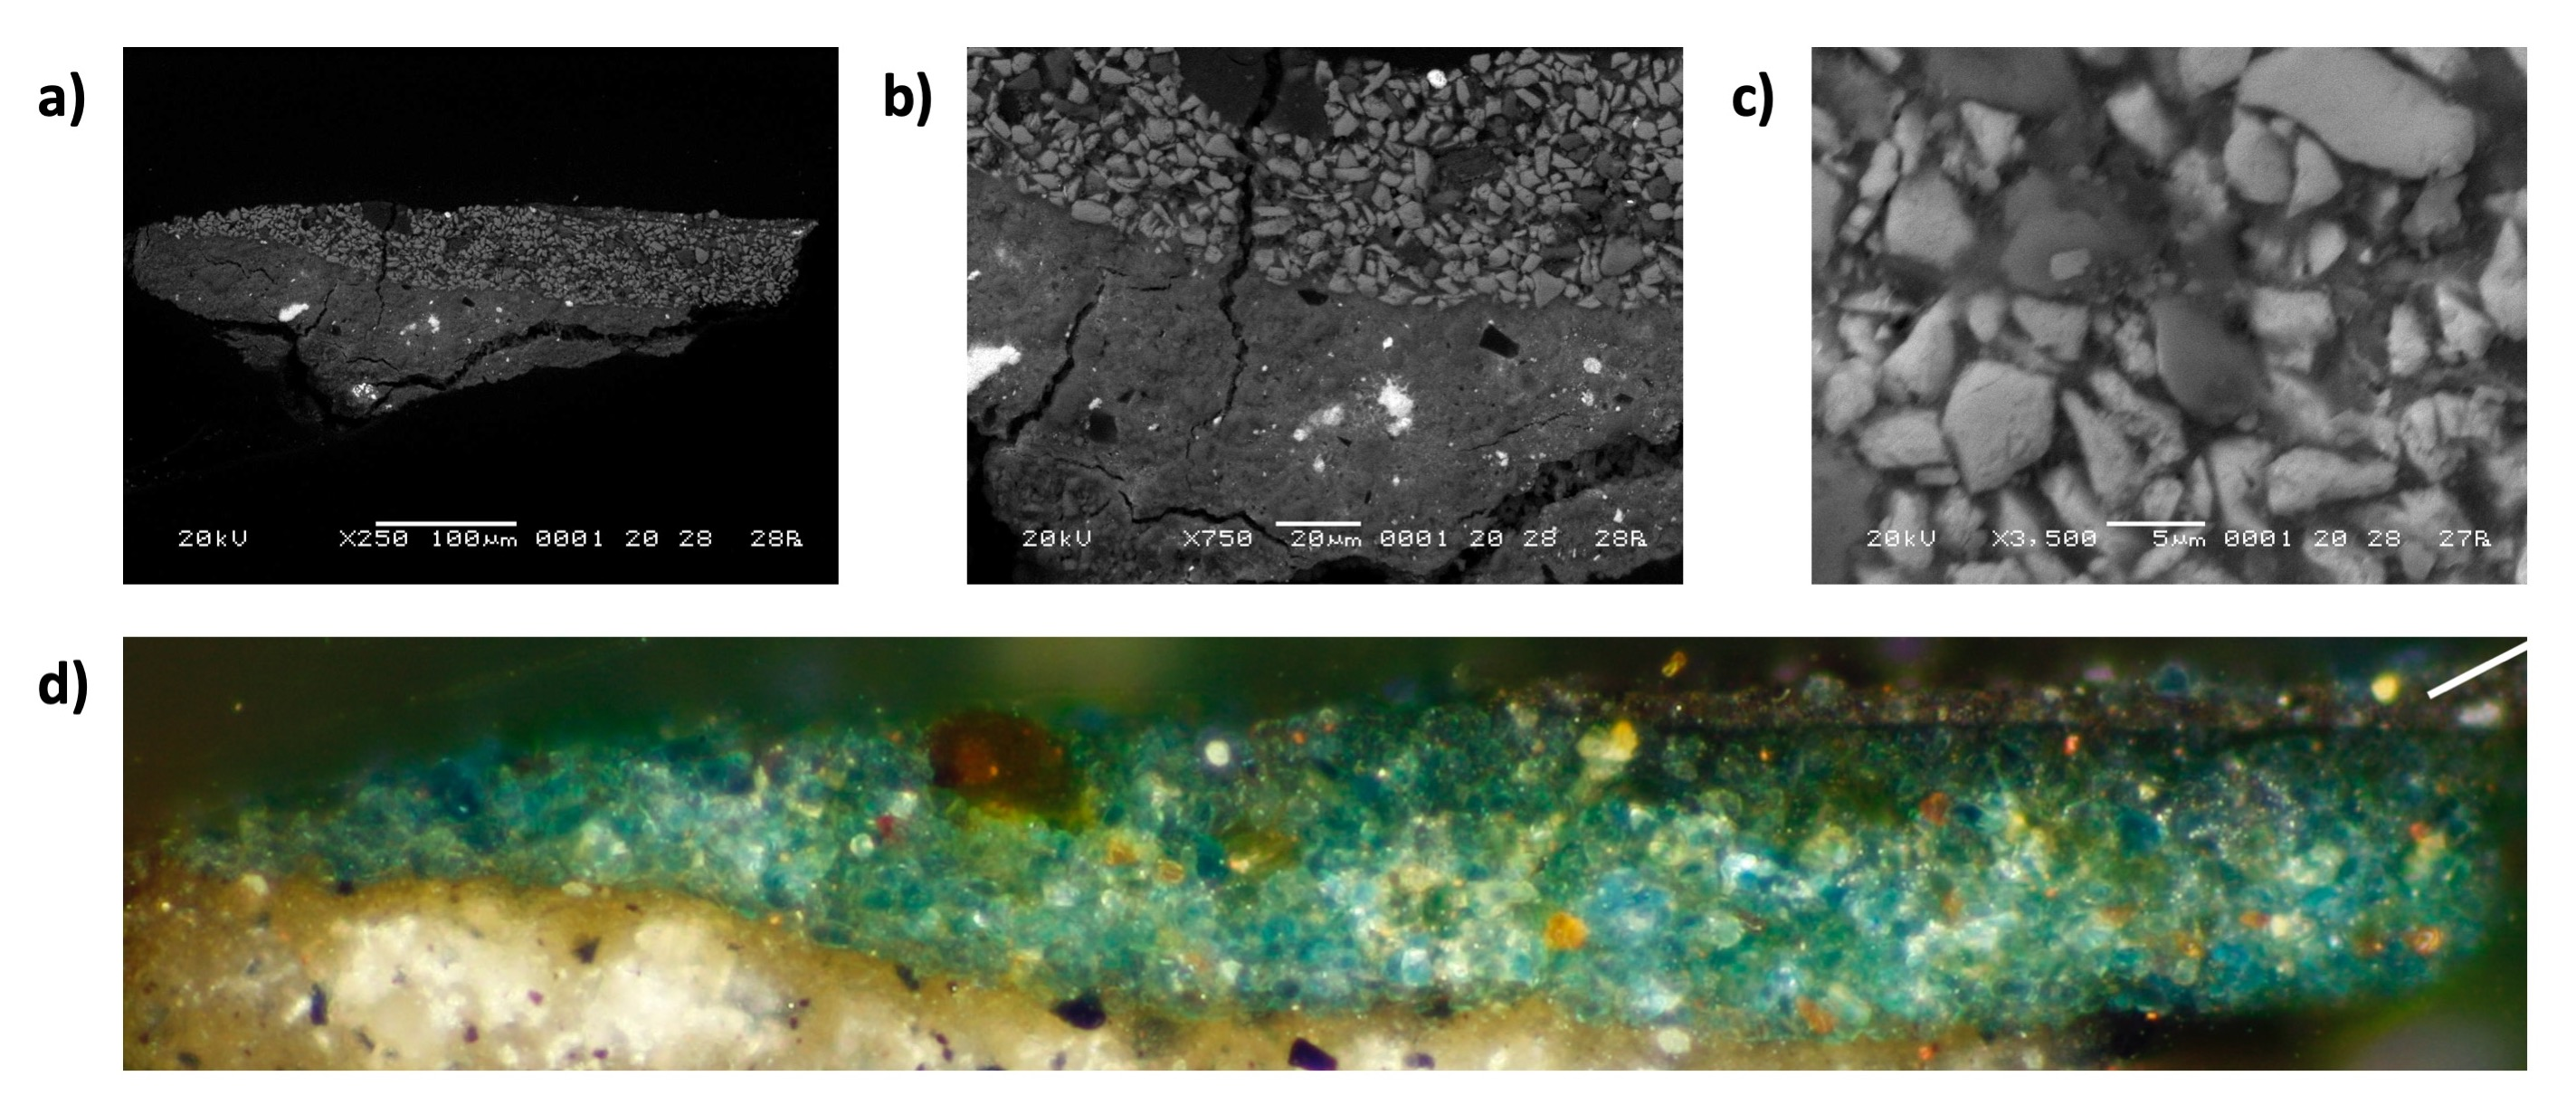
\includegraphics[width=0.8\linewidth]{1259.1_imgs}
\caption[SEM and dark-field microscope images of sample 1259.1.]{SEM and dark-field microscope images of sample 1259.1: \textbf{a)} 250x magnification, \textbf{b)} 750x magnification, \textbf{c)} 3500x magnification, \textbf{d)} dark field microscope image provided courtesy of Katharine Waldron, HKI. Distinct copper-based pigments (blue) comprise one layer, and beneath is a thick layer of white paint. A thin layer above the blue pigment is modern overpaint.}
\label{fig:1259.1_imgs}
\end{figure}

\begin{figure}[H]
\centering
\begin{minipage}[t]{\linewidth}
  \centering
  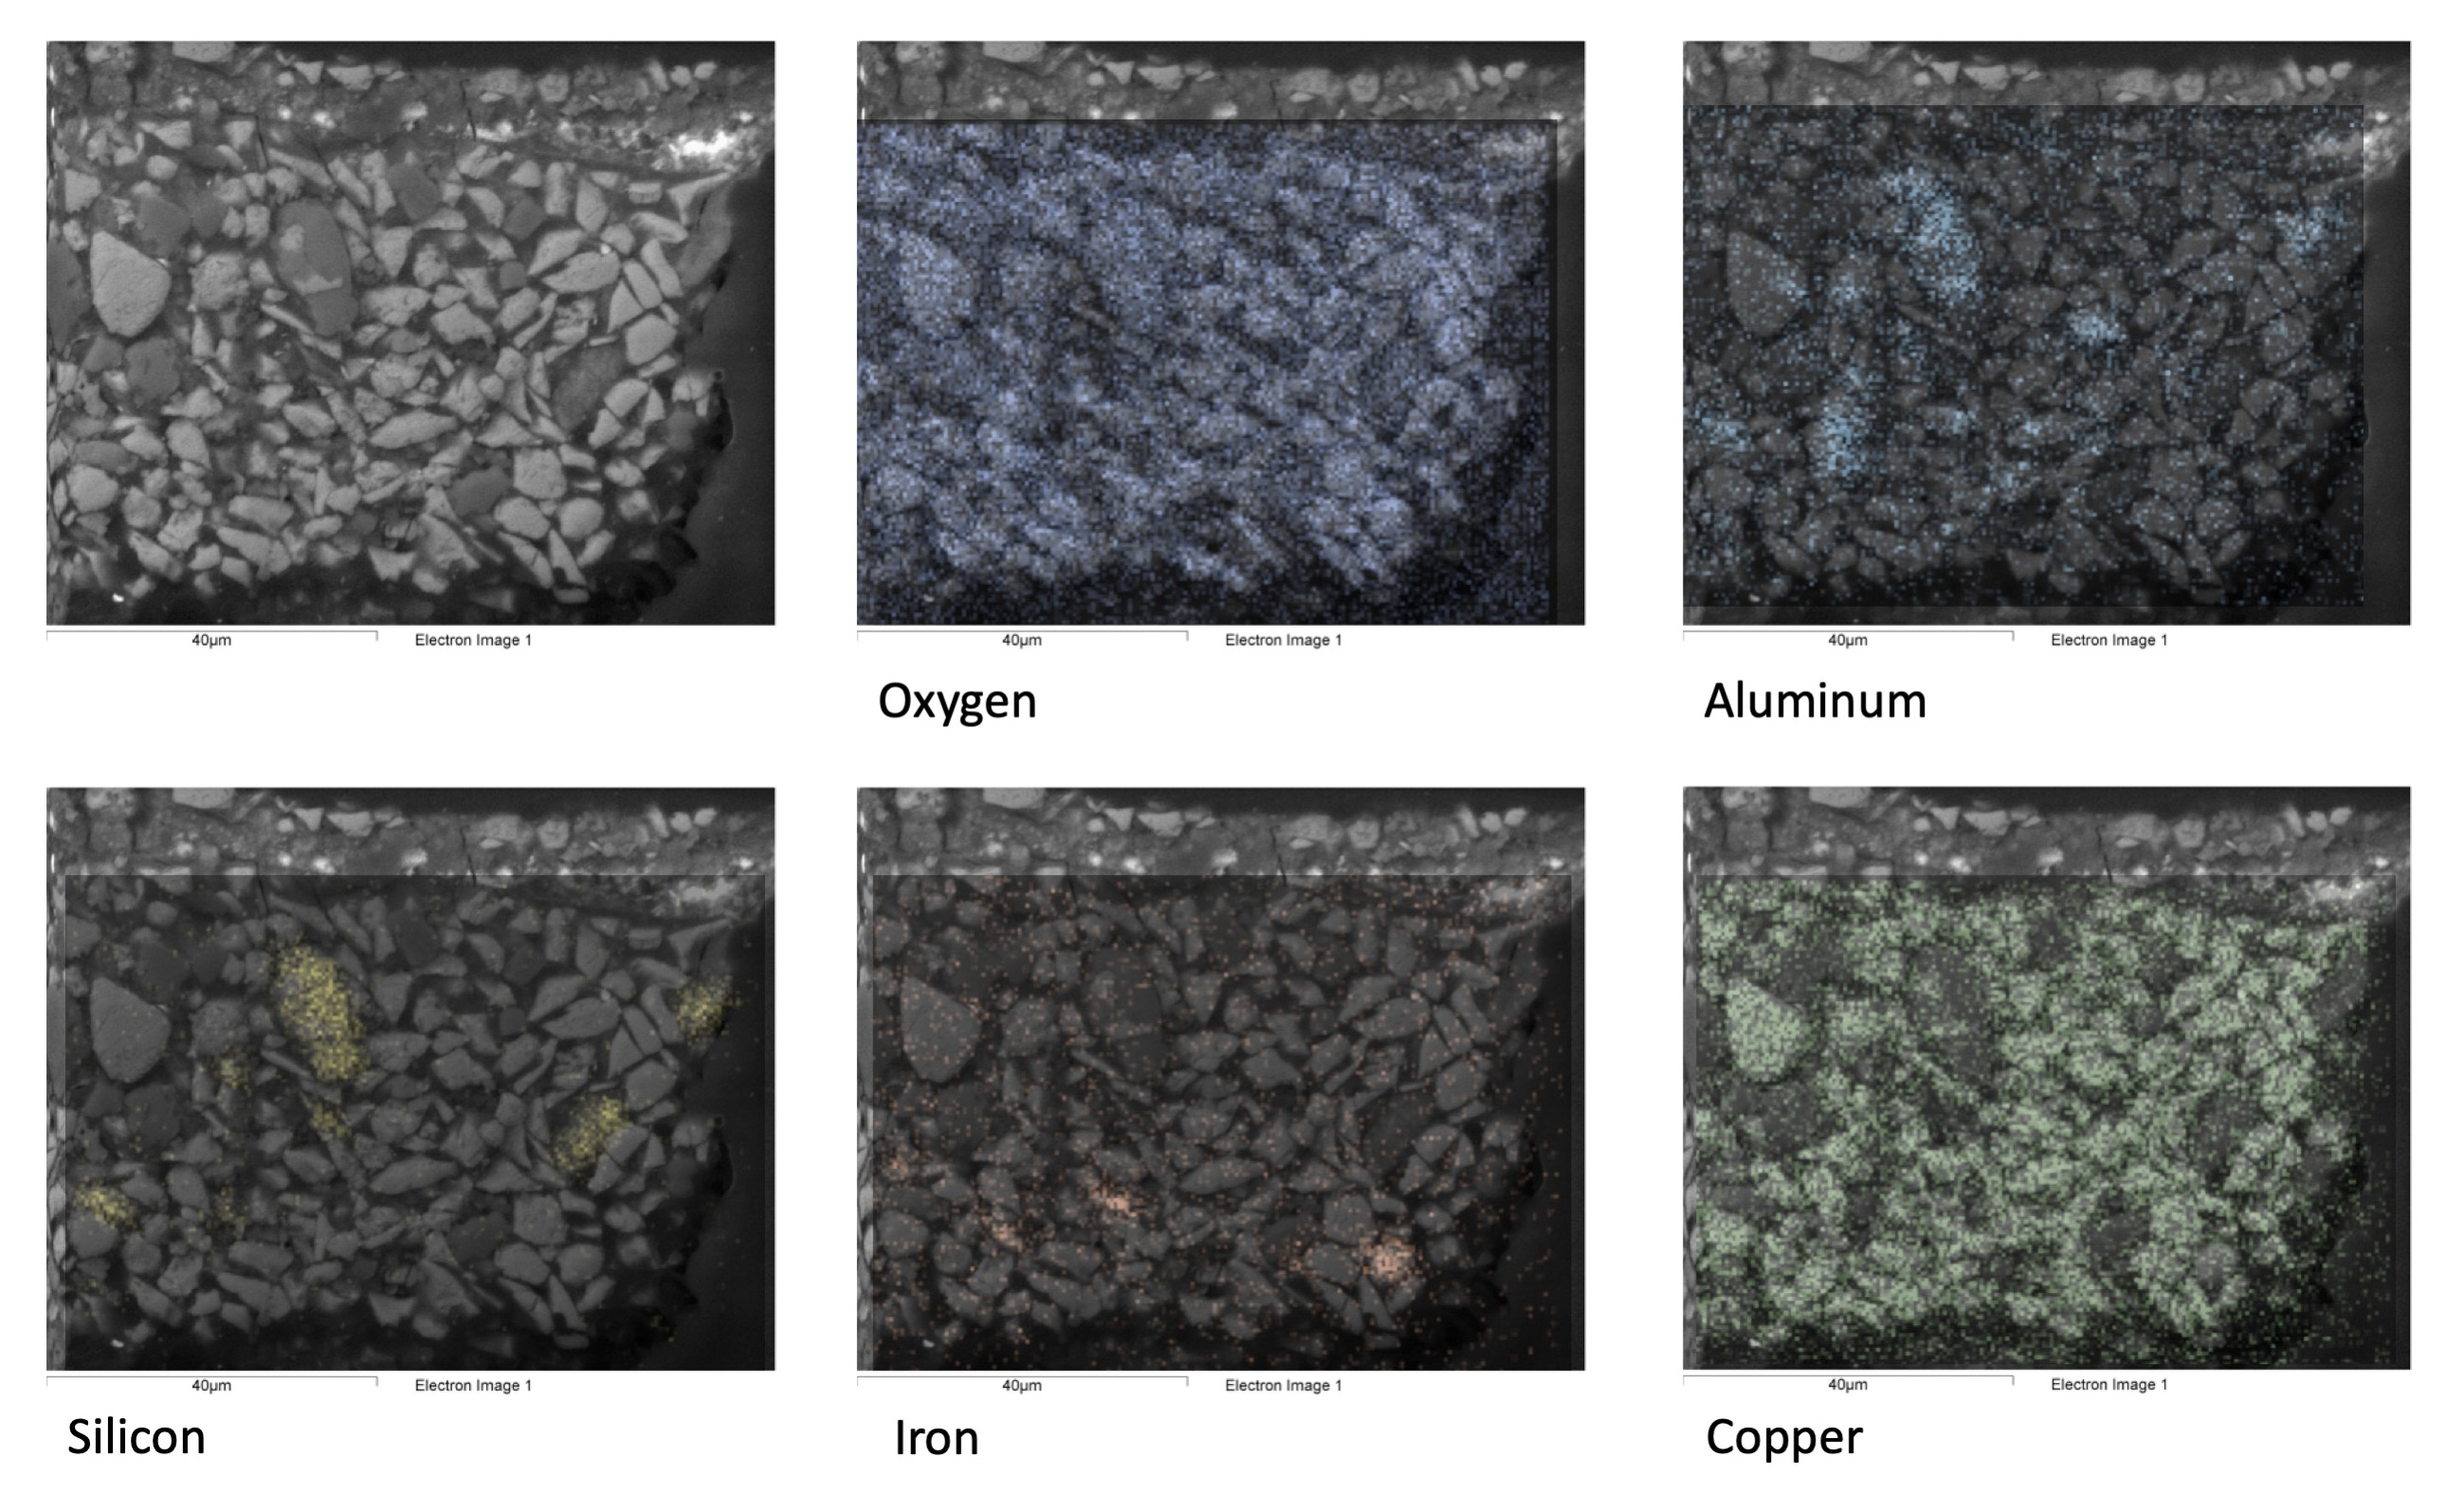
\includegraphics[width=0.9\linewidth]{1259.1_mapdata_1}
\hfill
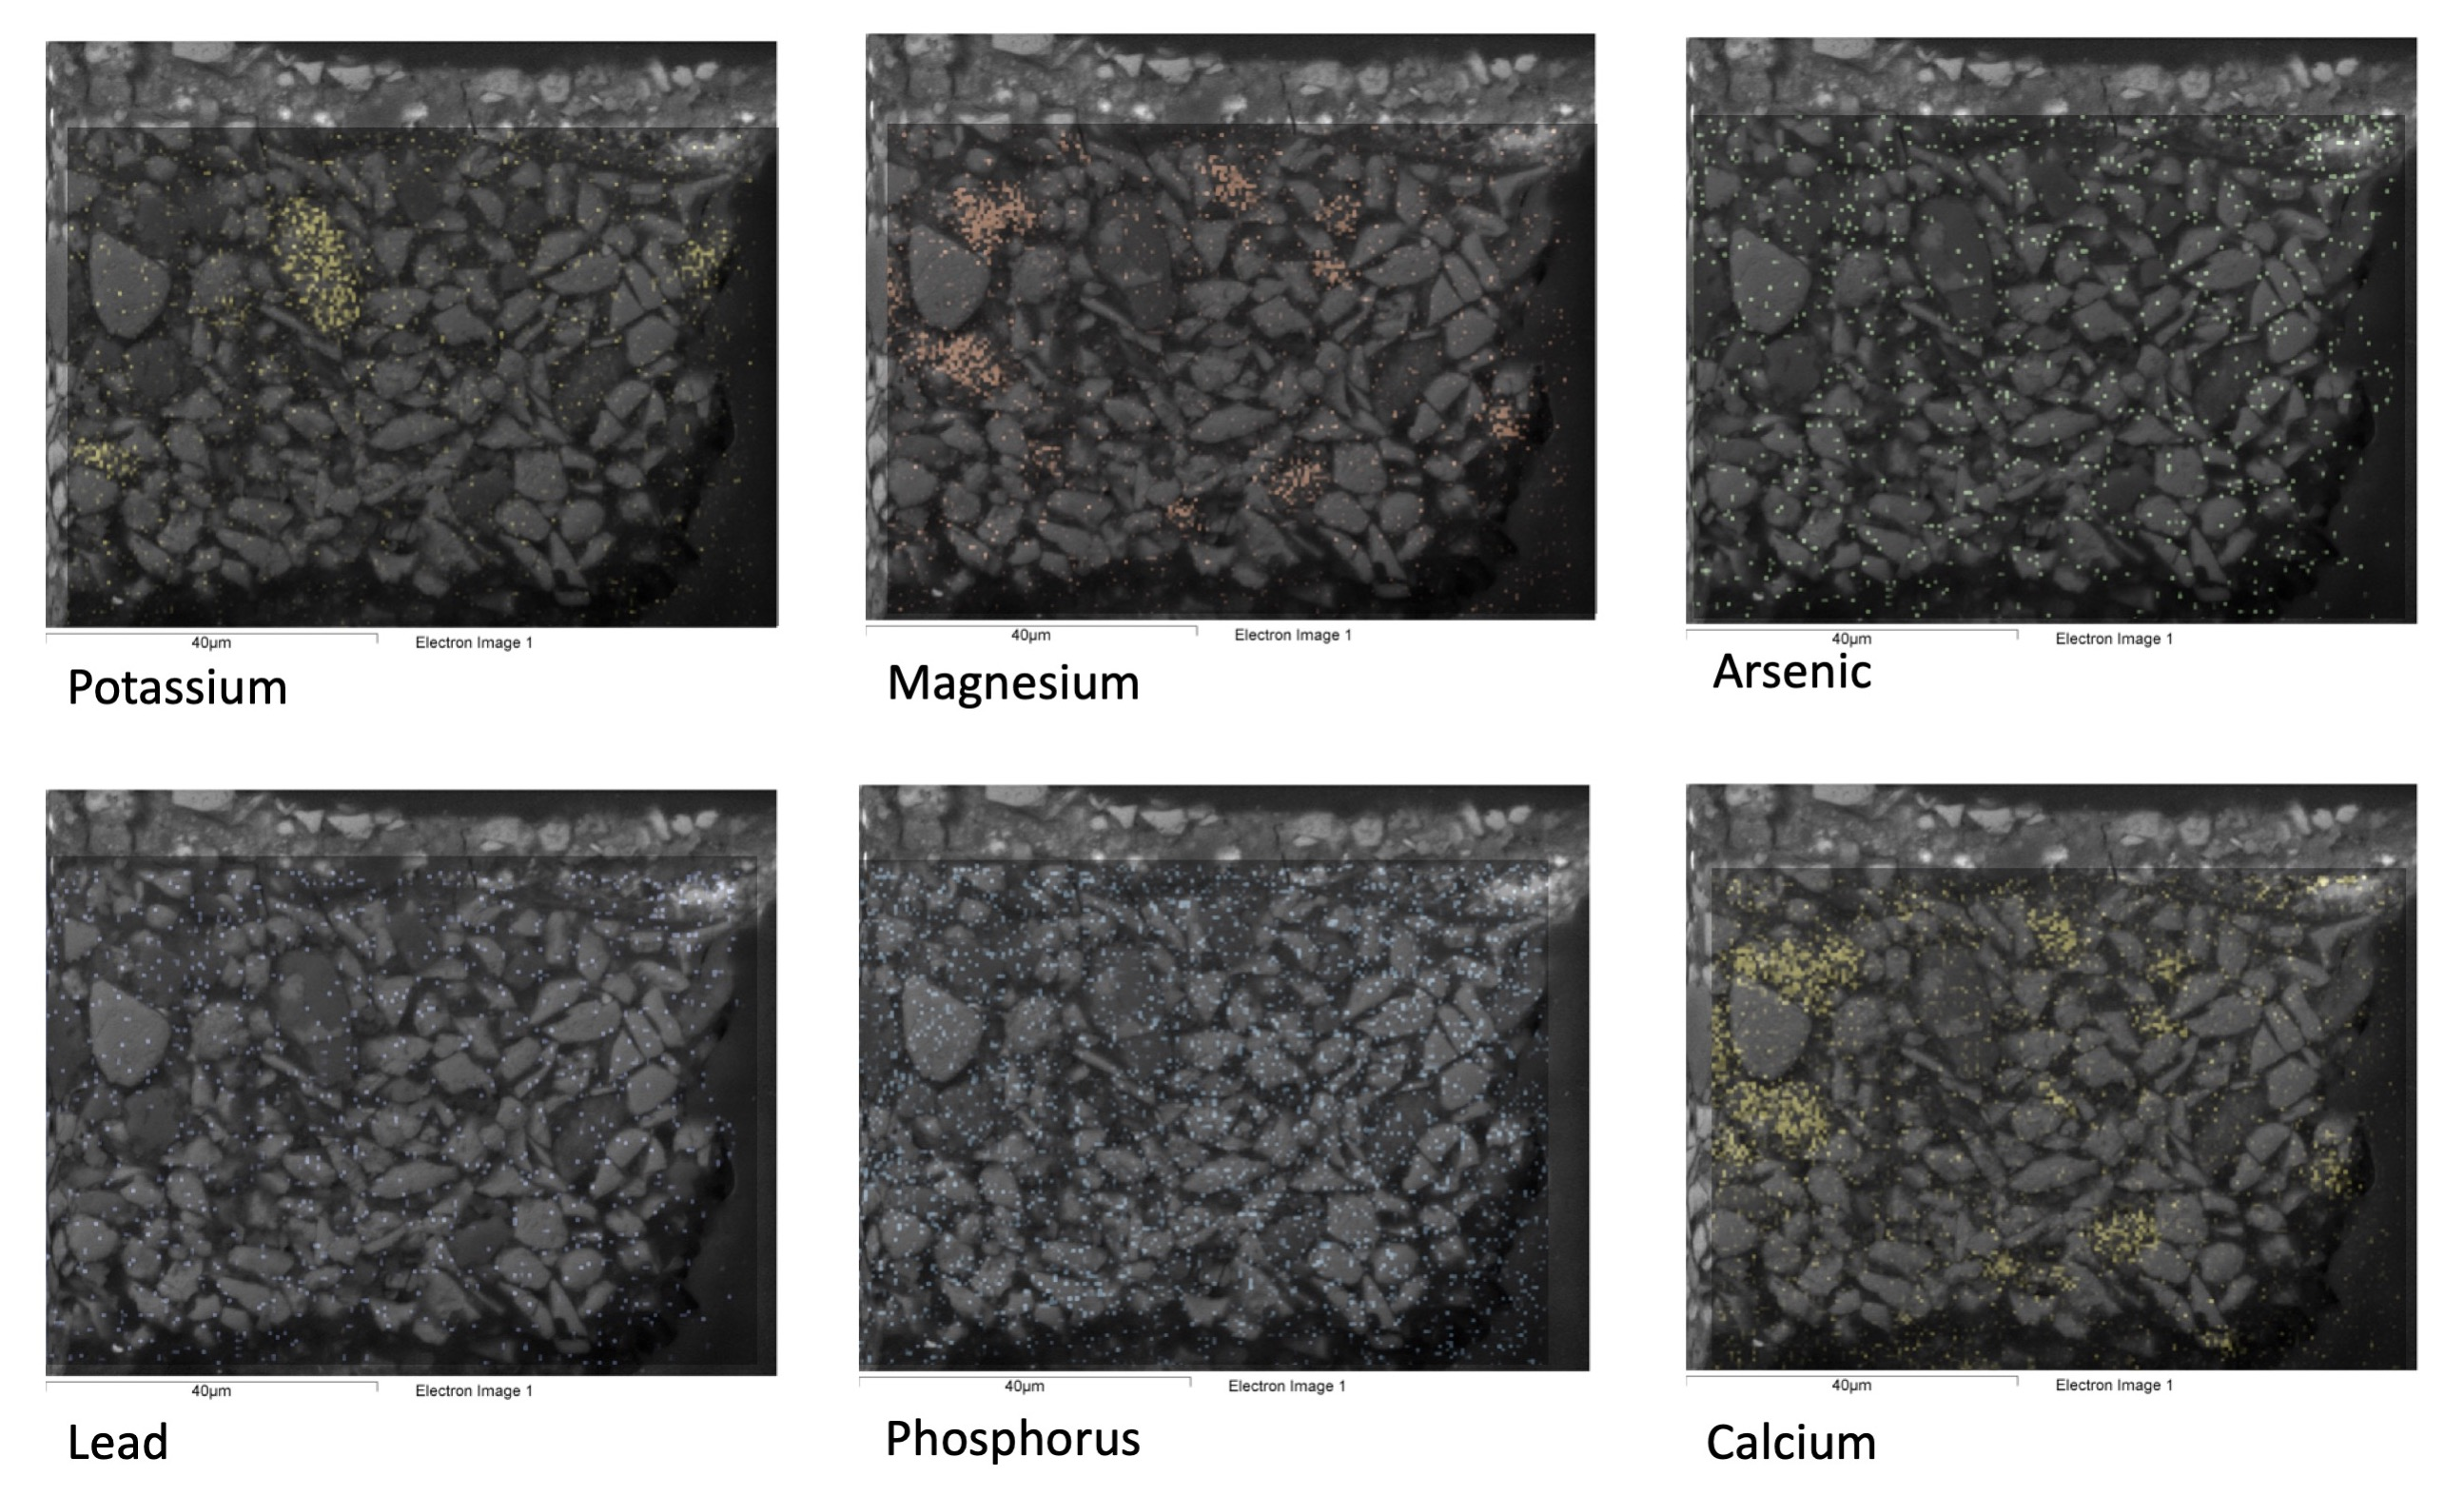
\includegraphics[width=0.9\linewidth]{1259.1_mapdata_2}
\hfill
\end{minipage}
\caption[EDS map data, sample 1259.1.]{EDS map data of sample 1259.1 showing locations of elements in an area of the azurite paint layer. Elements detected are O, Al, Si, Fe, Cu, K, Mg, As, Pb, P, and Ca.}
\label{fig:1259.1_mapdata}
\end{figure}

\begin{figure}[H]
\centering
  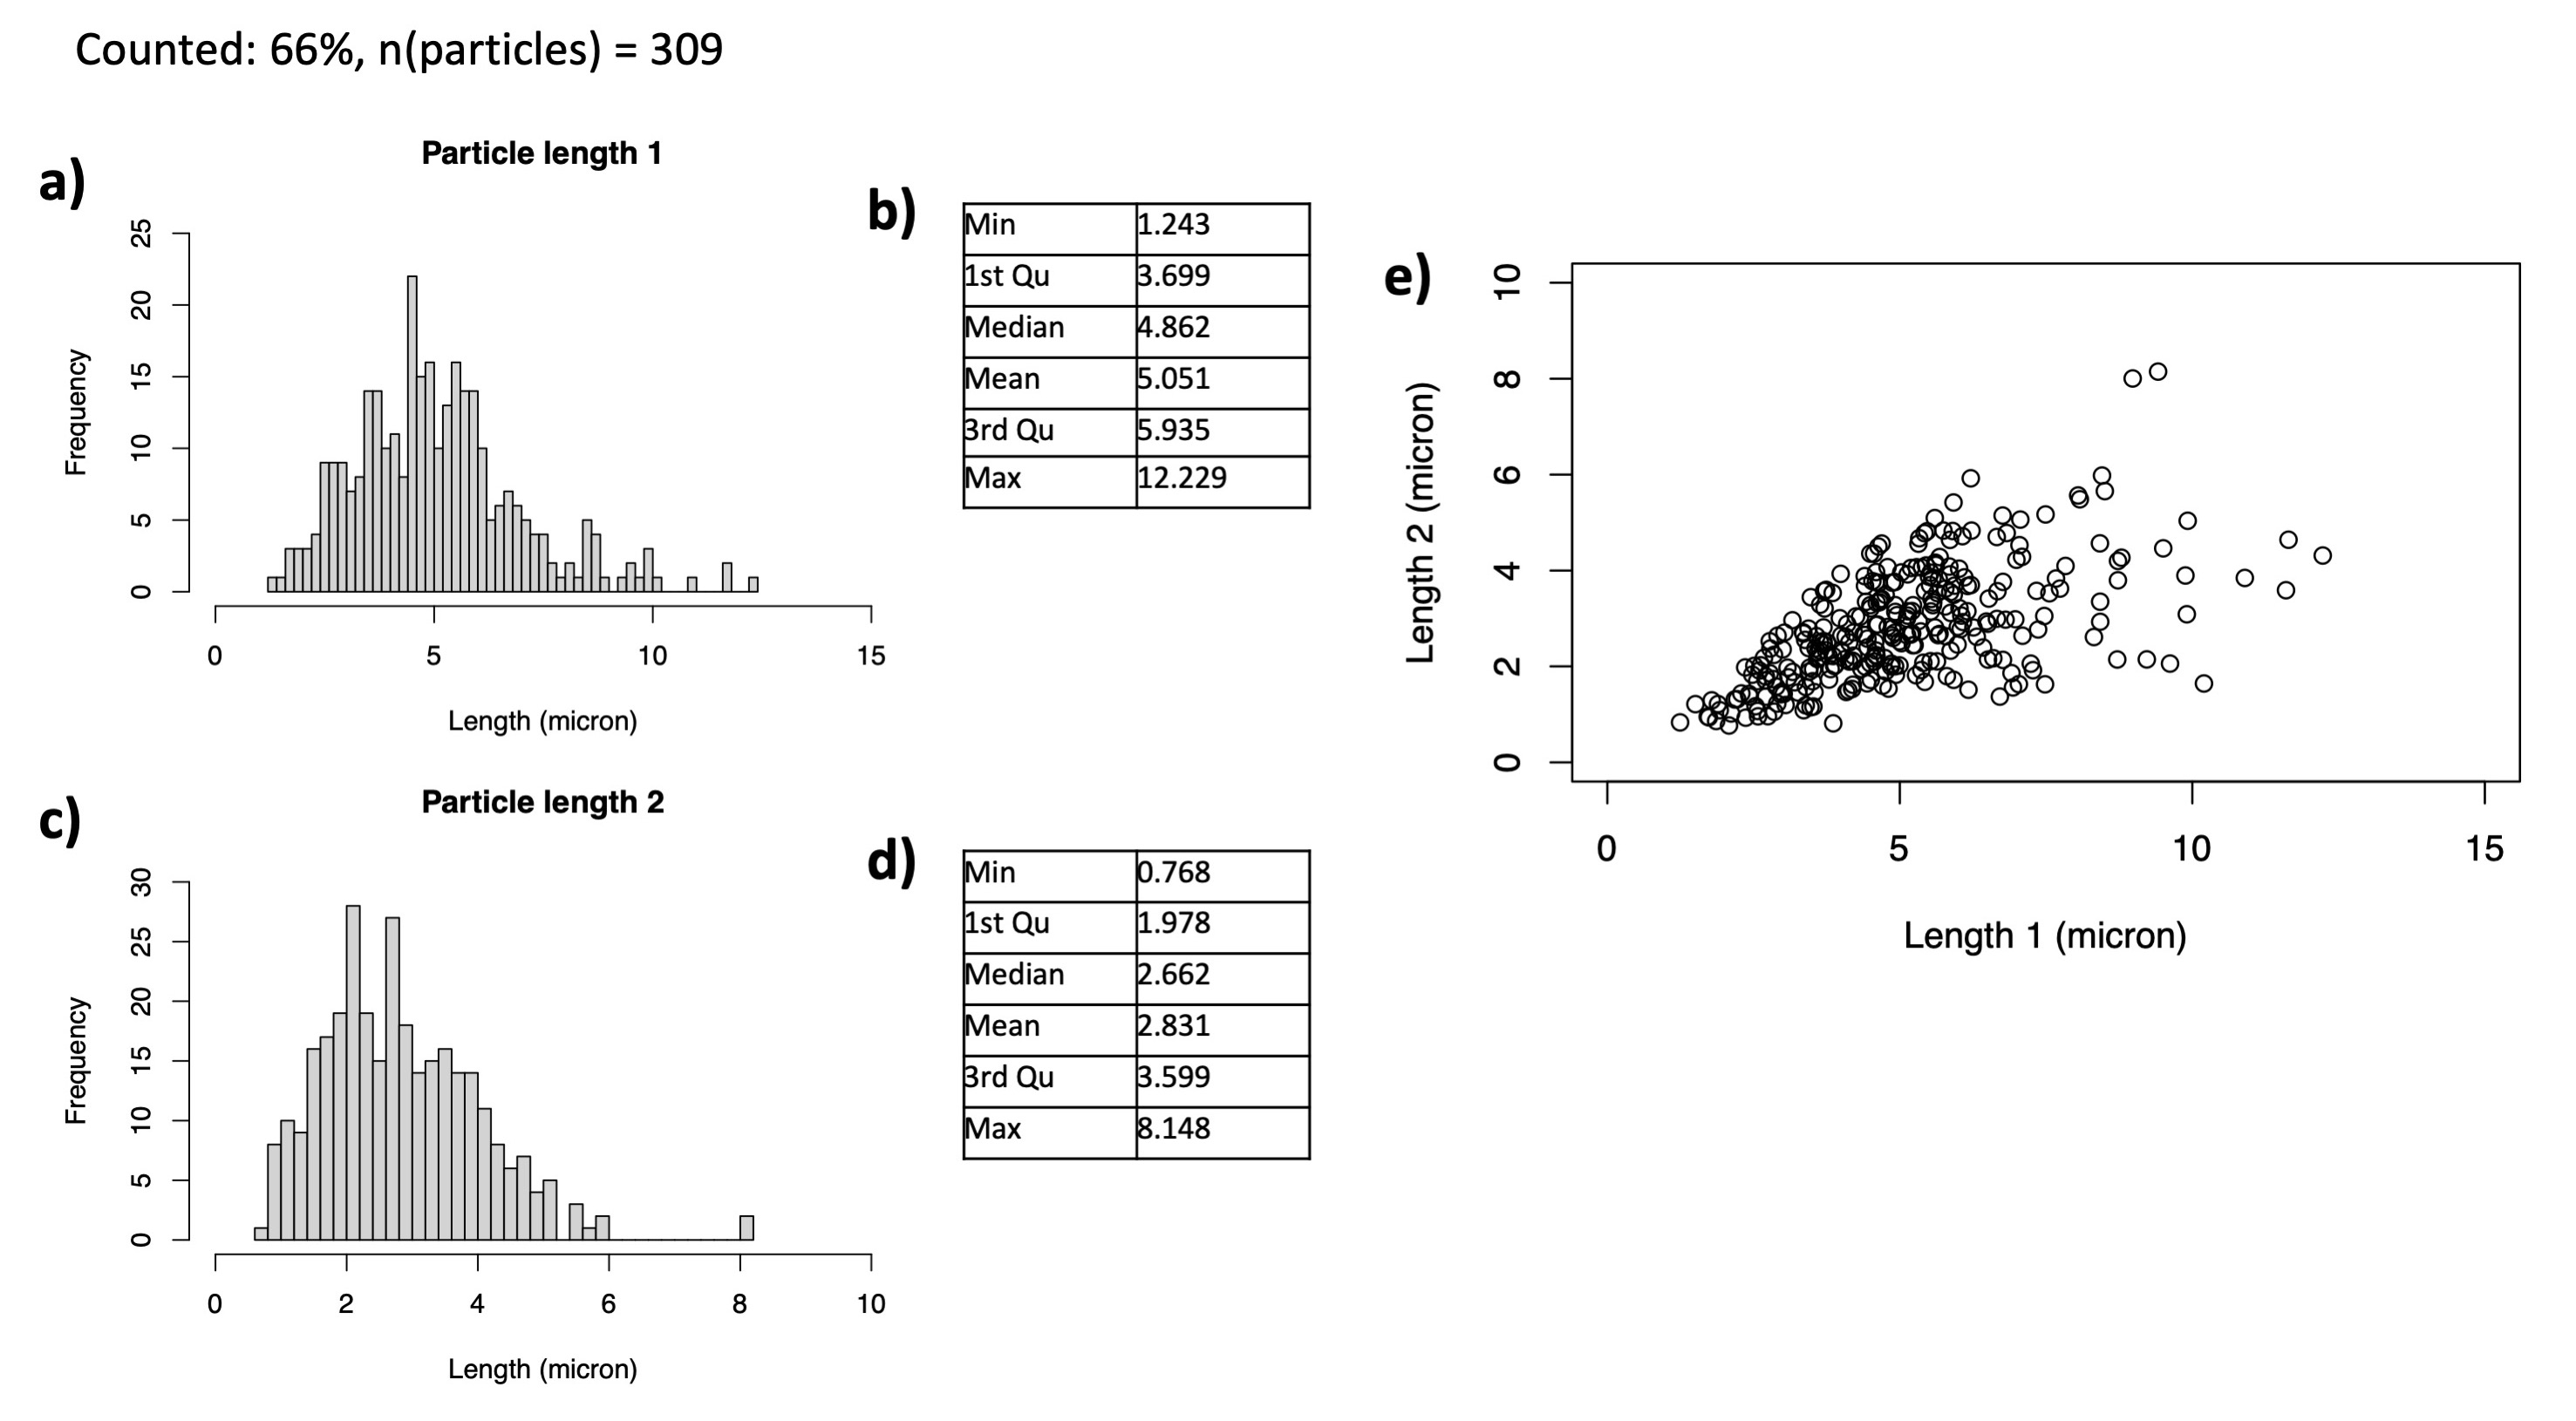
\includegraphics[width=0.8\linewidth]{1259.1_partsize}
\caption[Particle size distribution, sample 1259.1.]{Particle size distribution of sample 1259.1: \textbf{a)} Histogram showing distribution of particle length 1 values, taken as the longest dimension. \textbf{b)} Descriptive statistics for particle length 1 data. \textbf{c)} Histogram showing distribution of particle length 2 values, taken as the longest distance perpendicular to length 1. \textbf{d)} Descriptive statistics for particle length 2 data. \textbf{e)} Graph of length 1 versus length 2 showing the degree of skew of azurite particles.}
\label{fig:1259.1_partsize}
\end{figure}




\section{Sample 1259.6}

\begin{figure}[H]
  \centering
  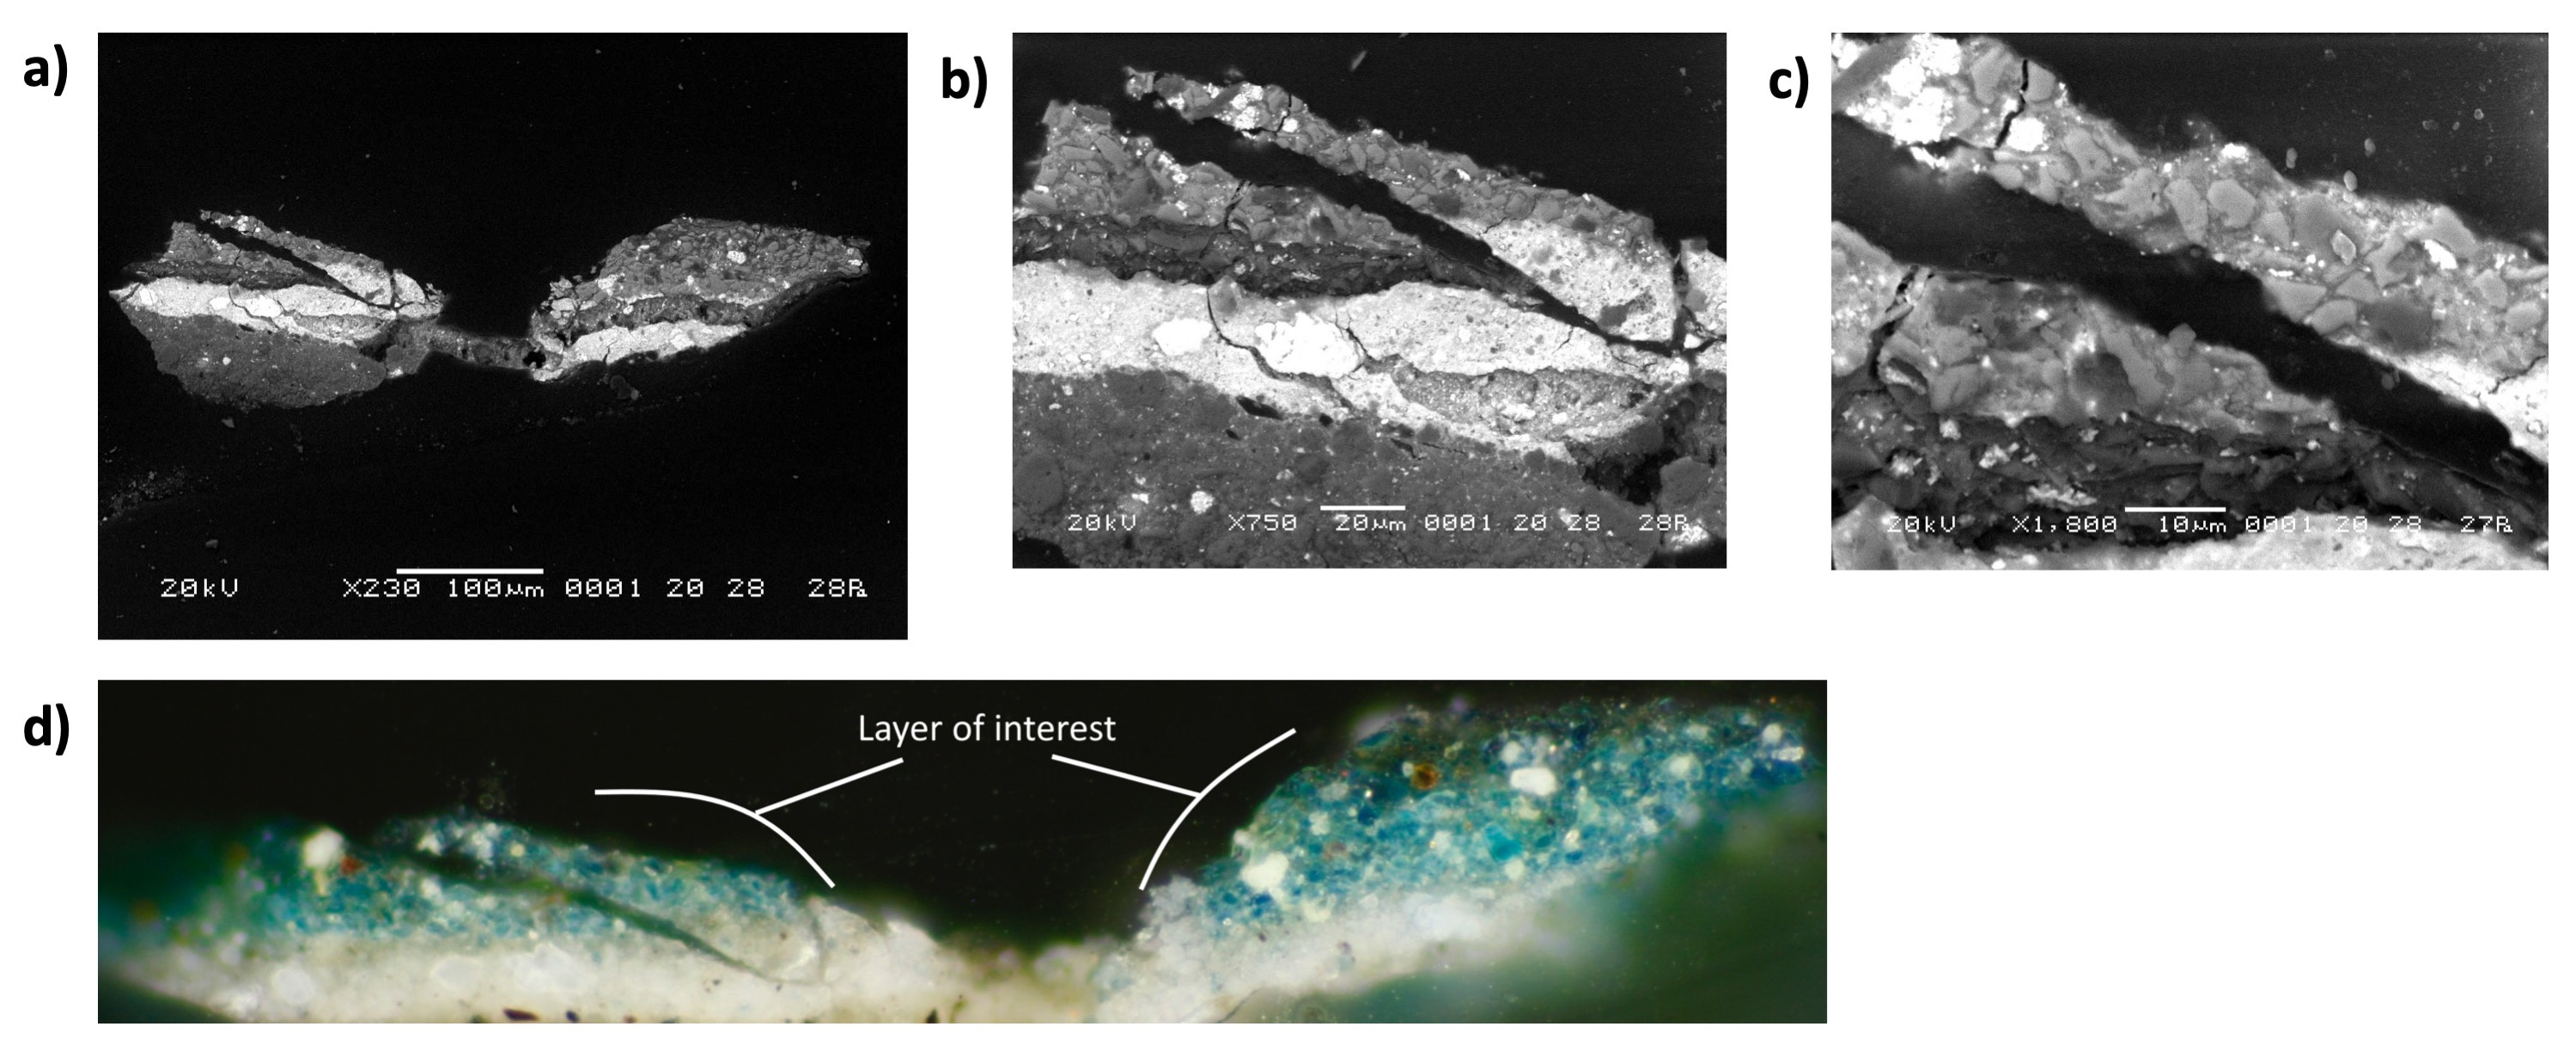
\includegraphics[width=0.8\linewidth]{1259.6_imgs}
\caption[SEM and dark-field microscope images of sample 1259.6.]{SEM and dark-field microscope images of sample 1259.6: \textbf{a)} 230x magnification, \textbf{b)} 750x magnification, \textbf{c)} 1800x magnification, \textbf{d)} dark field microscope image provided courtesy of Katharine Waldron, HKI. A thick blue layer of azurite pigment is observed over a white base layer. The middle of the blue layer is missing.}
\label{fig:1259.6_imgs}
\end{figure}


\begin{figure}[H]
\centering
  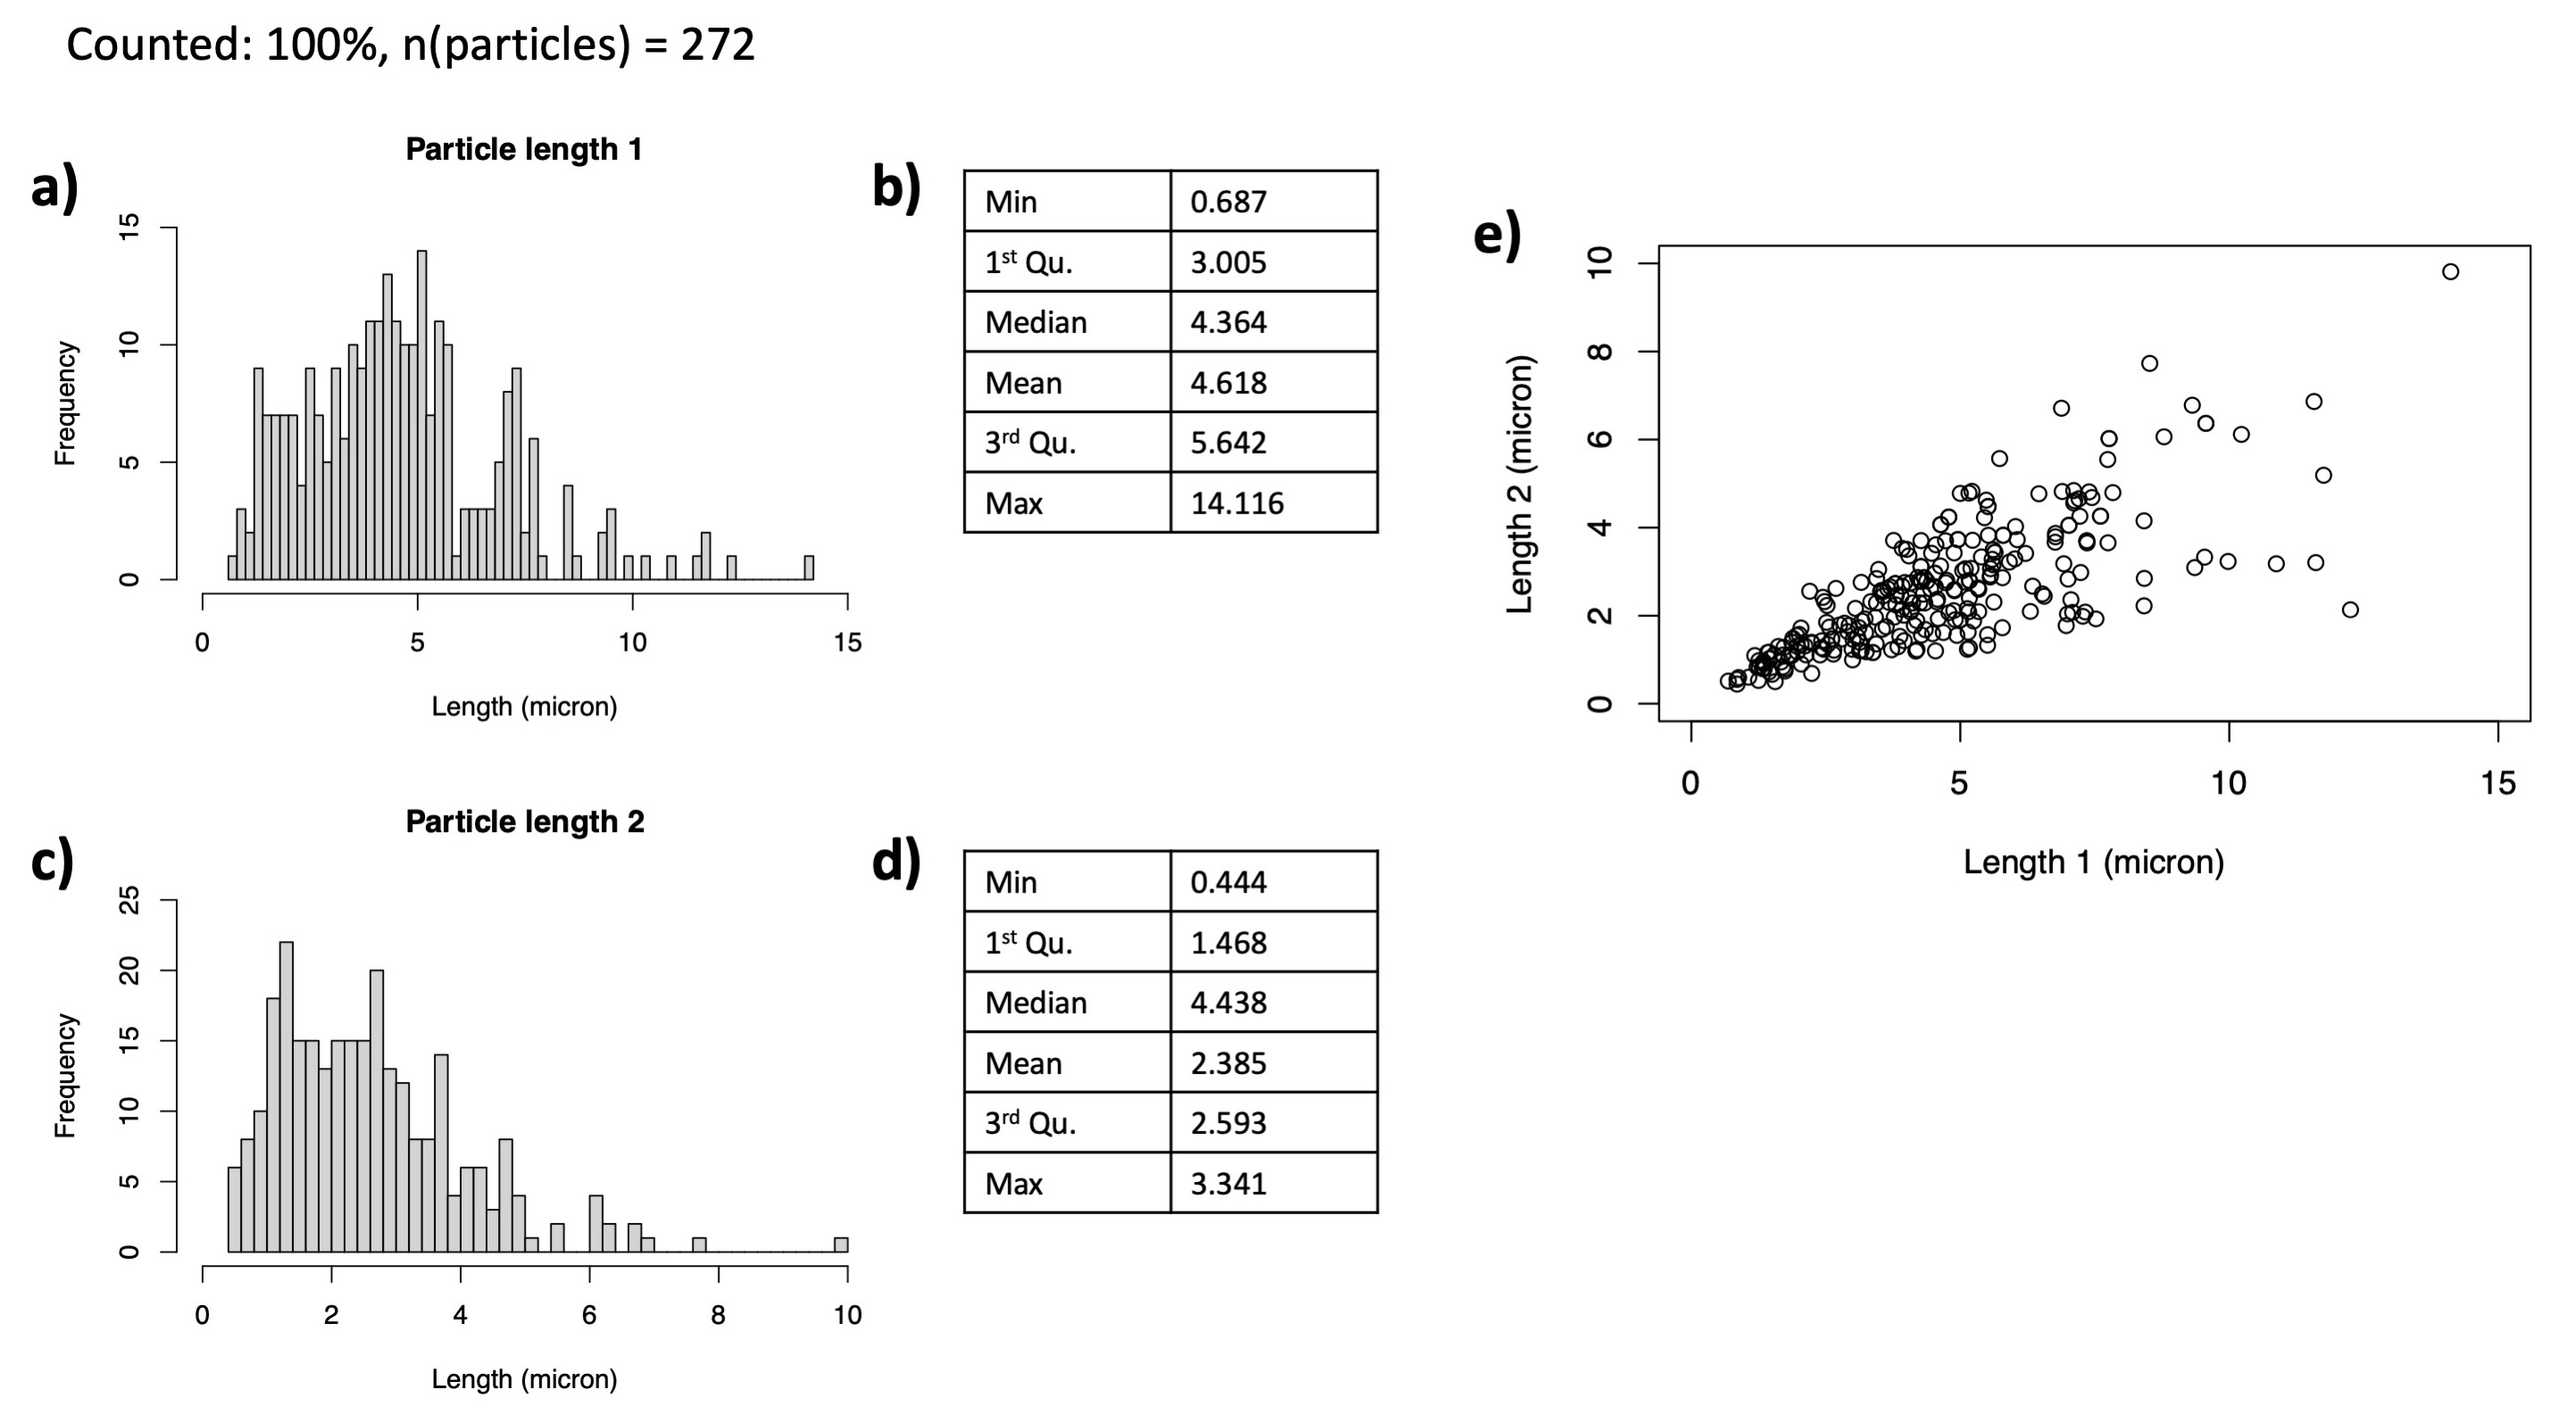
\includegraphics[width=0.8\linewidth]{1259.6_partsize}
\caption[Particle size distribution, sample 1259.6.]{Particle size distribution of sample 1259.6: \textbf{a)} Histogram showing distribution of particle length 1 values. \textbf{b)} Descriptive statistics for particle length 1 data. \textbf{c)} Histogram showing distribution of particle length 2 values. \textbf{d)} Descriptive statistics for particle length 2 data. \textbf{e)} Graph of length 1 versus length 2 showing the degree of skew.}
\label{fig:1259.6_partsize}
\end{figure}




\section{Sample 1259.14}

\begin{figure}[H]
  \centering
  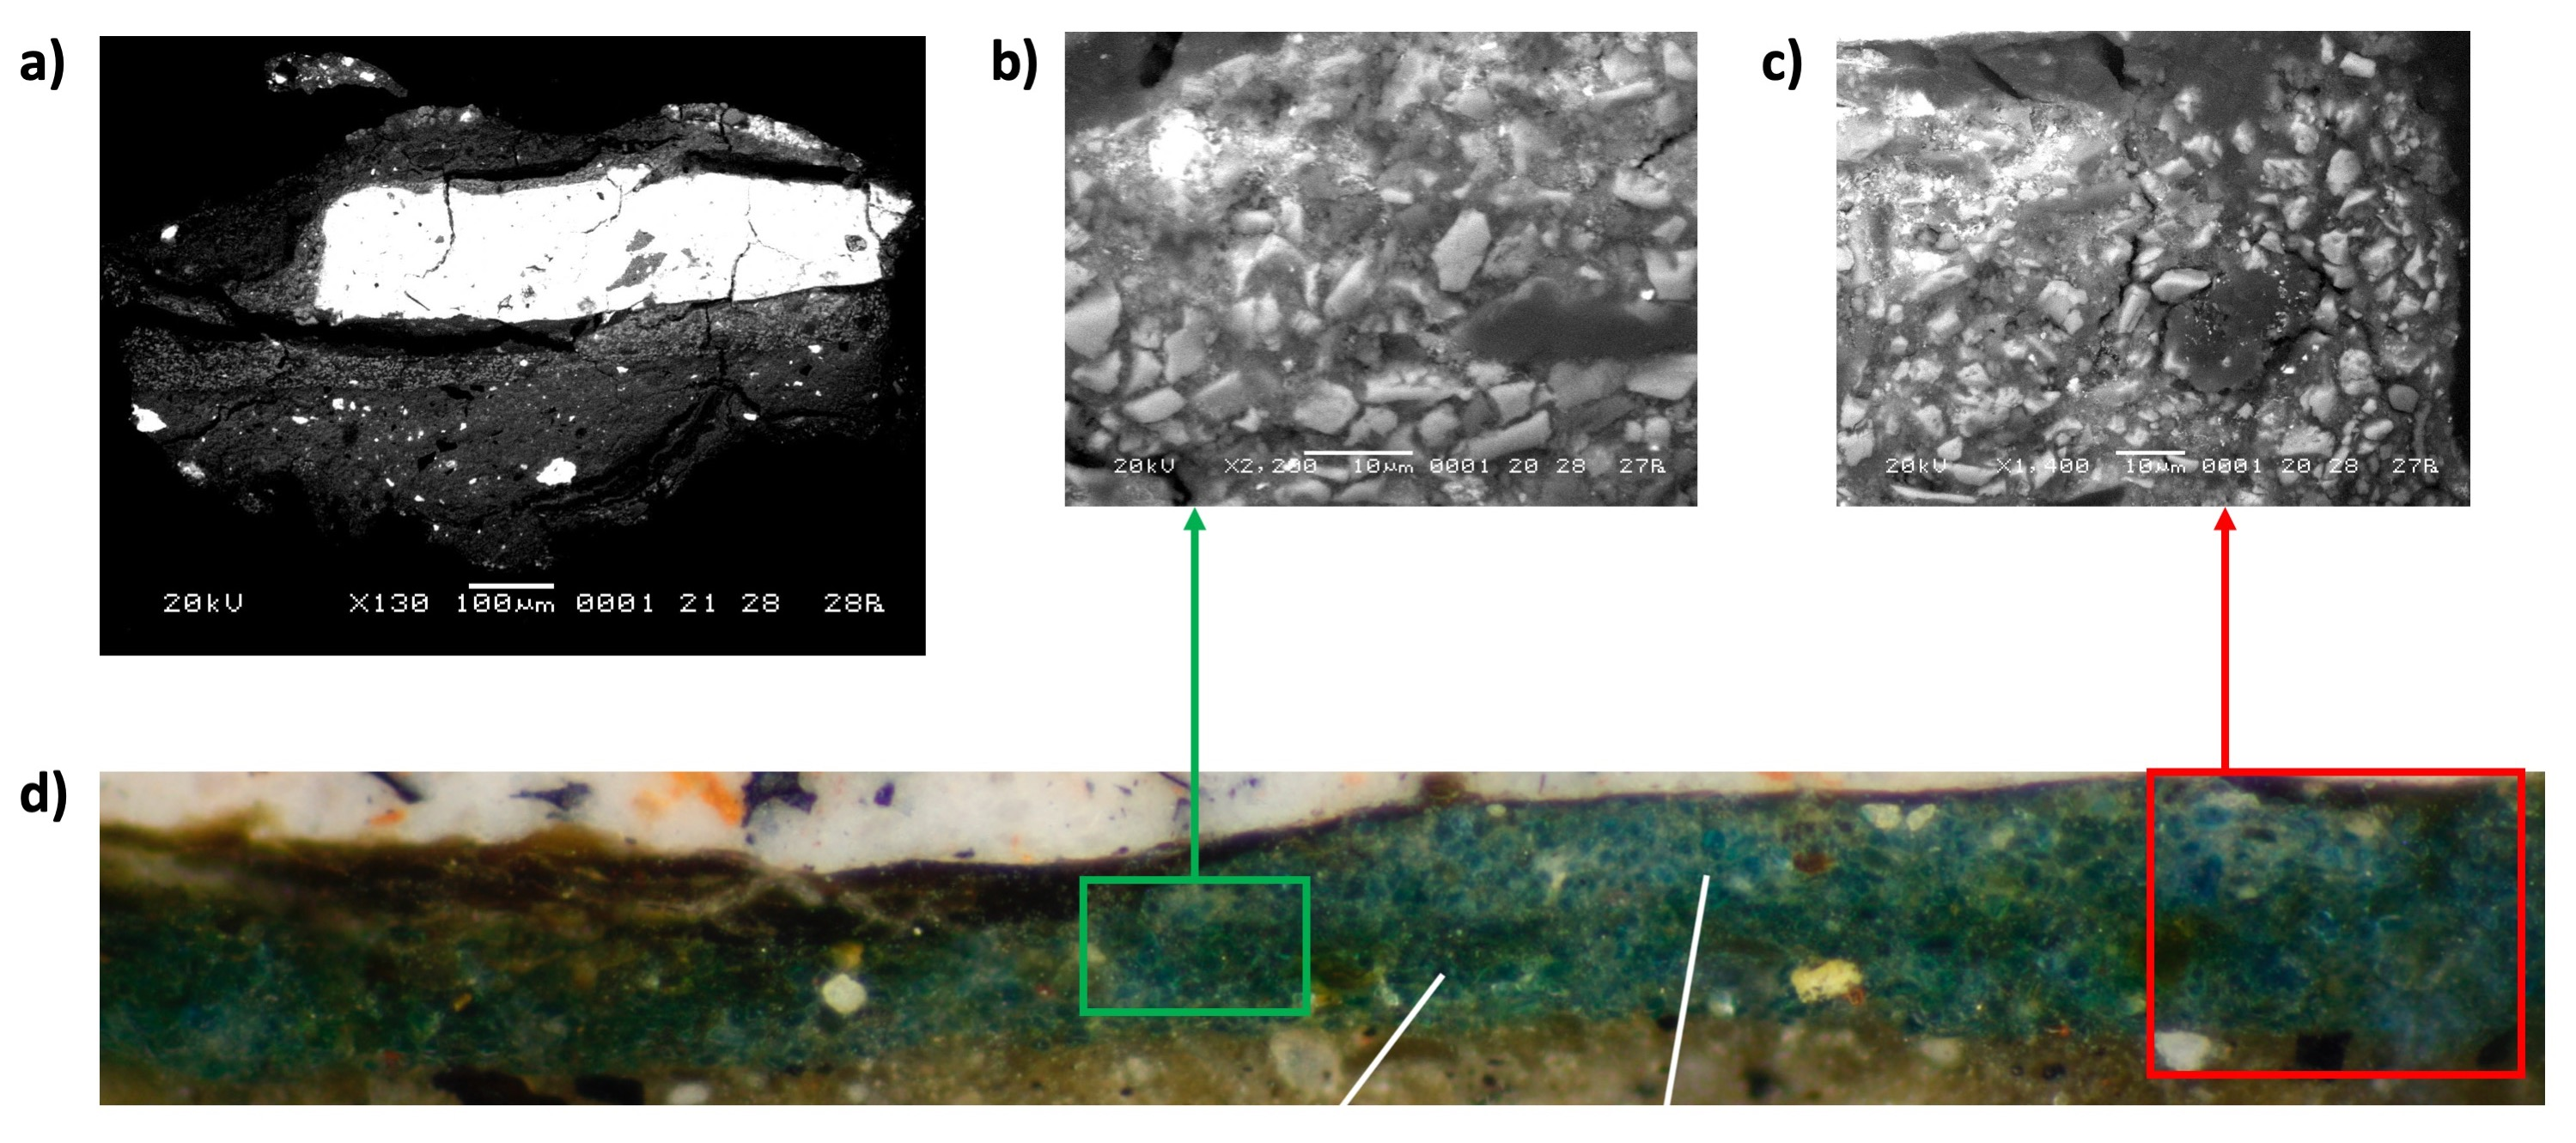
\includegraphics[width=0.8\linewidth]{1259.14_imgs}
\caption[SEM and dark-field microscope images of sample 1259.14.]{SEM and dark-field microscope images of sample 1259.14: \textbf{a)} 130x magnification, \textbf{b)} 2200x magnification, \textbf{c)} 1400x magnification, \textbf{d)} dark field microscope image provided courtesy of Katharine Waldron, HKI. The SEM images in \textbf{b)} and \textbf{c)} show areas on the dark field image that are demarcated by green and red boxes. Two distinct layers of azurite particles are shown, the lower one extending the length of the cross section.}
\label{fig:1259.14_imgs}
\end{figure}

\begin{figure}[H]
\centering
\begin{minipage}[t]{\linewidth}
  \centering
  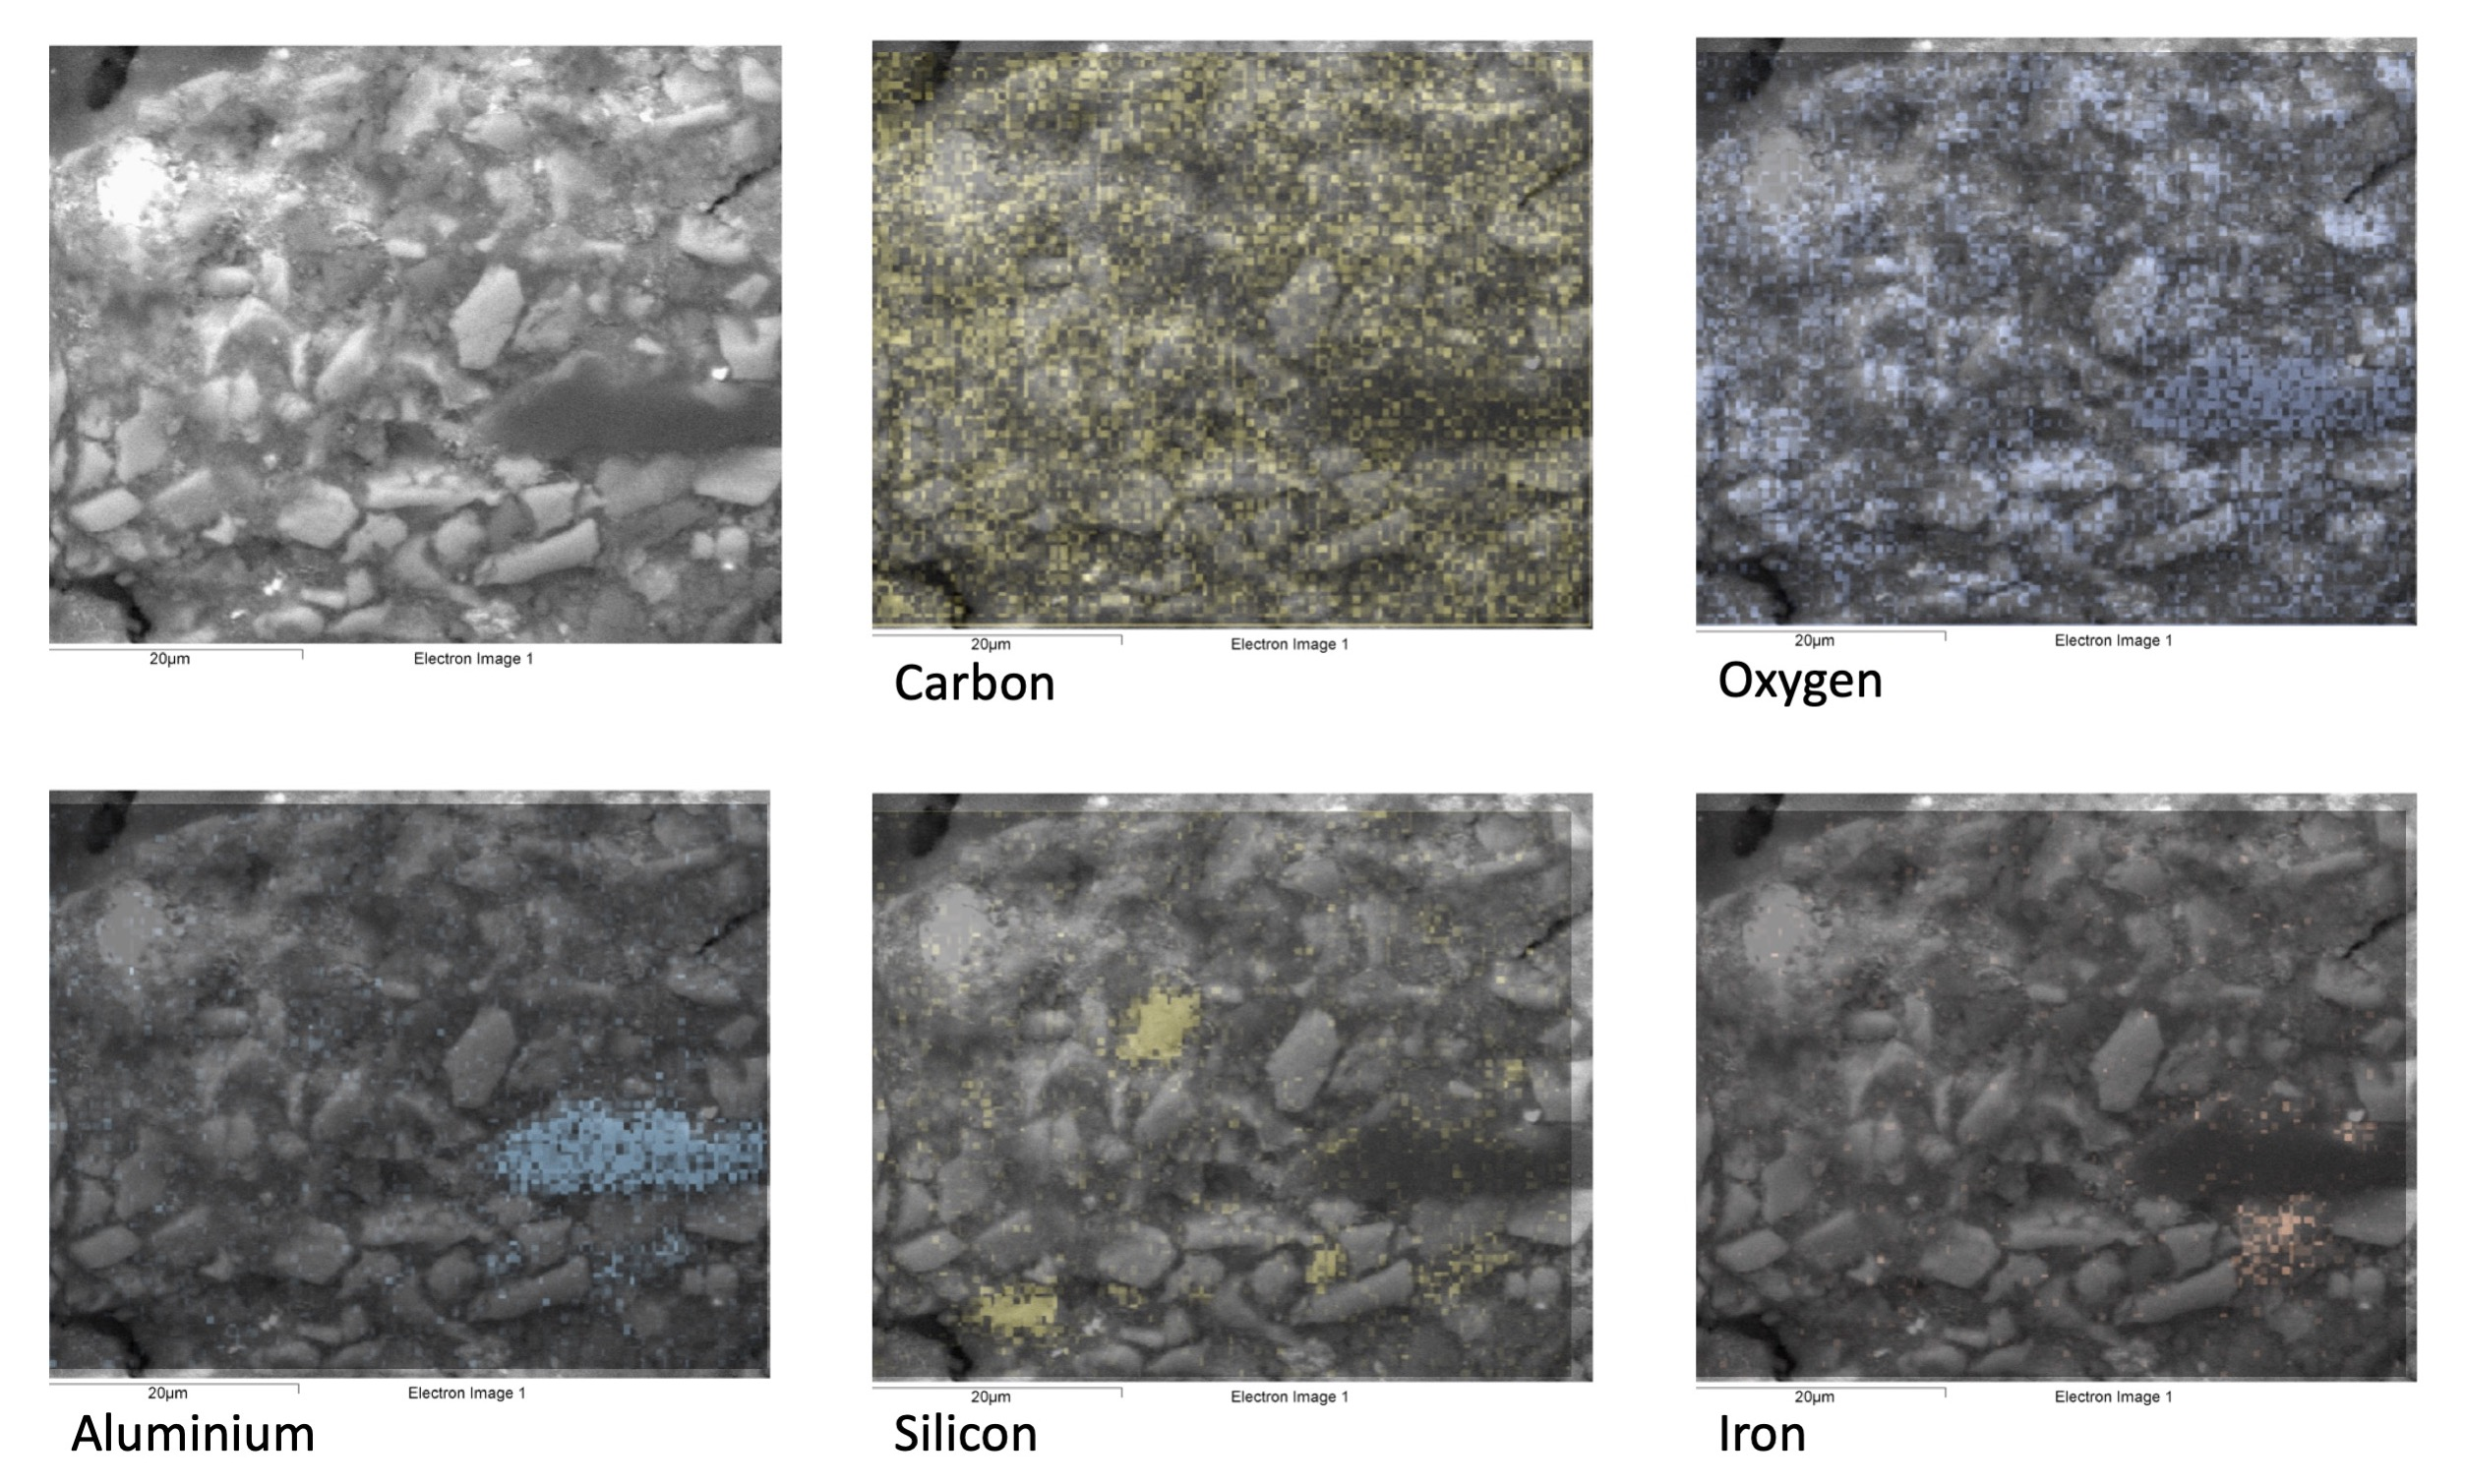
\includegraphics[width=0.9\linewidth]{1259.14_mapdata_1}
\hfill
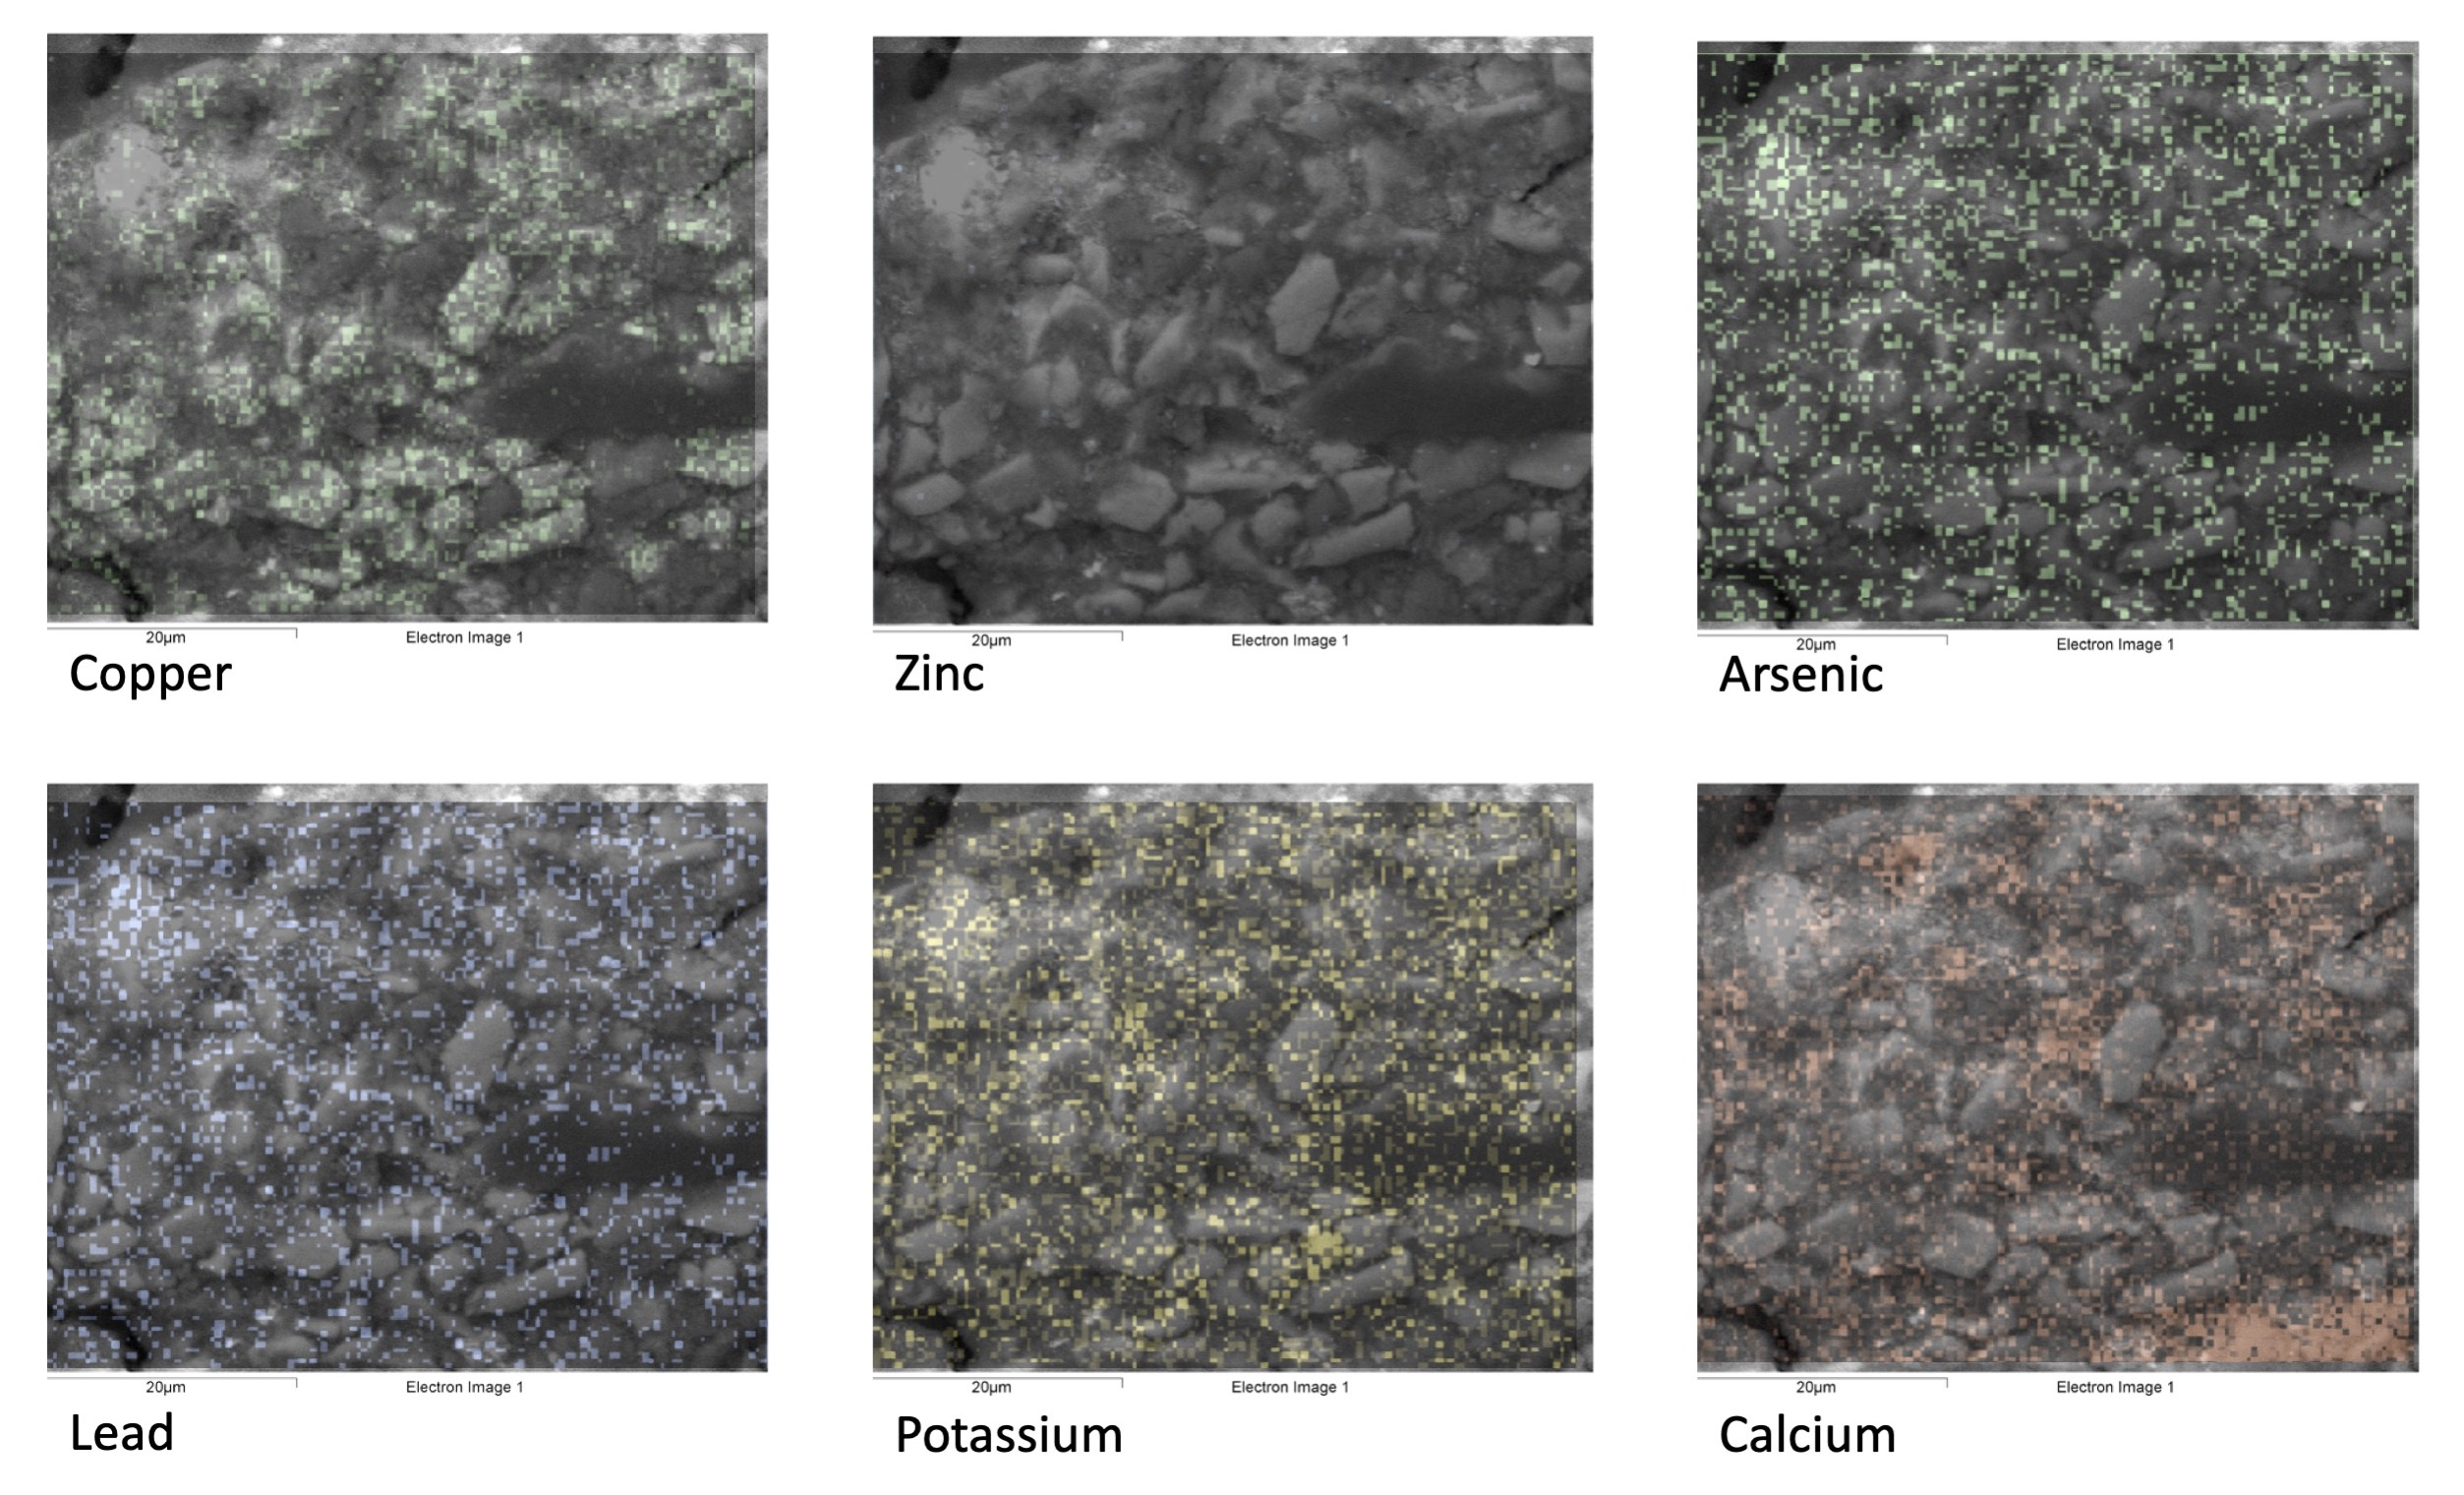
\includegraphics[width=0.9\linewidth]{1259.14_mapdata_2}
\hfill
\end{minipage}
\caption[EDS map data, sample 1259.14.]{EDS map data of sample 1259.14 showing locations of elements in an area of the azurite paint layer. Elements detected are C, O, Al, Si, Fe, Cu, Zn, As, Pb, K, and Ca.}
\label{fig:1259.14_mapdata}
\end{figure}

\begin{figure}[H]
\centering
  \includegraphics[width=0.8\linewidth]{1259.1_partsize_1}
\caption[Particle size distribution, sample 1259.14 bottom layer.]{Particle size distribution of sample 1259.14, bottom layer of azurite: \textbf{a)} Histogram showing distribution of particle length 1 values. \textbf{b)} Descriptive statistics for particle length 1 data. \textbf{c)} Histogram showing distribution of particle length 2 values. \textbf{d)} Descriptive statistics for particle length 2 data. \textbf{e)} Graph of length 1 versus length 2 showing the degree of skew.}
\label{fig:1259.1_partsize_1}
\end{figure}

\begin{figure}[H]
\centering
  \includegraphics[width=0.8\linewidth]{1259.1_partsize_2}
\caption[Particle size distribution, sample 1259.14 bottom and top layers.]{Particle size distribution of sample 1259.14, bottom and top layers of azurite: \textbf{a)} Histogram showing distribution of particle length 1 values. \textbf{b)} Descriptive statistics for particle length 1 data. \textbf{c)} Histogram showing distribution of particle length 2 values. \textbf{d)} Descriptive statistics for particle length 2 data. \textbf{e)} Graph of length 1 versus length 2 showing the degree of skew.}
\label{fig:1259.1_partsize_2}
\end{figure}


\section{Sample 1259.19}

\begin{figure}[H]
  \centering
  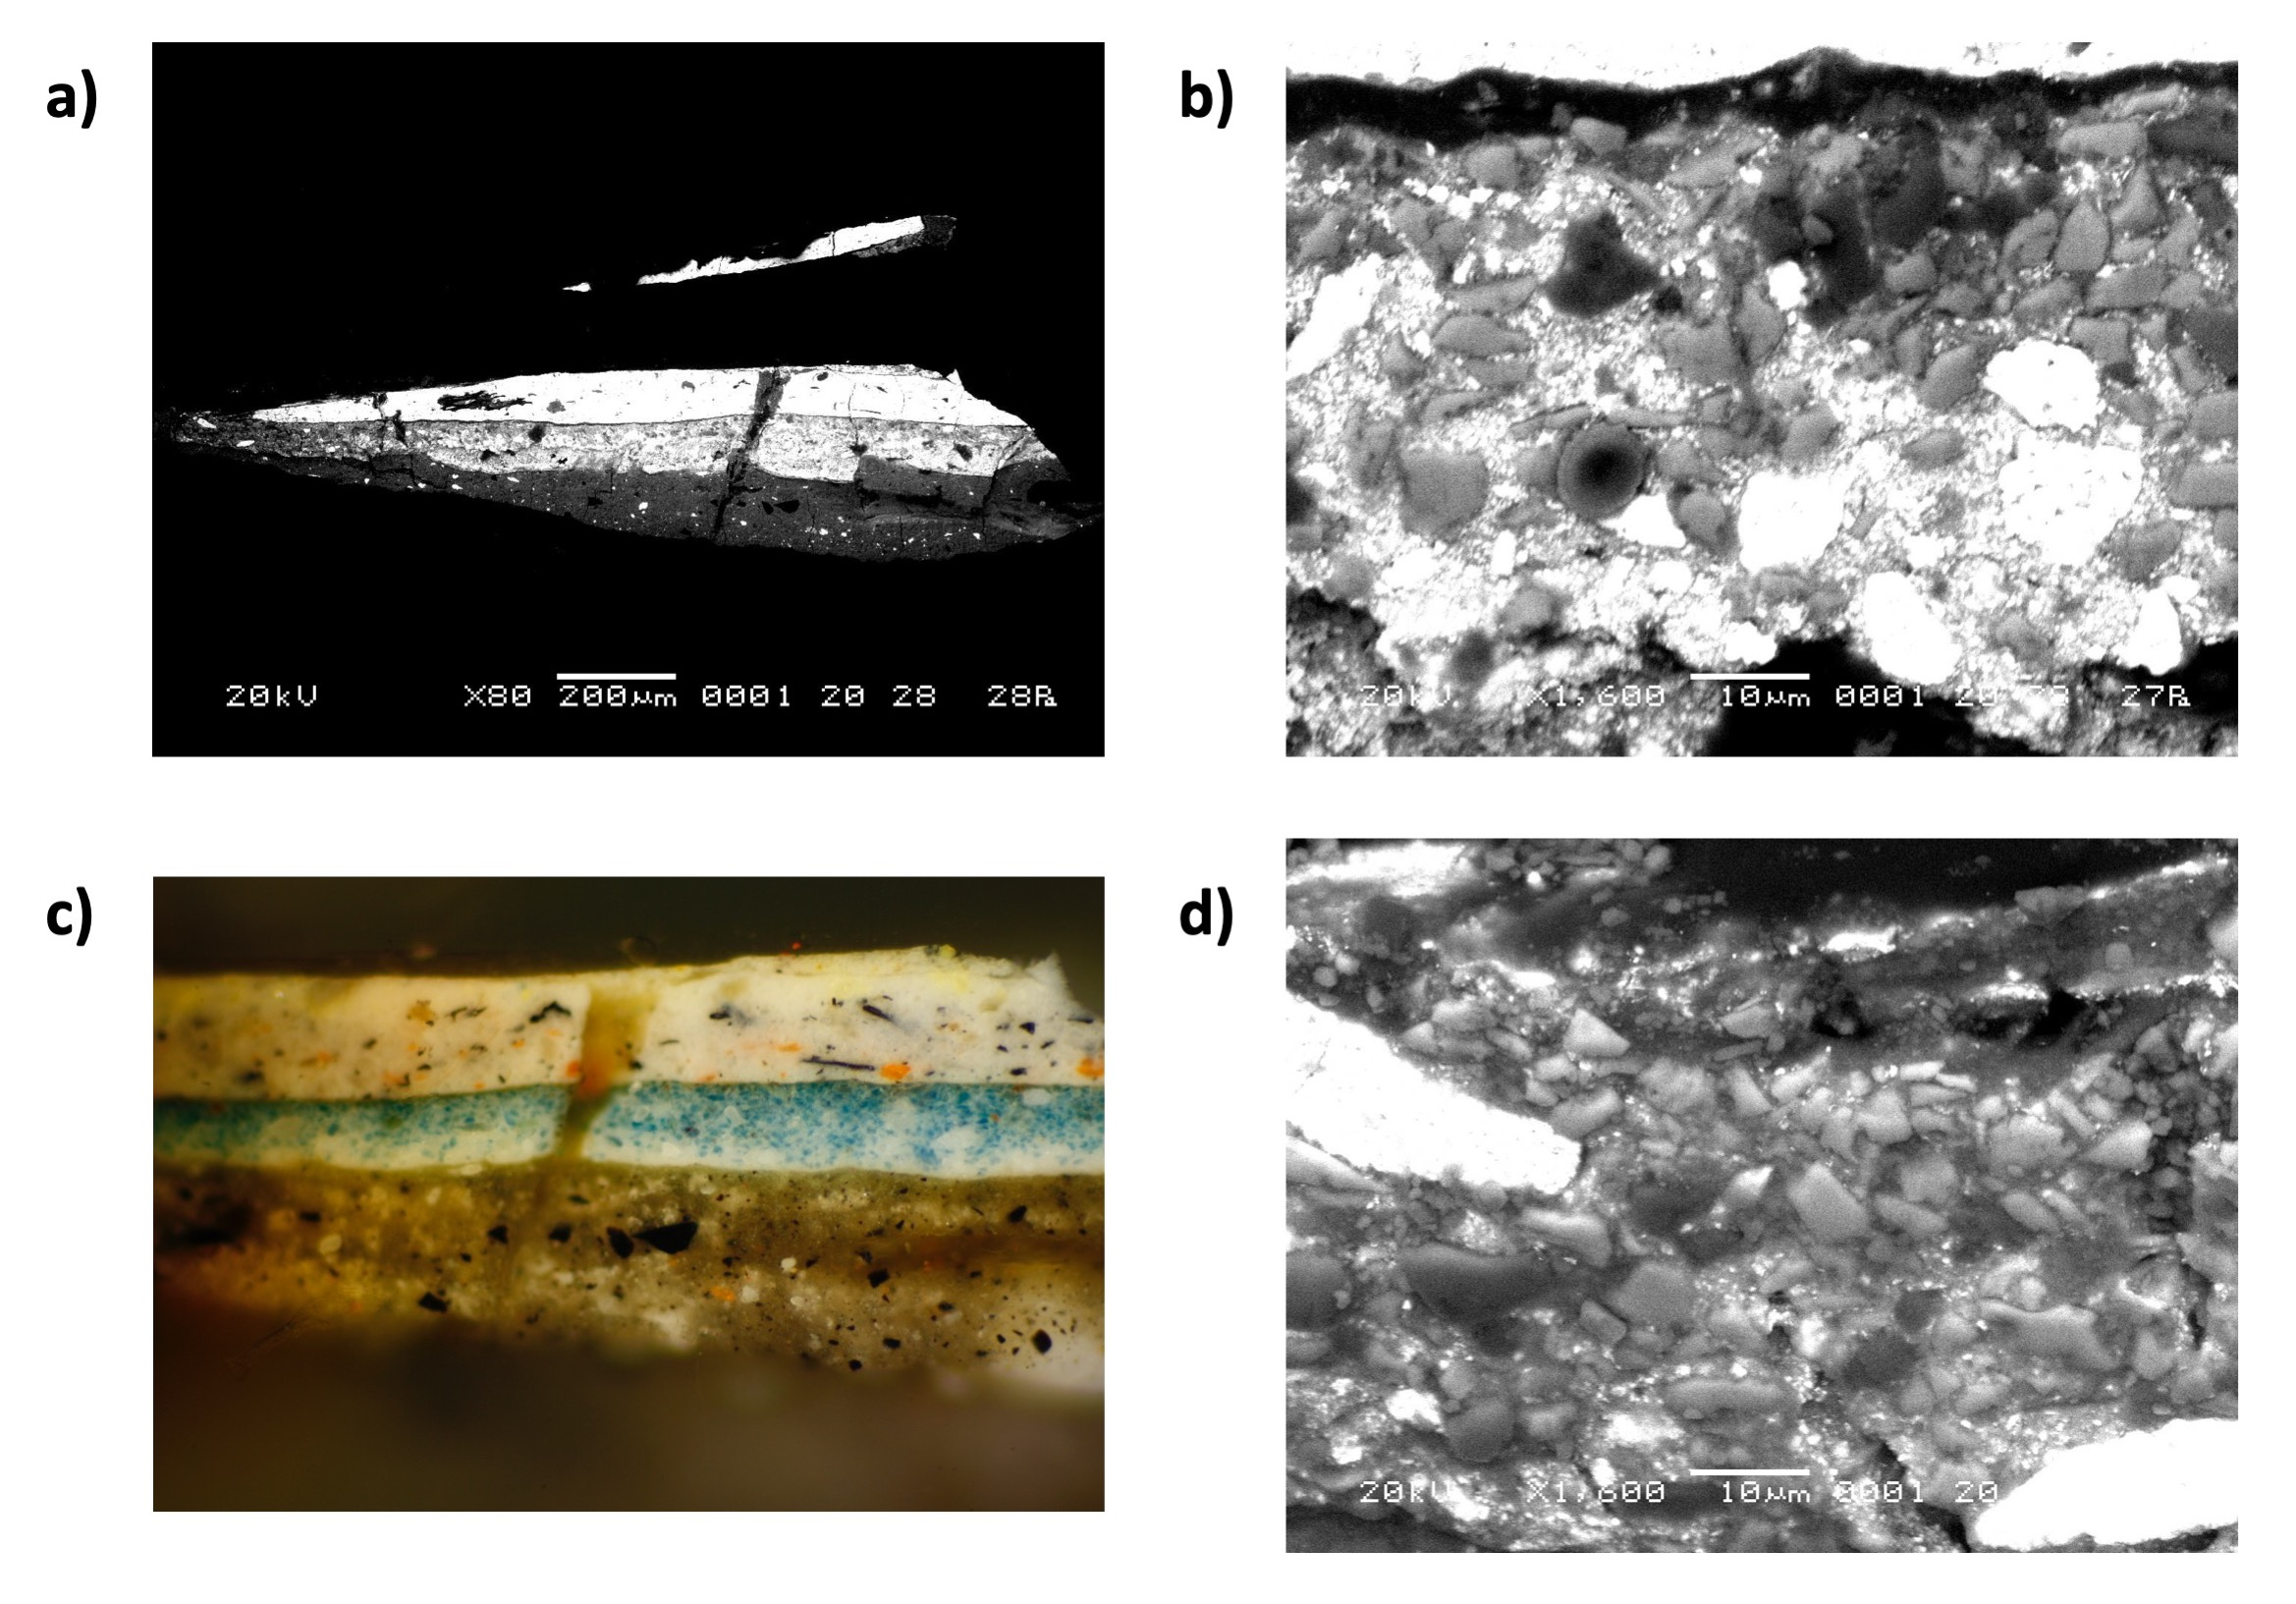
\includegraphics[width=0.8\linewidth]{1259.19_imgs}
\caption[SEM and dark-field microscope images of sample 1259.19.]{SEM and dark-field microscope images of sample 1259.19: \textbf{a)} 80x magnification, \textbf{b)} 1600x magnification, \textbf{c)} dark field microscope image provided courtesy of Katharine Waldron, HKI, \textbf{d)} 1600x magnification. The azurite containing layer shows blue and white pigments mixed together.}
\label{fig:1259.19_imgs}
\end{figure}

\begin{figure}[H]
\centering
  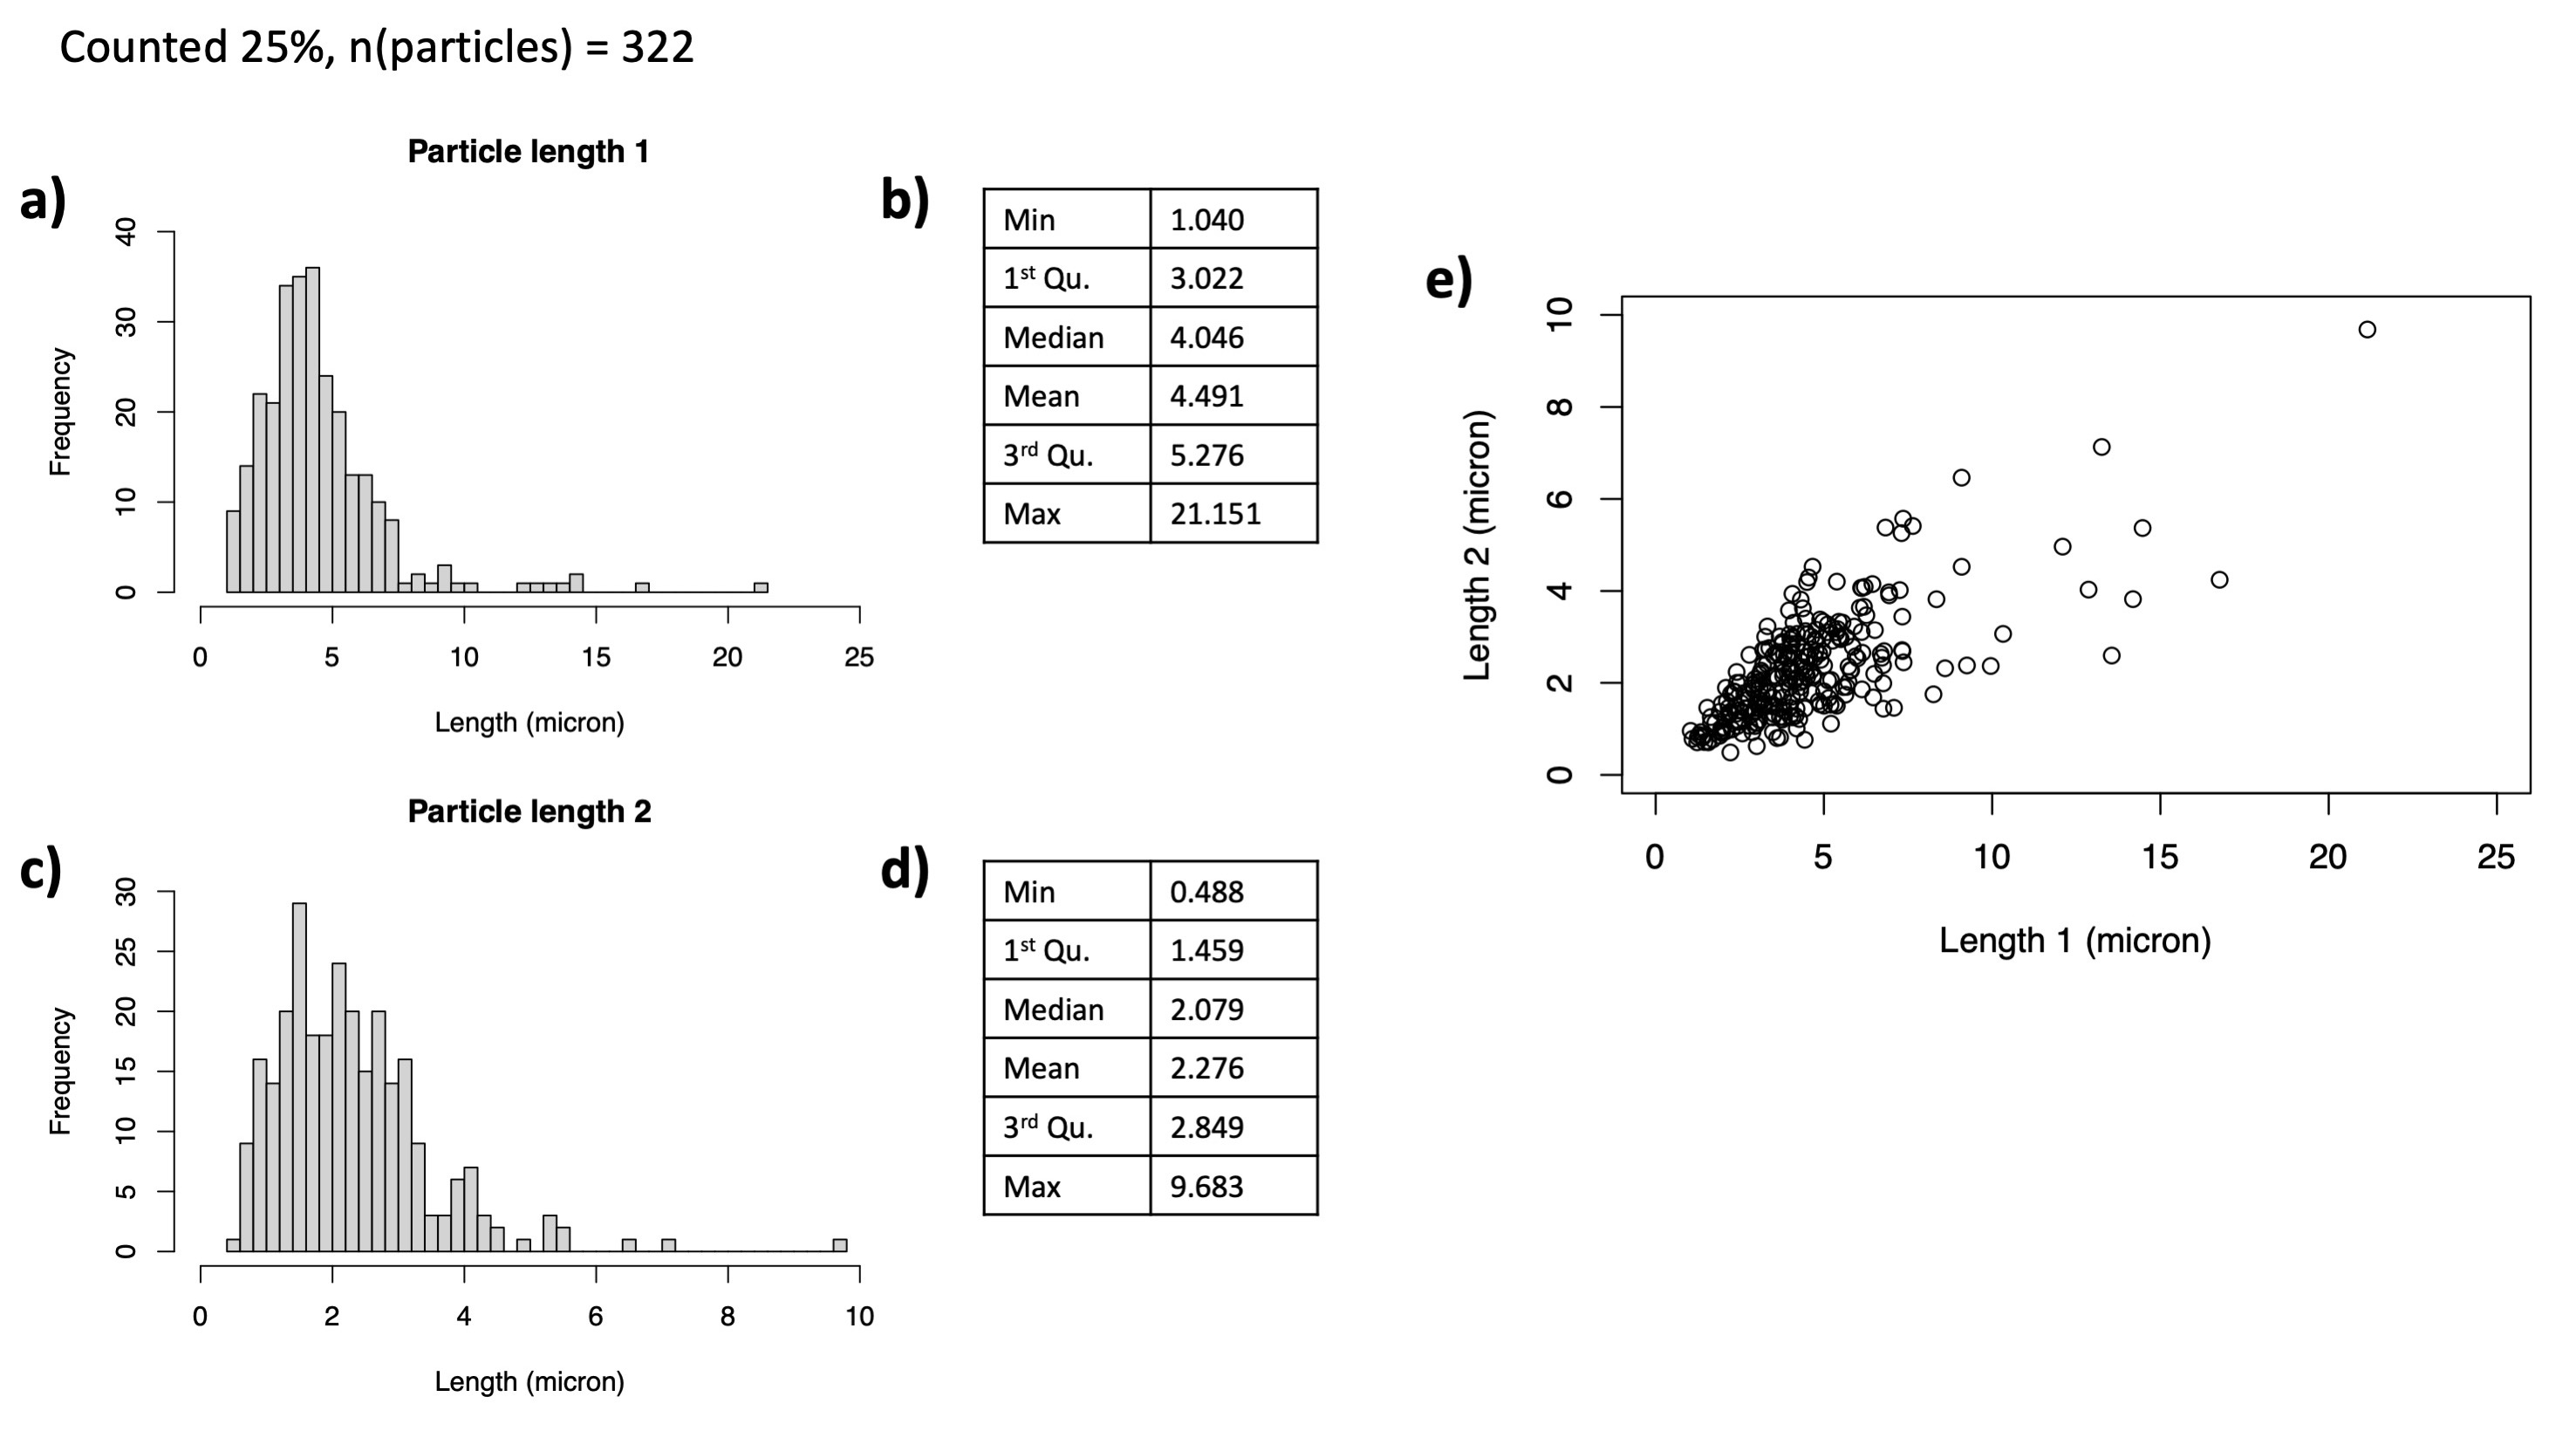
\includegraphics[width=0.8\linewidth]{1259.19_partsize}
\caption[Particle size distribution, sample 1259.19.]{Particle size distribution of sample 1259.19: \textbf{a)} Histogram showing distribution of particle length 1 values. \textbf{b)} Descriptive statistics for particle length 1 data. \textbf{c)} Histogram showing distribution of particle length 2 values. \textbf{d)} Descriptive statistics for particle length 2 data. \textbf{e)} Graph of length 1 versus length 2 showing the degree of skew.}
\label{fig:1259.19_partsize}
\end{figure}



\section{Sample 1259.20}

\begin{figure}[H]
  \centering
  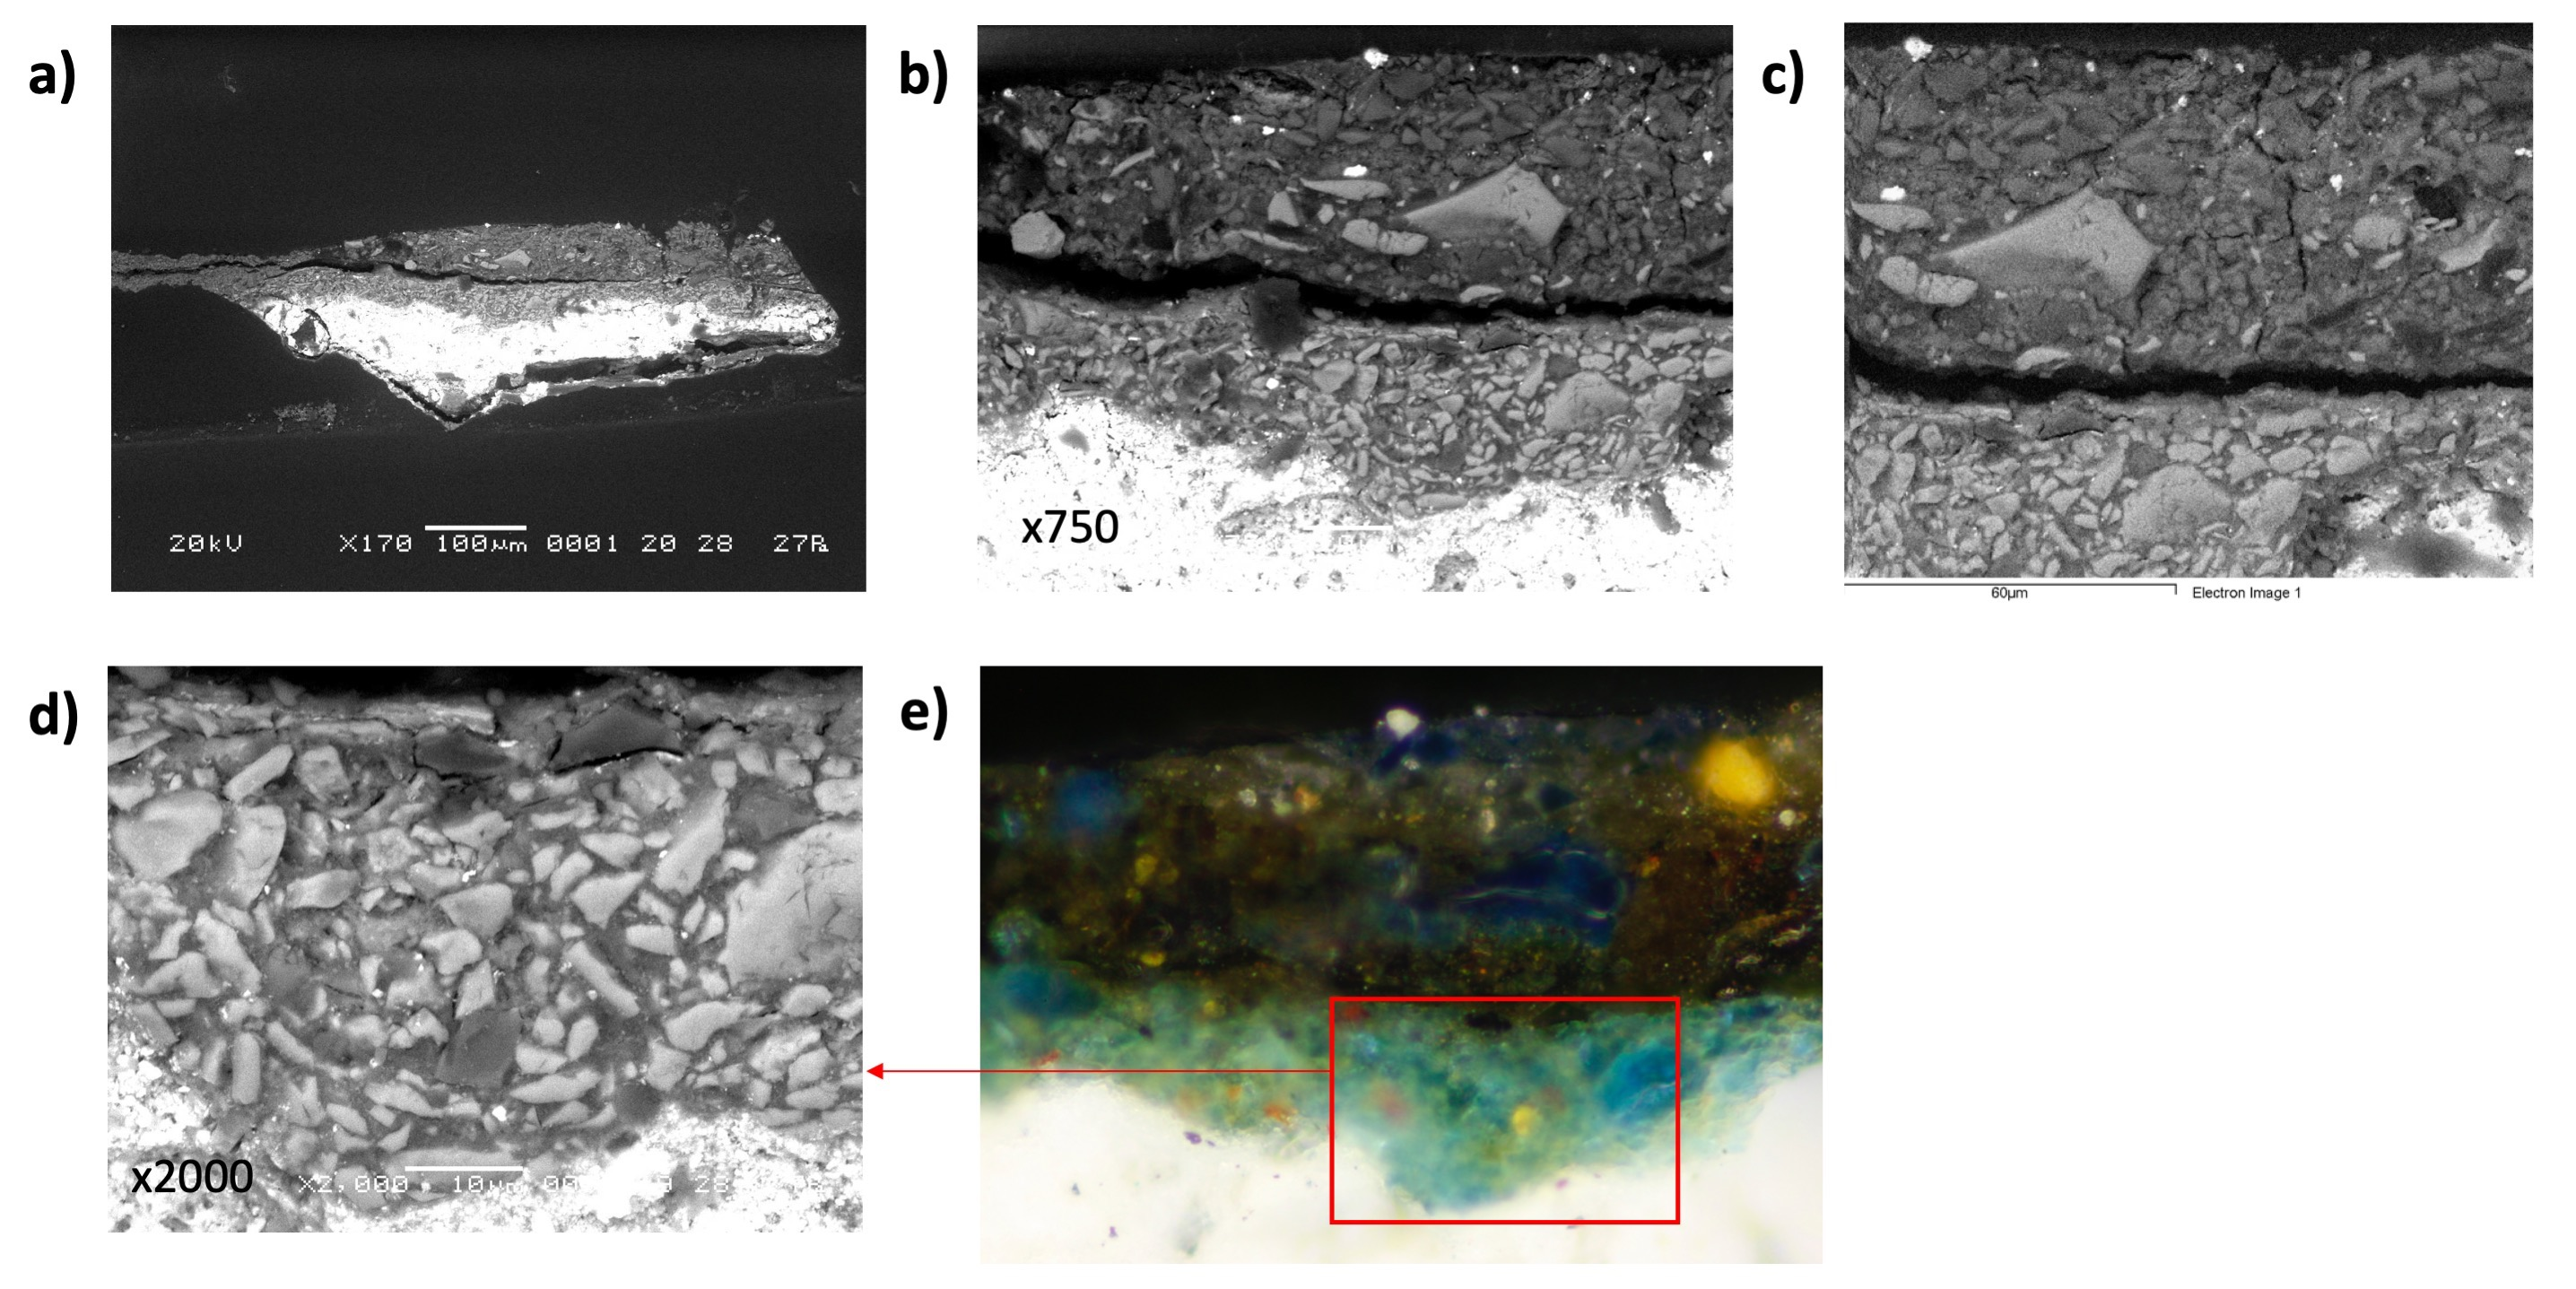
\includegraphics[width=0.8\linewidth]{1259.20_imgs}
\caption[SEM and dark-field microscope images of sample 1259.19.]{SEM and dark-field microscope images of sample 1259.19: \textbf{a)} 170x magnification, \textbf{b)} 750x magnification, \textbf{c)} 1600x magnification, \textbf{d)} 2000x magnification, \textbf{e)} dark field microscope image provided courtesy of Katharine Waldron, HKI. The area shown in \textbf{c)} is shown in the dark field image using a red box. Darker blue overpaint layers are modern, though azurite is also used.}
\label{fig:1259.20_imgs}
\end{figure}

Areas of visible blue particles in overpaint of sample 1259.20 were studied by confocal Raman spectroscopy to confirm their identity as azurite. An example sample spectrum is shown in \textit{Figure \ref{fig:raman_1259-20}}. Although the sample spectra suffer from low intensities compared to fluorescence from the surrounding resin, the characteristic band at 400 cm\textsuperscript{-1} is visible, confirming the presence of azurite.

\begin{figure}[H] 
\centering
  \includegraphics[width=0.8\linewidth]{1259.20_blue_overpaint}
\caption[Raman spectral data, 1259.20]{Raman spectral data: sample 1259.20. An azurite reference spectrum (blue line) is shown as a comparison to sample 1259.20 (red circles). The spectral data from 1259.20 is smoothed using an FFT filter (black line). Spectra are off-set for clarity.}
\label{fig:raman_1259-20}
\end{figure}

\begin{figure}[H]
\centering
\begin{minipage}[t]{\linewidth}
  \centering
  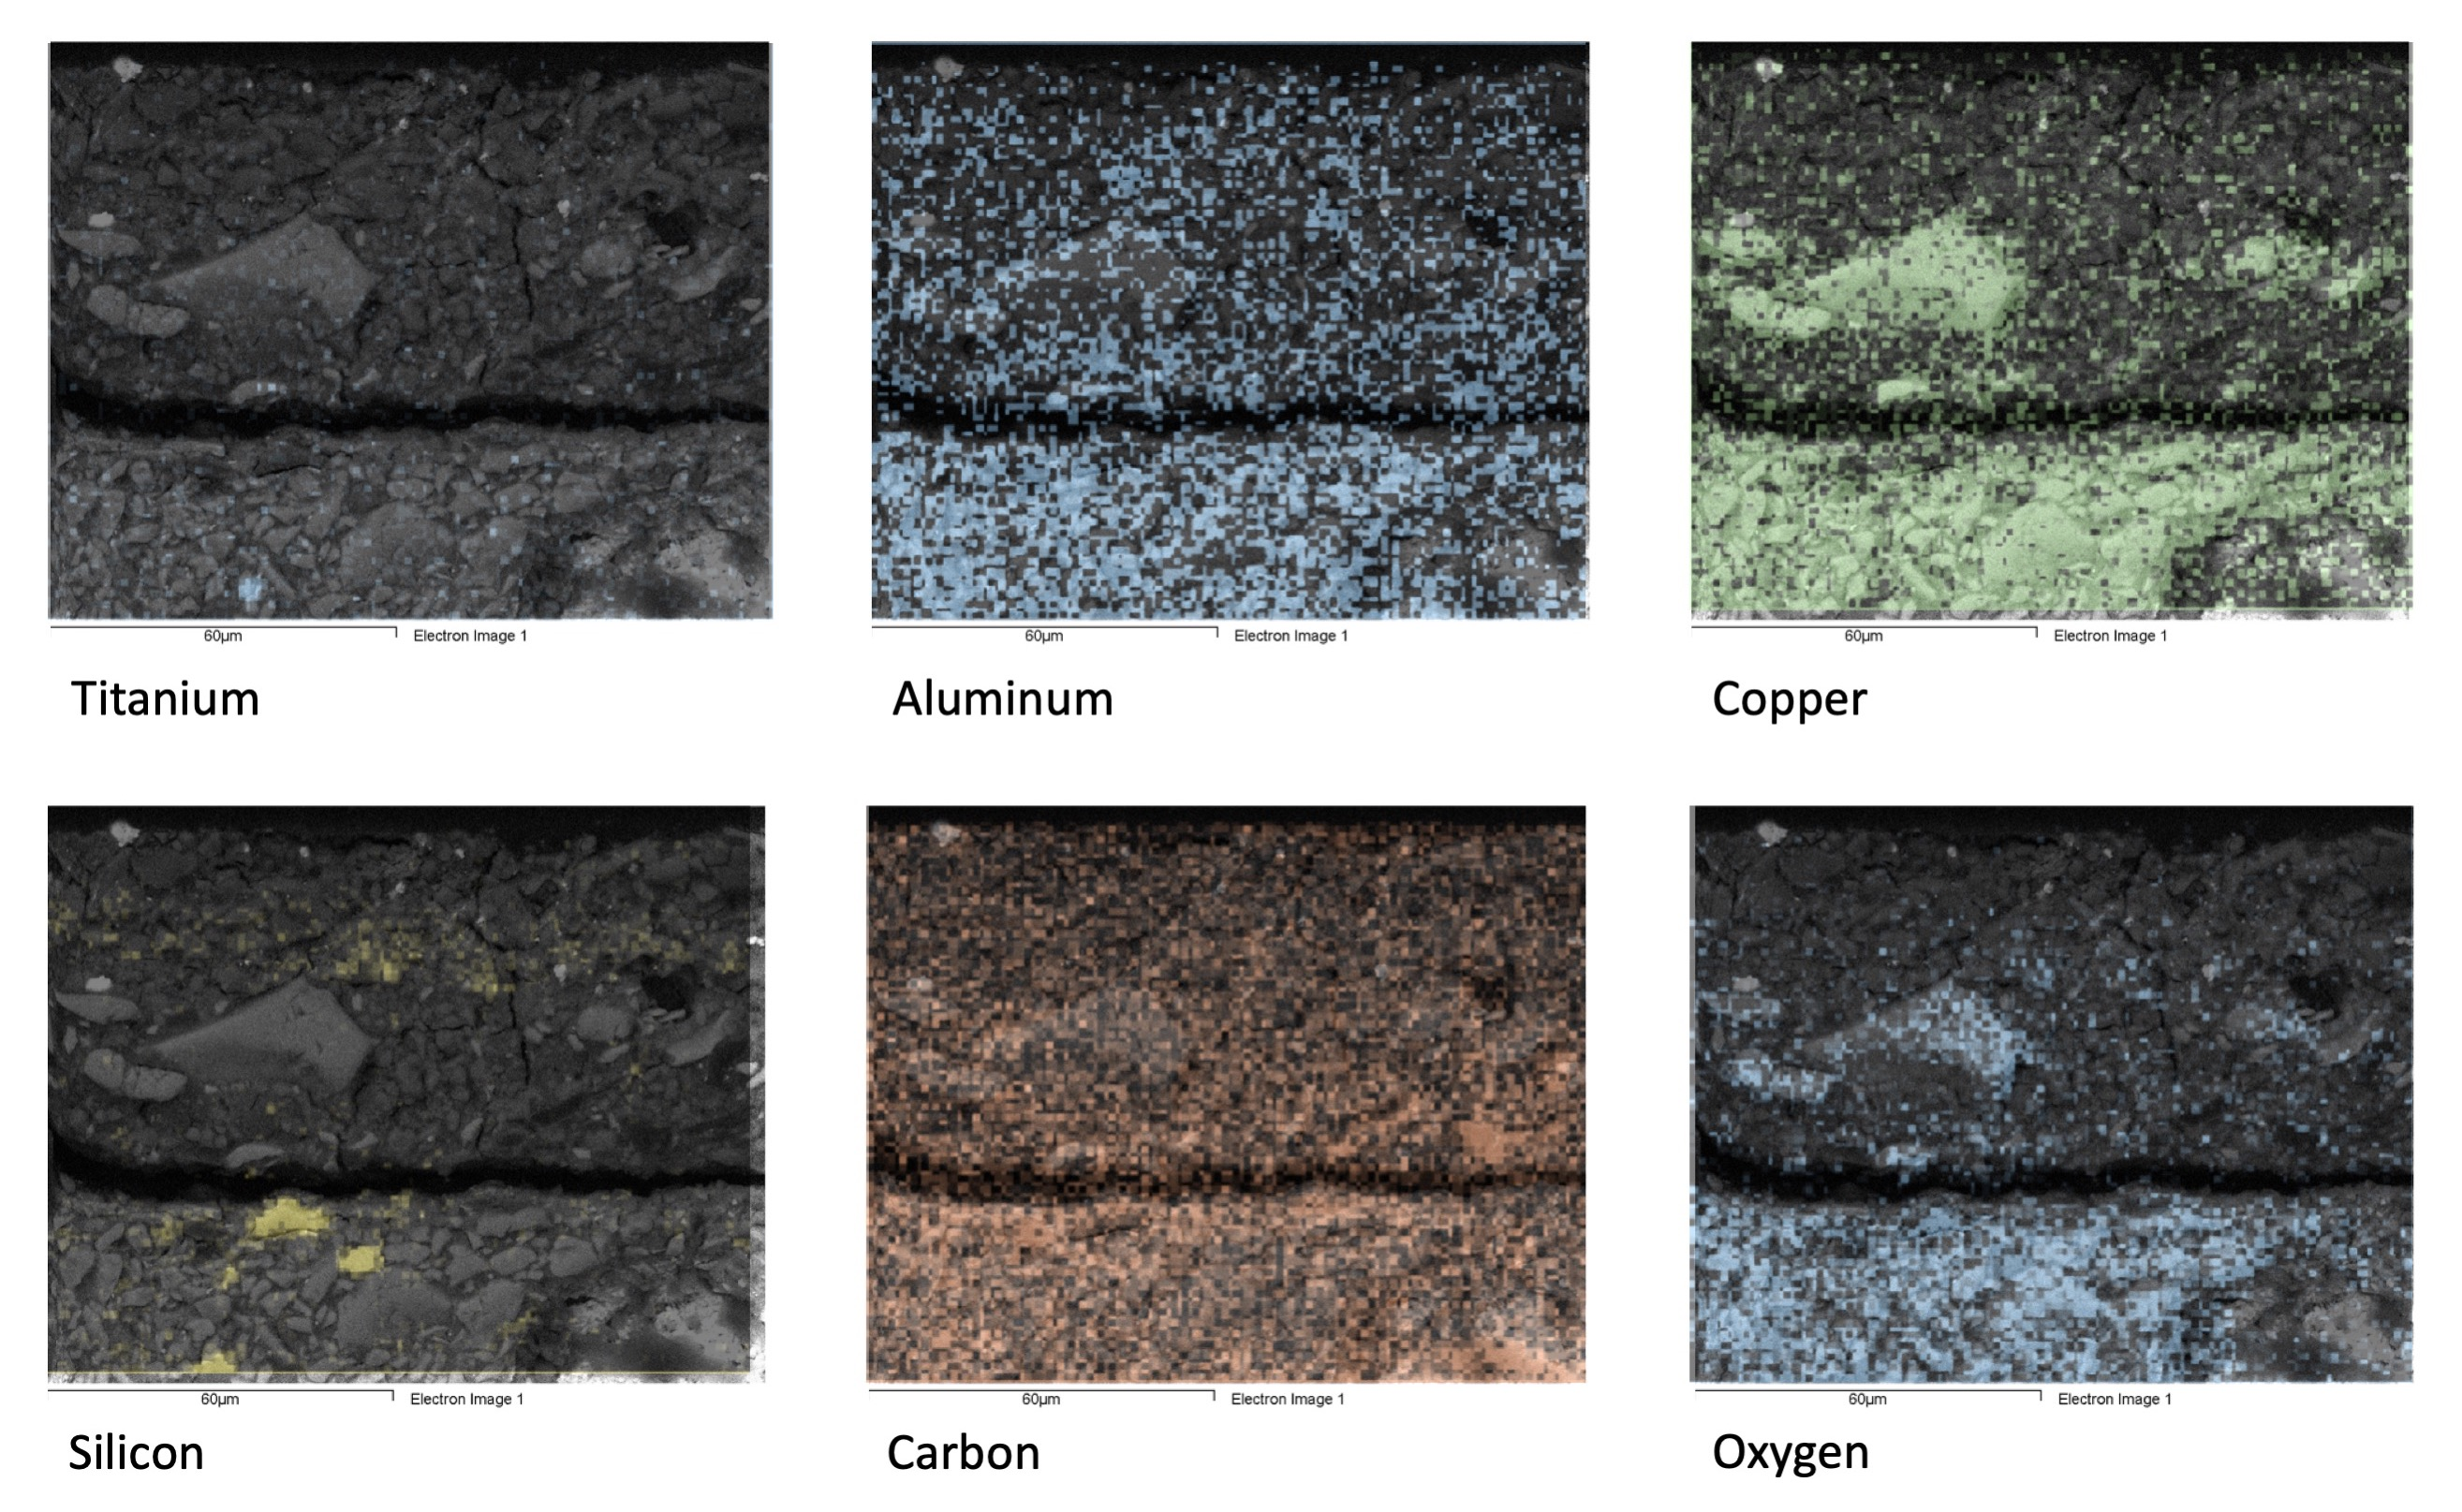
\includegraphics[width=0.9\linewidth]{1259.20_mapdata_1}
\hfill
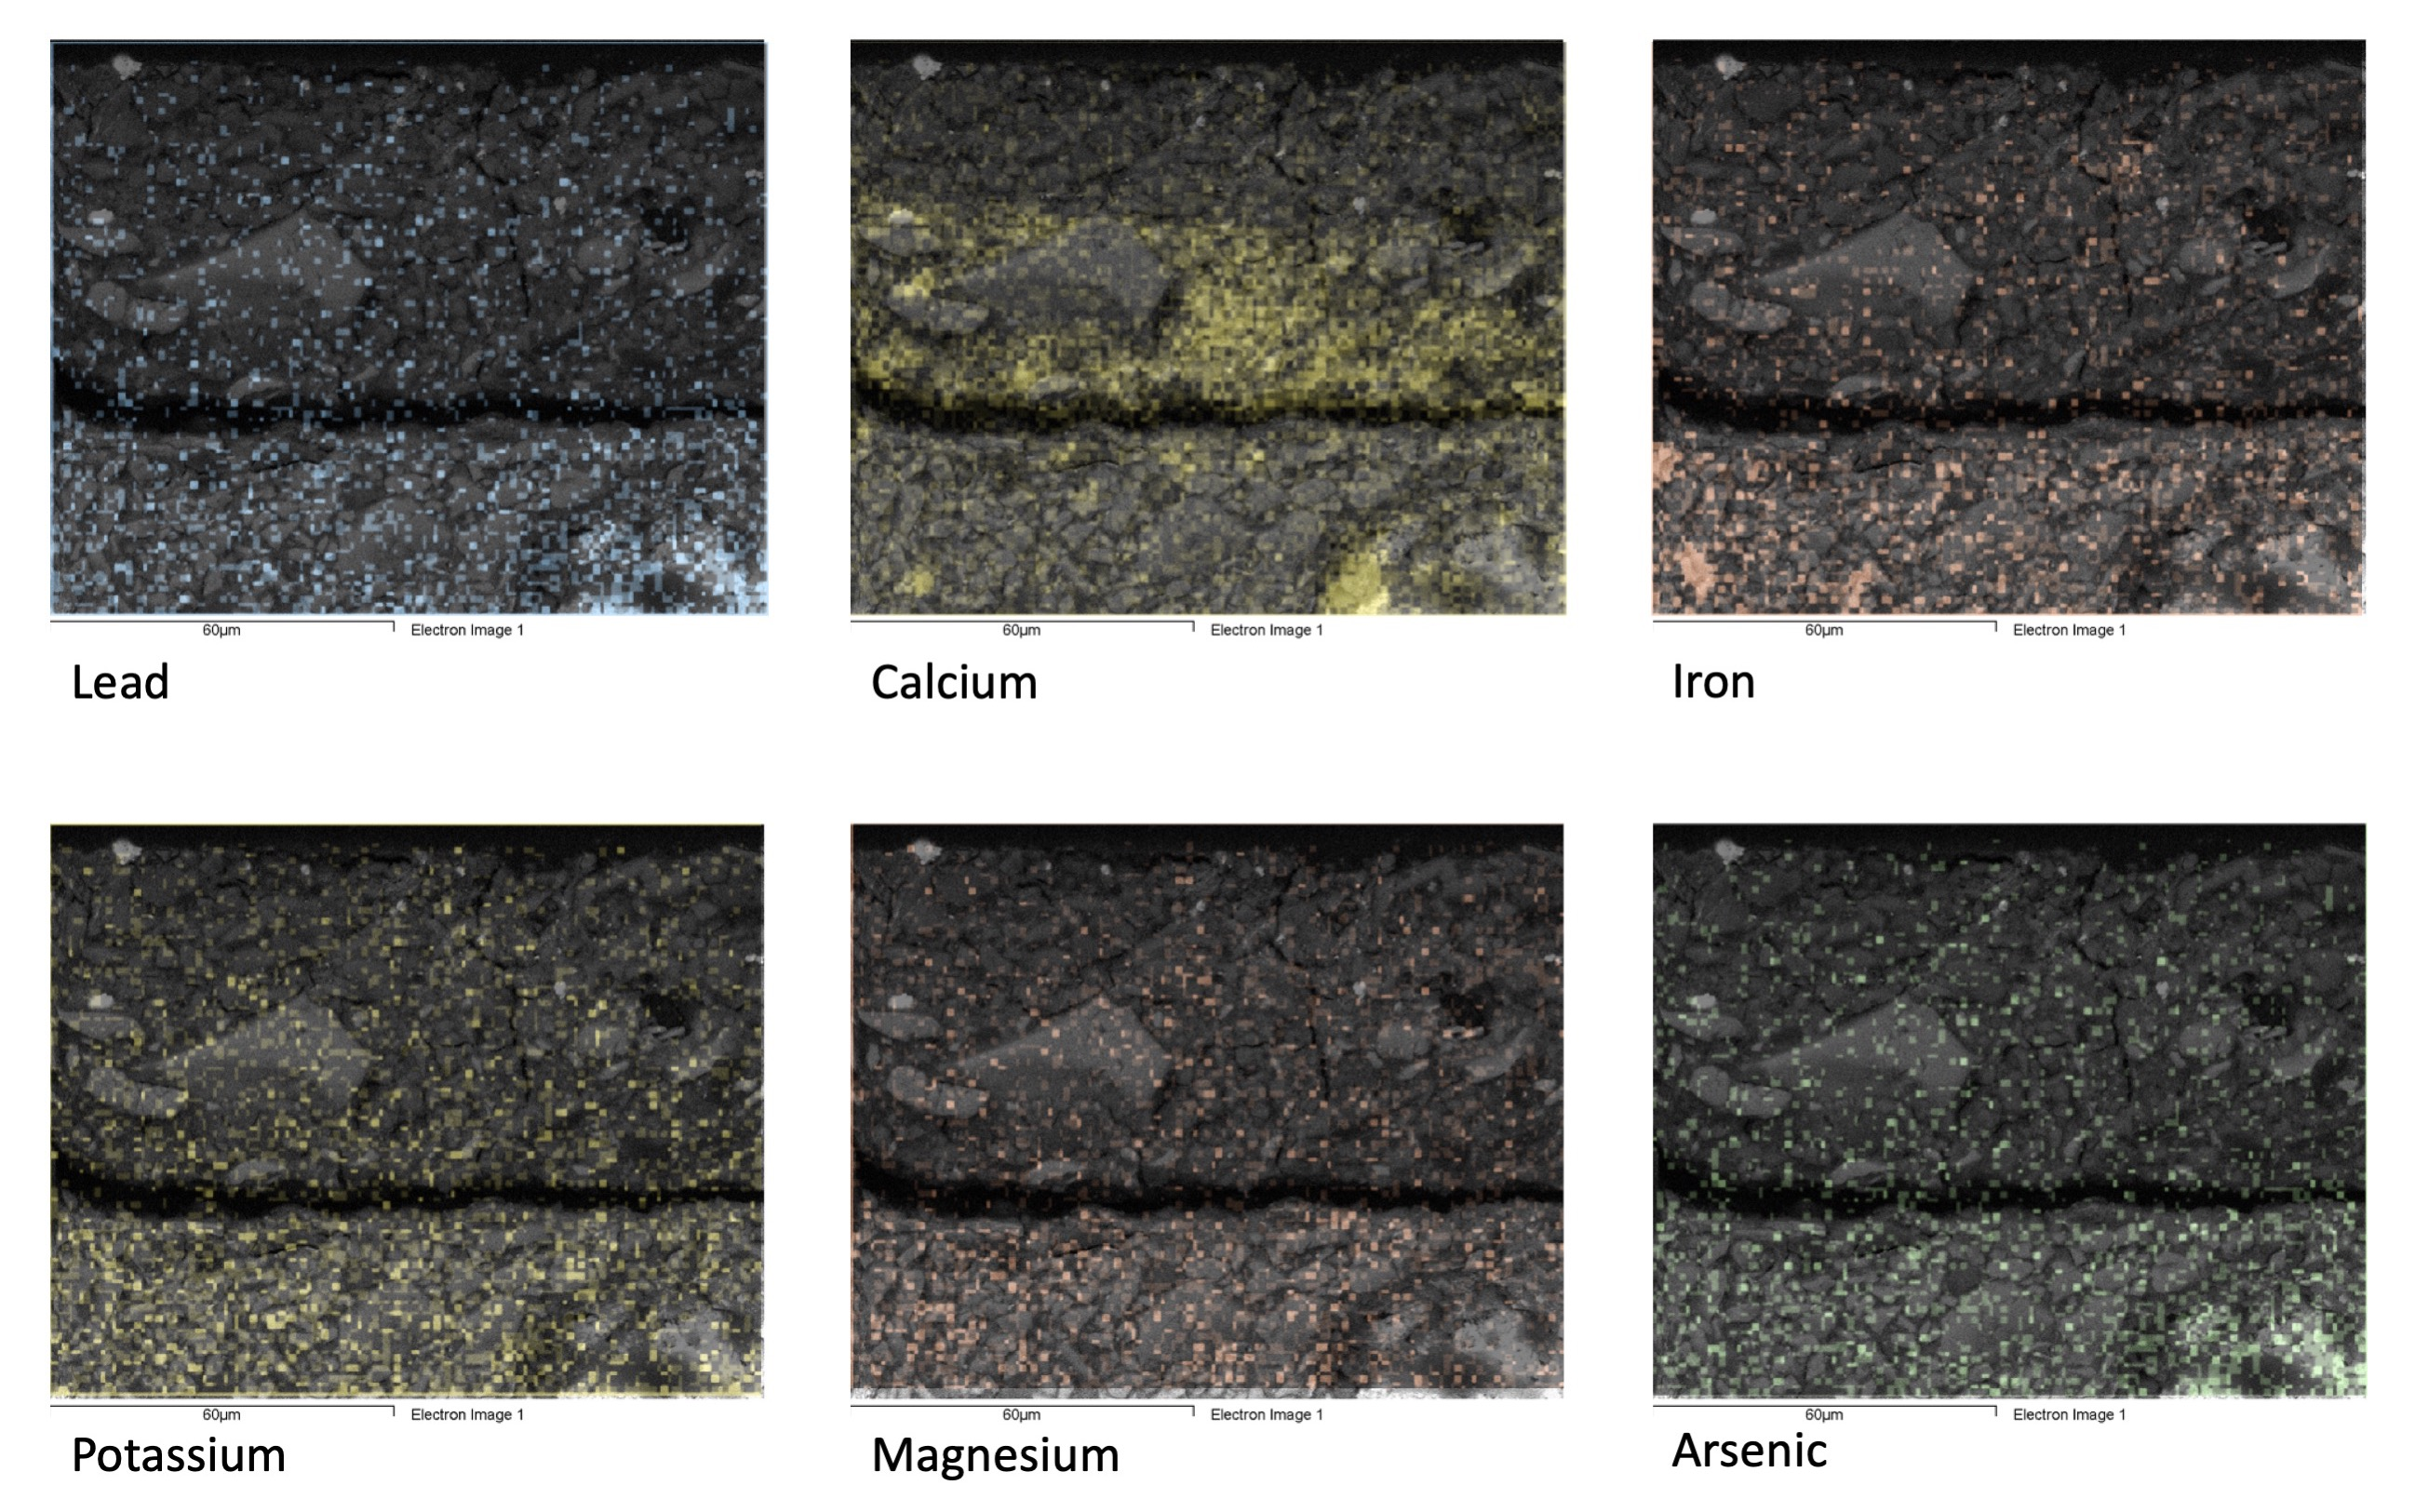
\includegraphics[width=0.9\linewidth]{1259.20_mapdata_2}
\hfill
\end{minipage}
\caption[EDS map data, sample 1259.20.]{EDS map data of sample 1259.20 showing locations of elements in an area of the azurite paint layer. Elements detected are Ti, Al, Cu, Si, C, O, Pb, Ca, Fe, K, Mg, and As.}
\label{fig:1259.20_mapdata}
\end{figure}

\begin{figure}[H]
\centering
  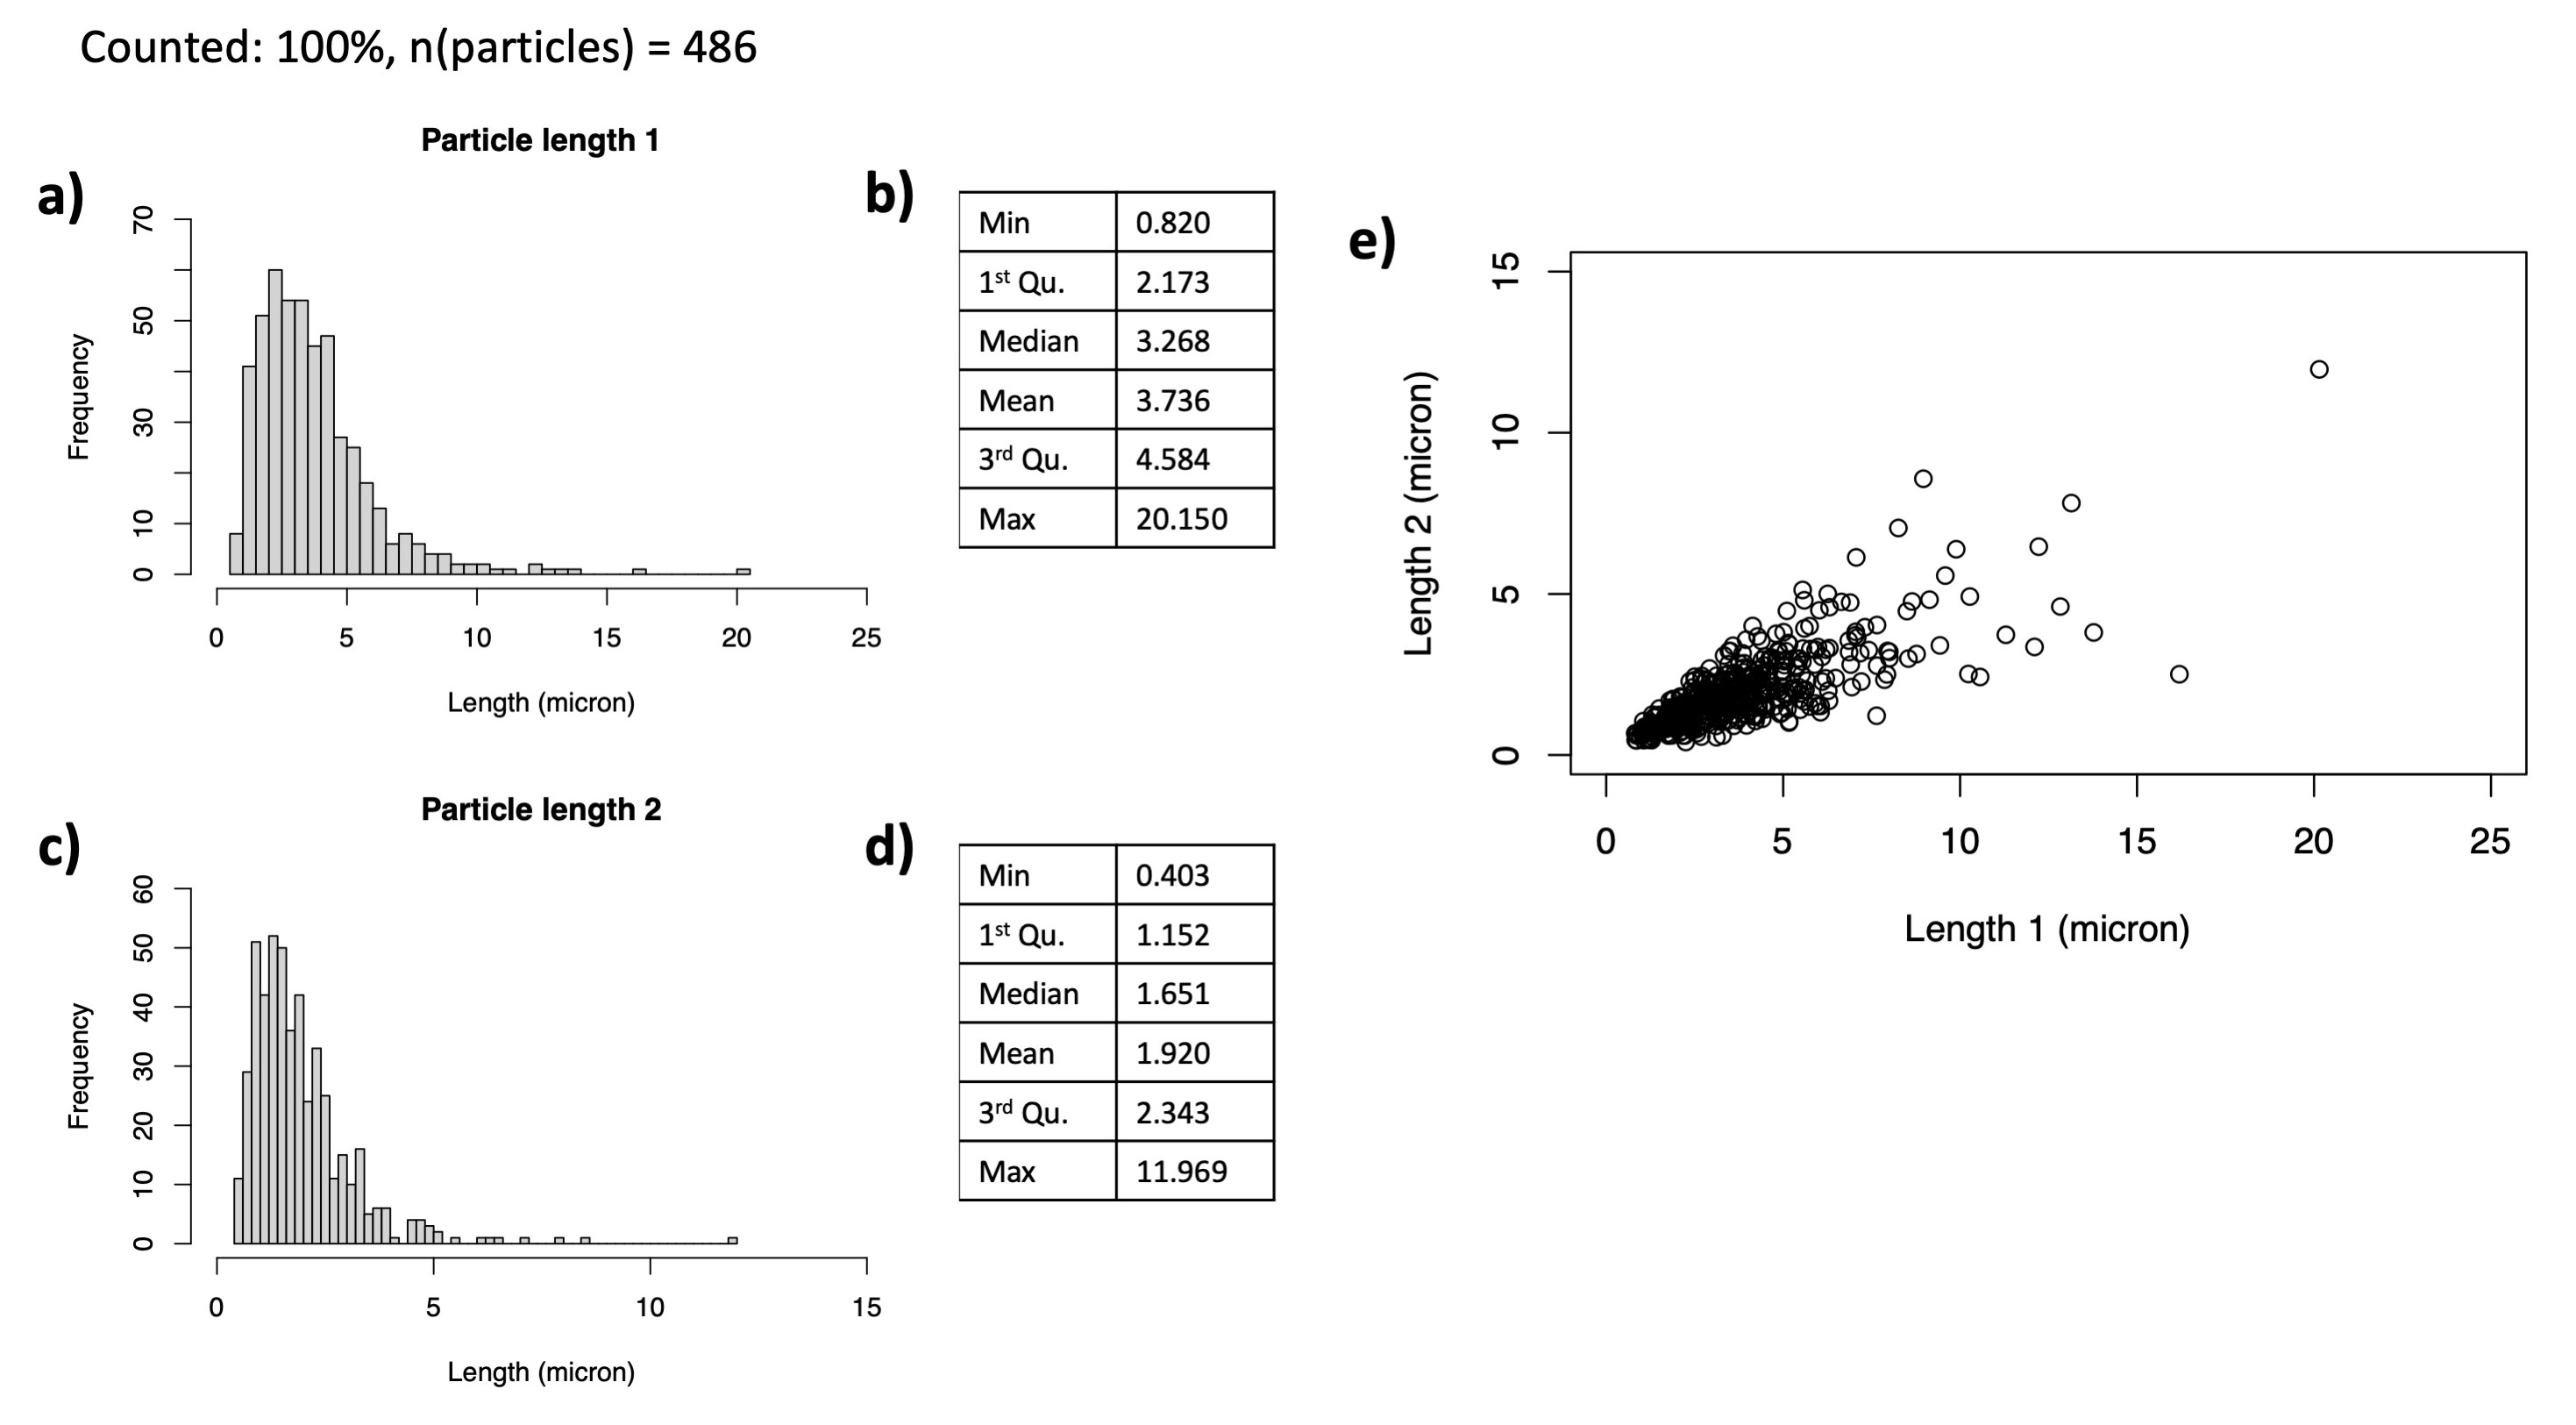
\includegraphics[width=0.8\linewidth]{1259.20_partsize}
\caption[Particle size distribution, sample 1259.20.]{Particle size distribution of sample 1259.20: \textbf{a)} Histogram showing distribution of particle length 1 values. \textbf{b)} Descriptive statistics for particle length 1 data. \textbf{c)} Histogram showing distribution of particle length 2 values. \textbf{d)} Descriptive statistics for particle length 2 data. \textbf{e)} Graph of length 1 versus length 2 showing the degree of skew.}
\label{fig:1259.20_partsize}
\end{figure}



\section{Sample 1259.21}


\begin{figure}[H]
  \centering
  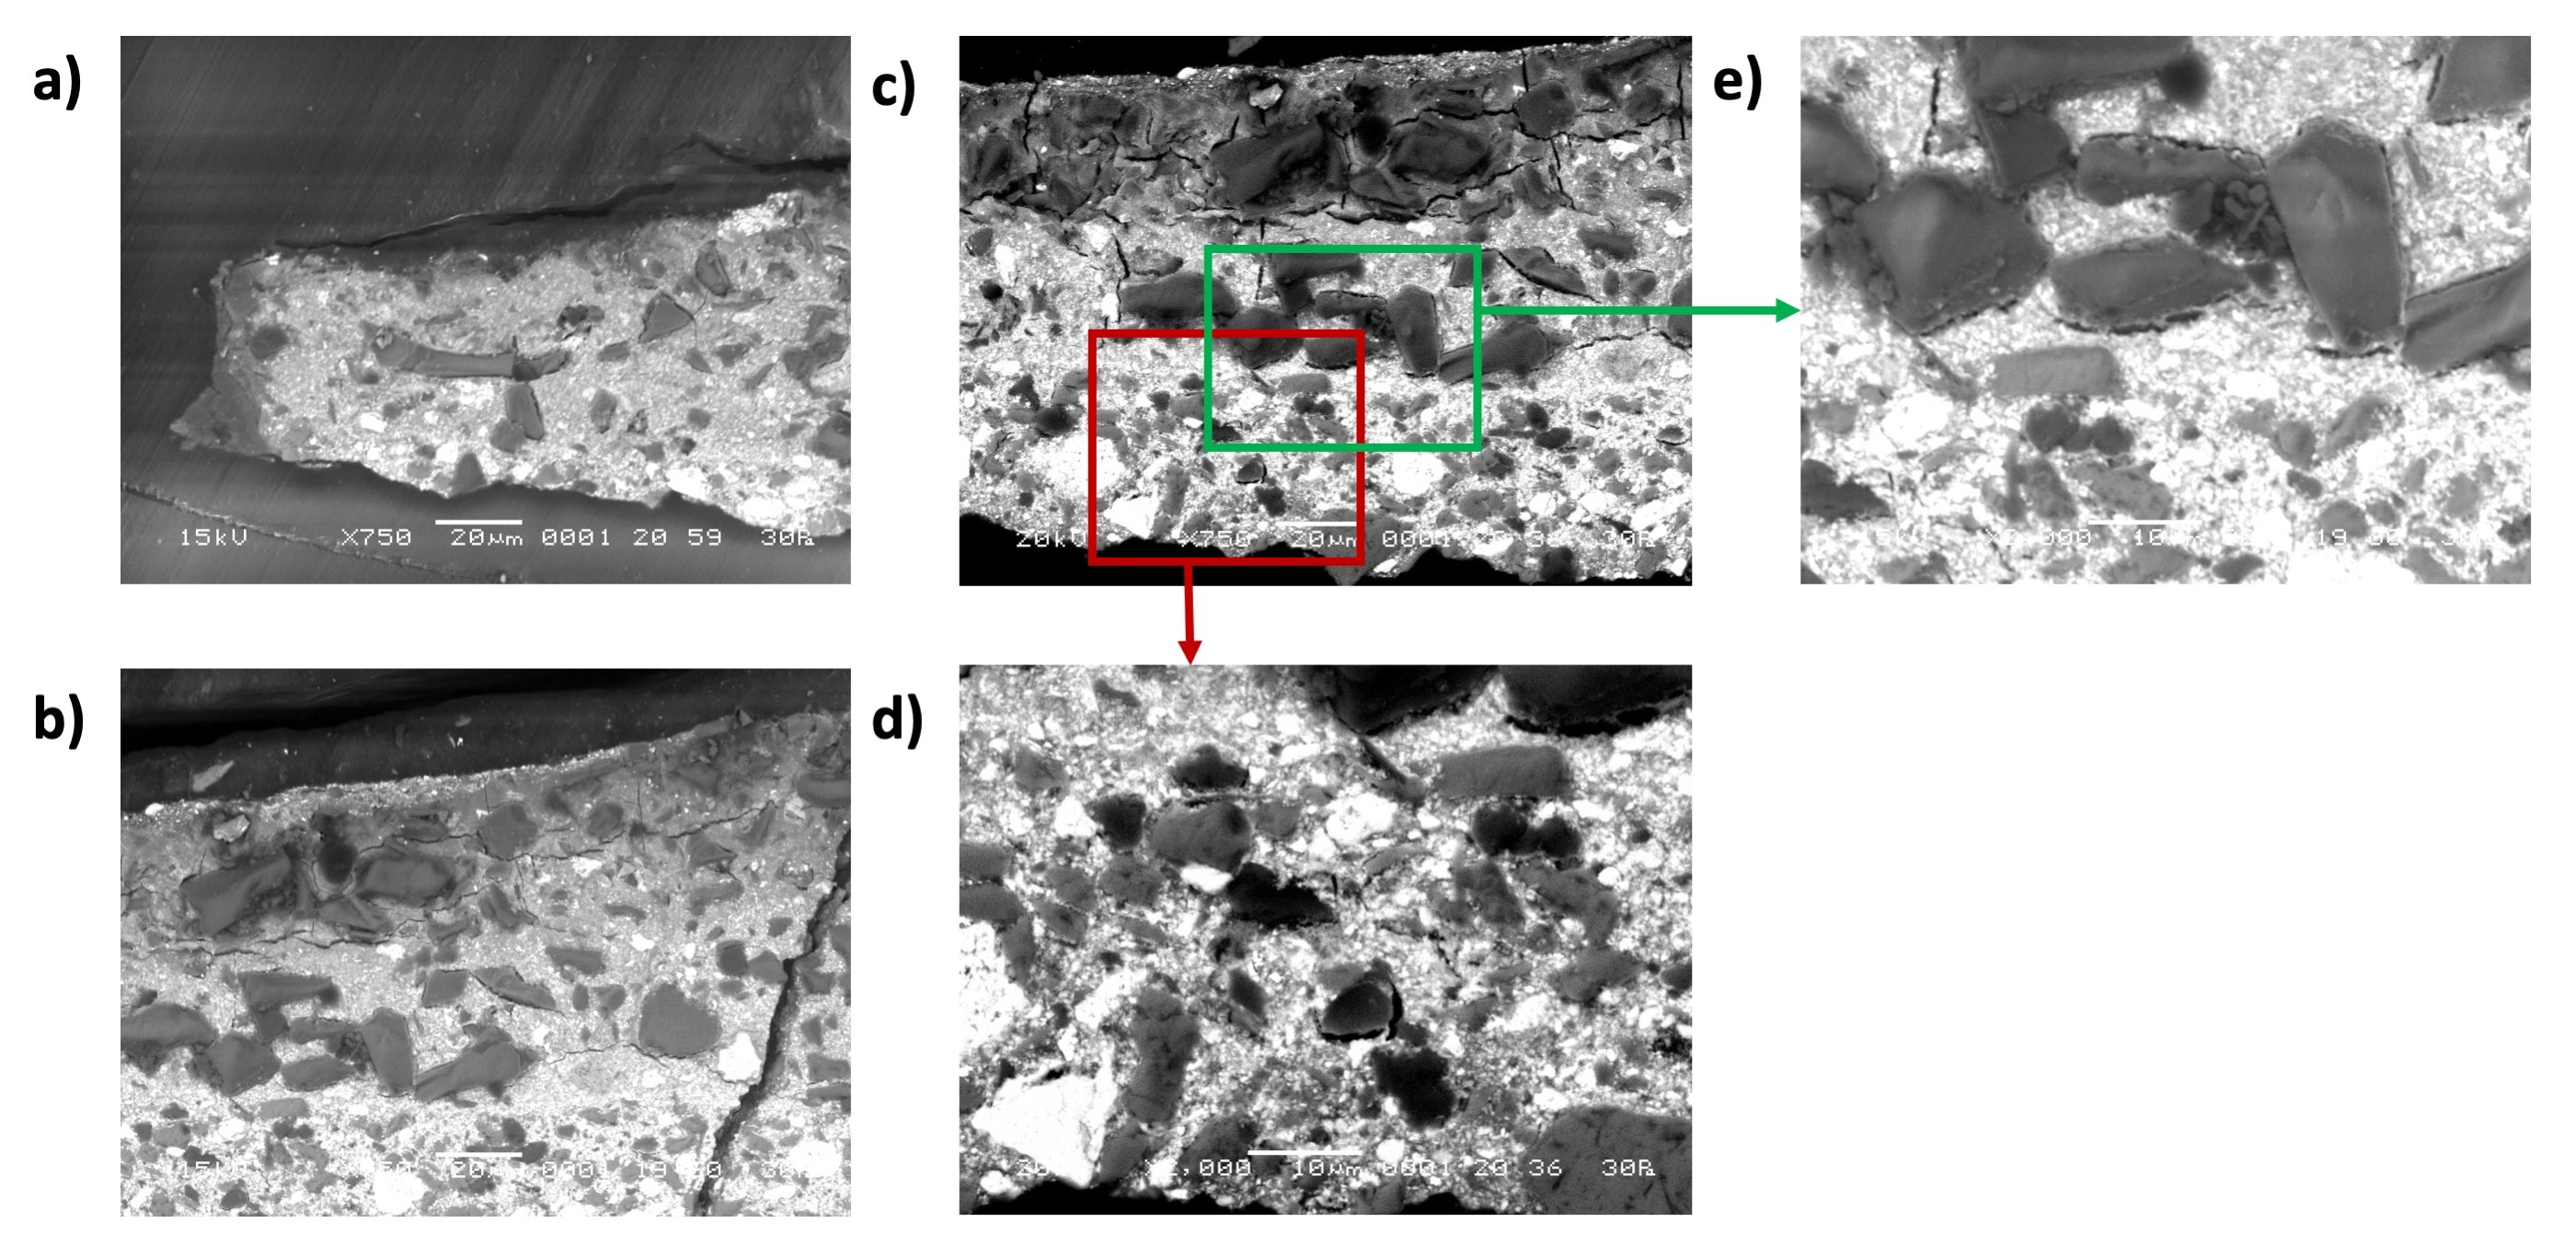
\includegraphics[width=0.8\linewidth]{1259.21_imgs}
\caption[SEM images of sample 1259.21.]{SEM images of sample 1259.21: \textbf{a)} 750x magnification, \textbf{b)} 750x magnification, \textbf{c)} 750x magnification, \textbf{d)} 2000x magnification, \textbf{e)} 2000x magnification. Red and green boxes show the areas of \textbf{c} corresponding to images \textbf{d} and \textbf{e}.}
\label{fig:1259.21_imgs}
\end{figure}

\begin{figure}[H]
  \centering
  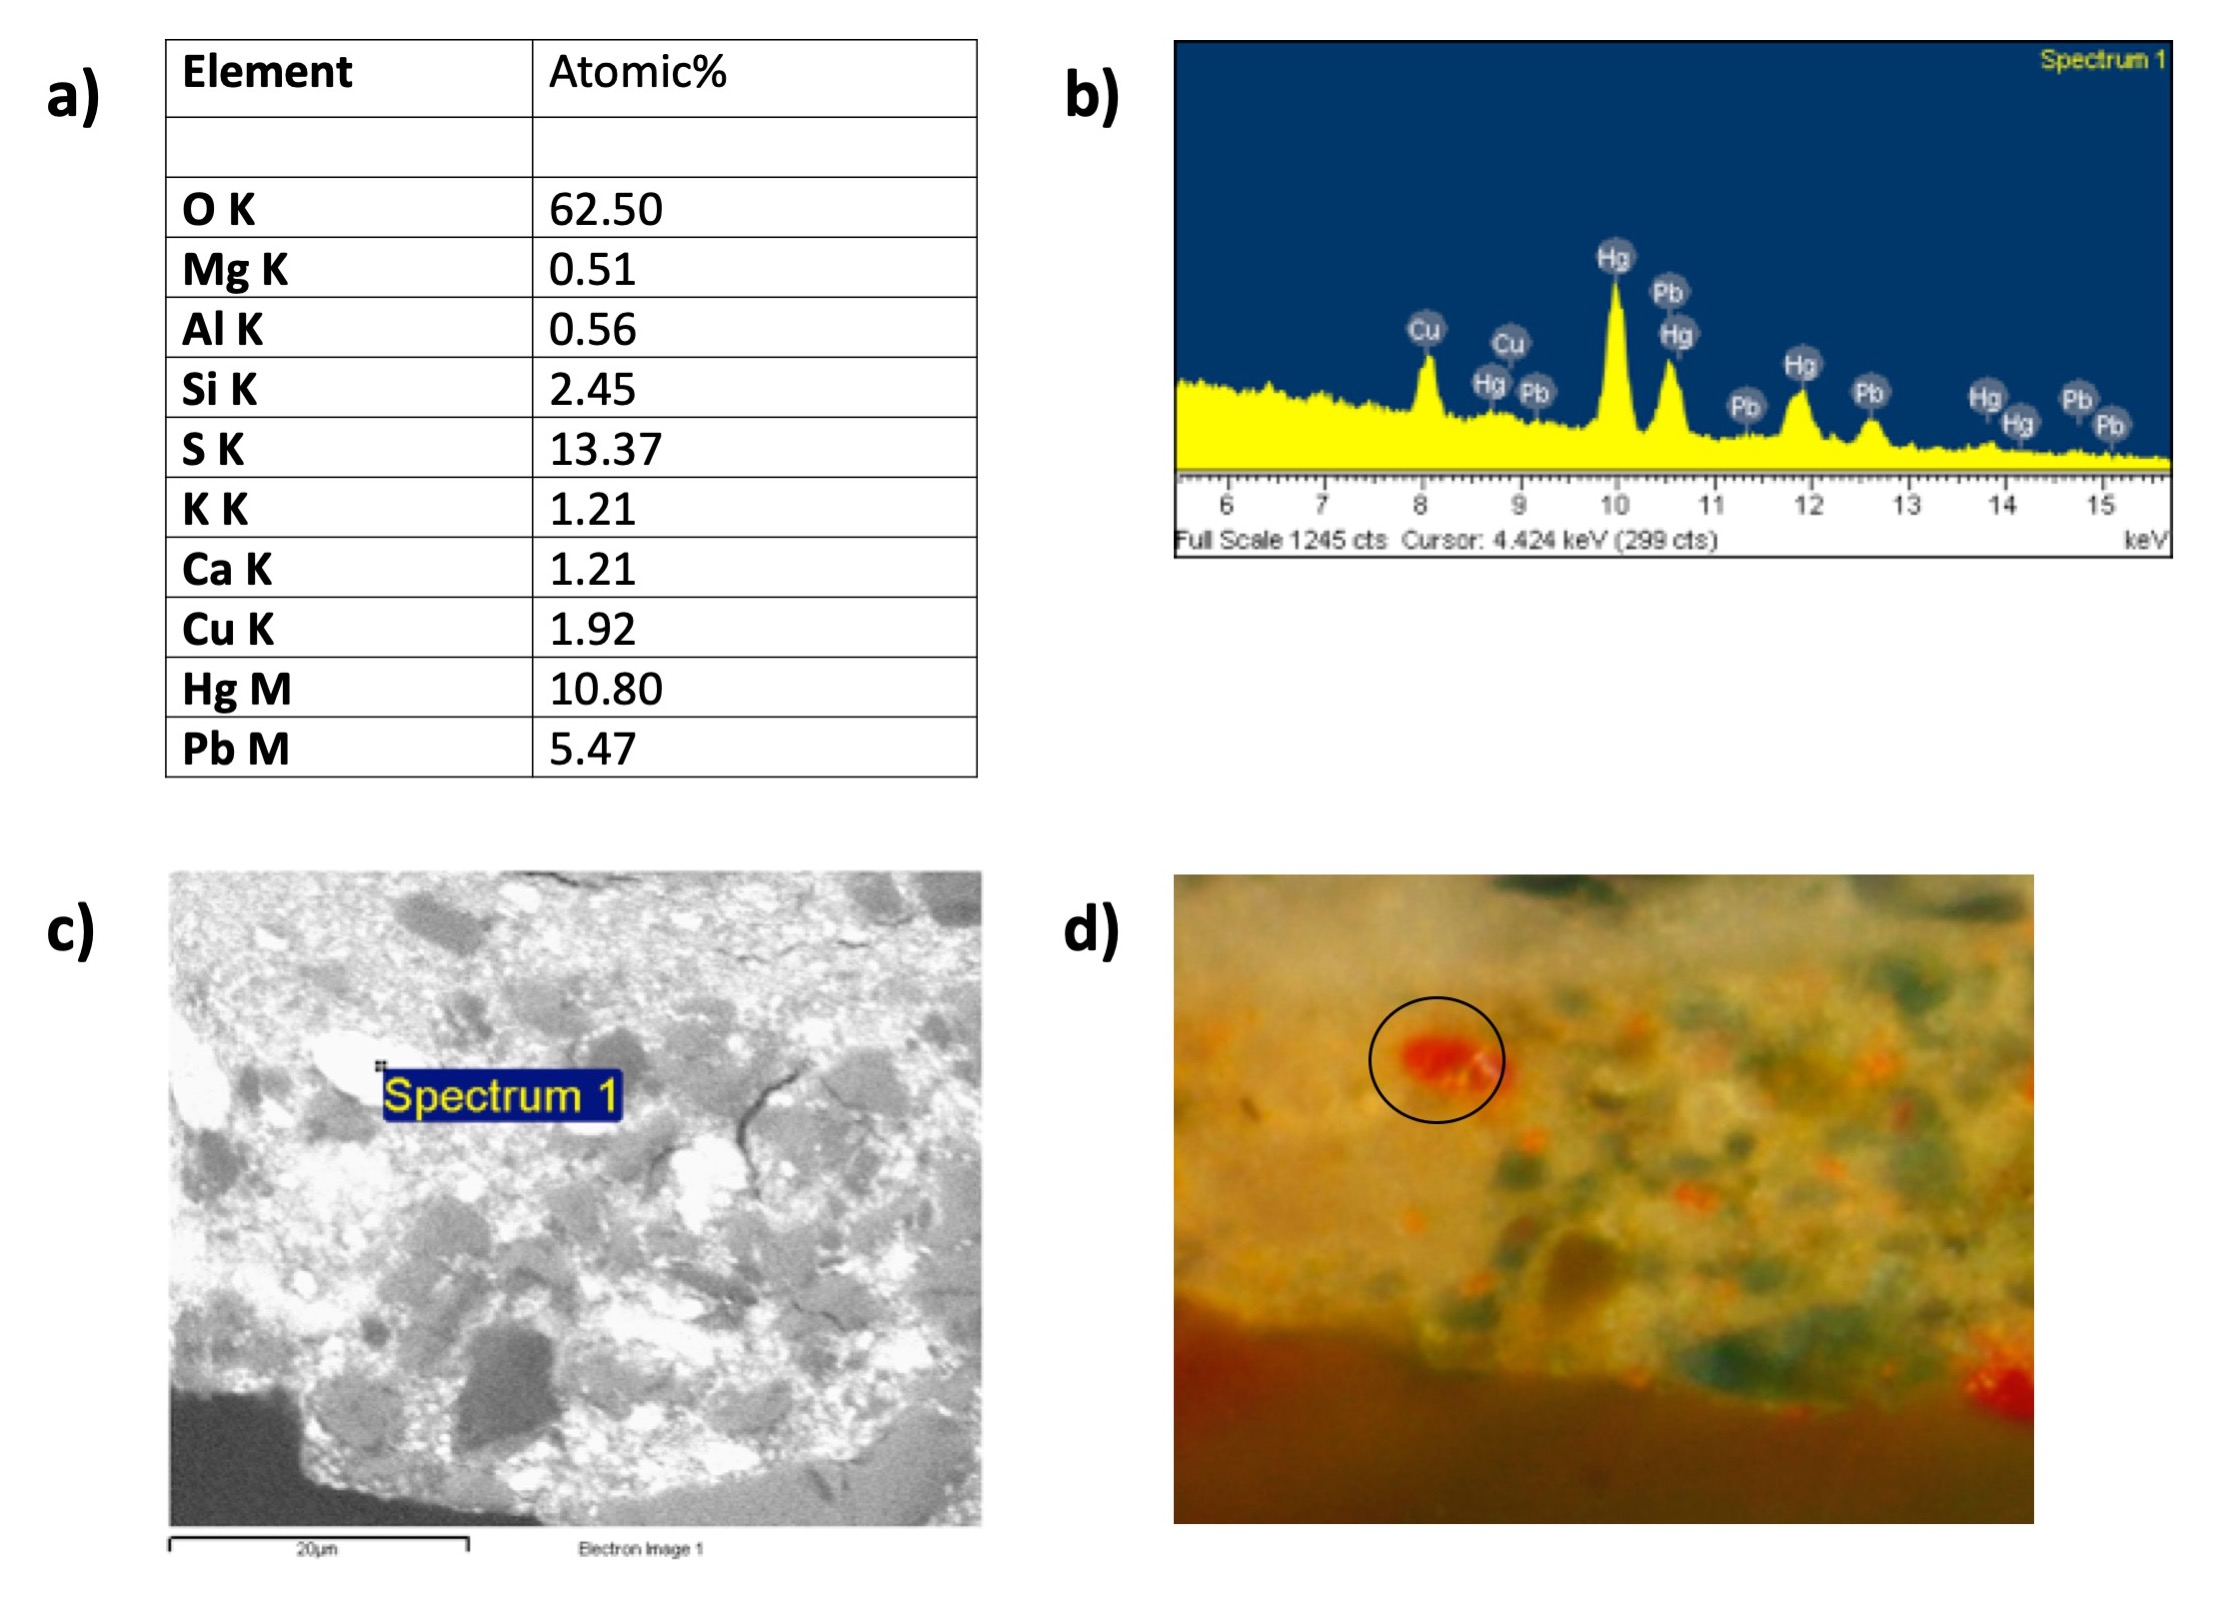
\includegraphics[width=0.8\linewidth]{1259.21_pointspec}
\caption[EDS point spectrum data, sample 1259.21.]{EDS point spectrum data, sample 1259.21: \textbf{a)} Quantitative EDS results of red pigment particle showing high levels of mercury and sulfur, \textbf{b)} Detail area of EDS spectrum showing detection of mercury and sulfur, \textbf{c)} SEM image showing point spectrum location, \textbf{d)} dark field microscope image showing point spectrum sample location. Image is provided courtesy of Katharine Waldron, HKI.}
\label{fig:1259.21_pointspec}
\end{figure}


\begin{figure}[H]
\centering
\begin{minipage}[t]{\linewidth}
  \centering
  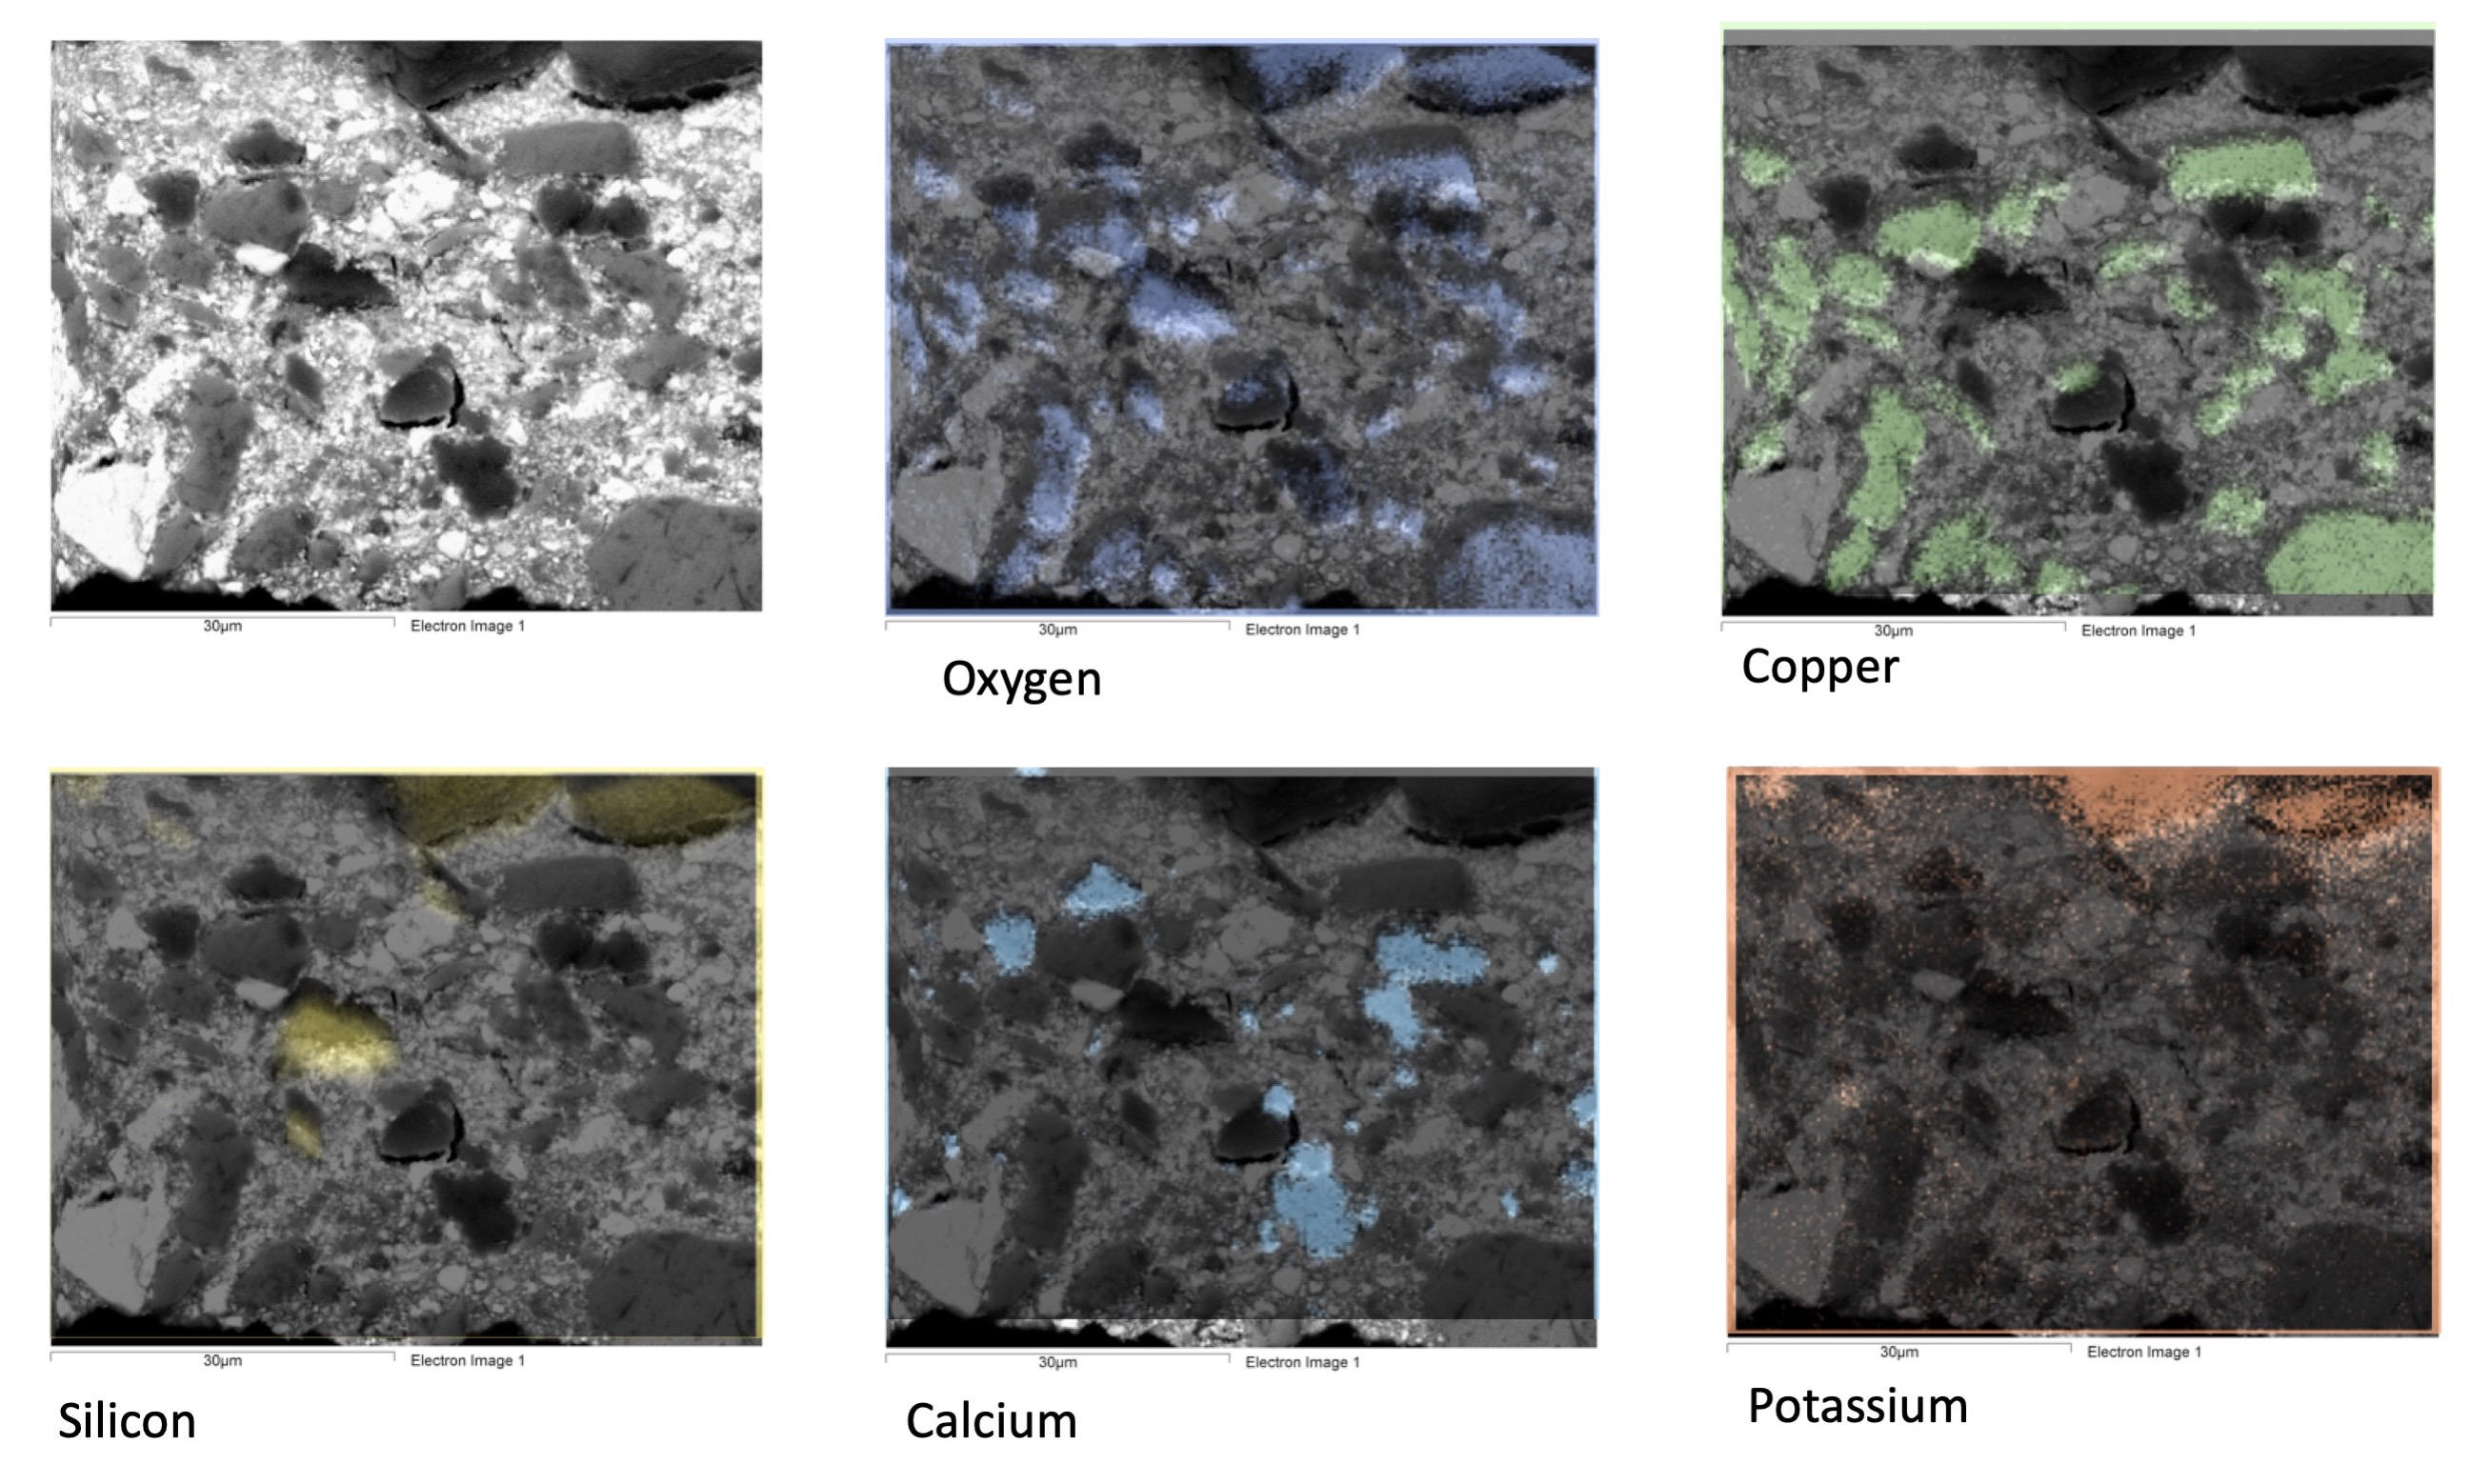
\includegraphics[width=0.9\linewidth]{1259.21_mapdata_1}
\hfill
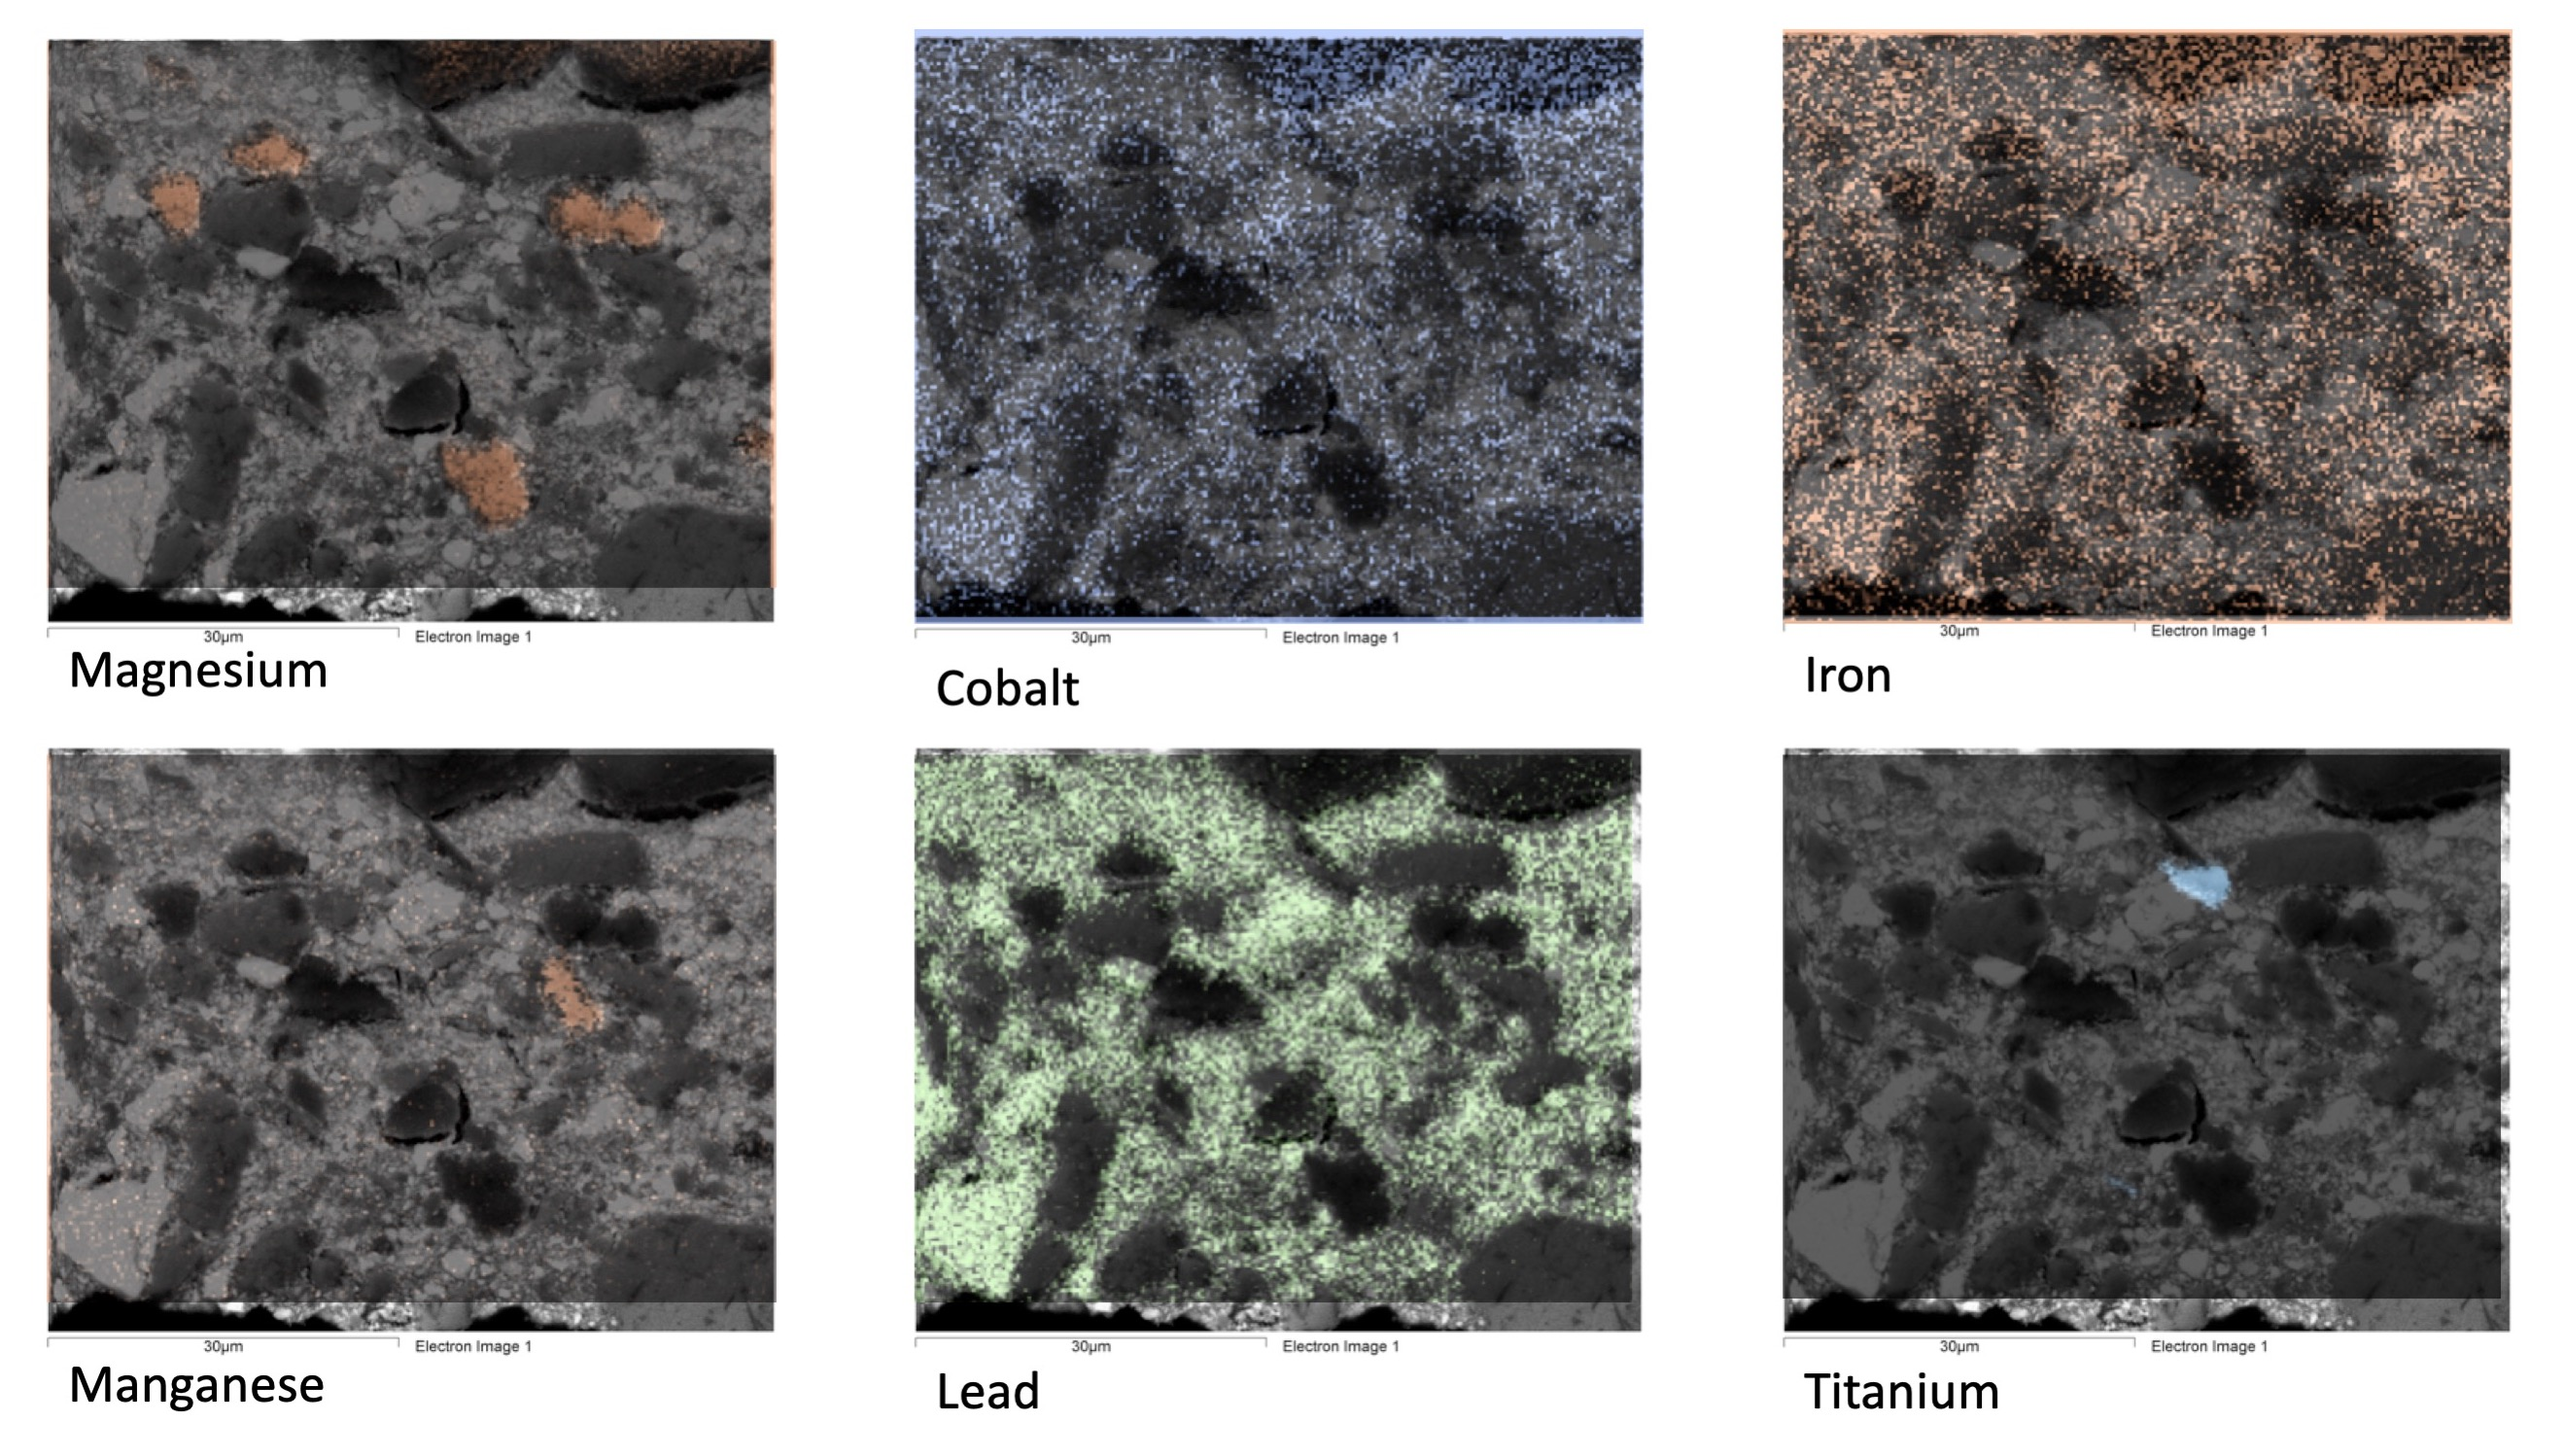
\includegraphics[width=0.9\linewidth]{1259.21_mapdata_2}
\hfill
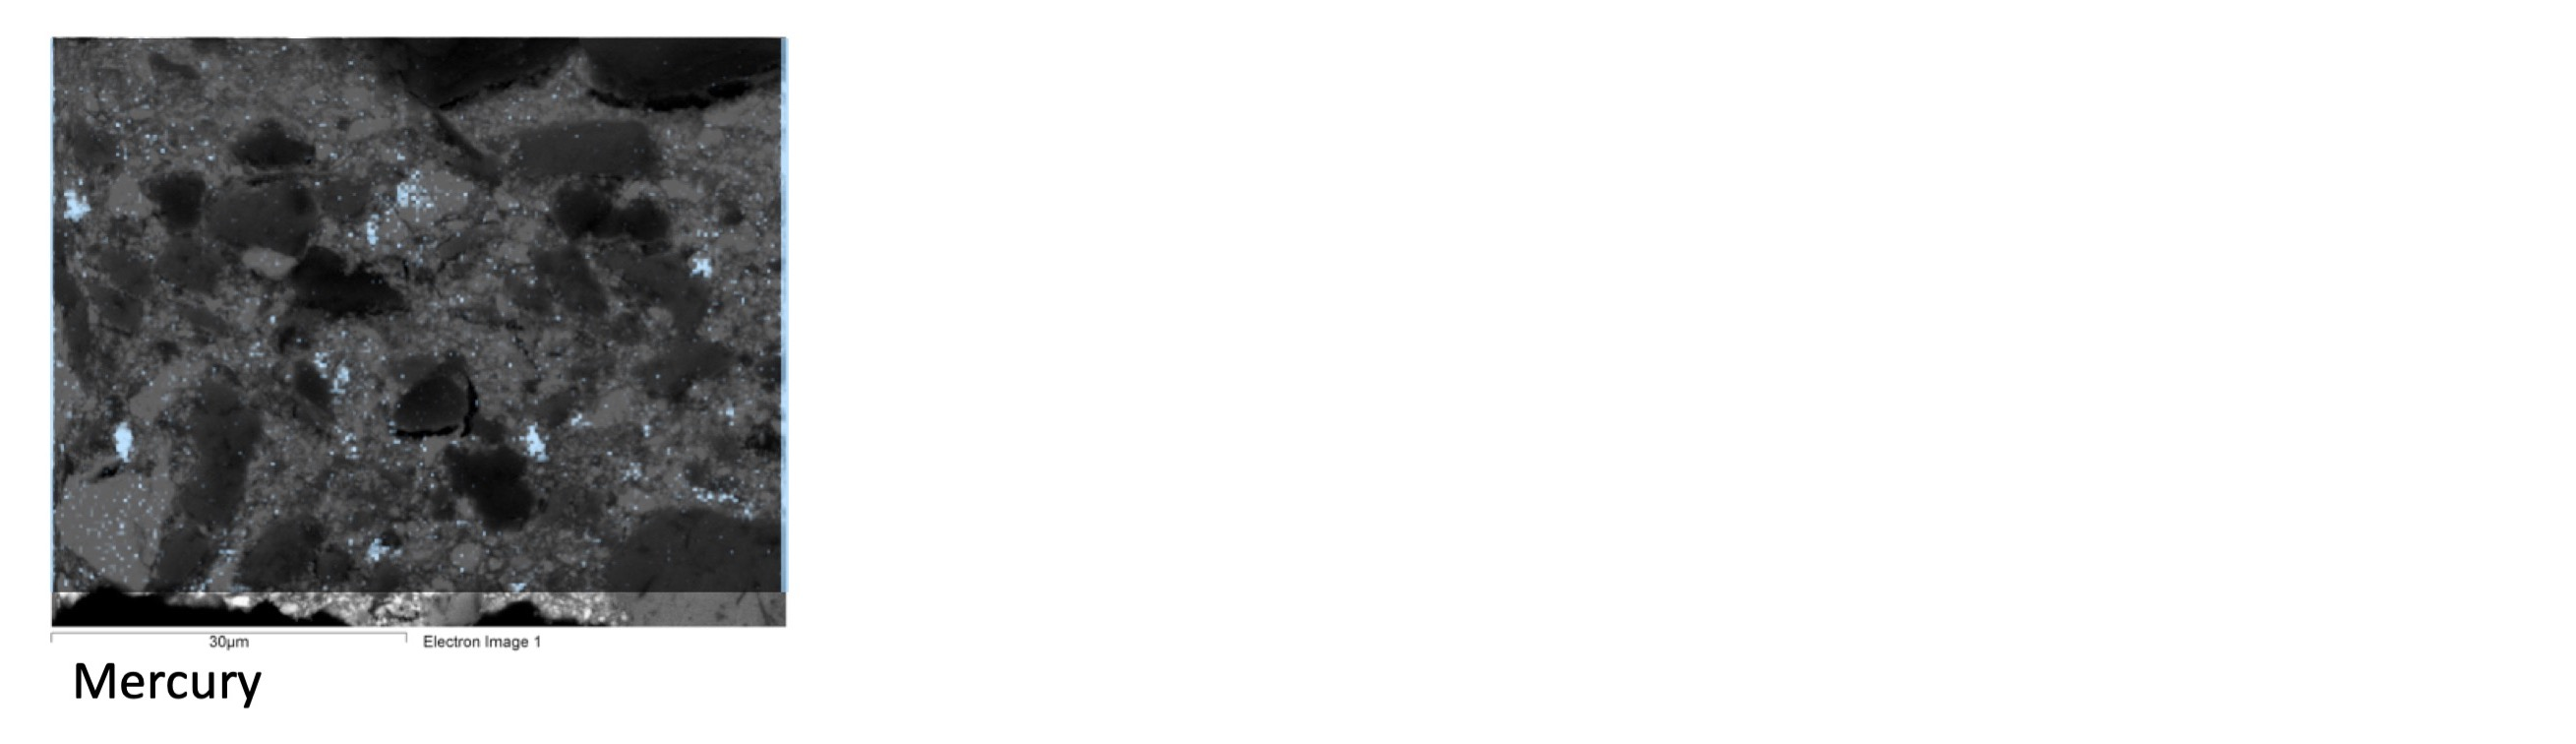
\includegraphics[width=0.9\linewidth]{1259.21_mapdata_3}
\hfill
\end{minipage}
\caption[EDS map data, sample 1259.21.]{EDS map data of sample 1259.21 showing locations of elements in an area of the azurite paint layer. Elements detected are O, Cu, Si, Ca, K, Mg, Co, Fe, Mn, Pb, Ti, and Hg.}
\label{fig:1259.21_mapdata}
\end{figure}


\begin{figure}[H]
\centering
  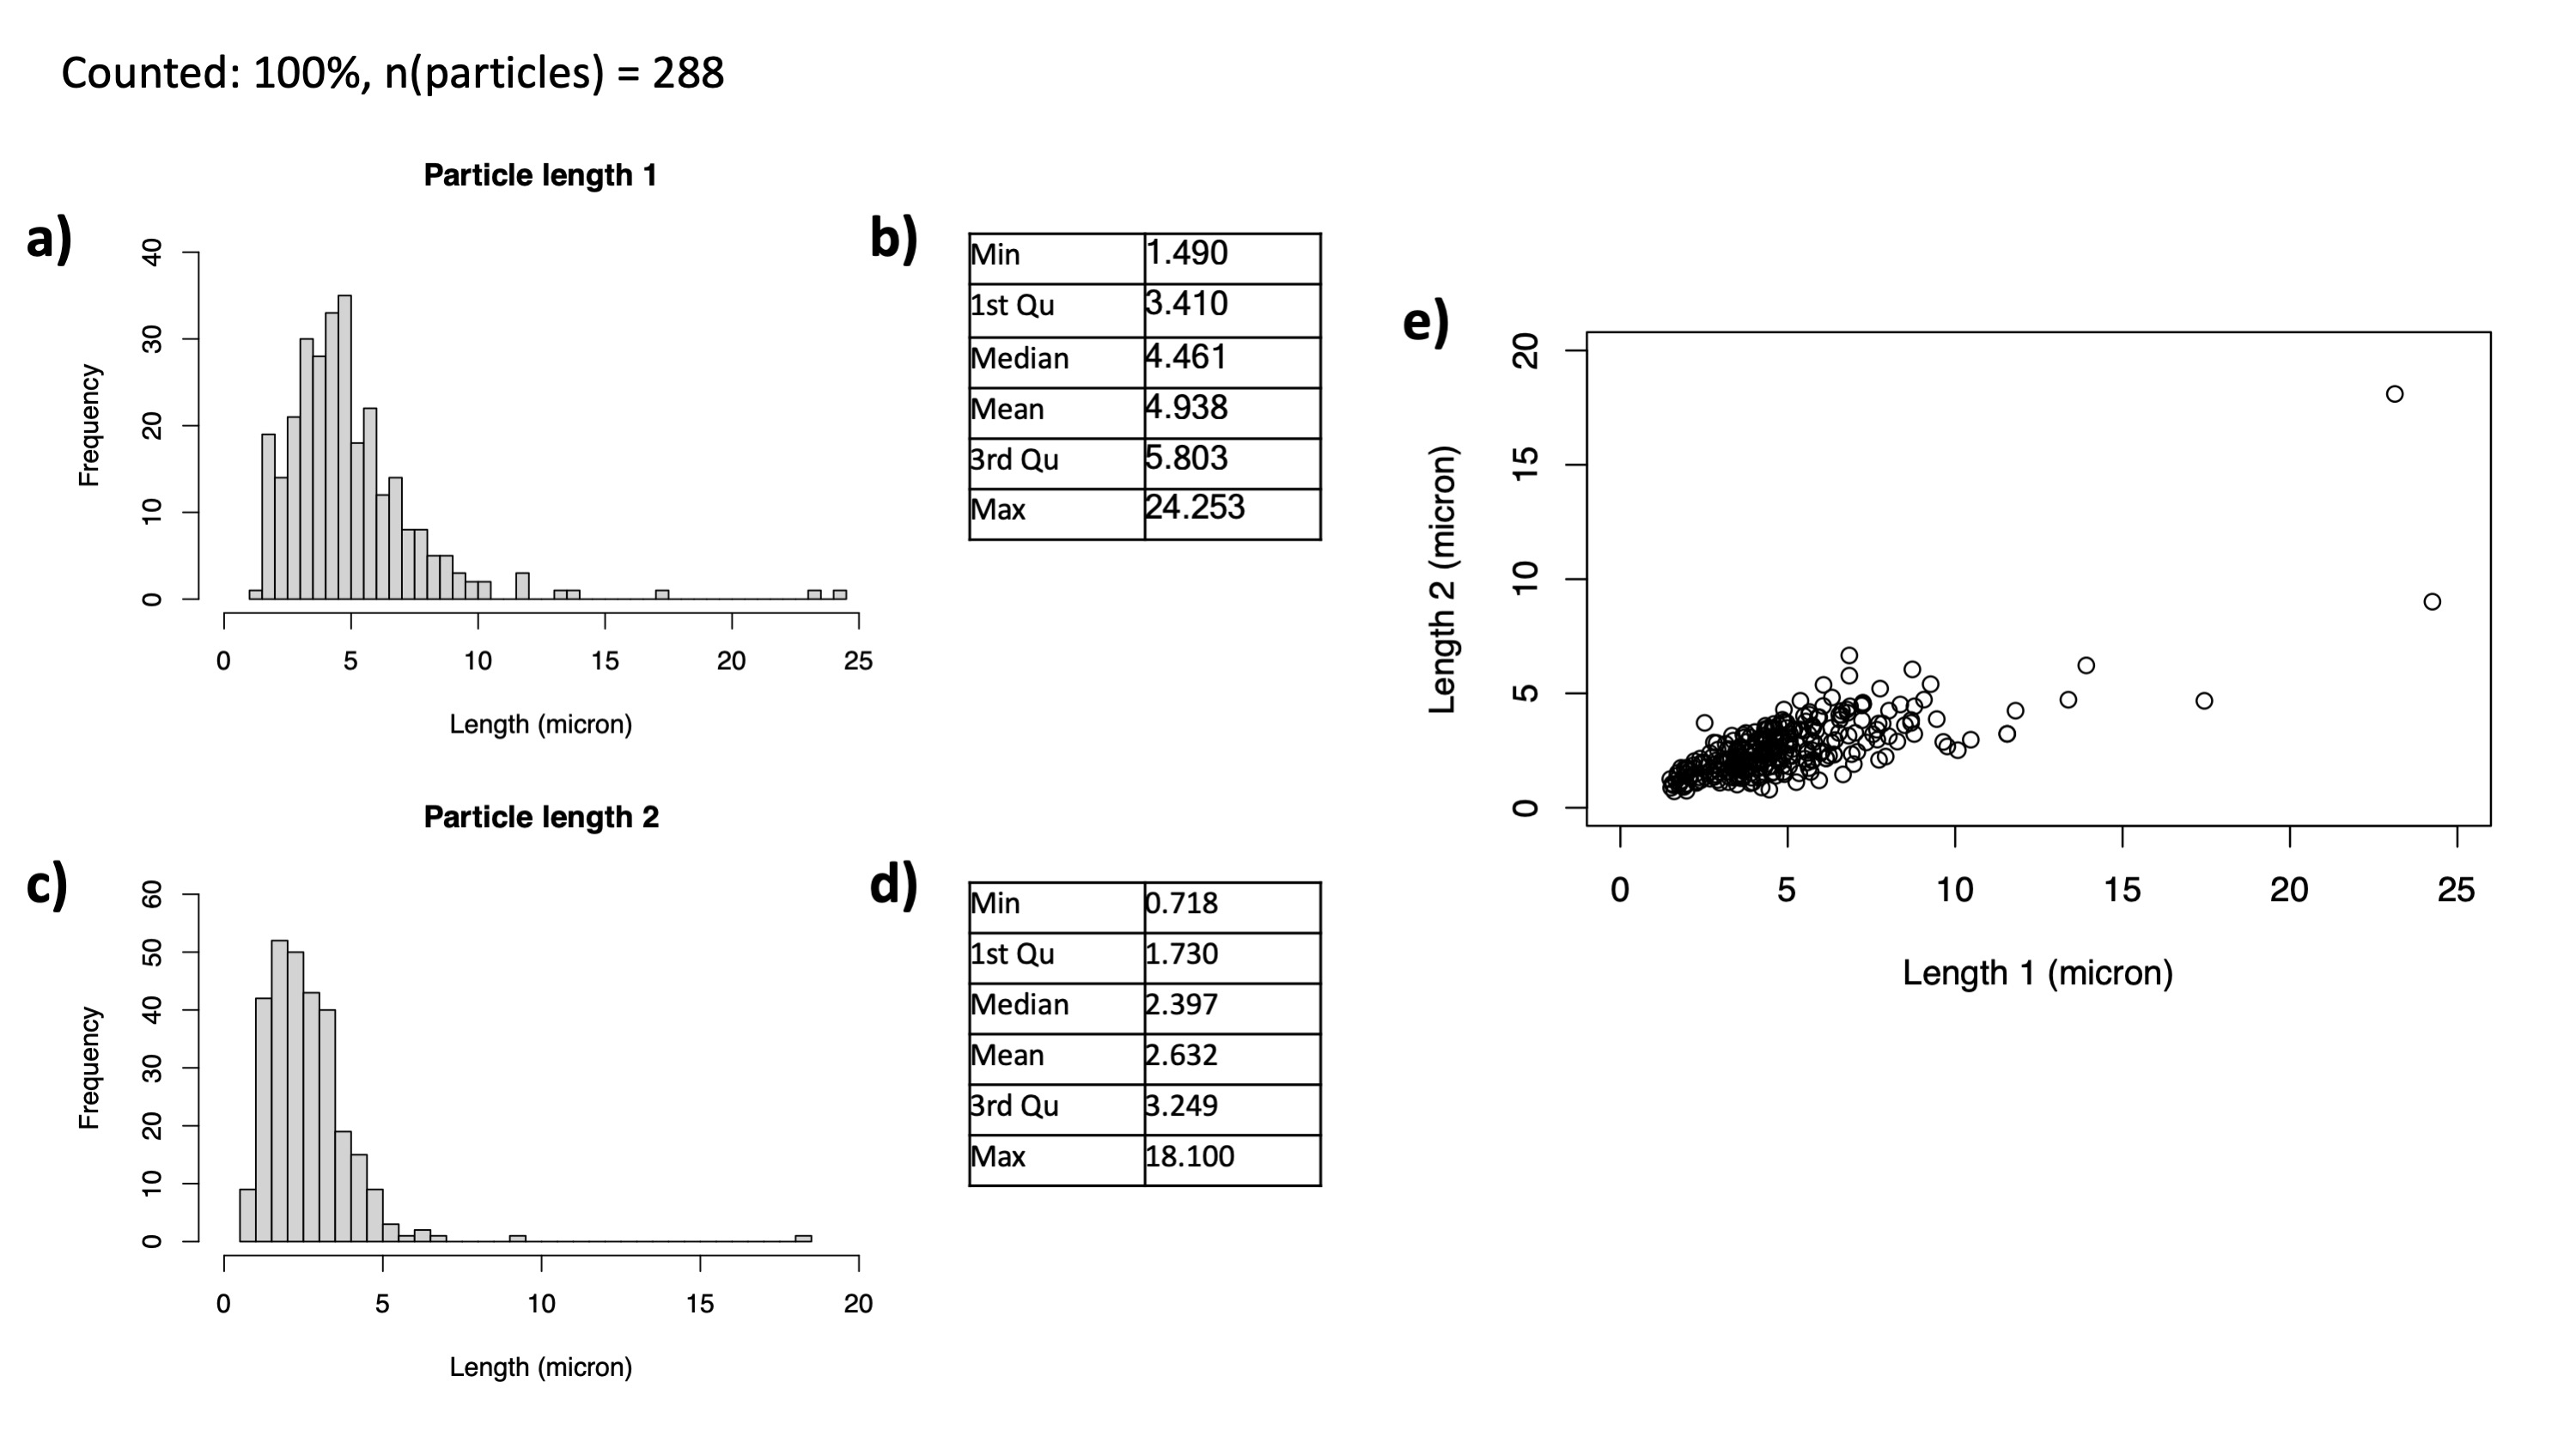
\includegraphics[width=0.8\linewidth]{1259.21_partsize}
\caption[Particle size distribution, sample 1259.21.]{Particle size distribution of sample 1259.21: \textbf{a)} Histogram showing distribution of particle length 1 values. \textbf{b)} Descriptive statistics for particle length 1 data. \textbf{c)} Histogram showing distribution of particle length 2 values. \textbf{d)} Descriptive statistics for particle length 2 data. \textbf{e)} Graph of length 1 versus length 2 showing the degree of skew.}
\label{fig:1259.21_partsize}
\end{figure}


\section{Sample 1259.23}


\begin{figure}[H]
  \centering
  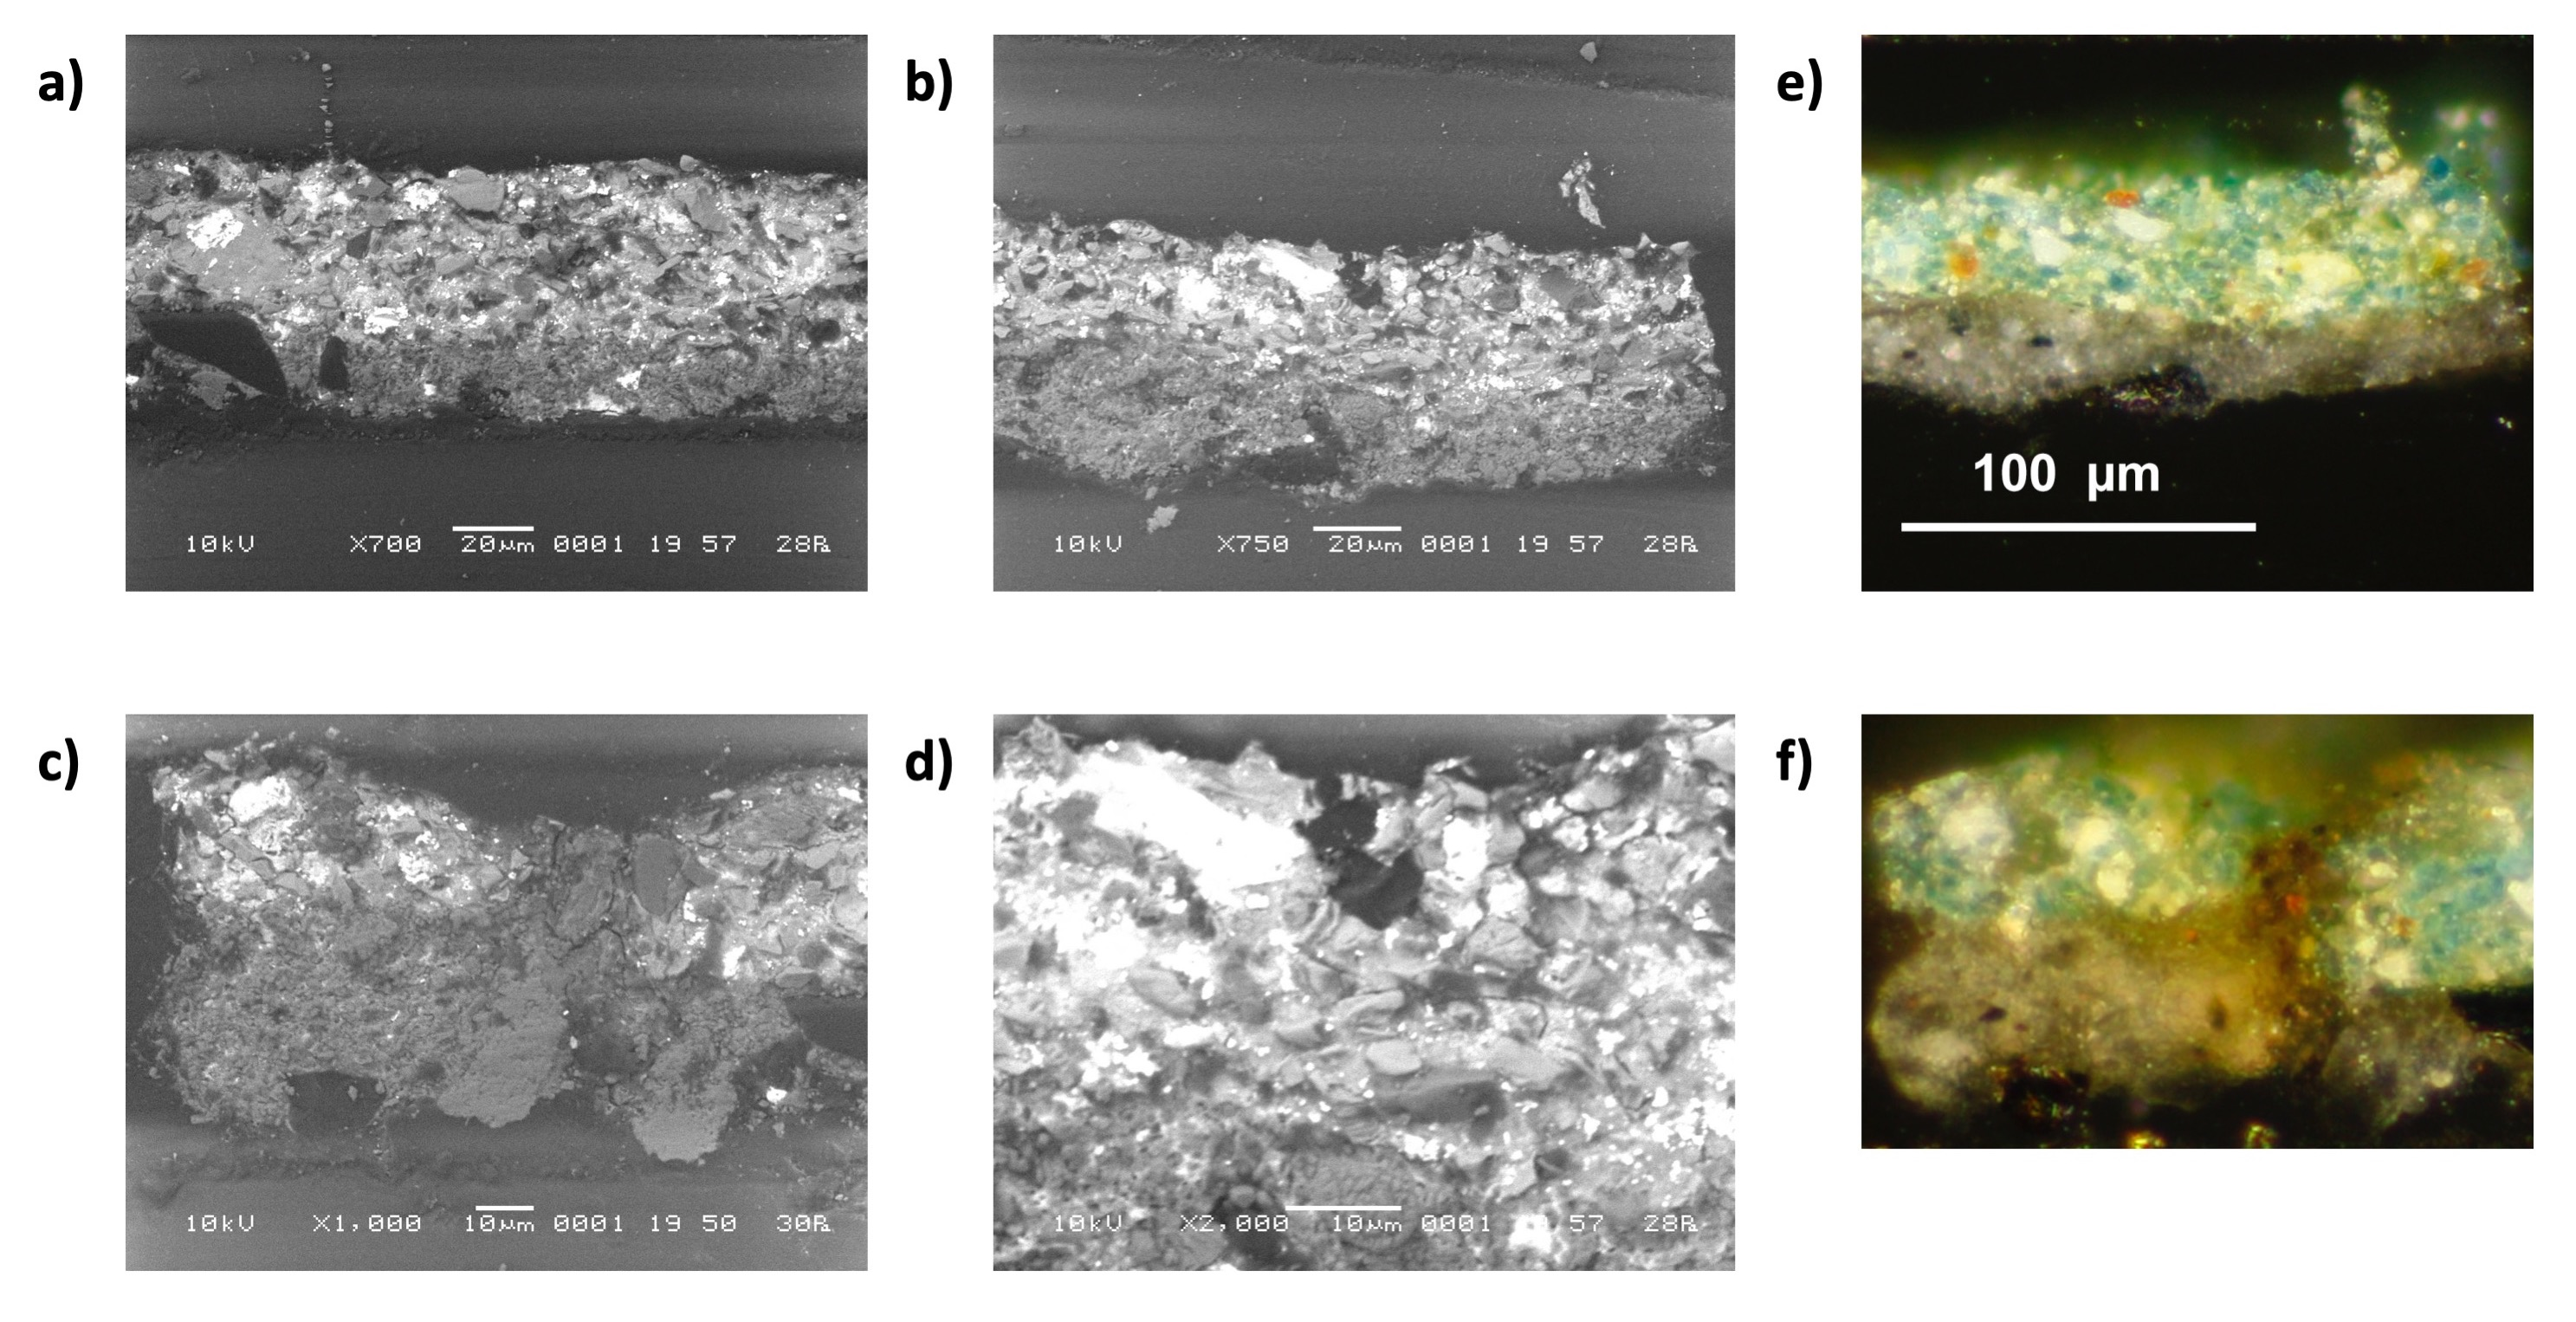
\includegraphics[width=0.8\linewidth]{1259.23_imgs}
\caption[SEM and dark field images of sample 1259.21.]{SEM and dark field images of sample 1259.21: \textbf{a)} 700x magnification, \textbf{b)} 750x magnification, \textbf{c)} 1000x magnification, \textbf{d)} 2000x magnification, \textbf{e)} and \textbf{f)}, dark field microscope images corresponding to \textbf{b} and \textbf{c} respectively. Dark field microscope images courtesy of Katharine Waldron, HKI.}
\label{fig:1259.23_imgs}
\end{figure}

\begin{figure}[H]
  \centering
  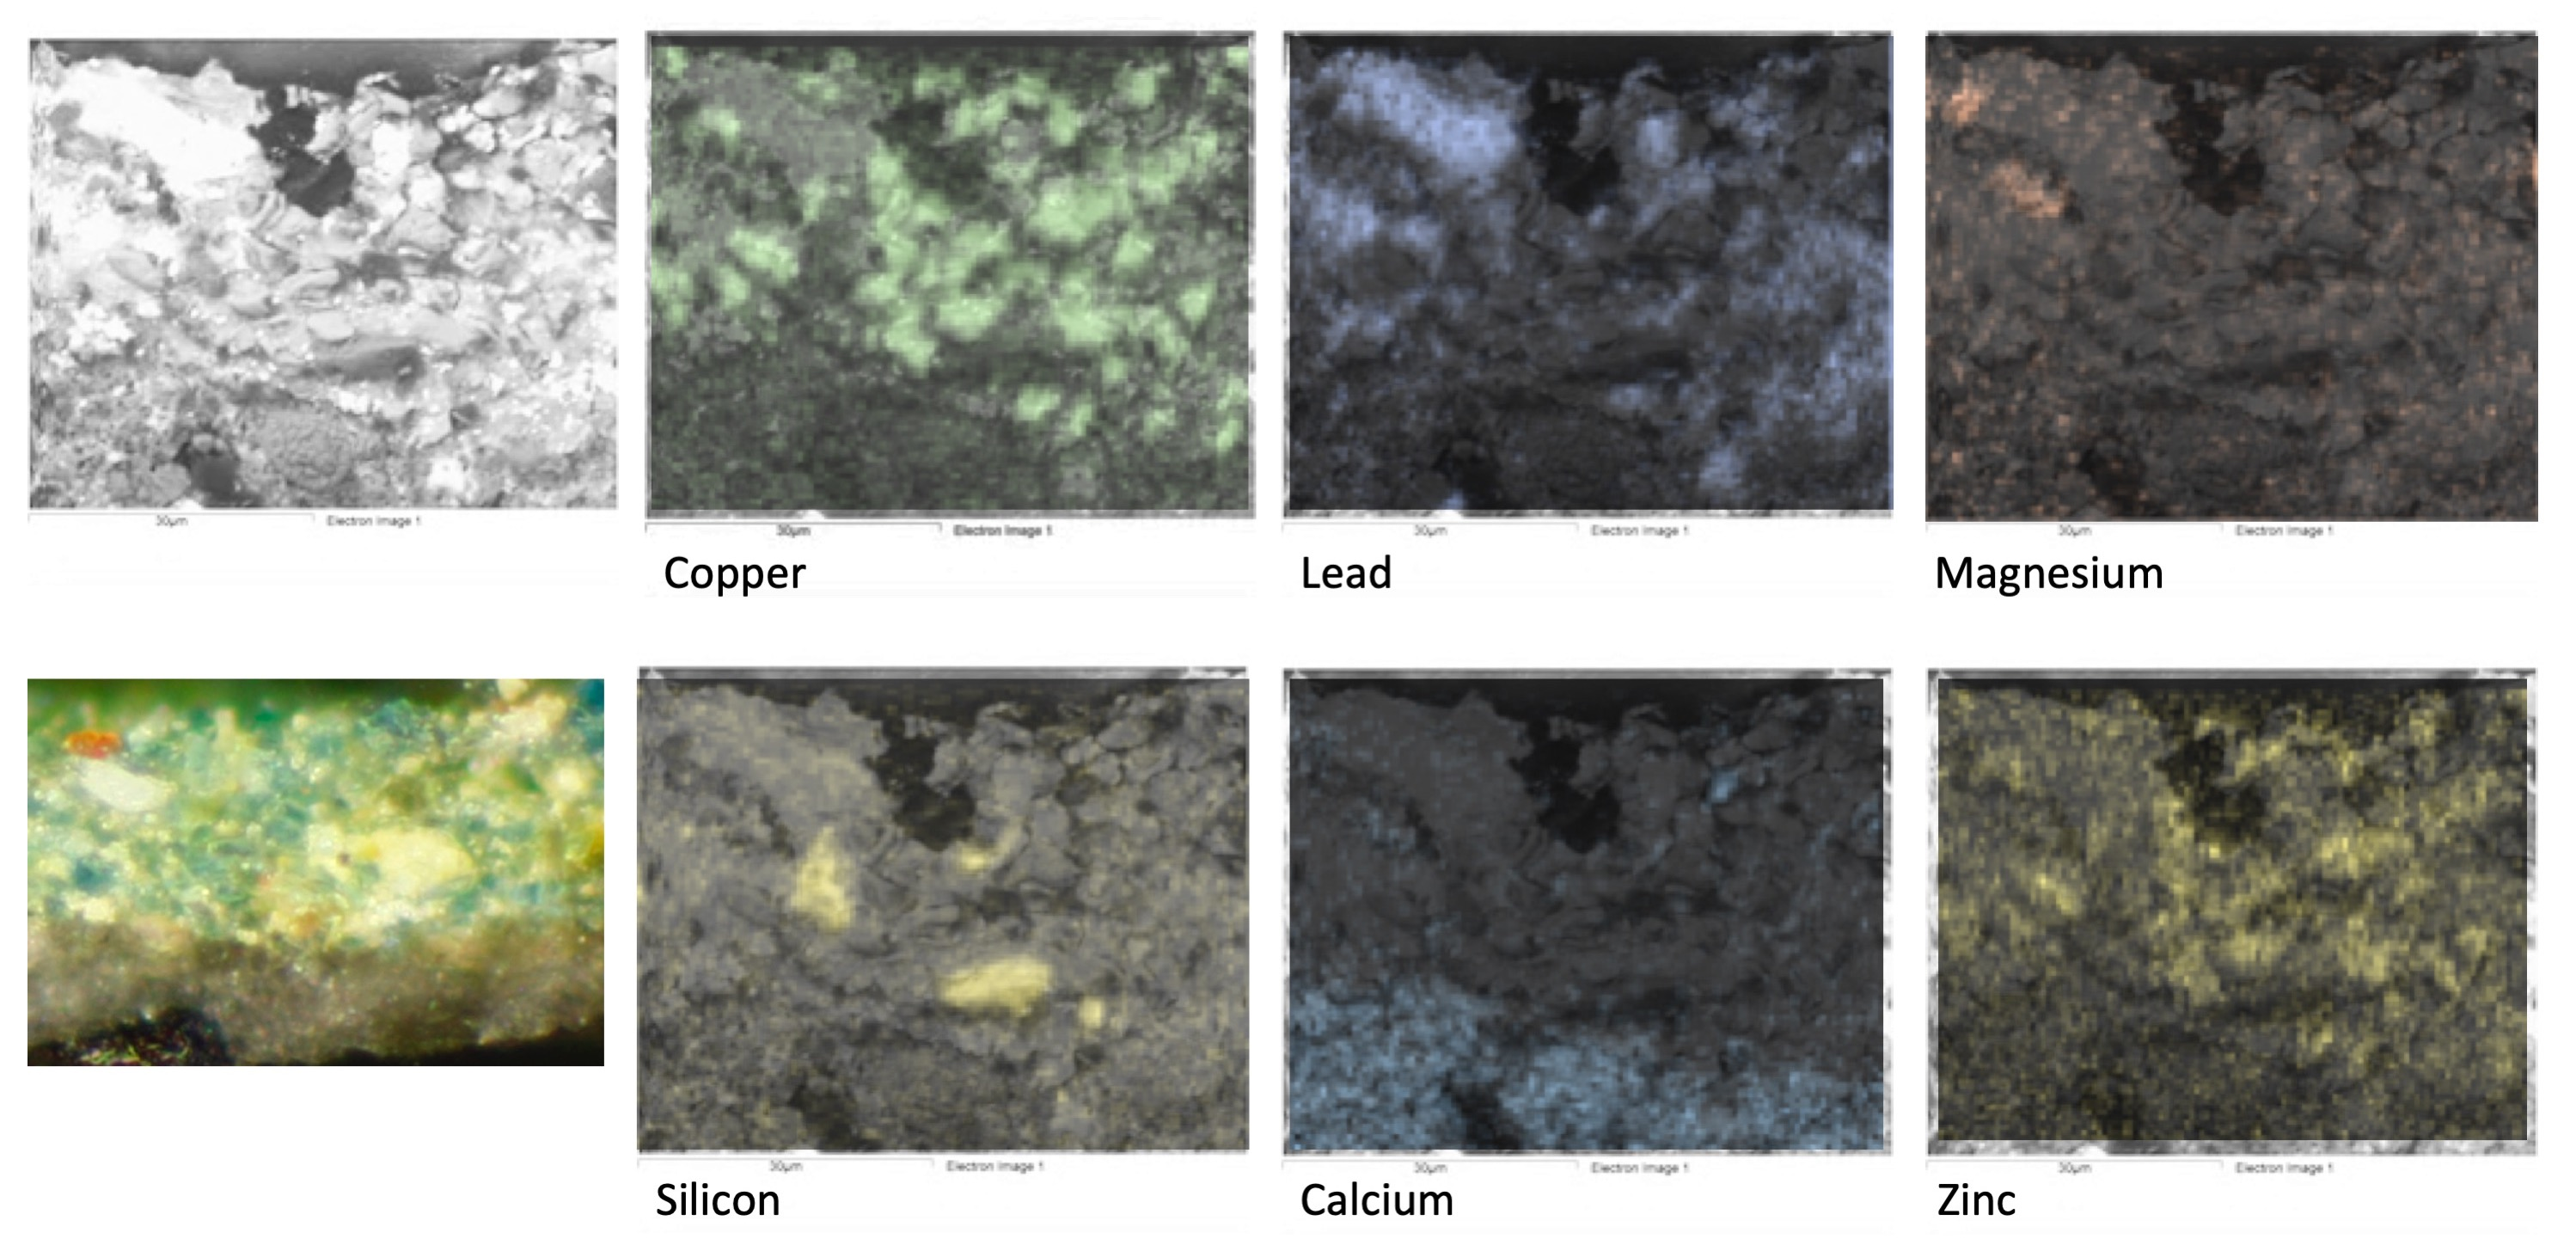
\includegraphics[width=0.8\linewidth]{1259.23_mapdata}
\caption[EDS map data, sample 1259.23.]{EDS map data of sample 1259.23 showing locations of elements in an area of the azurite paint layer. Elements detected are Cu, Pb, Mg, Si, Ca, Zn. SEM and dark field microscope images of mapped area are also shown. The dark field microscope image is provided by Katharine Waldron, HKI.}
\label{fig:1259.23_mapdata}
\end{figure}


\begin{figure}[H]
\centering
  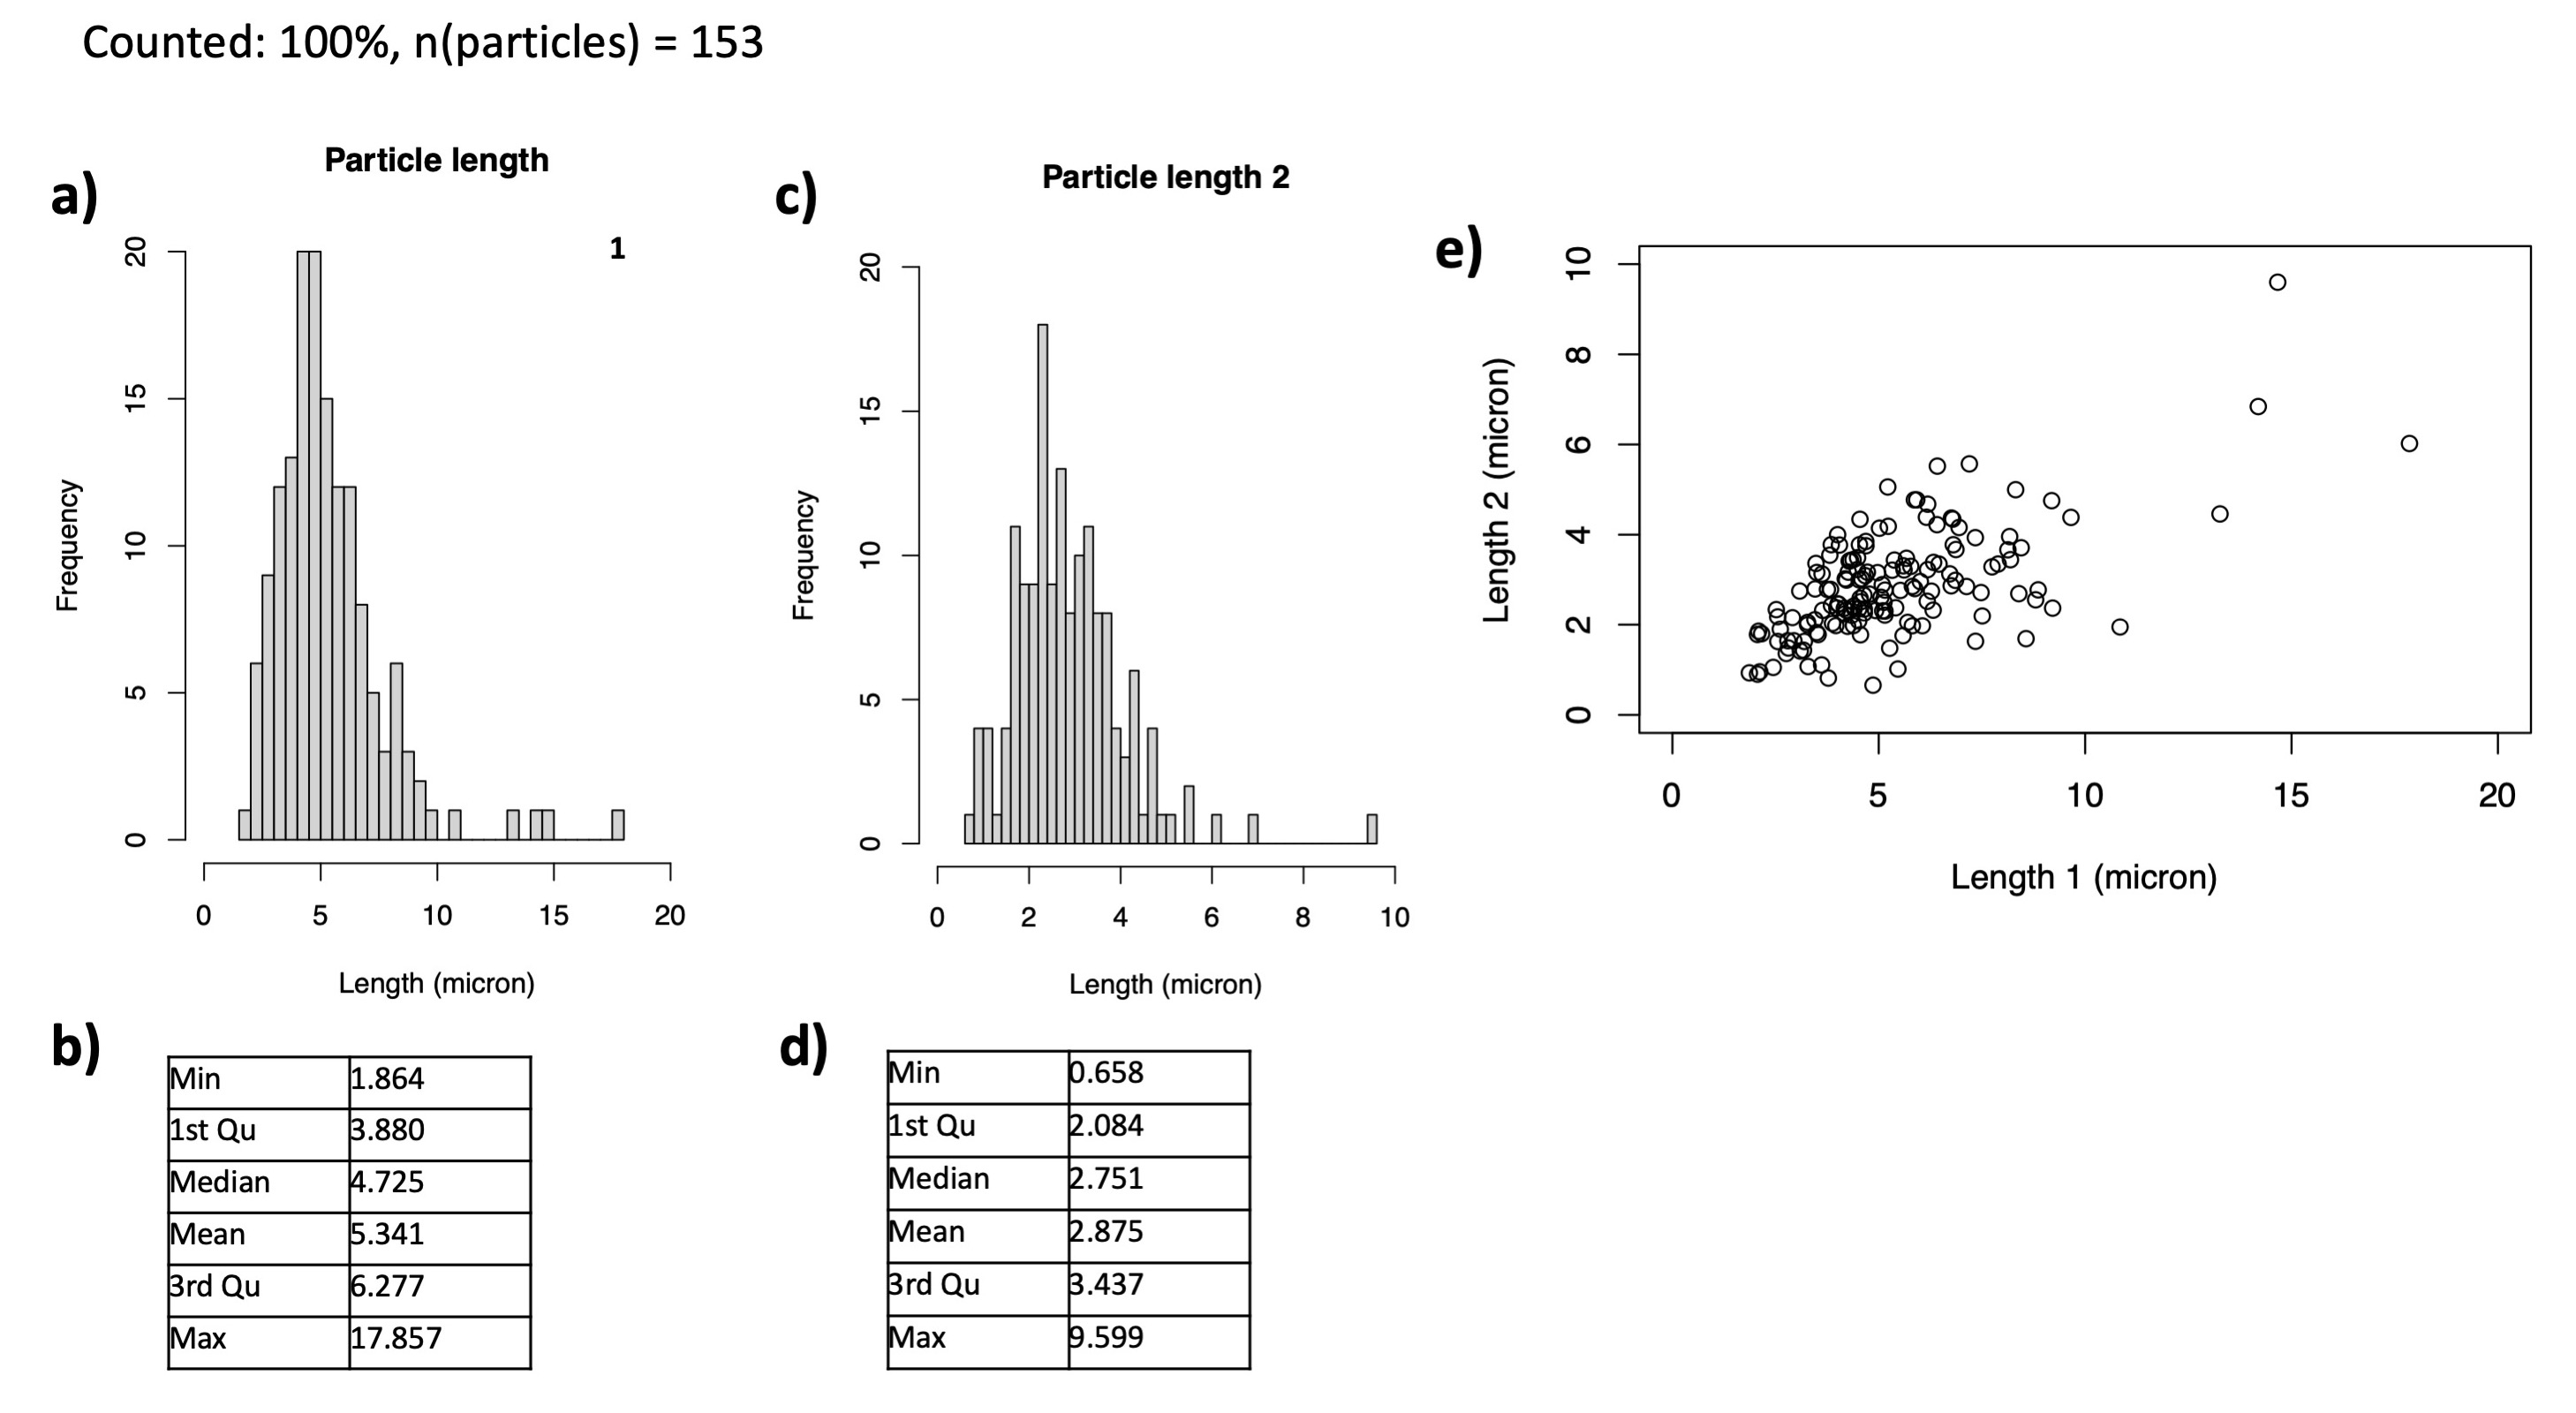
\includegraphics[width=0.8\linewidth]{1259.23_partsize}
\caption[Particle size distribution, sample 1259.23.]{Particle size distribution of sample 1259.23: \textbf{a)} Histogram showing distribution of particle length 1 values. \textbf{b)} Descriptive statistics for particle length 1 data. \textbf{c)} Histogram showing distribution of particle length 2 values. \textbf{d)} Descriptive statistics for particle length 2 data. \textbf{e)} Graph of length 1 versus length 2 showing the degree of skew.}
\label{fig:1259.23_partsize}
\end{figure}



\section{Sample 1259.28}


\begin{figure}[H]
  \centering
  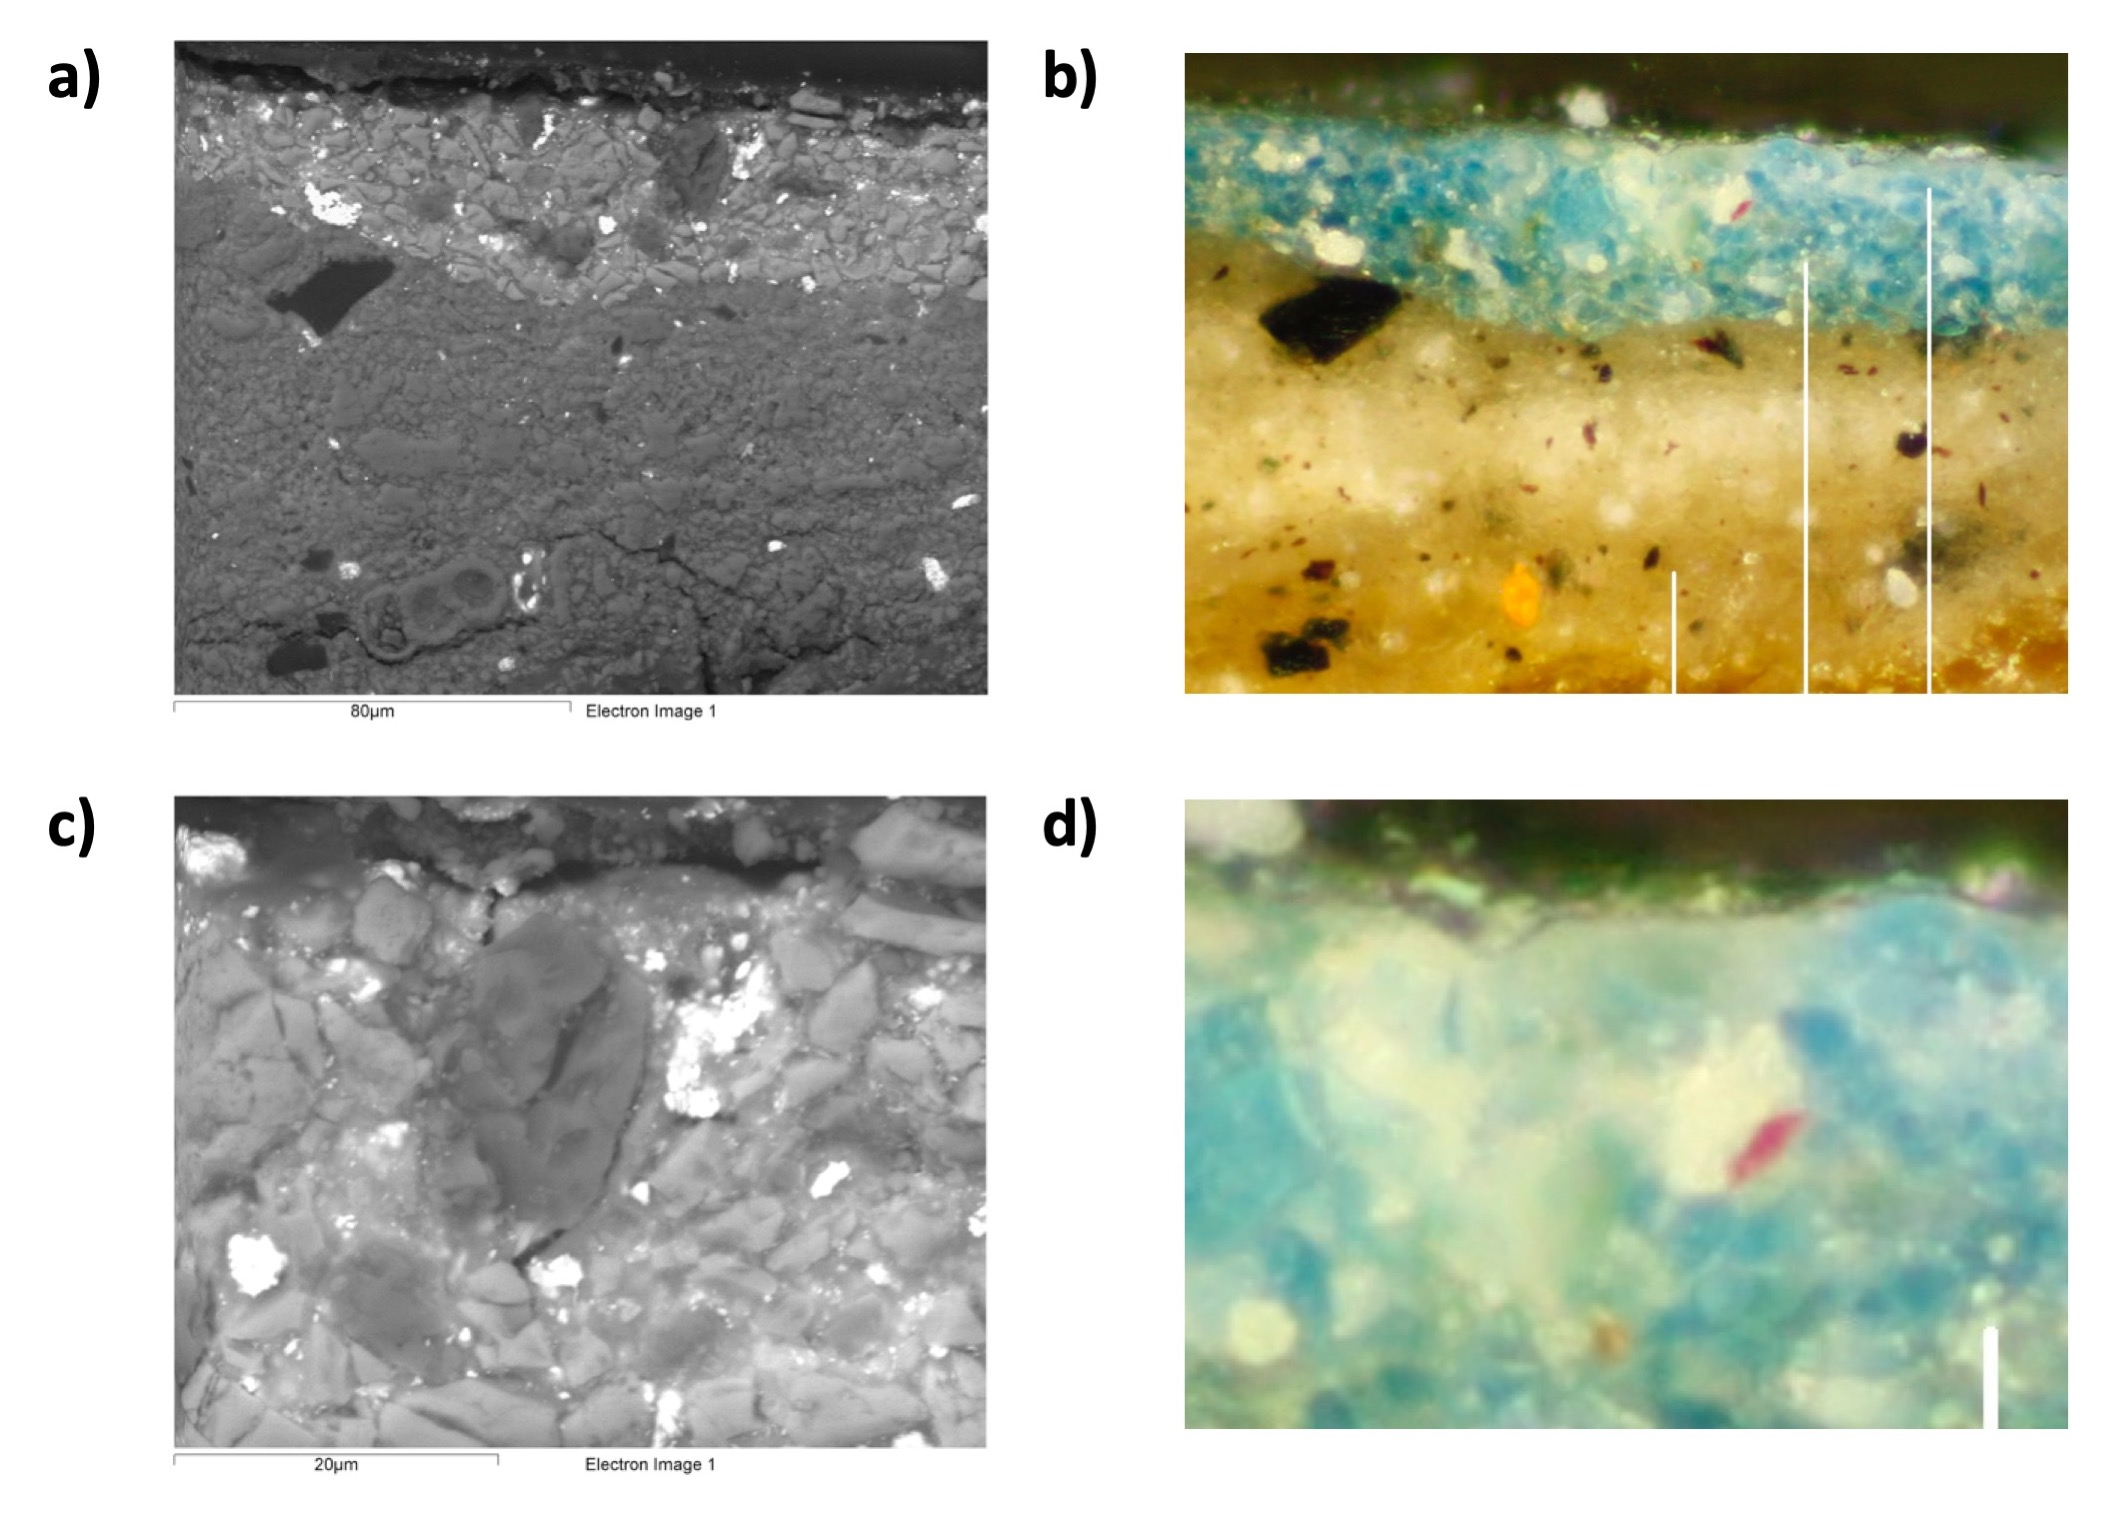
\includegraphics[width=0.8\linewidth]{1259.28_imgs}
\caption[SEM and dark field images of sample 1259.28.]{SEM and dark field images of sample 1259.28: \textbf{a)} 750x magnification, \textbf{b)} corresponding dark field microscope image, \textbf{c)} 2000x magnification, \textbf{d)} corresponding dark field microscope image. Dark field microscope images courtesy of Katharine Waldron, HKI.}
\label{fig:1259.28_imgs}
\end{figure}

\begin{figure}[H]
  \centering
  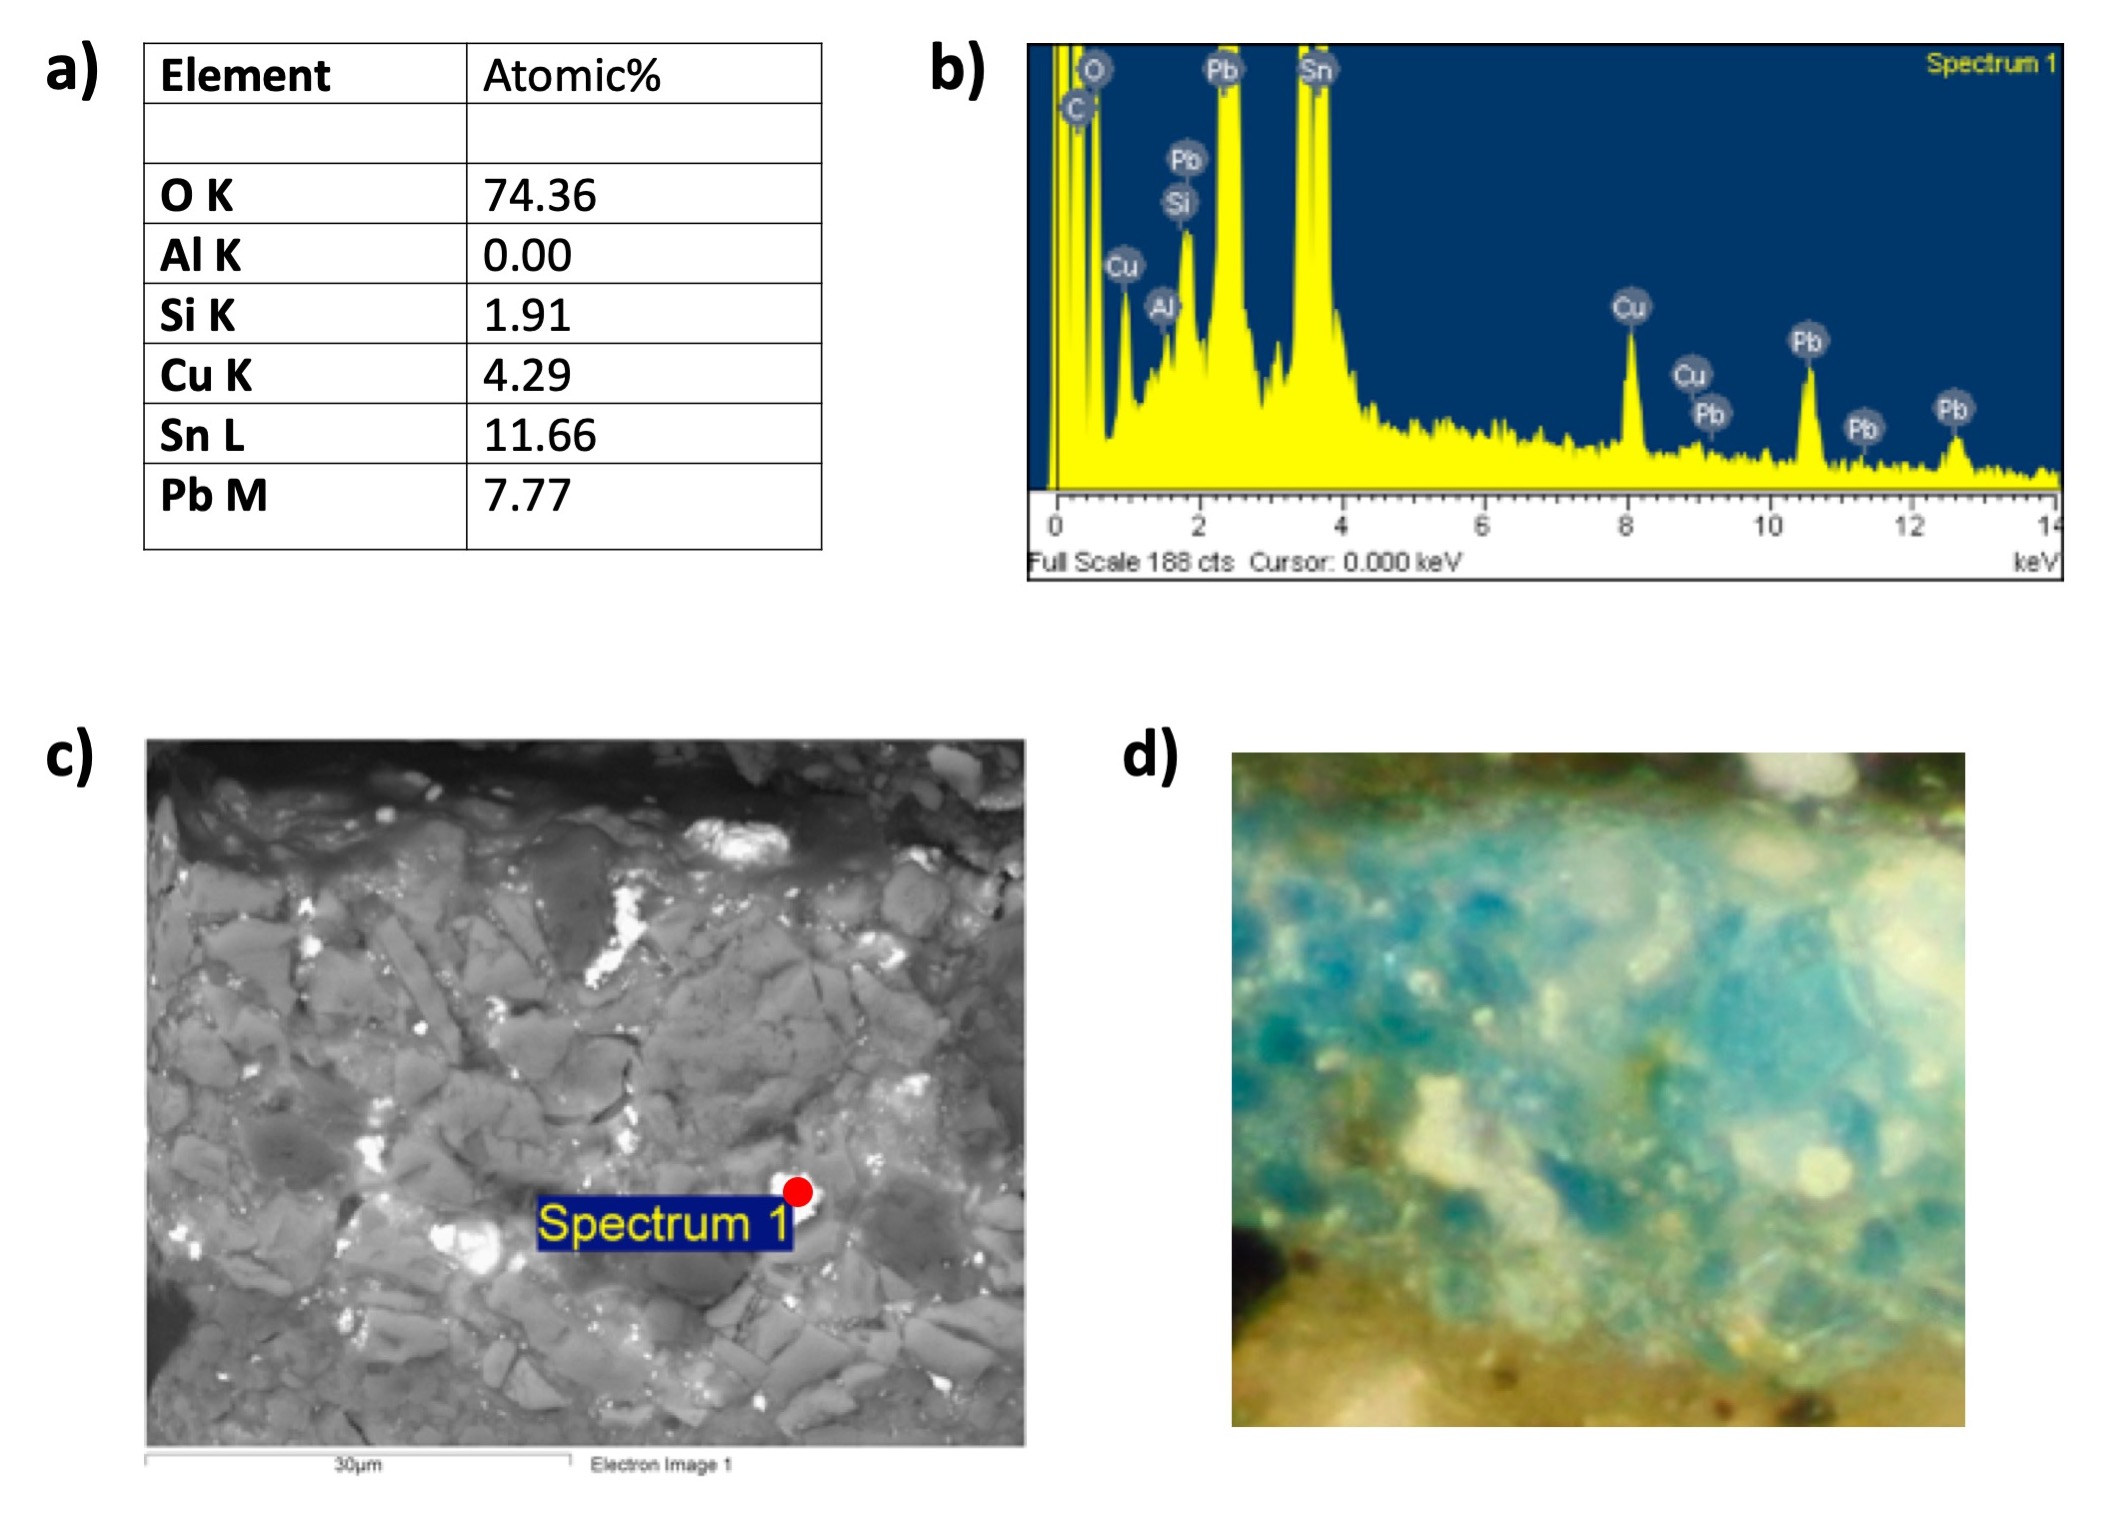
\includegraphics[width=0.8\linewidth]{1259.28_pointspec}
\caption[EDS point spectrum data, sample 1259.28.]{EDS point spectrum data, sample 1259.28: \textbf{a)} Quantitative EDS results of particle showing lead and tin, \textbf{b)} EDS spectrum showing detection of lead and tin, \textbf{c)} SEM image showing point spectrum location, \textbf{d)} dark field microscope image showing point spectrum sample location, with no visually distinct particle present. Image is provided courtesy of Katharine Waldron, HKI.}
\label{fig:1259.28_pointspec}
\end{figure}

\begin{figure}[H]
\centering
\begin{minipage}[t]{\linewidth}
  \centering
  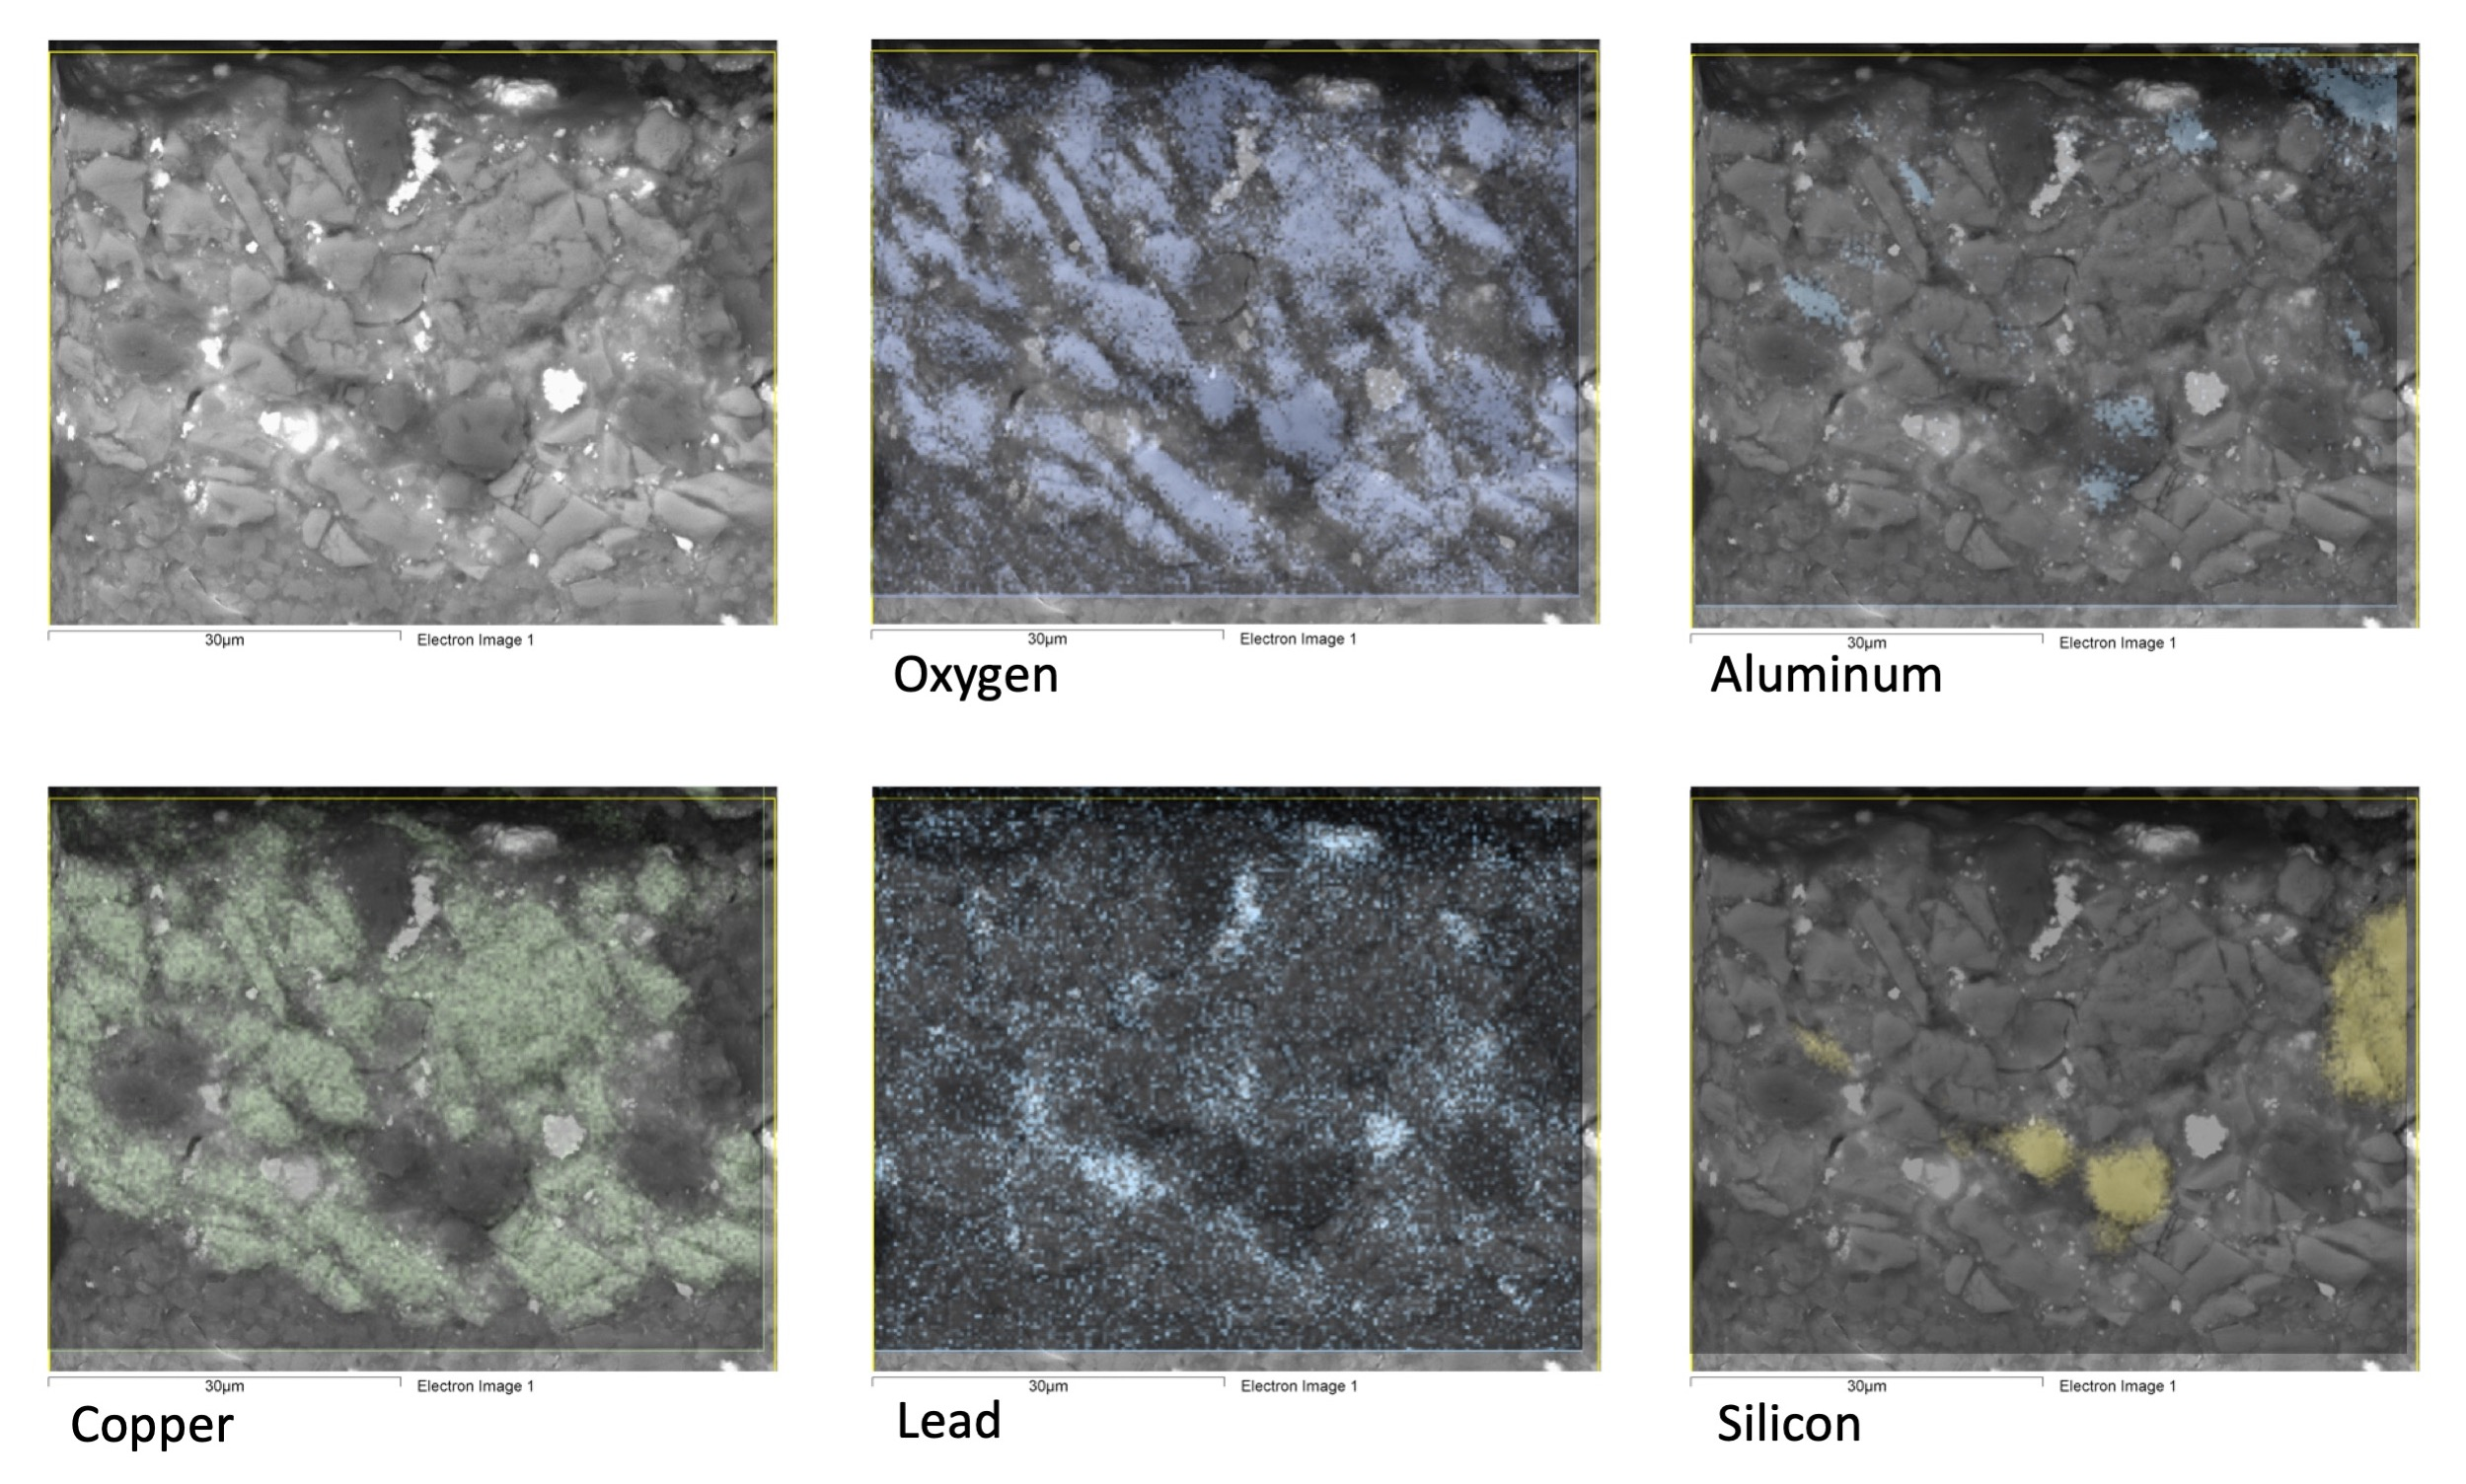
\includegraphics[width=0.9\linewidth]{1259.28_mapdata_1}
\hfill
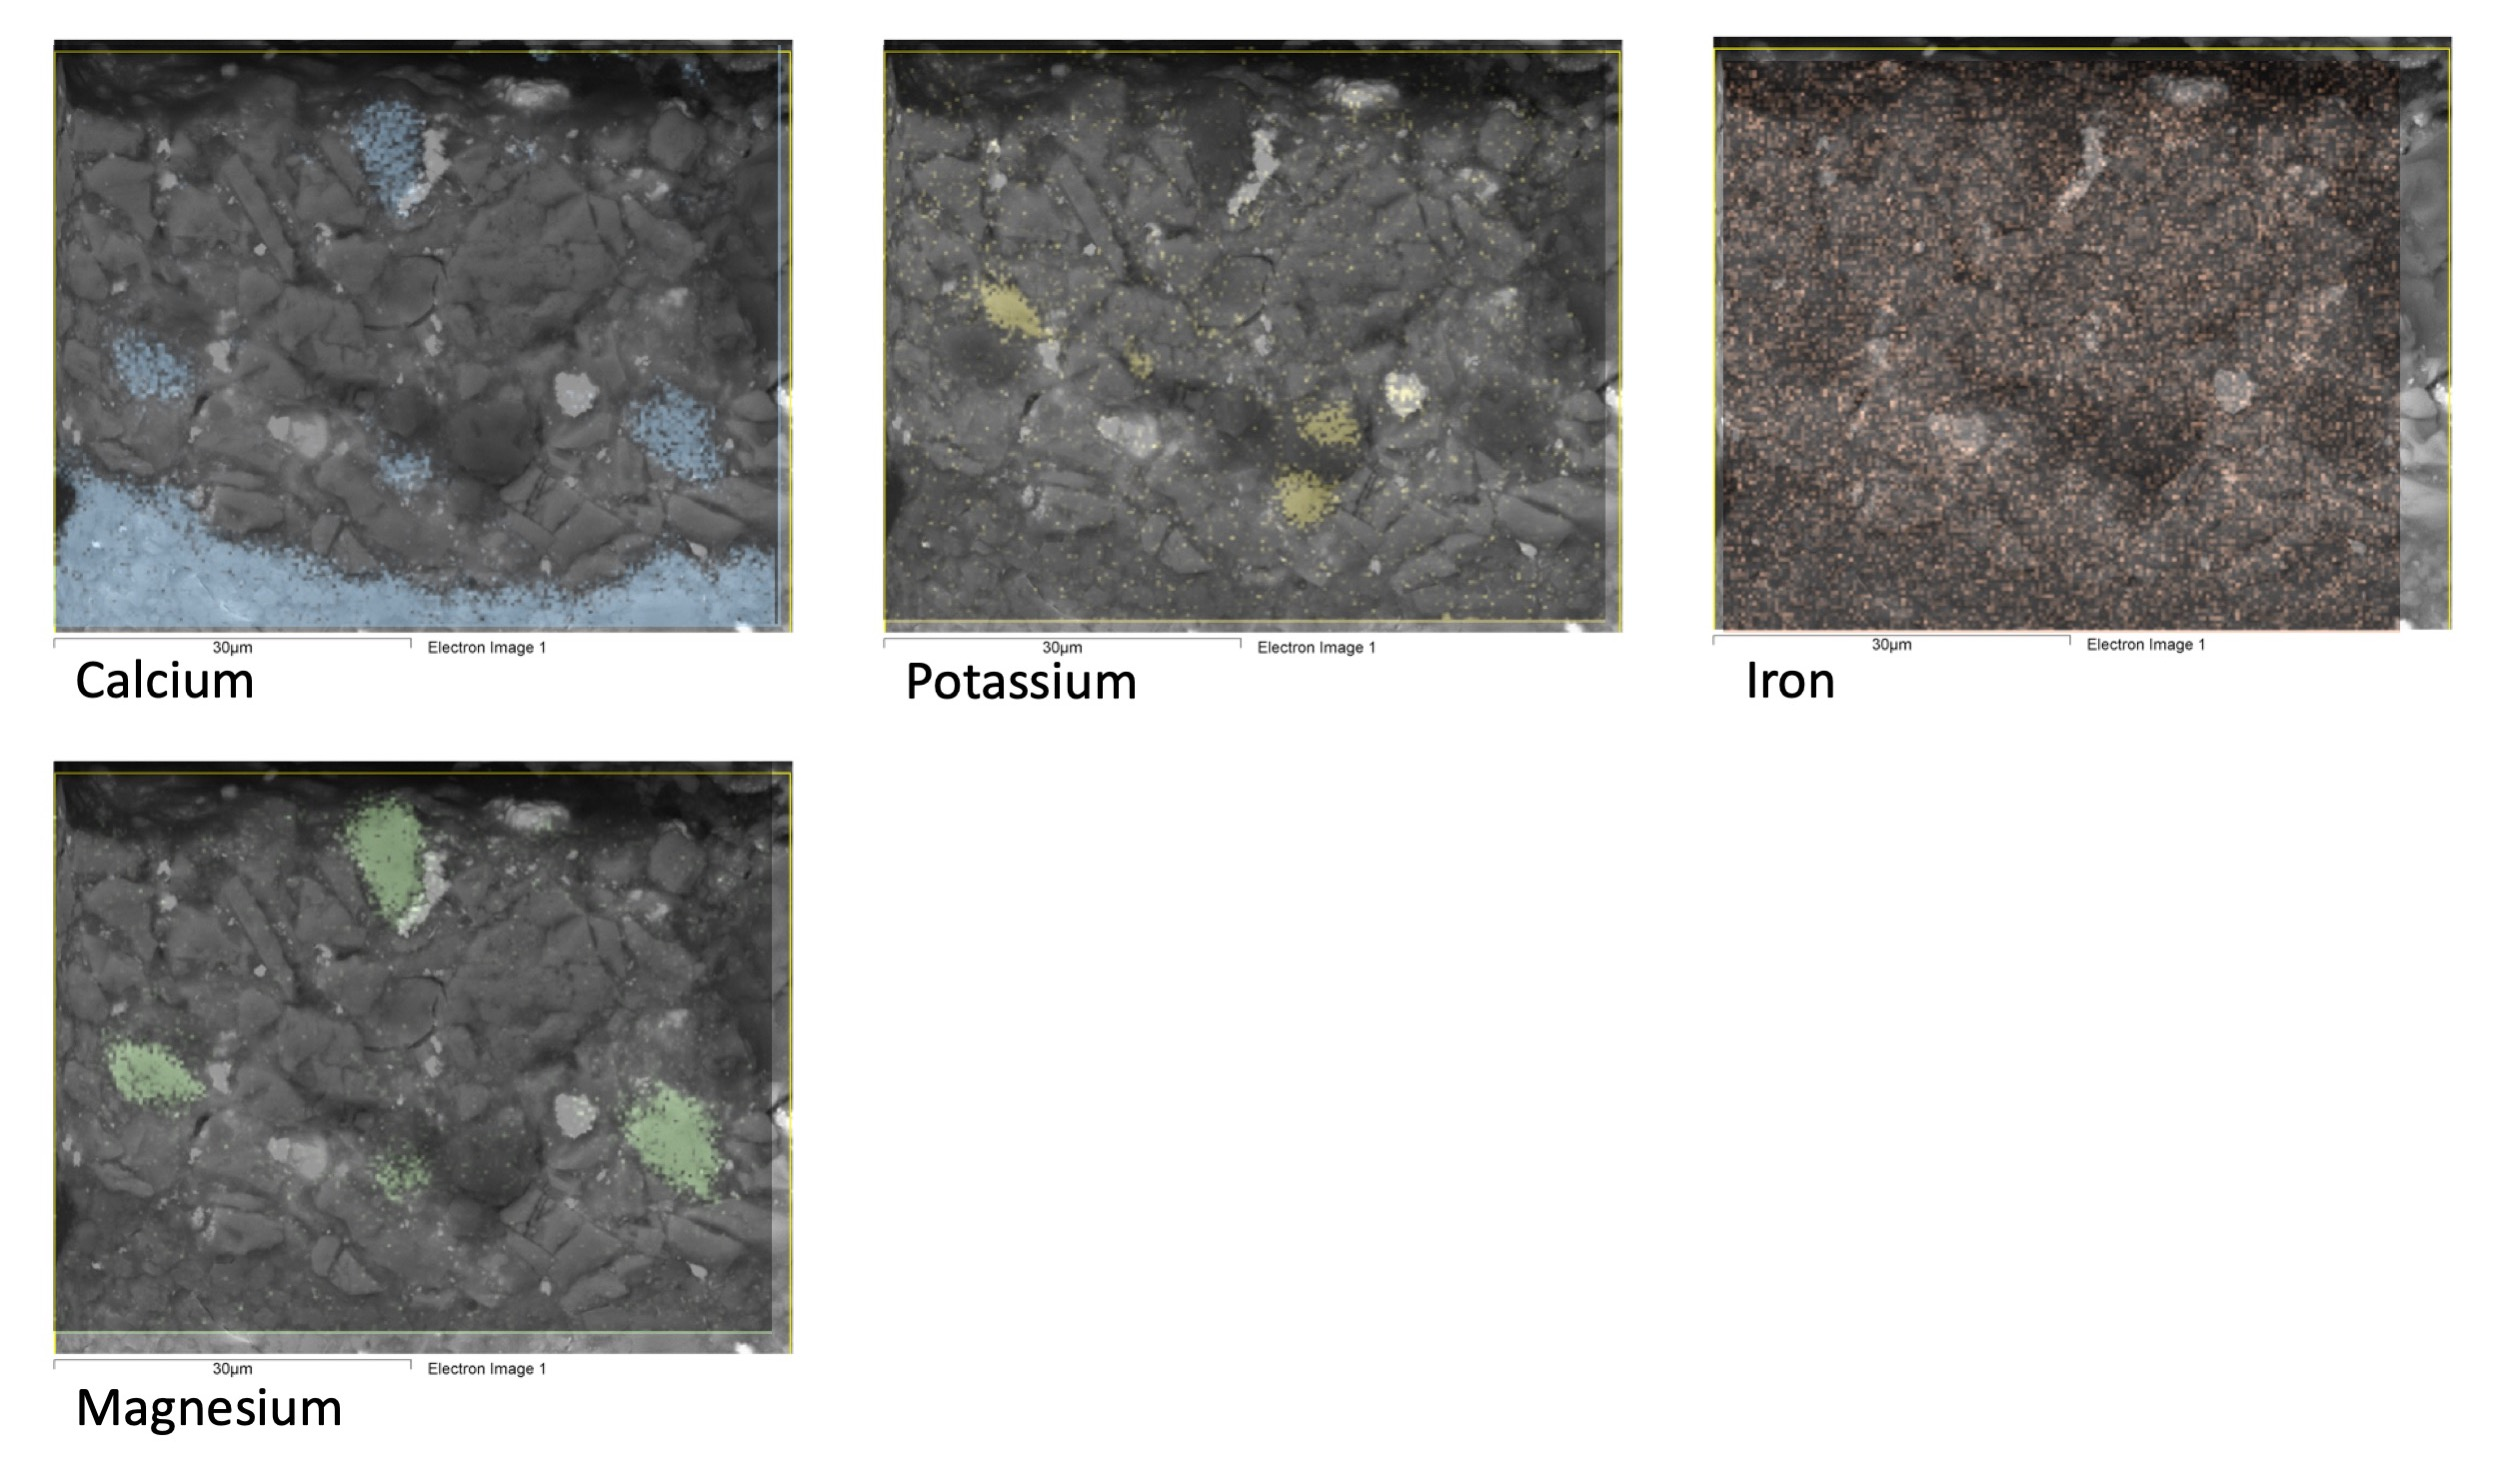
\includegraphics[width=0.9\linewidth]{1259.28_mapdata_2}
\hfill
\end{minipage}
\caption[EDS map data, sample 1259.28.]{EDS map data of sample 1259.28 showing locations of elements in an area of the azurite paint layer. Elements detected are O, Al, Cu, Pb, Si, Ca, K, Fe, Mg.}
\label{fig:1259.28_mapdata}
\end{figure}

\begin{figure}[H]
\centering
  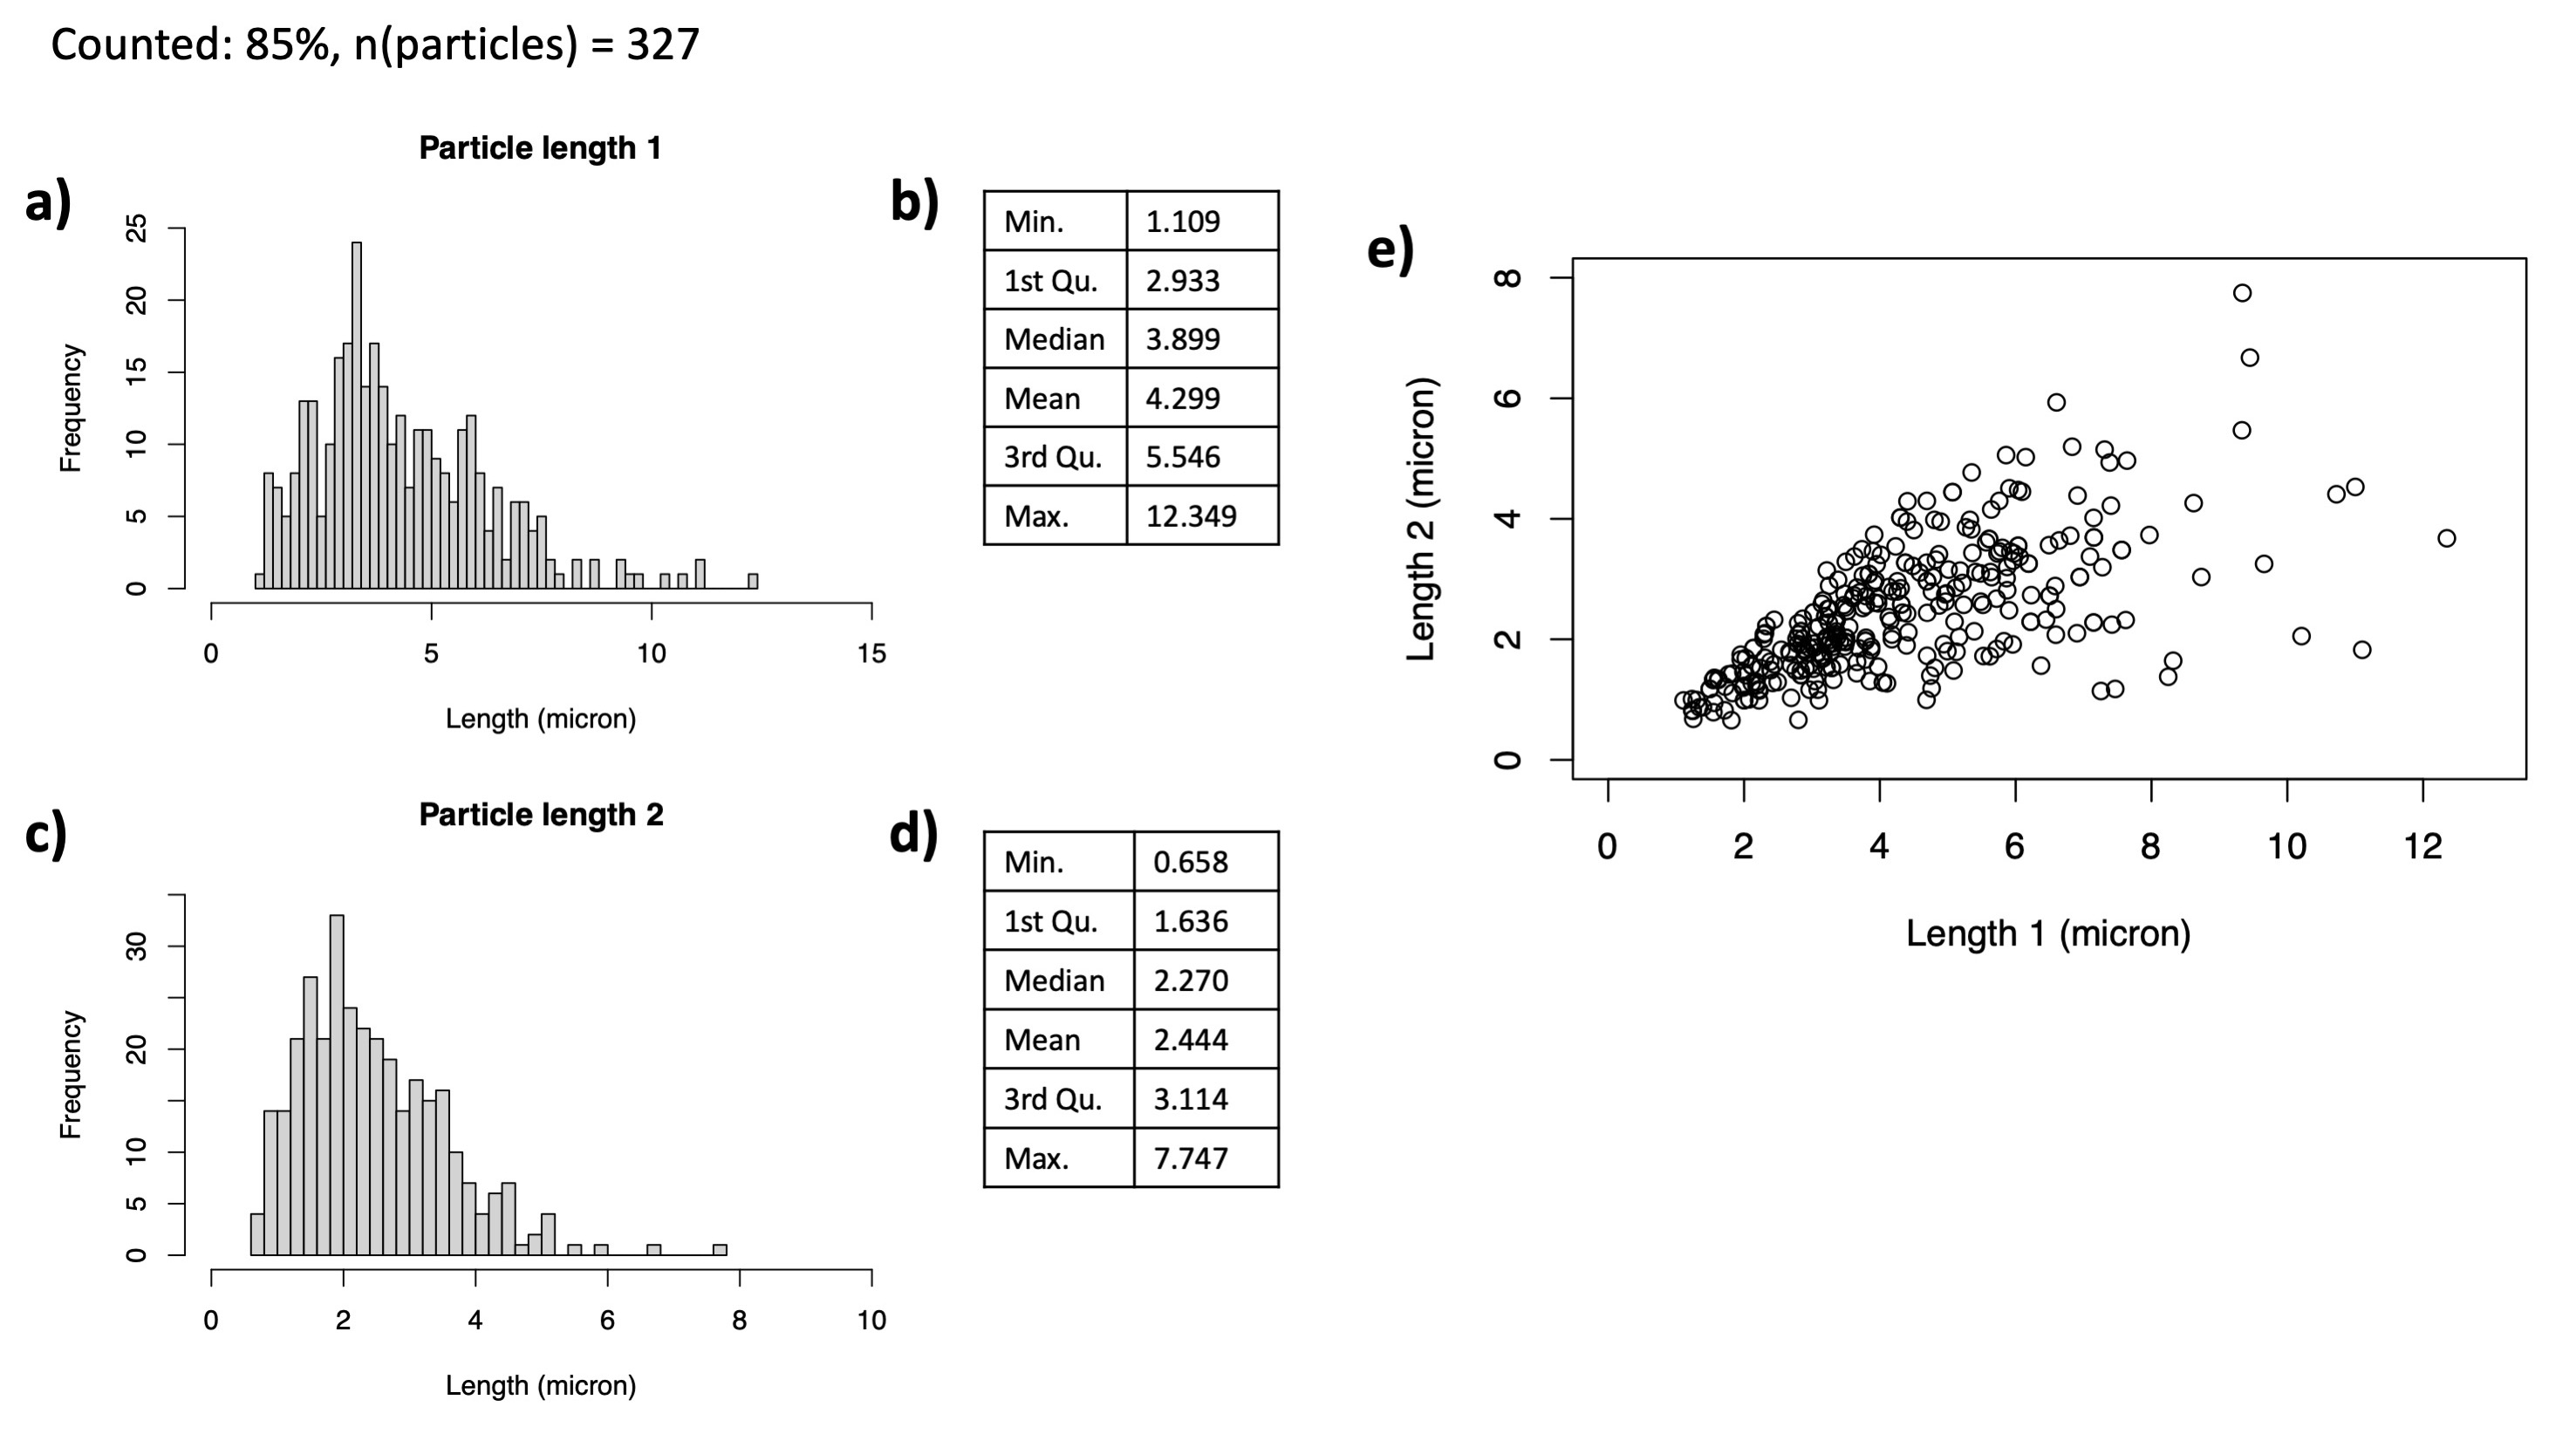
\includegraphics[width=0.8\linewidth]{1259.28_partsize}
\caption[Particle size distribution, sample 1259.28.]{Particle size distribution of sample 1259.28: \textbf{a)} Histogram showing distribution of particle length 1 values. \textbf{b)} Descriptive statistics for particle length 1 data. \textbf{c)} Histogram showing distribution of particle length 2 values. \textbf{d)} Descriptive statistics for particle length 2 data. \textbf{e)} Graph of length 1 versus length 2 showing the degree of skew.}
\label{fig:1259.28_partsize}
\end{figure}


\section{Sample 1259.29}

\begin{figure}[H]
  \centering
  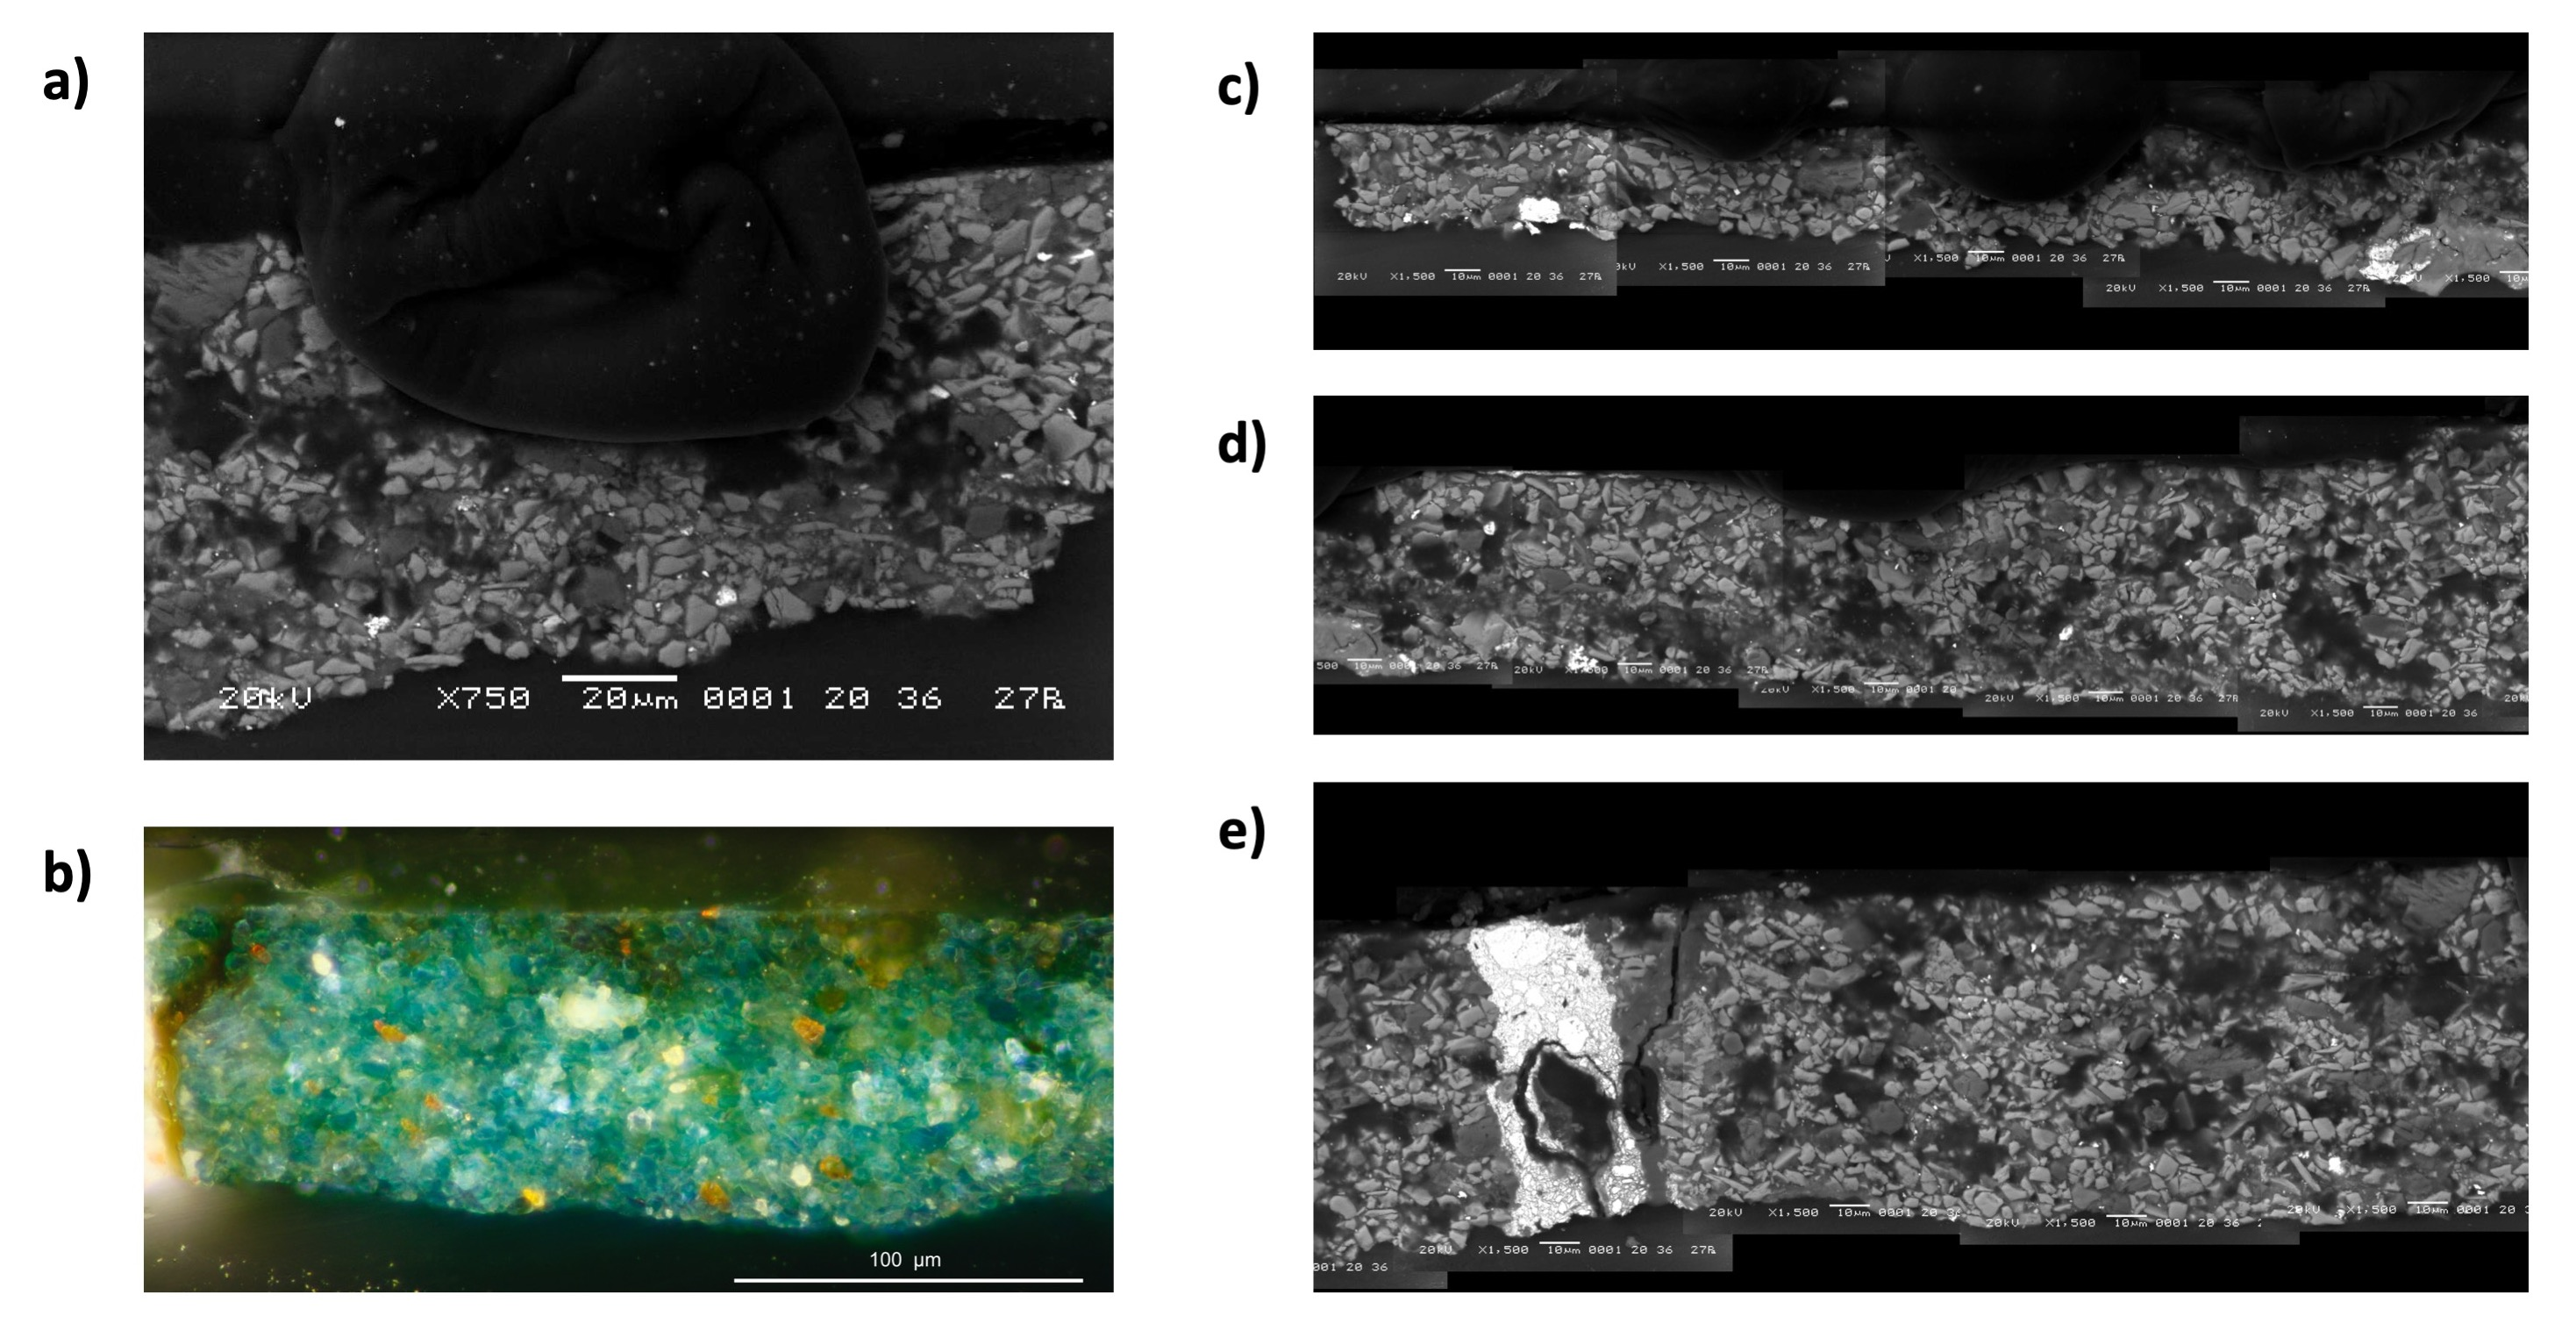
\includegraphics[width=0.8\linewidth]{1259.29_imgs}
\caption[SEM and dark field images of sample 1259.29.]{SEM and dark field images of sample 1259.29: \textbf{a)} 750x magnification, \textbf{b)} dark field microscope image of sample, \textbf{c-e)} 1500x magnification composite image of entire sample region. The dark blobs on sample surface in SEM images are resin patches (and are transparent in dark field images). Dark field microscope images courtesy of Katharine Waldron, HKI.}
\label{fig:1259.29_imgs}
\end{figure}

\begin{figure}[H]
\centering
\begin{minipage}[t]{\linewidth}
  \centering
  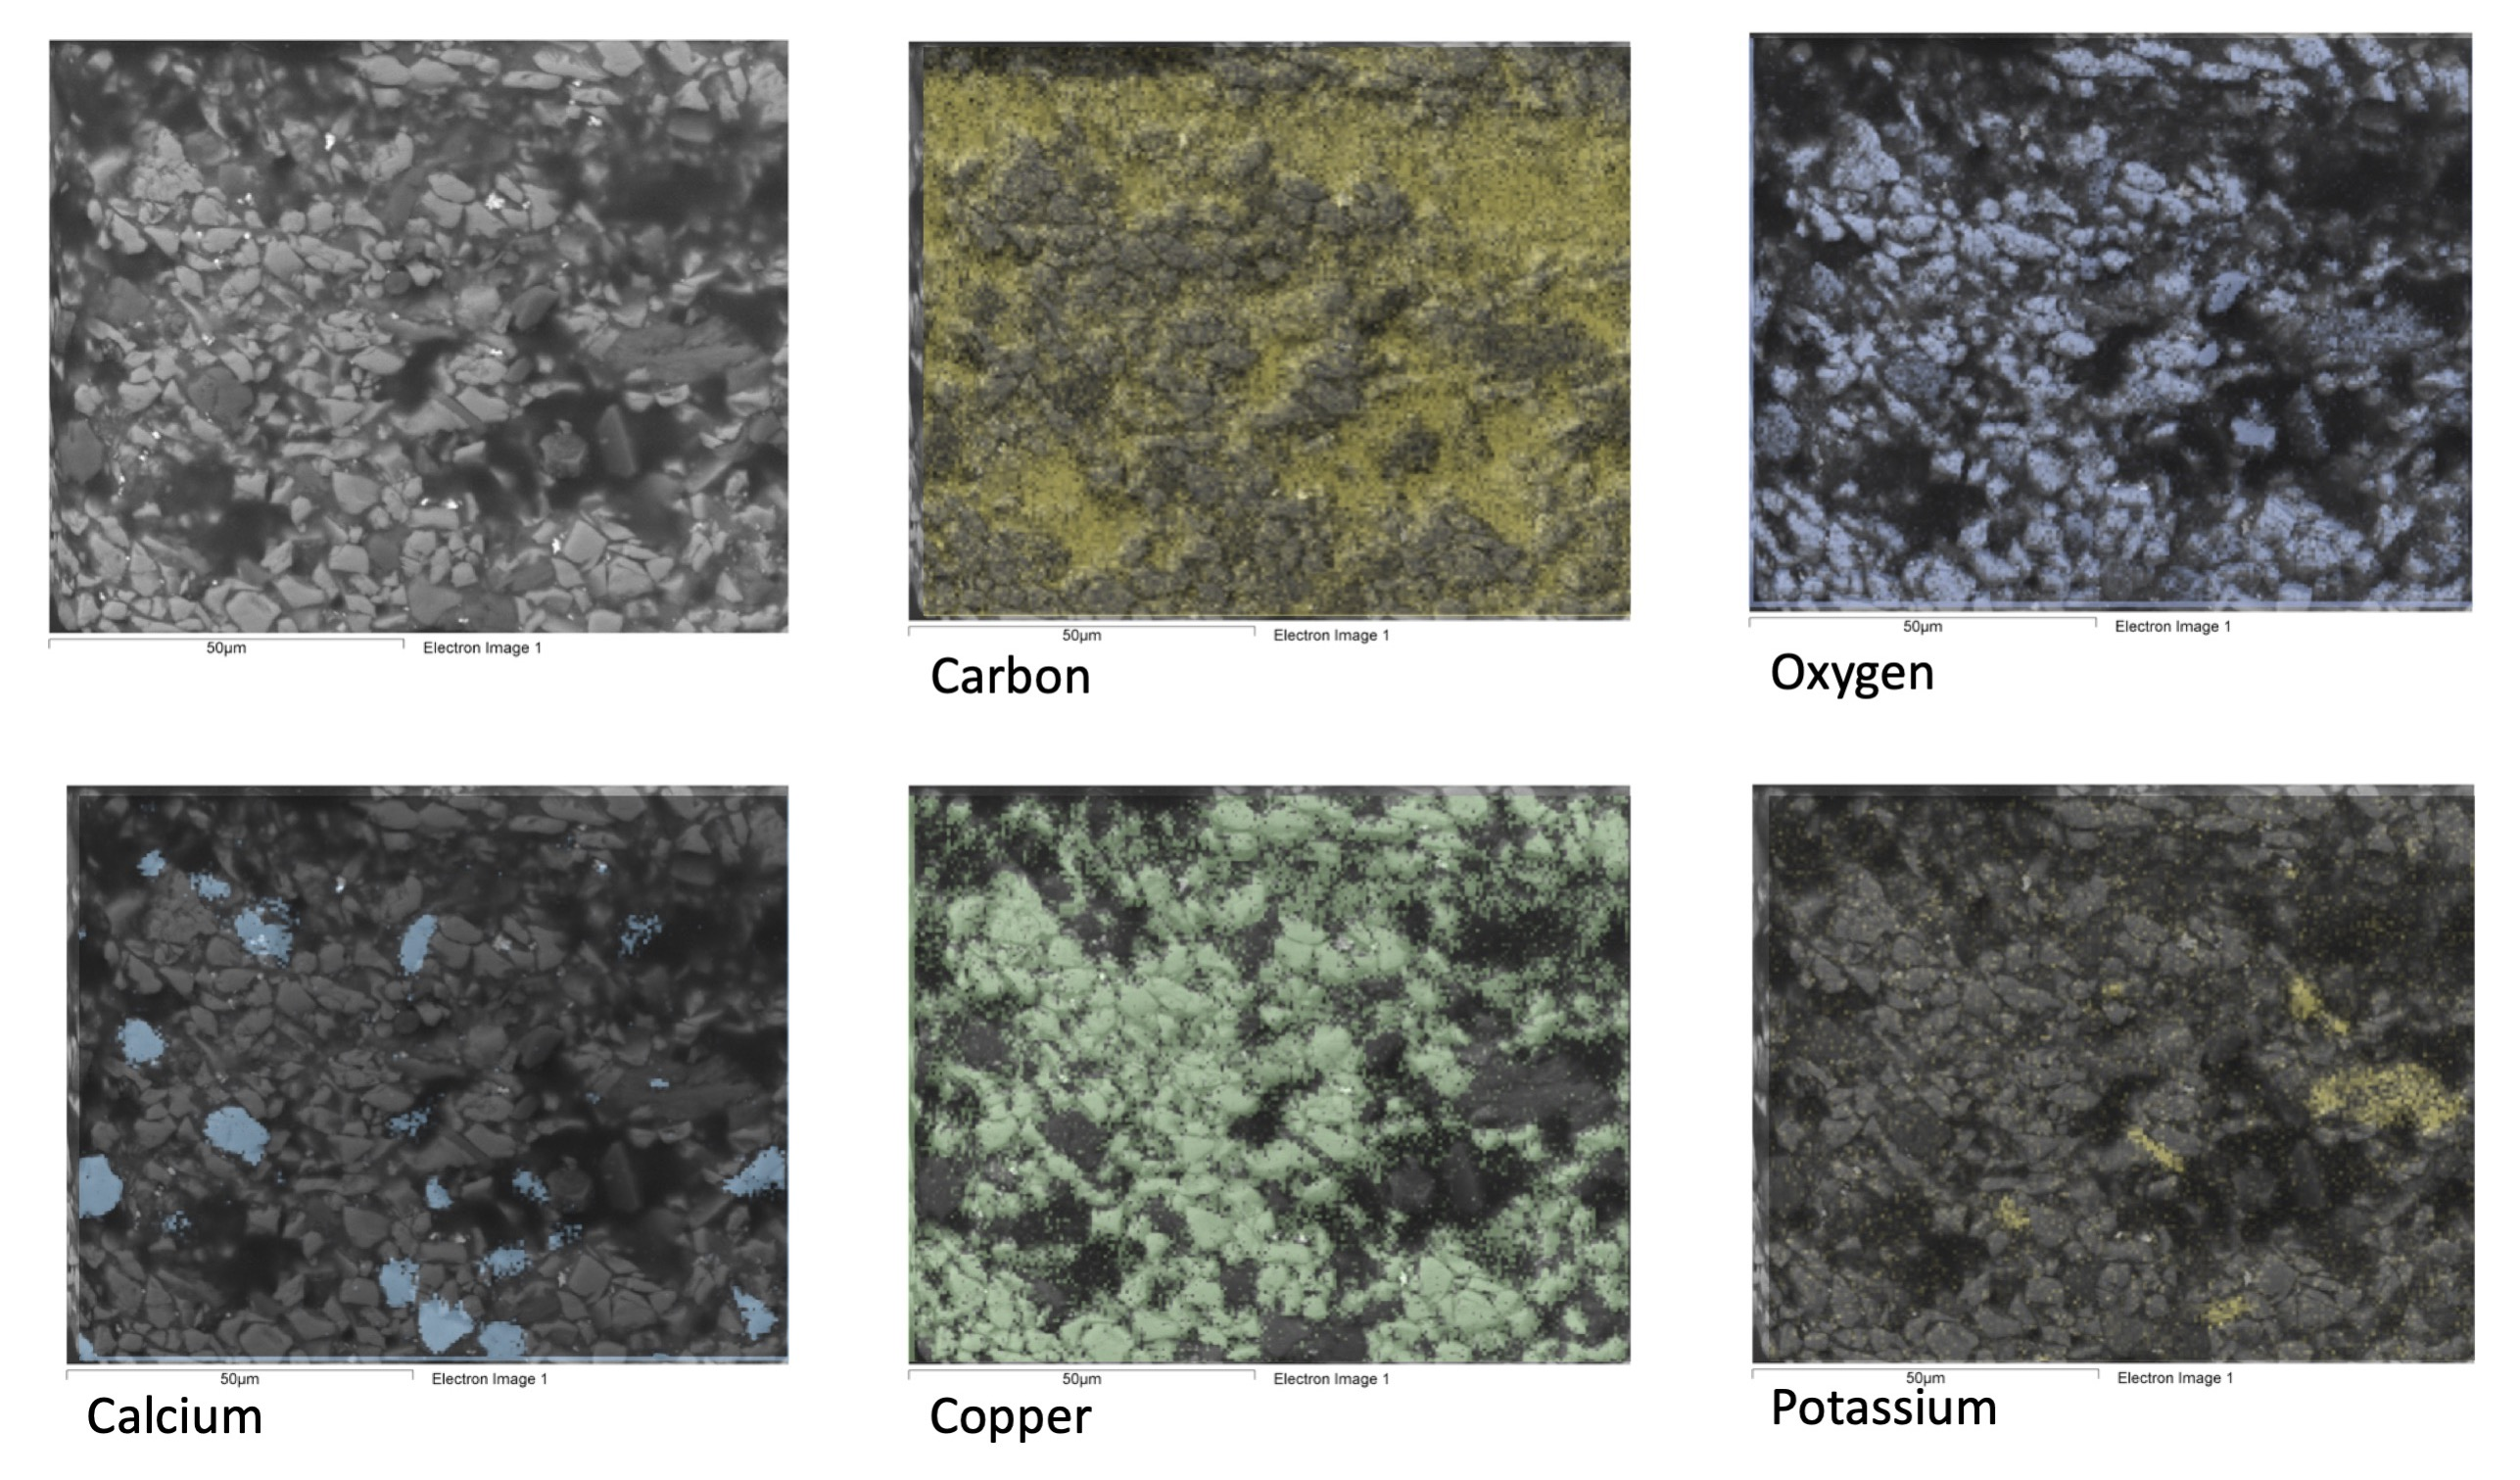
\includegraphics[width=0.9\linewidth]{1259.29_mapdata_1}
\hfill
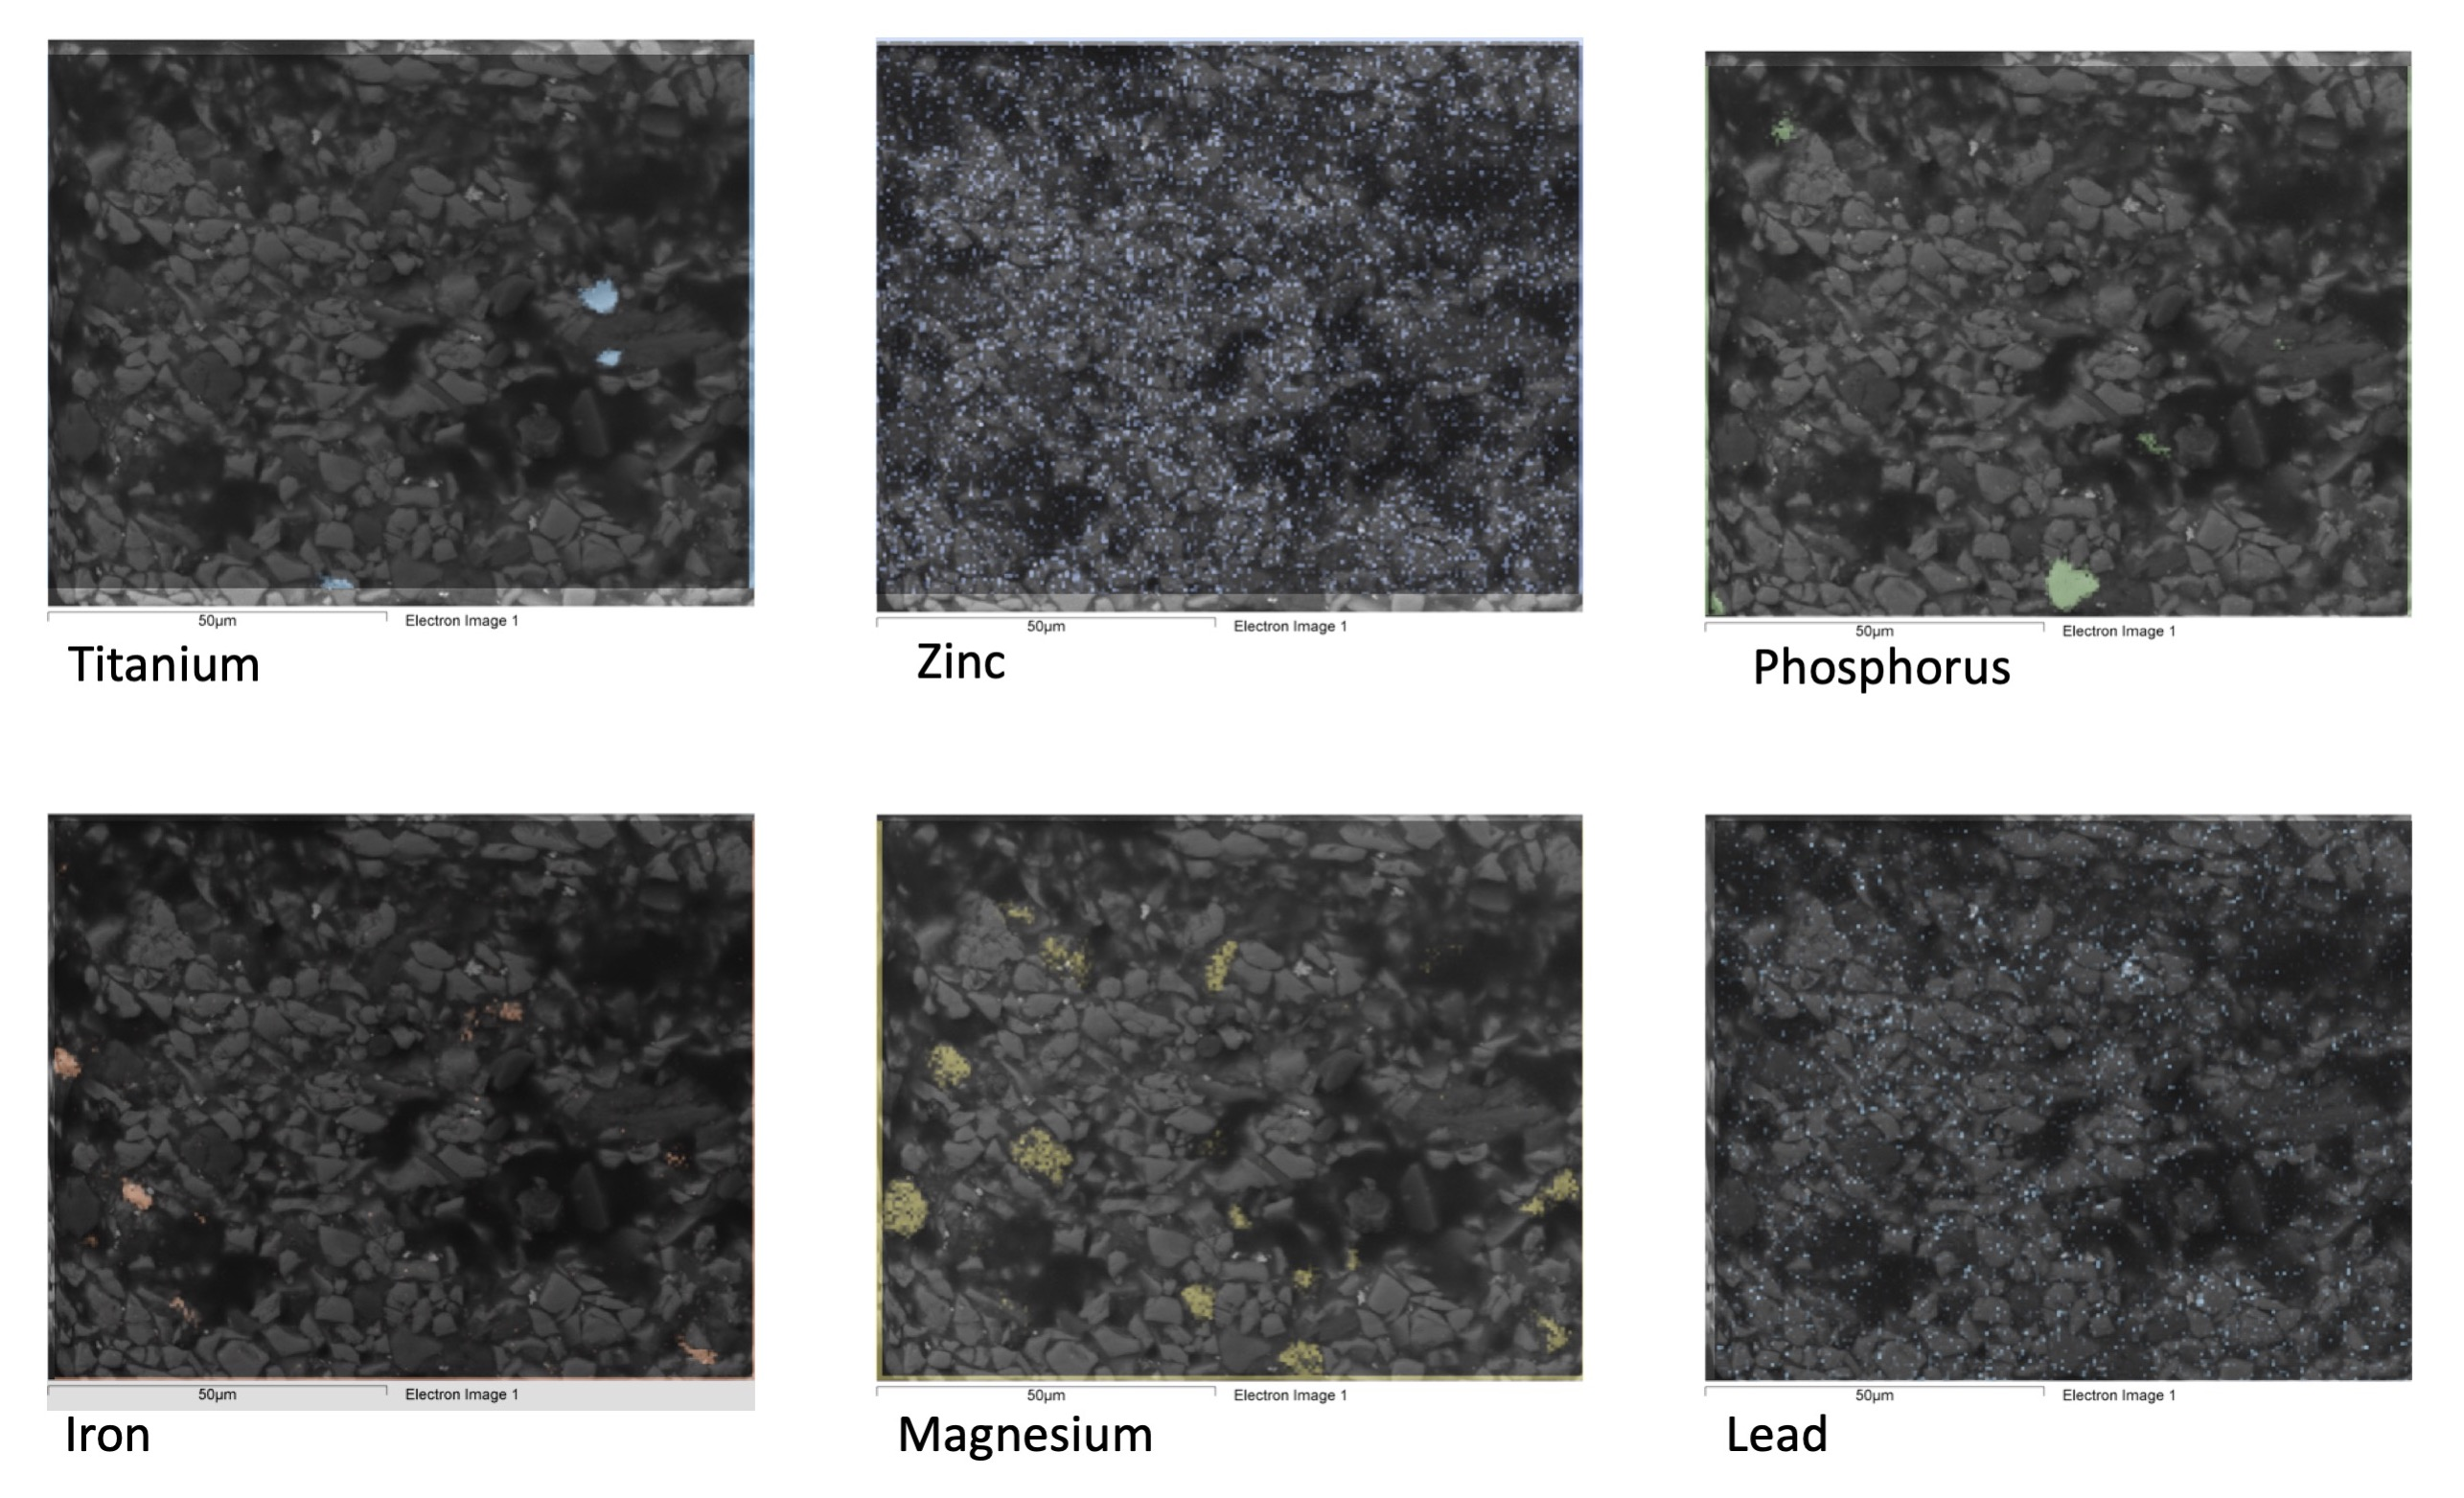
\includegraphics[width=0.9\linewidth]{1259.29_mapdata_2}
\hfill
\end{minipage}
\caption[EDS map data, sample 1259.29.]{EDS map data of sample 1259.29 showing locations of elements in an area of the azurite paint layer. Elements detected are C, O, Ca, Cu, K, Ti, Zn, P, Fe, Mg, and Pb.}
\label{fig:1259.29_mapdata}
\end{figure}


\begin{figure}[H]
\centering
  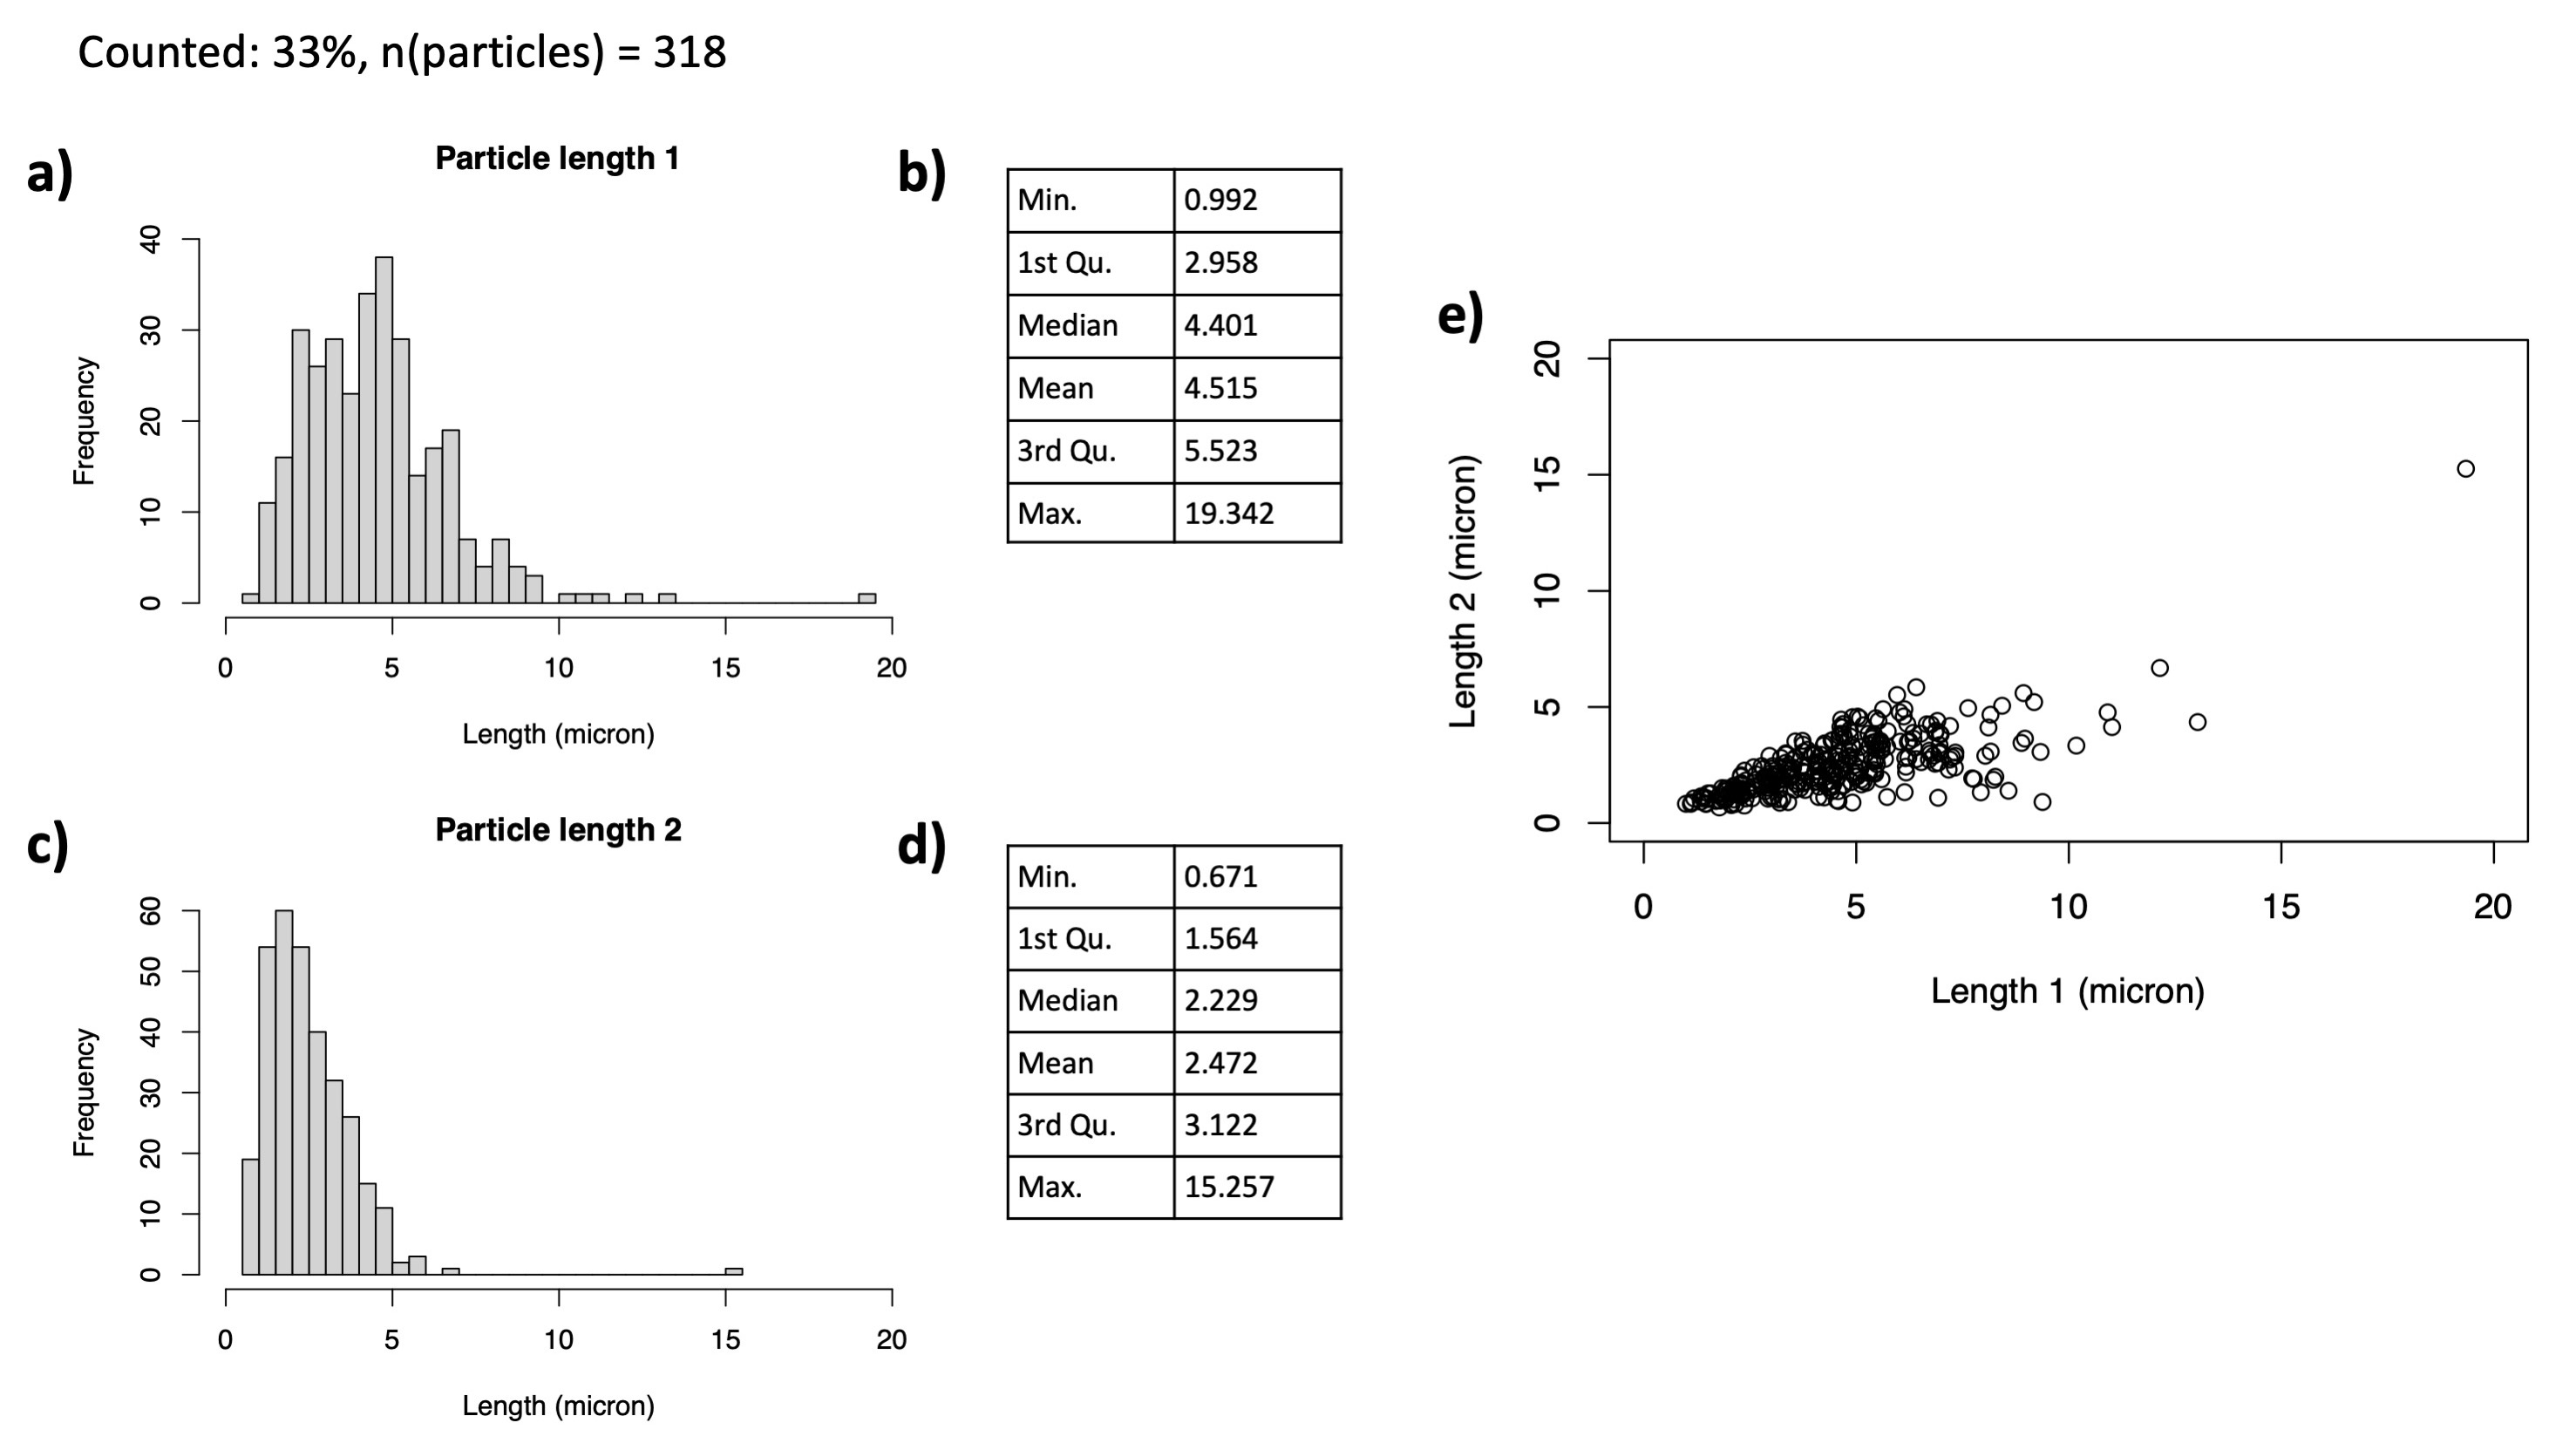
\includegraphics[width=0.8\linewidth]{1259.29_partsize}
\caption[Particle size distribution, sample 1259.29.]{Particle size distribution of sample 1259.29: \textbf{a)} Histogram showing distribution of particle length 1 values. \textbf{b)} Descriptive statistics for particle length 1 data. \textbf{c)} Histogram showing distribution of particle length 2 values. \textbf{d)} Descriptive statistics for particle length 2 data. \textbf{e)} Graph of length 1 versus length 2 showing the degree of skew.}
\label{fig:1259.29_partsize}
\end{figure}


\section{Sample 1259.33}

\textit{Figure \ref{fig:1259.33_imgs}} shows SEM and dark field microscope images of 1259.33. Two azurite-containing layers are present, more clearly differentiable in the dark field image. \textit{Figure \ref{fig:1259.33_pointspec}} addresses elemental variation between these two layers. The top layer has a Cu:O ratio of 0.271, while the bottom layer has a Cu:O ratio of 0.366. A particle selected at the boundary of these layers fits well with the chemical composition of the top layer. 

EDS maps of 1259.33 are shown in \textit{Figure \ref{fig:1259.33_mapdata}}, and based on elemental correlations, the following compounds are present: azurite, magnesium containing aluminosilicates, calcium phosphate, and lead (likely lead white). Iron is not detected at significant levels.

The particle size distribution is similar between the bottom and top layers, shown in \textit{Figures \ref{fig:1259.33_partsize_1}} and \textit{\ref{fig:1259.33_partsize_2}}. The bottom layer shows a slightly larger average particle size due to outlier data points.

\begin{figure}[H]
  \centering
  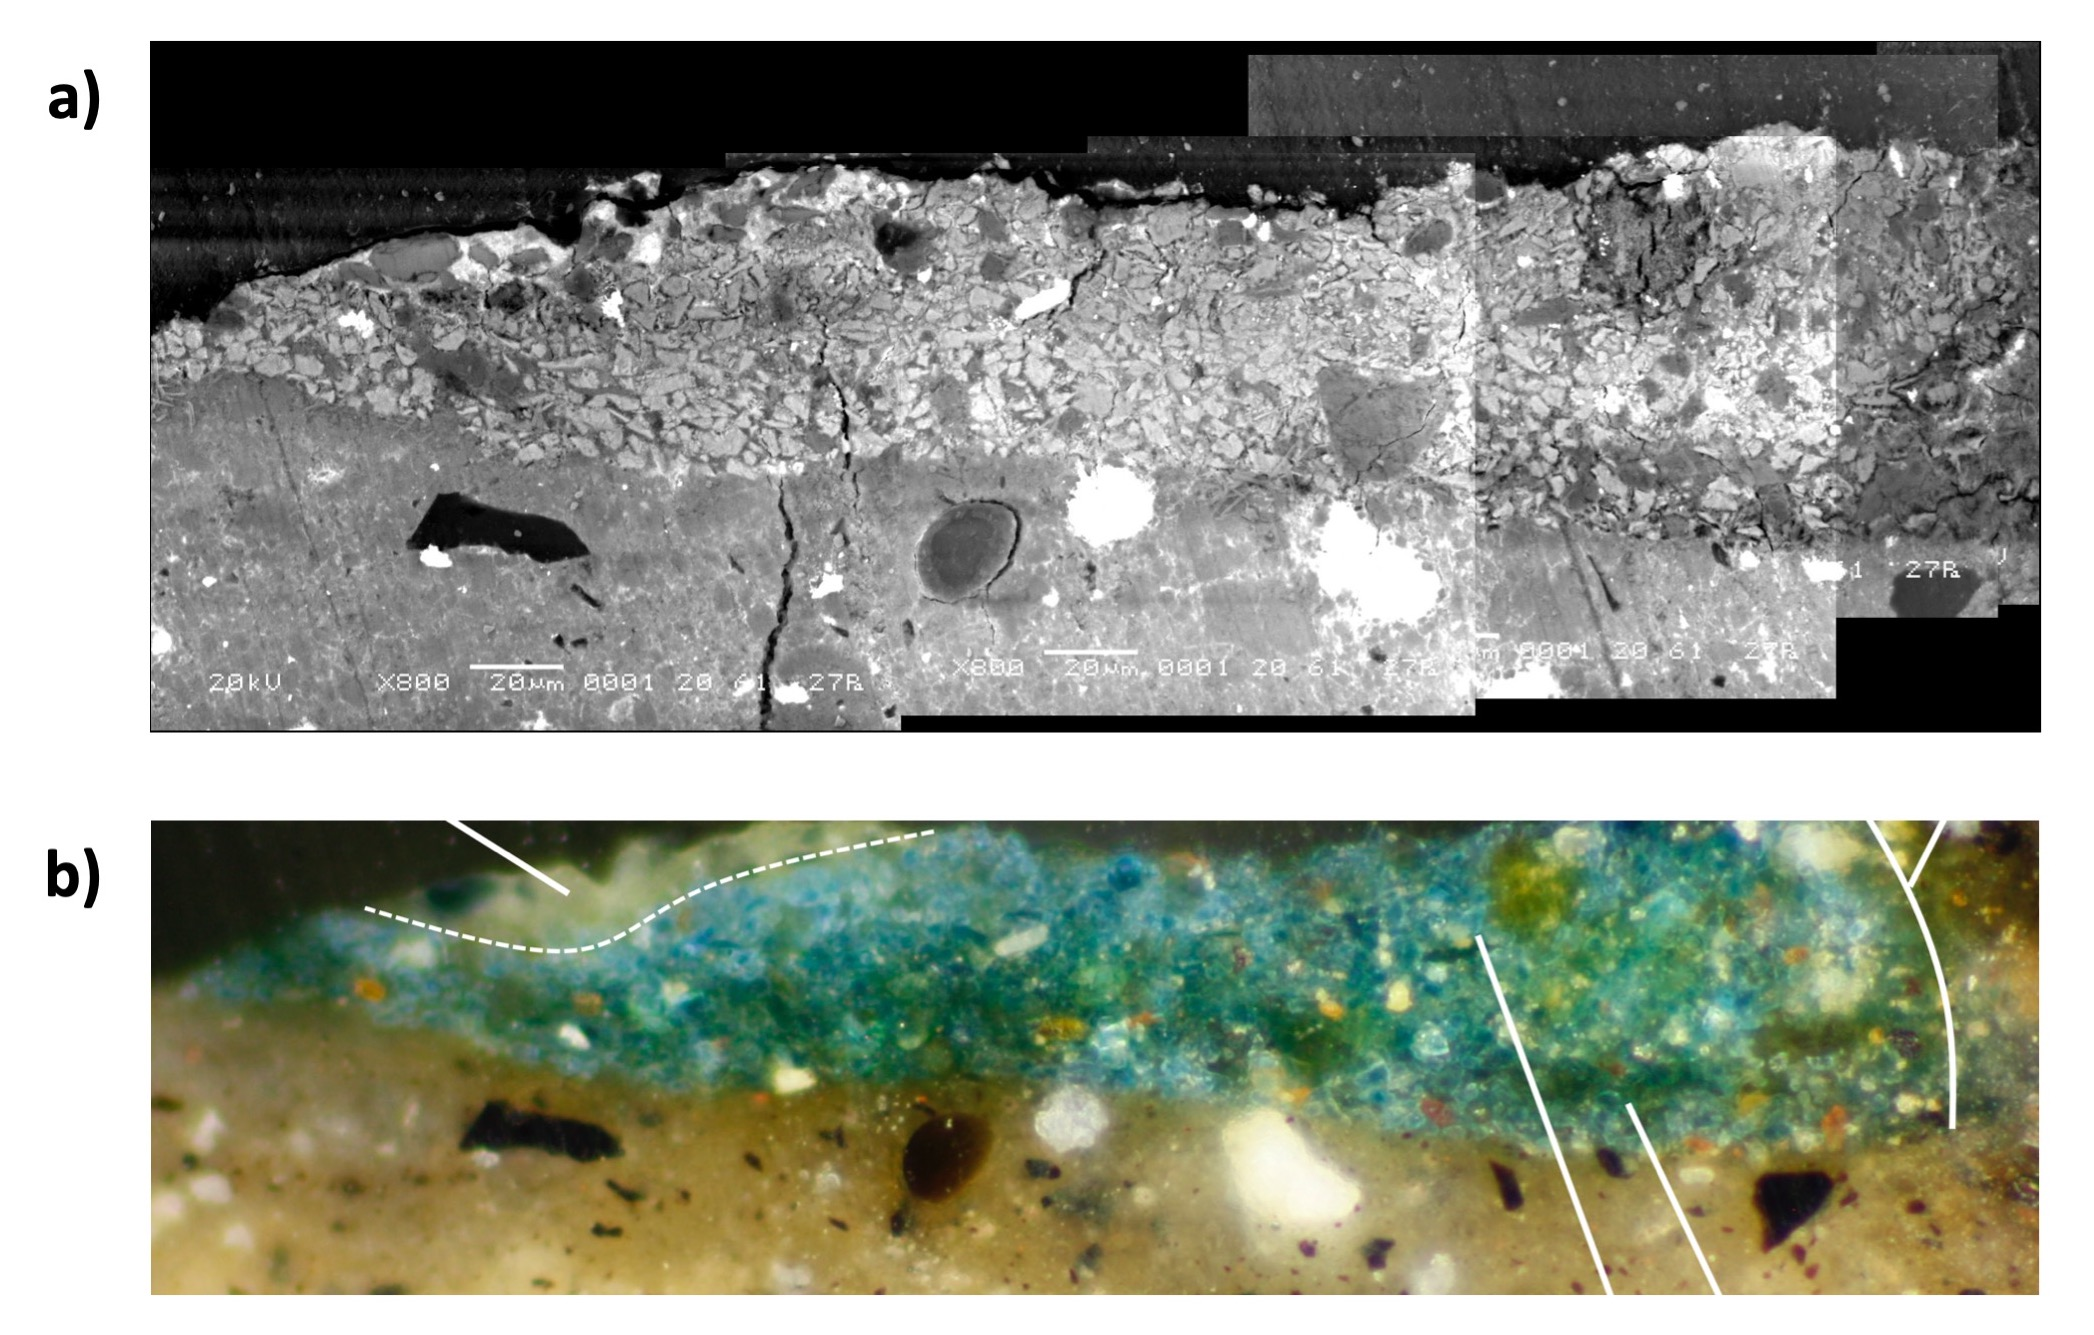
\includegraphics[width=0.8\linewidth]{1259.33_imgs}
\caption[SEM and dark field images of sample 1259.33.]{SEM and dark field images of sample 1259.33: \textbf{a)} composite image of azurite containing layers, 800x magnification, \textbf{b)} dark field microscope image of cross section. Dark field microscope images courtesy of Katharine Waldron, HKI.}
\label{fig:1259.33_imgs}
\end{figure}

\begin{figure}[H]
  \centering
  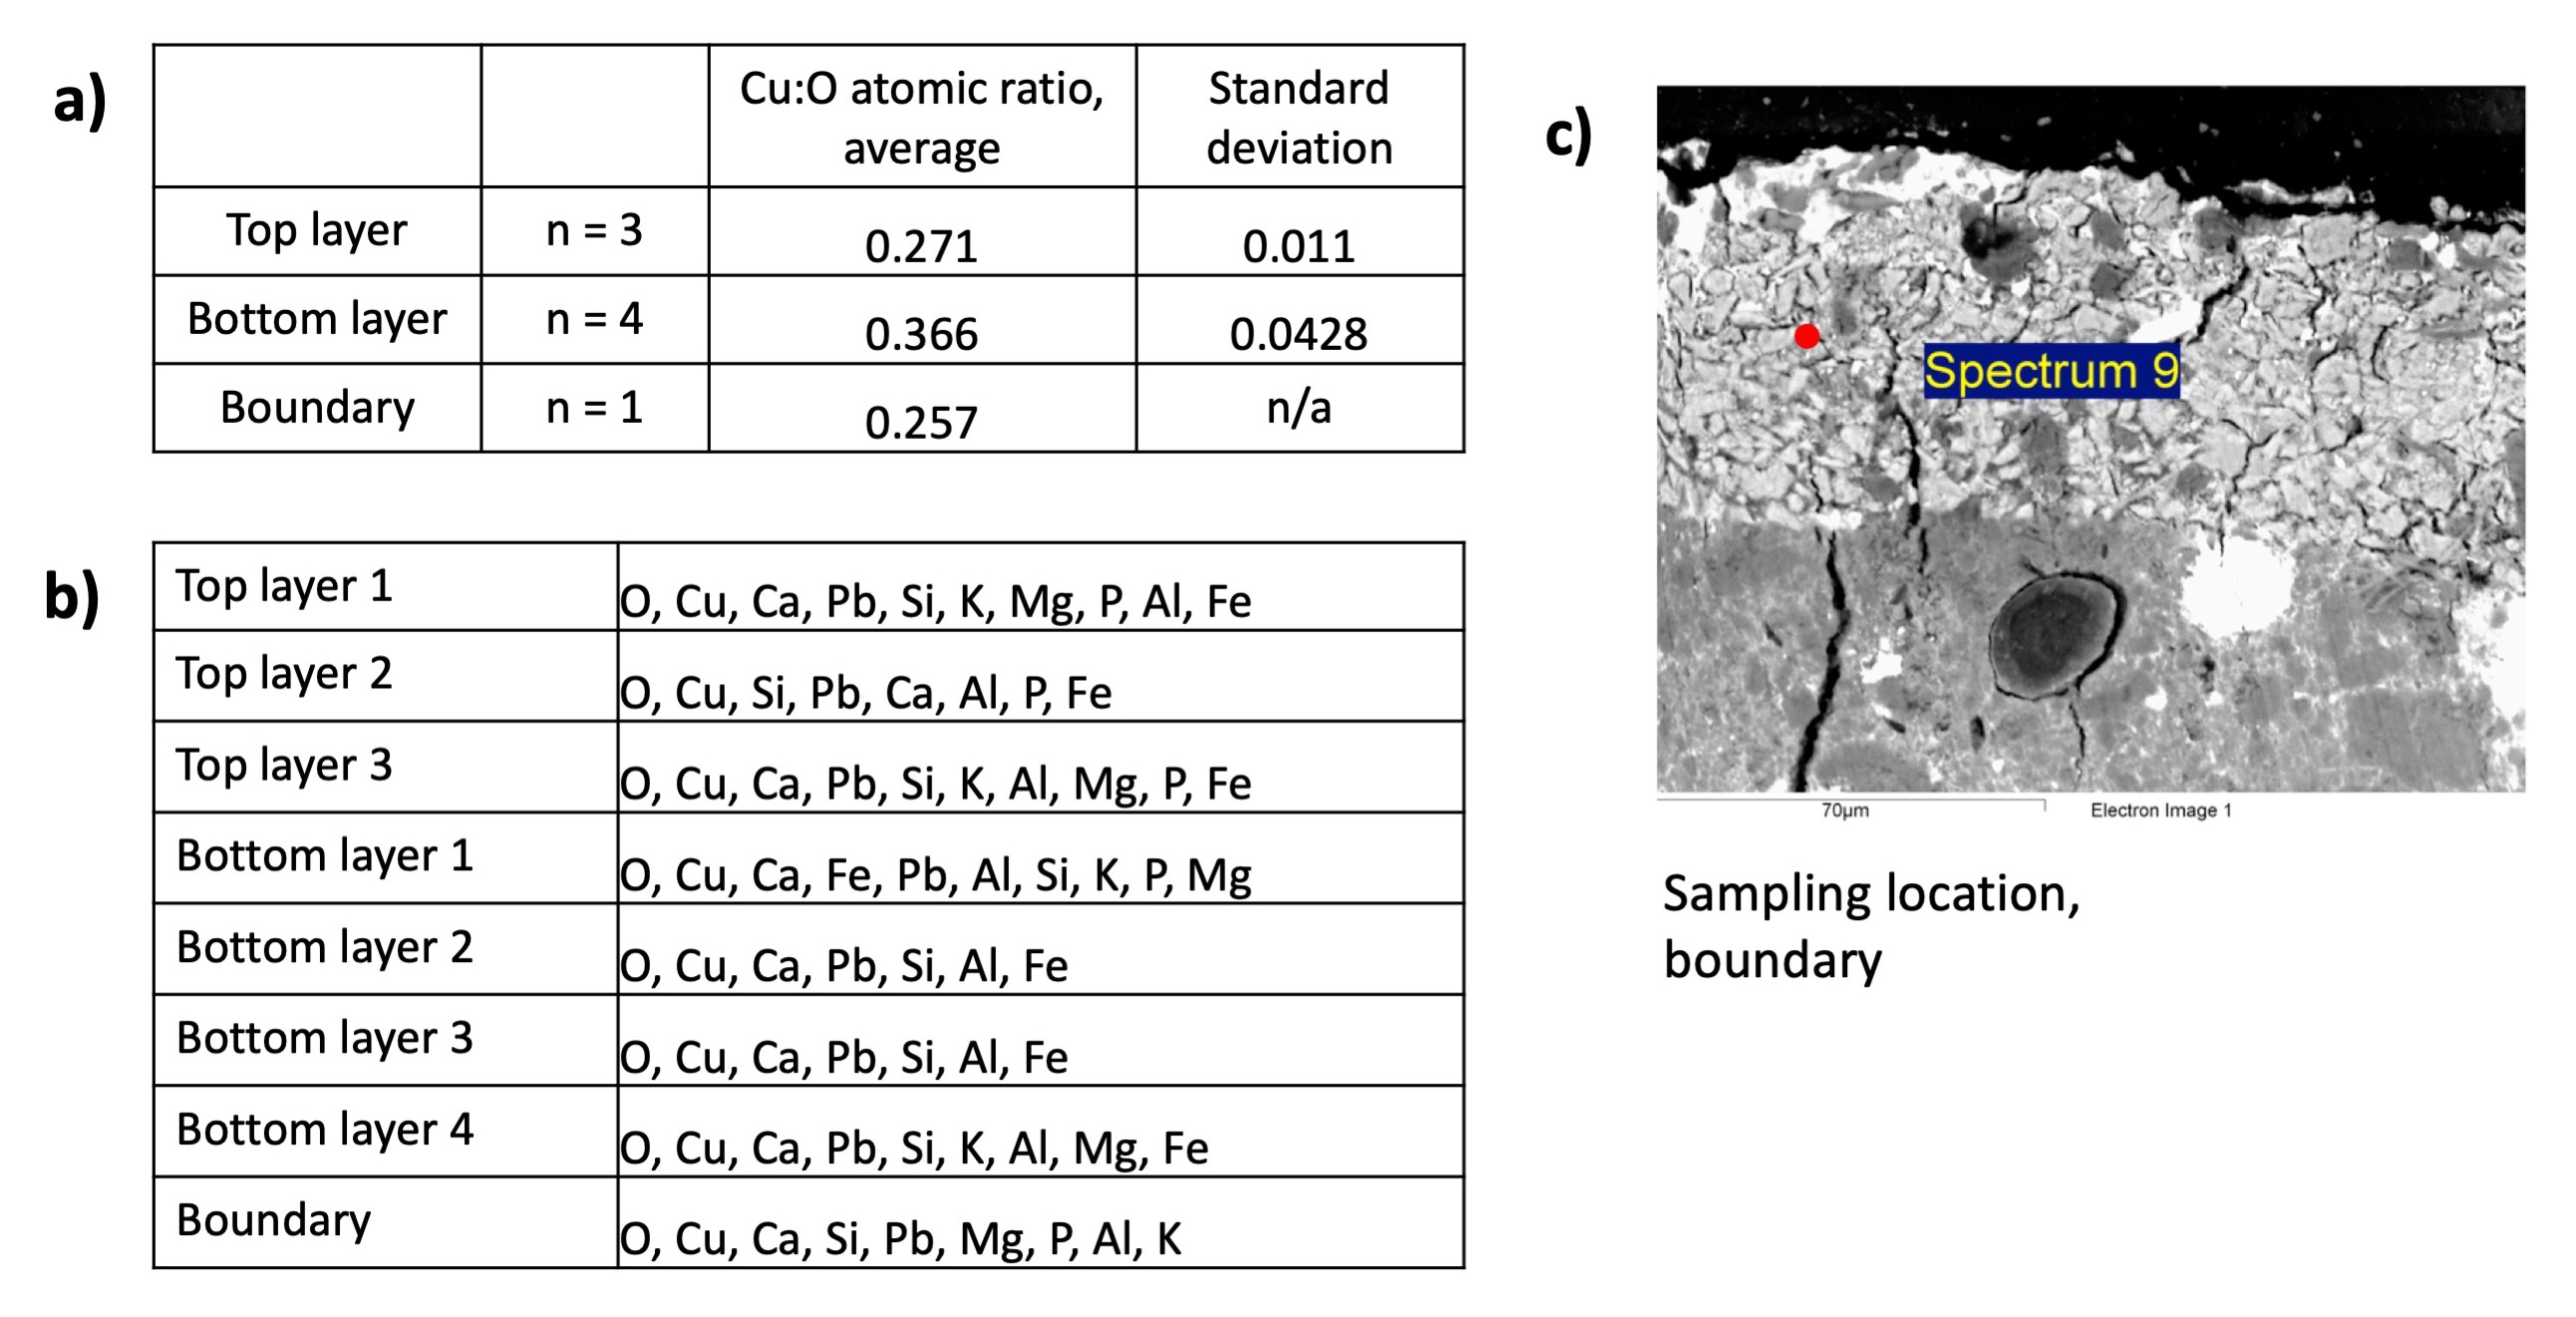
\includegraphics[width=0.8\linewidth]{1259.33_eds_pointspec}
\caption[EDS point spectrum data, sample 1259.33.]{EDS point spectrum data, sample 1259.33: \textbf{a)} quantitative EDS results showing average Cu:O ratio and standard deviation from point spectra collected from azurite particles from the two distinct paint layers in the sample. One sample from the layer boundary is also presented. \textbf{b)} table of elements detected in each point spectrum, \textbf{c)} SEM image showing point spectrum location of boundary sample. This data shows a consistent quantitative difference in the Cu:O ratio between azurite particles in the two paint layers.}
\label{fig:1259.33_pointspec}
\end{figure}

\begin{figure}[H]
\centering
\begin{minipage}[t]{\linewidth}
  \centering
  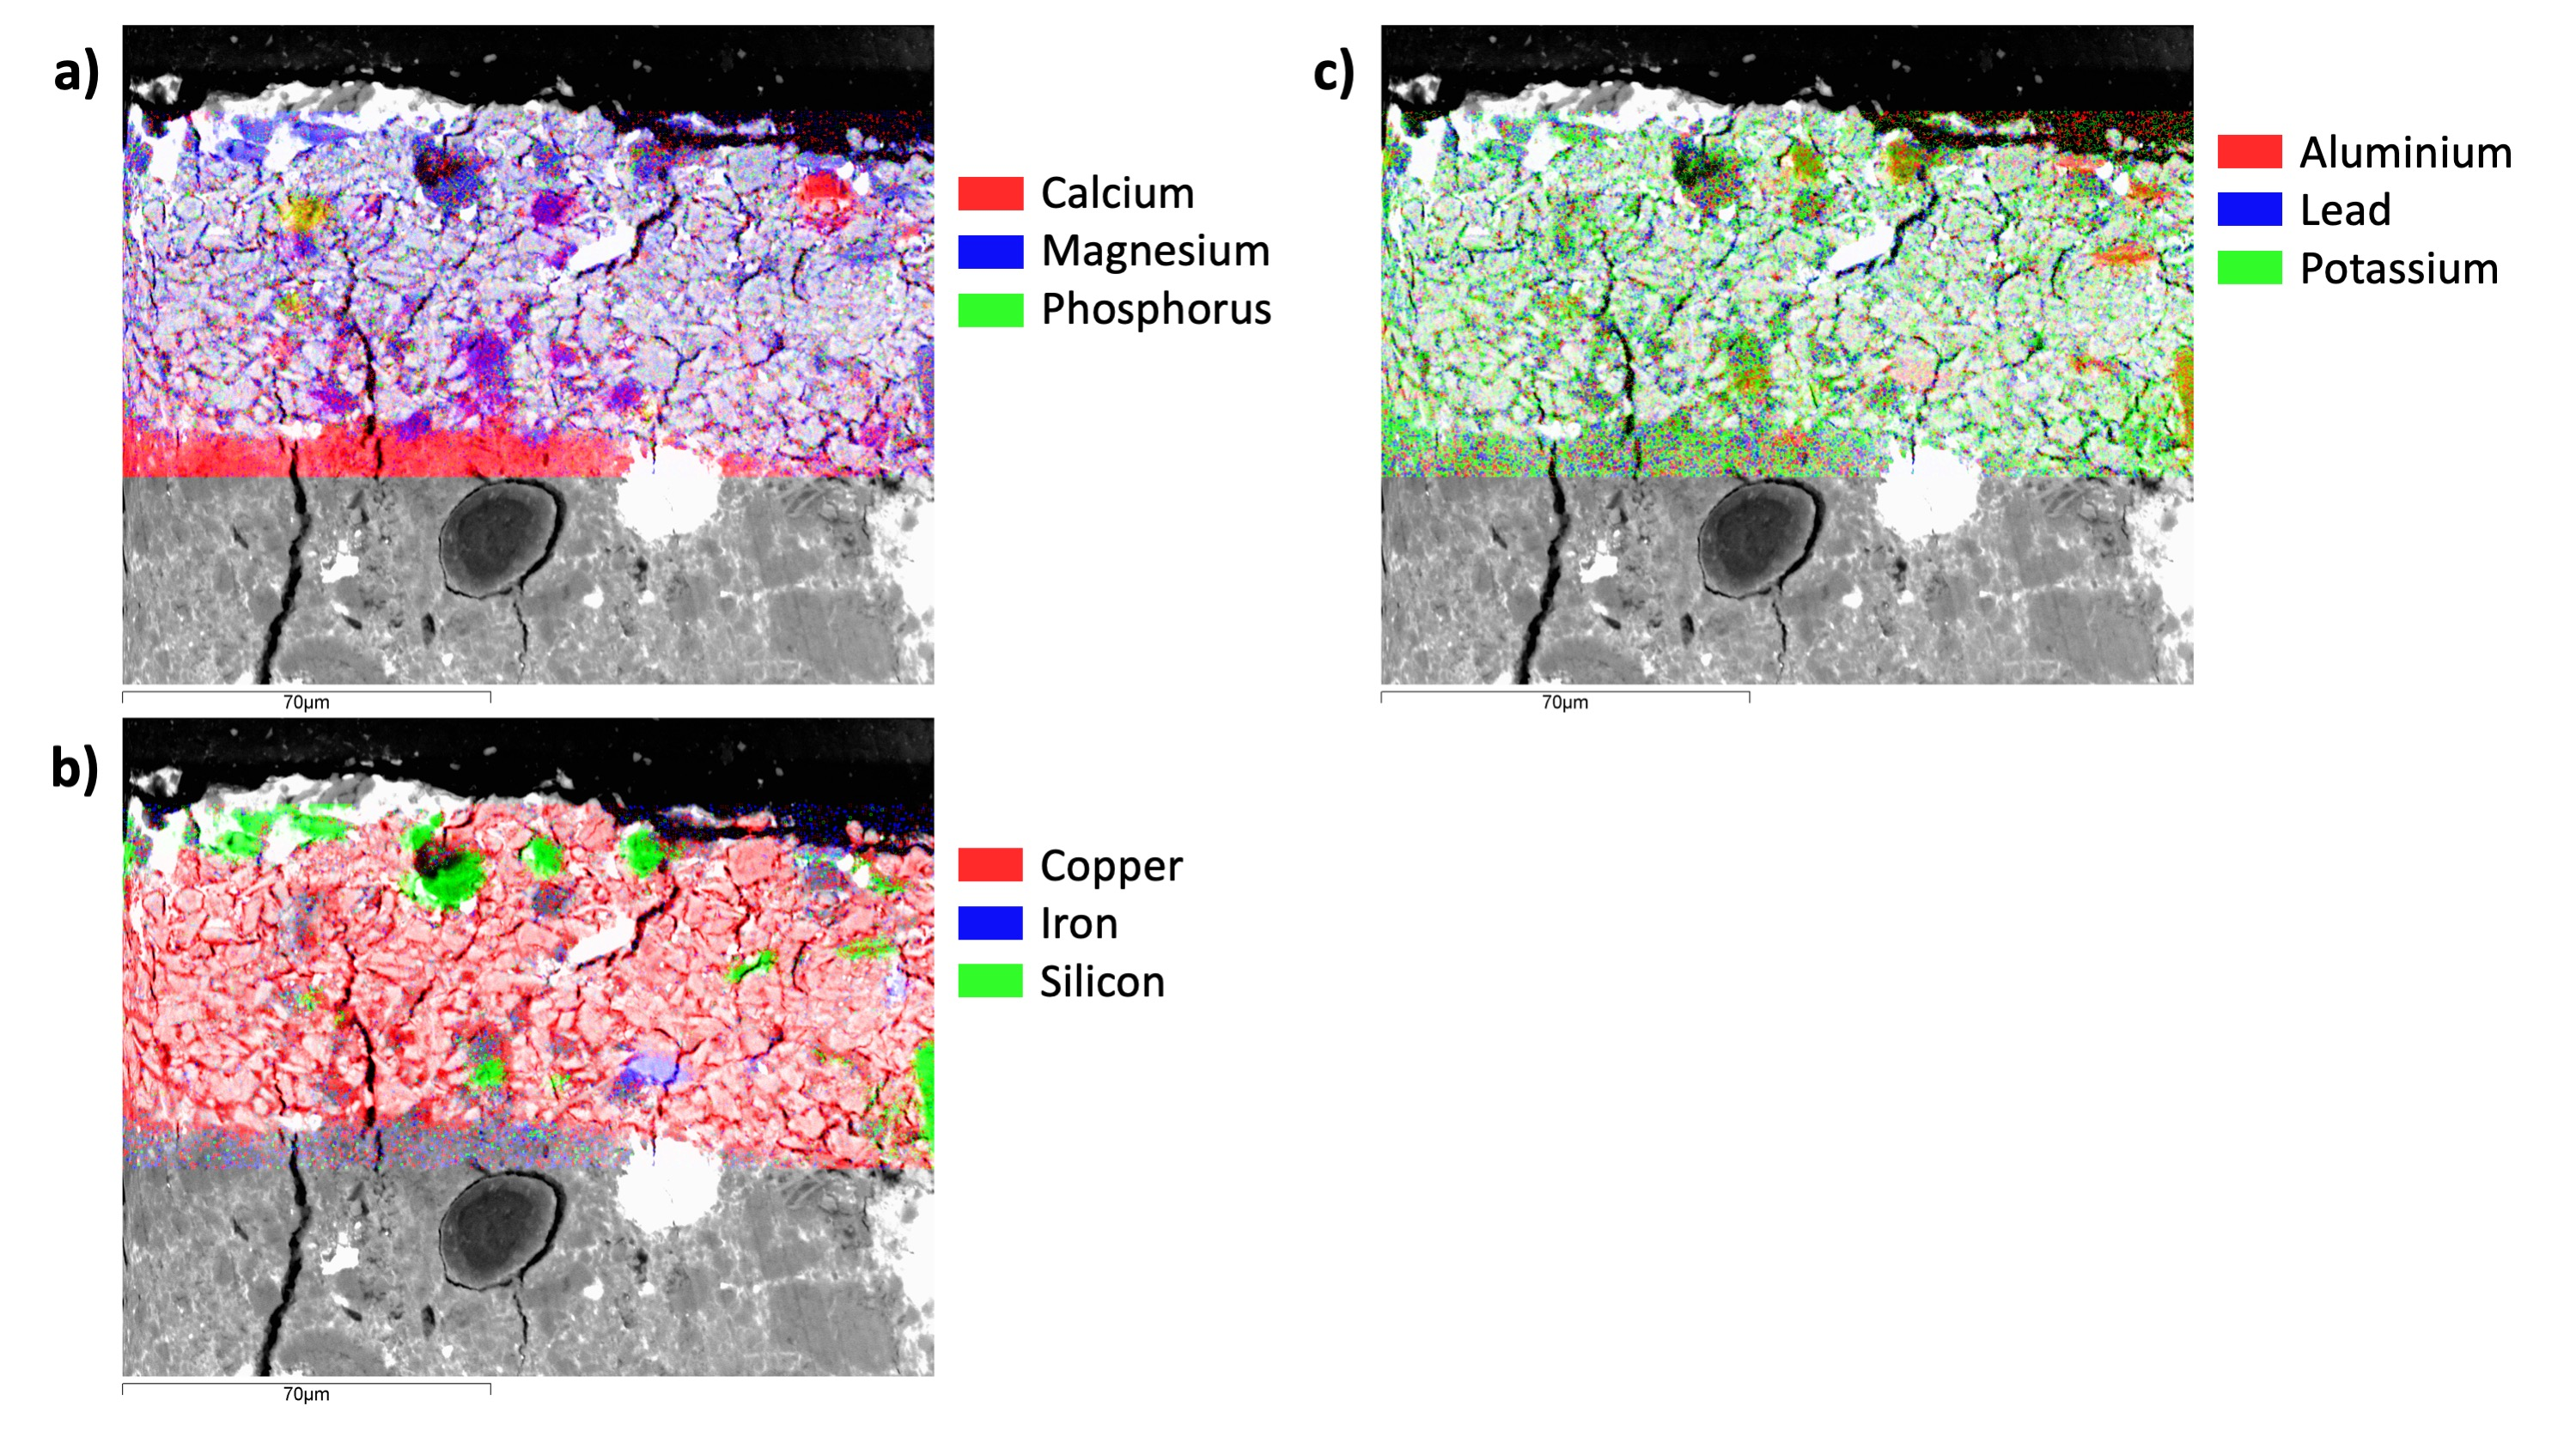
\includegraphics[width=0.9\linewidth]{1259.33_mapdata_1}
\hfill
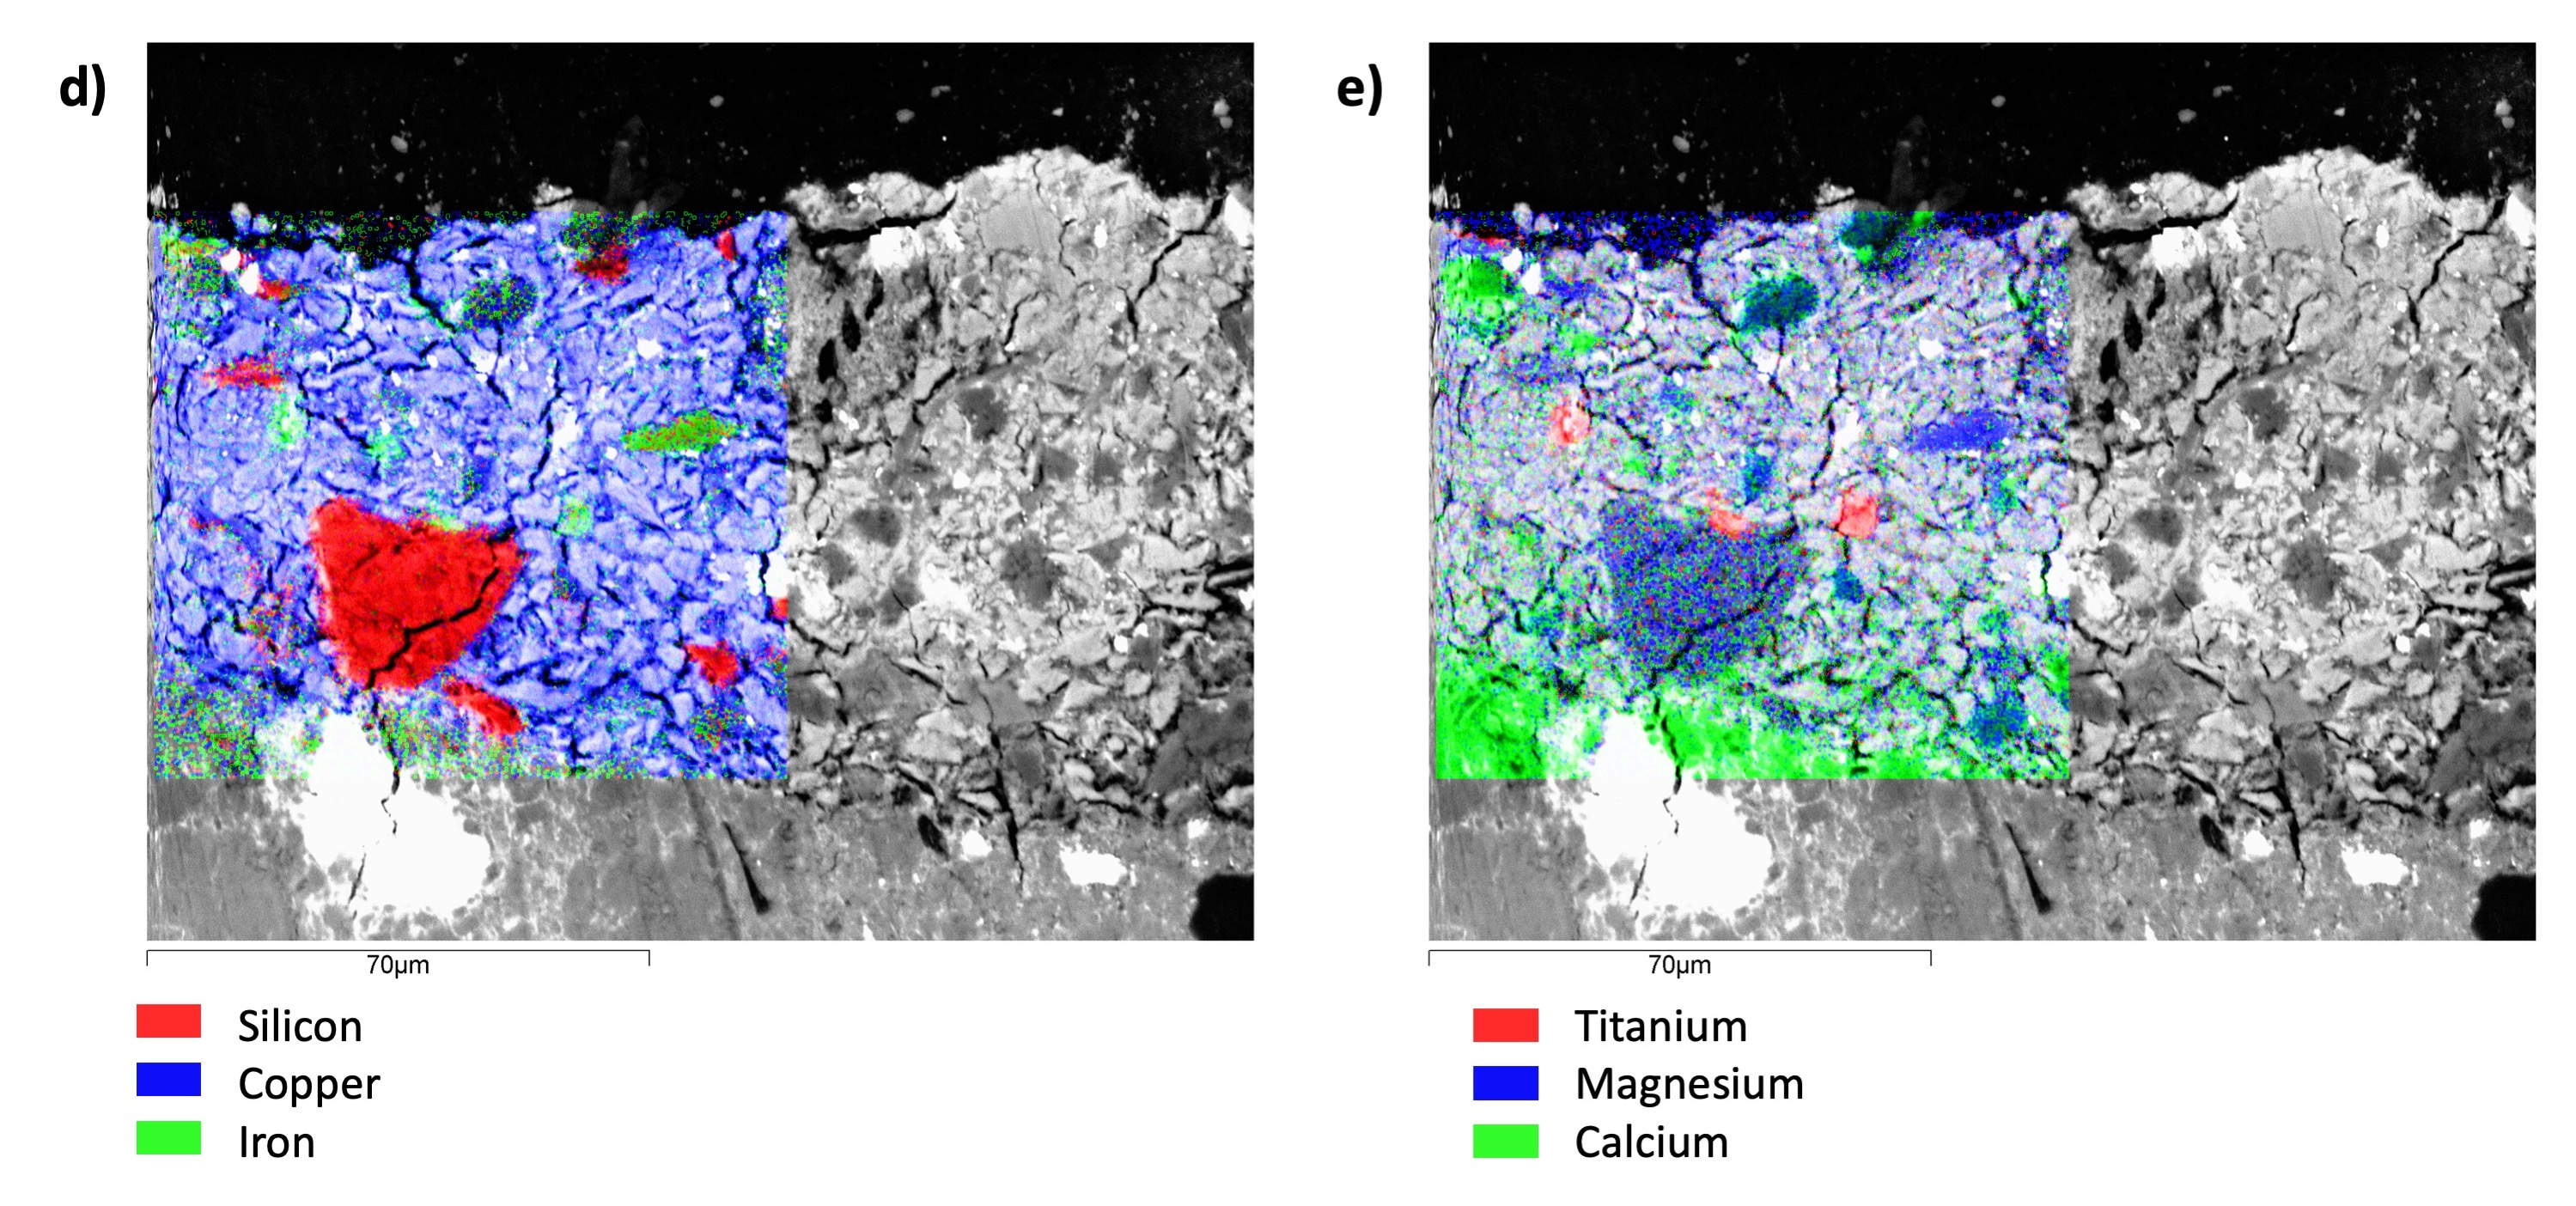
\includegraphics[width=0.9\linewidth]{1259.33_mapdata_2}
\hfill
\end{minipage}
\caption[EDS map data, sample 1259.33.]{EDS map data of sample 1259.33: \textbf{a-c)} elements detected in this region are Ca, Mg, P, Cu, Fe, Si, Al, Pb, K, \textbf{d, e)} elements detected in this region are Si, Cu, Fe, Ti, Mg, Ca.}
\label{fig:1259.33_mapdata}
\end{figure}

\begin{figure}[H]
\centering
  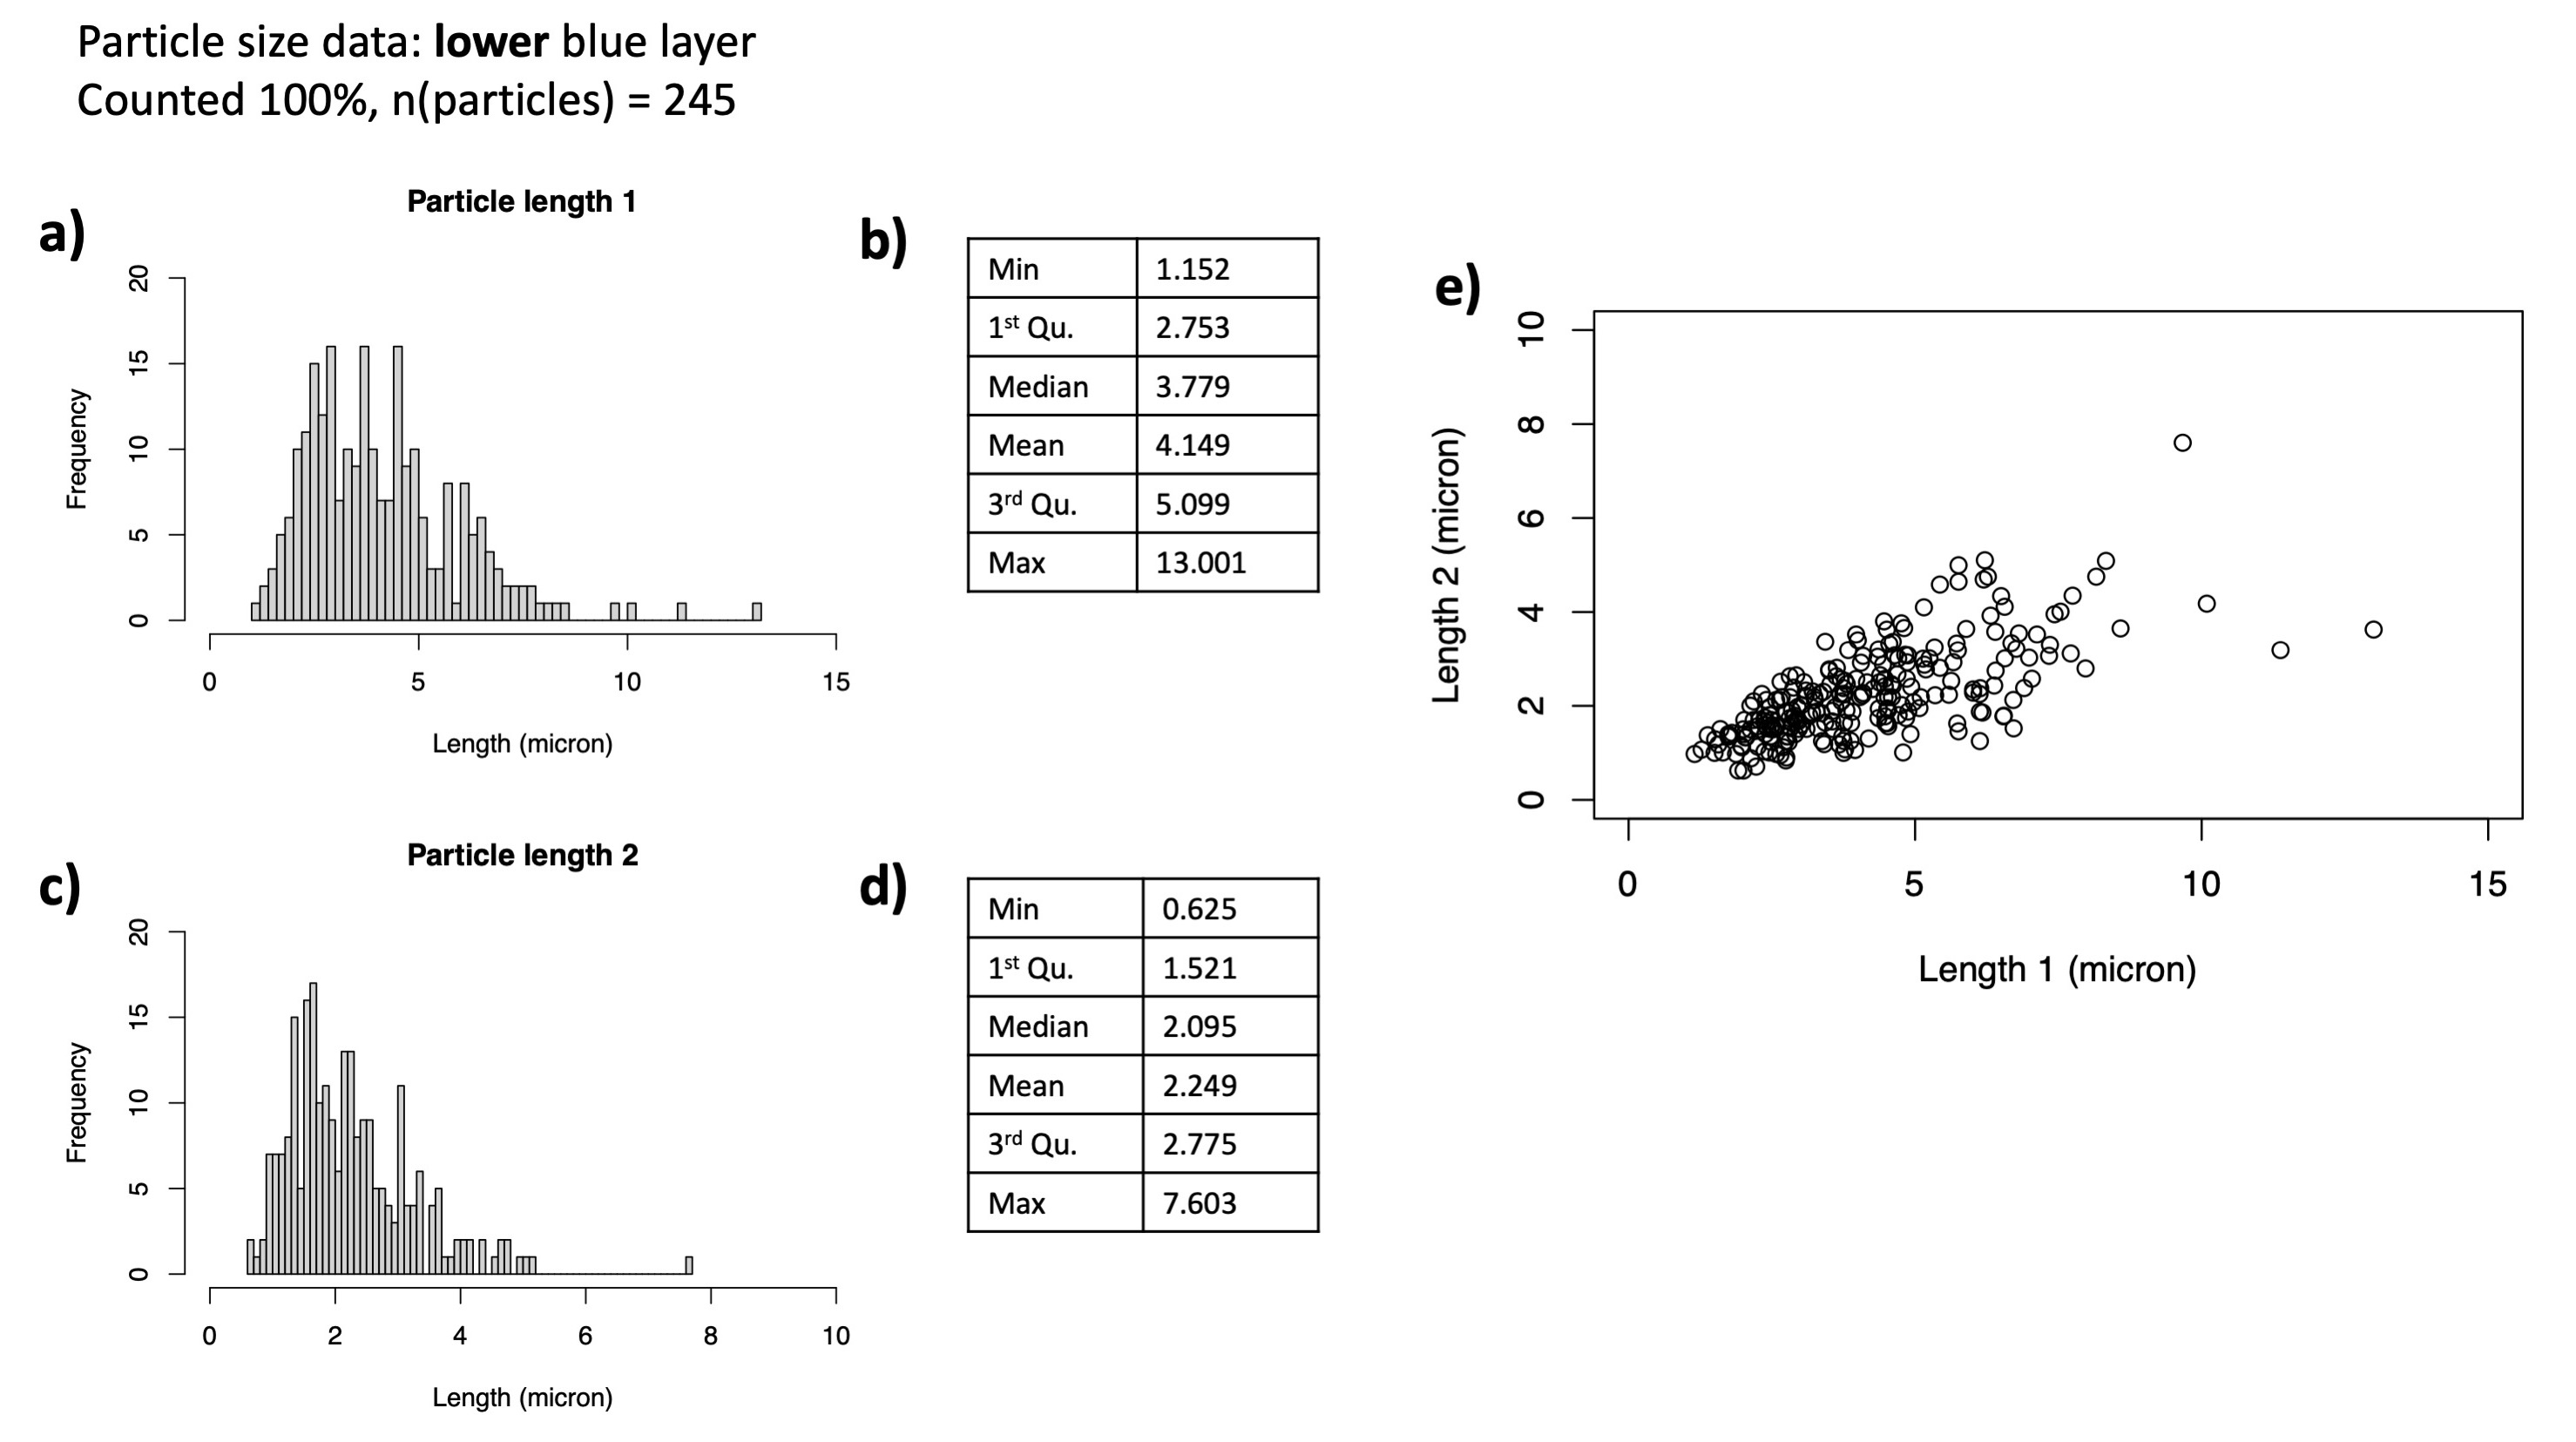
\includegraphics[width=0.8\linewidth]{1259.33_partsize_1}
\caption[Particle size distribution, sample 1259.33, bottom layer.]{Particle size distribution of sample 1259.33, bottom layer: \textbf{a)} Histogram showing distribution of particle length 1 values. \textbf{b)} Descriptive statistics for particle length 1 data. \textbf{c)} Histogram showing distribution of particle length 2 values. \textbf{d)} Descriptive statistics for particle length 2 data. \textbf{e)} Graph of length 1 versus length 2 showing the degree of skew.}
\label{fig:1259.33_partsize_1}
\end{figure}

\begin{figure}[H]
\centering
  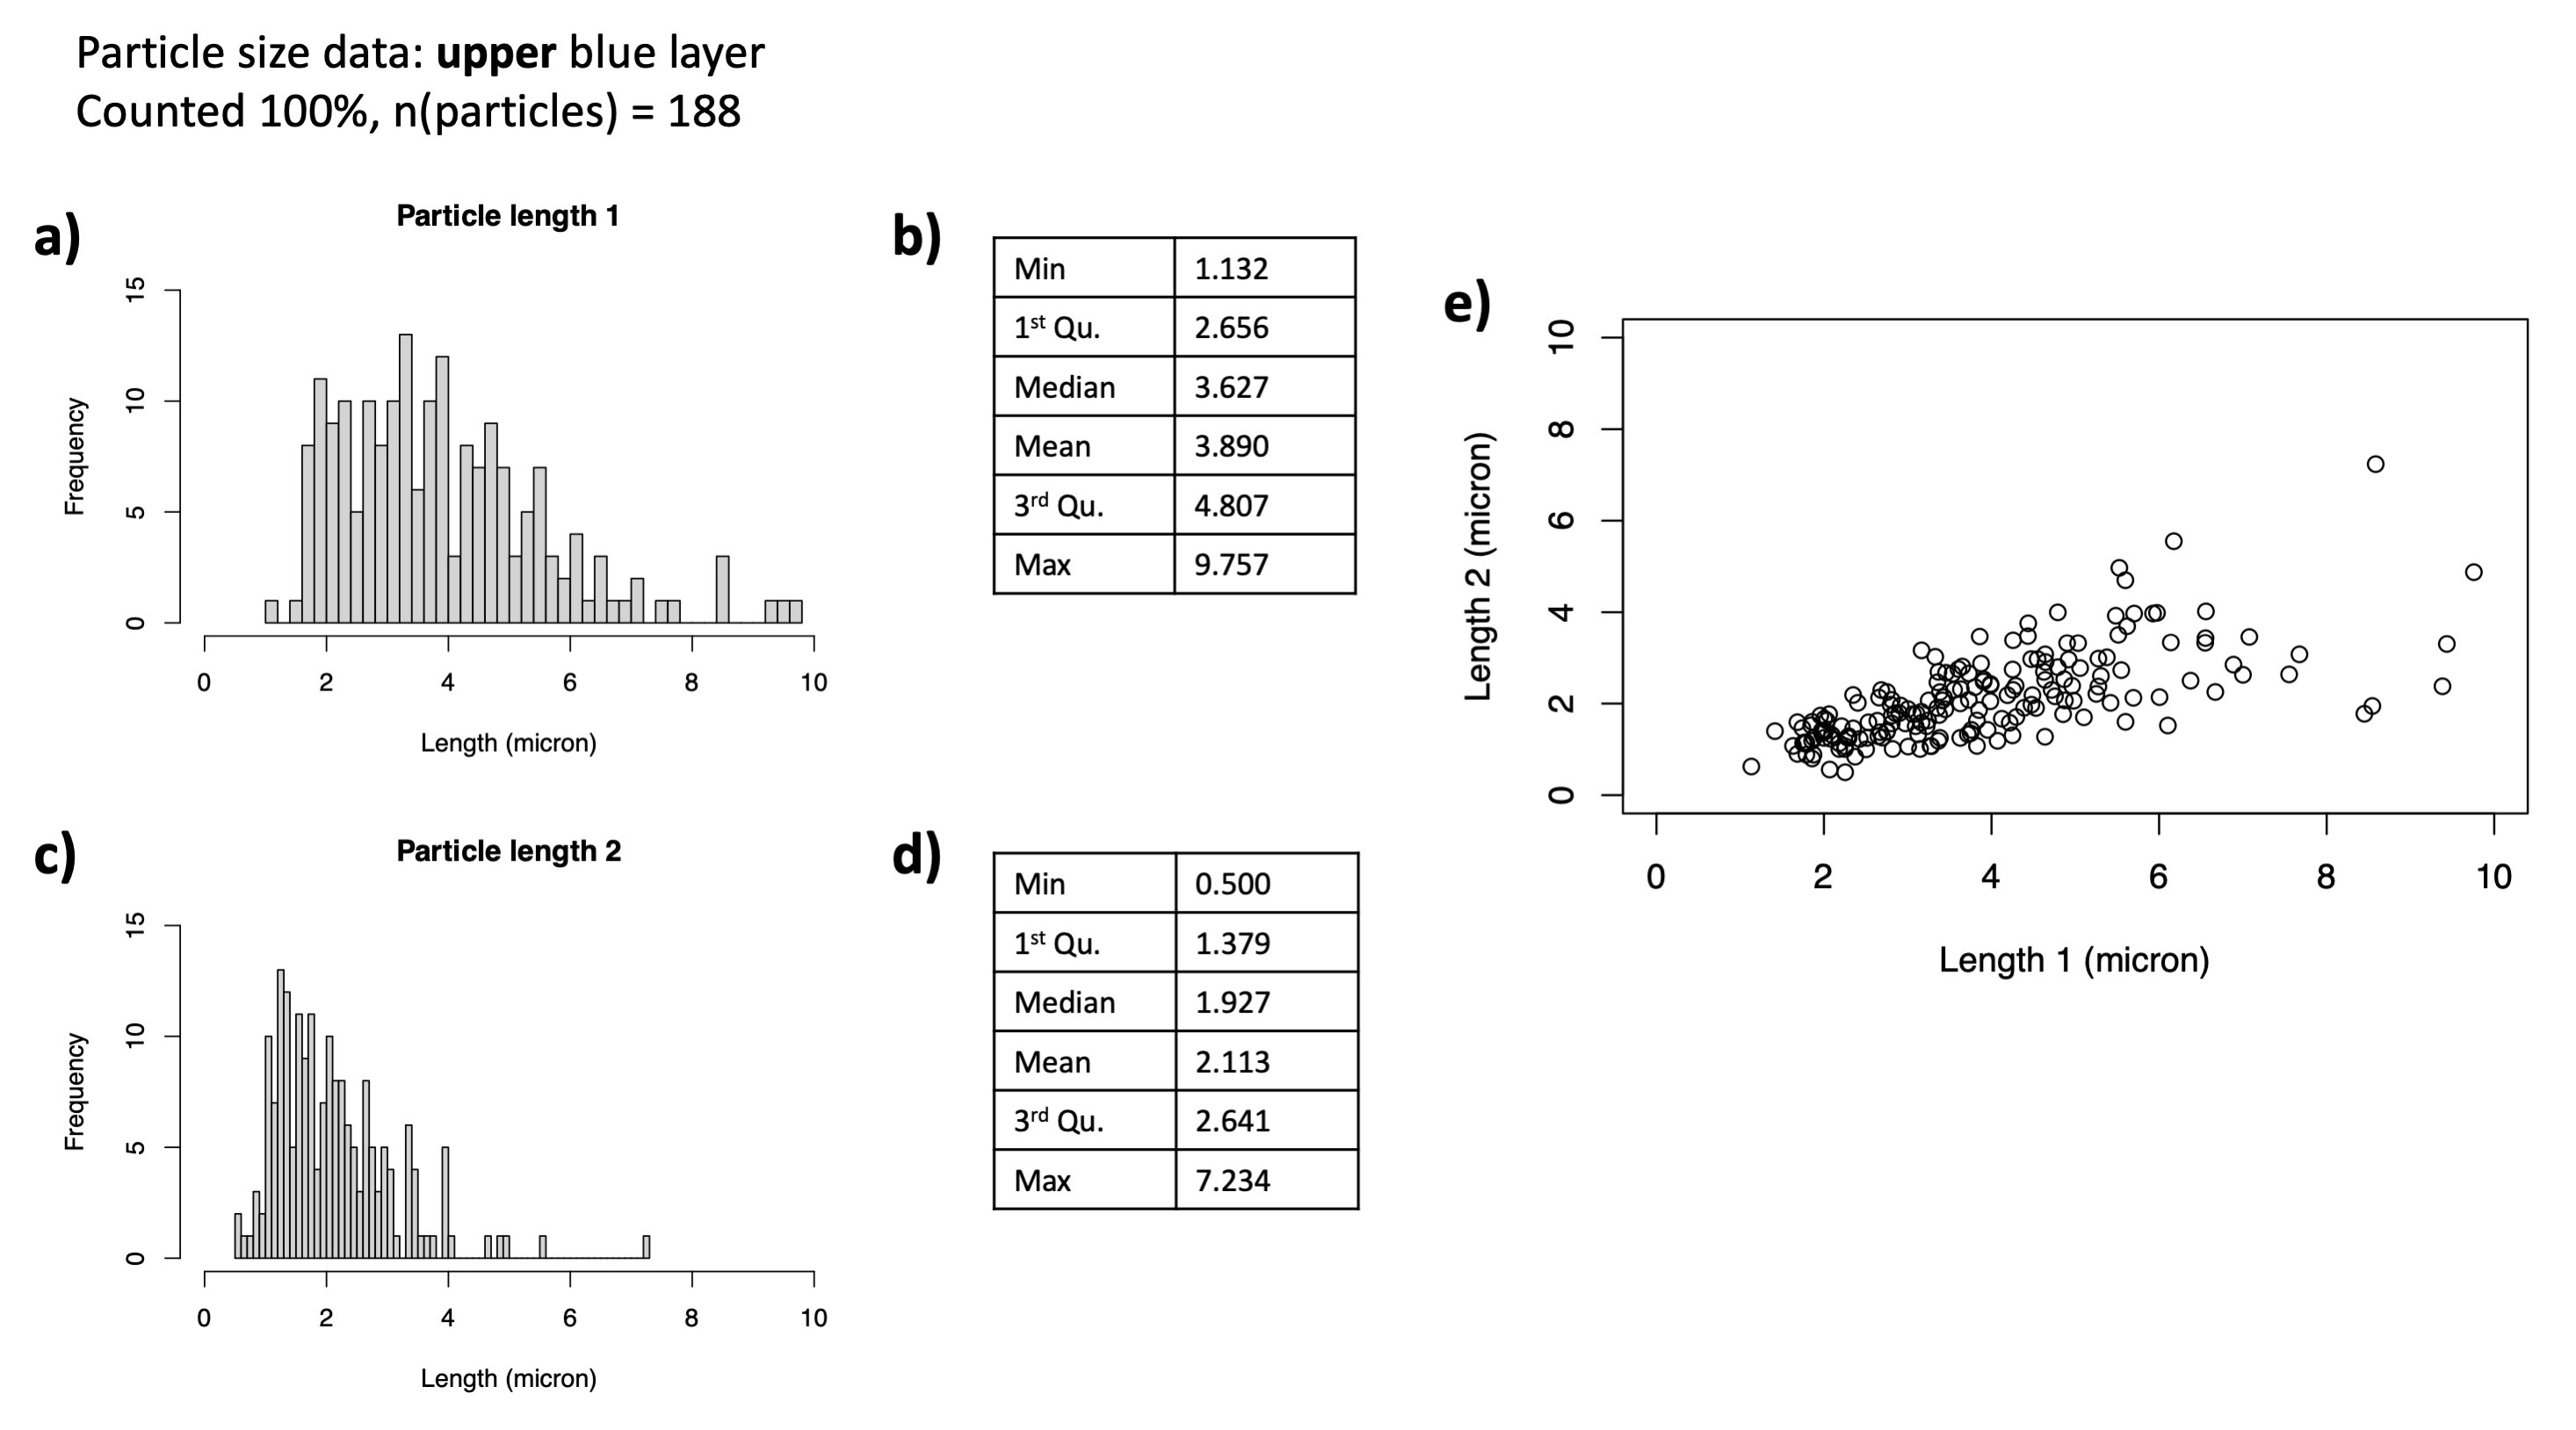
\includegraphics[width=0.8\linewidth]{1259.33_partsize_2}
\caption[Particle size distribution, sample 1259.33, top layer.]{Particle size distribution of sample 1259.33, top layer: \textbf{a)} Histogram showing distribution of particle length 1 values. \textbf{b)} Descriptive statistics for particle length 1 data. \textbf{c)} Histogram showing distribution of particle length 2 values. \textbf{d)} Descriptive statistics for particle length 2 data. \textbf{e)} Graph of length 1 versus length 2 showing the degree of skew.}
\label{fig:1259.33_partsize_2}
\end{figure}


\section{Sample 1259.34}

\textit{Figure \ref{fig:1259.34_imgs}} shows SEM and dark field microscope images of 1259.34, with two distinct original azurite-containing layers. One of these contains a large proportion of white pigment mixed with azurite. EDS mapping (\textit{Figure \ref{fig:1259.34_mapdata}}) shows azurite, iron oxide, aluminosilicates including feldspar, rutile, and dolomite (CaMg(CO\textsubscript{3})\textsubscript{2}). Only the top layer contains lead and arsenic, likely cerussite (lead white).

\textit{Figures \ref{fig:1259.34_partsize_2}} and \textit{\ref{fig:1259.34_partsize_1}} show particle size data for the bottom and top layers containing azurite. These layers do not differ except a small number of outlying large particles in the bottom layer, and both contain small pigments with approximate average dimensions length 1 = 2(length2). 

\begin{figure}[H]
  \centering
  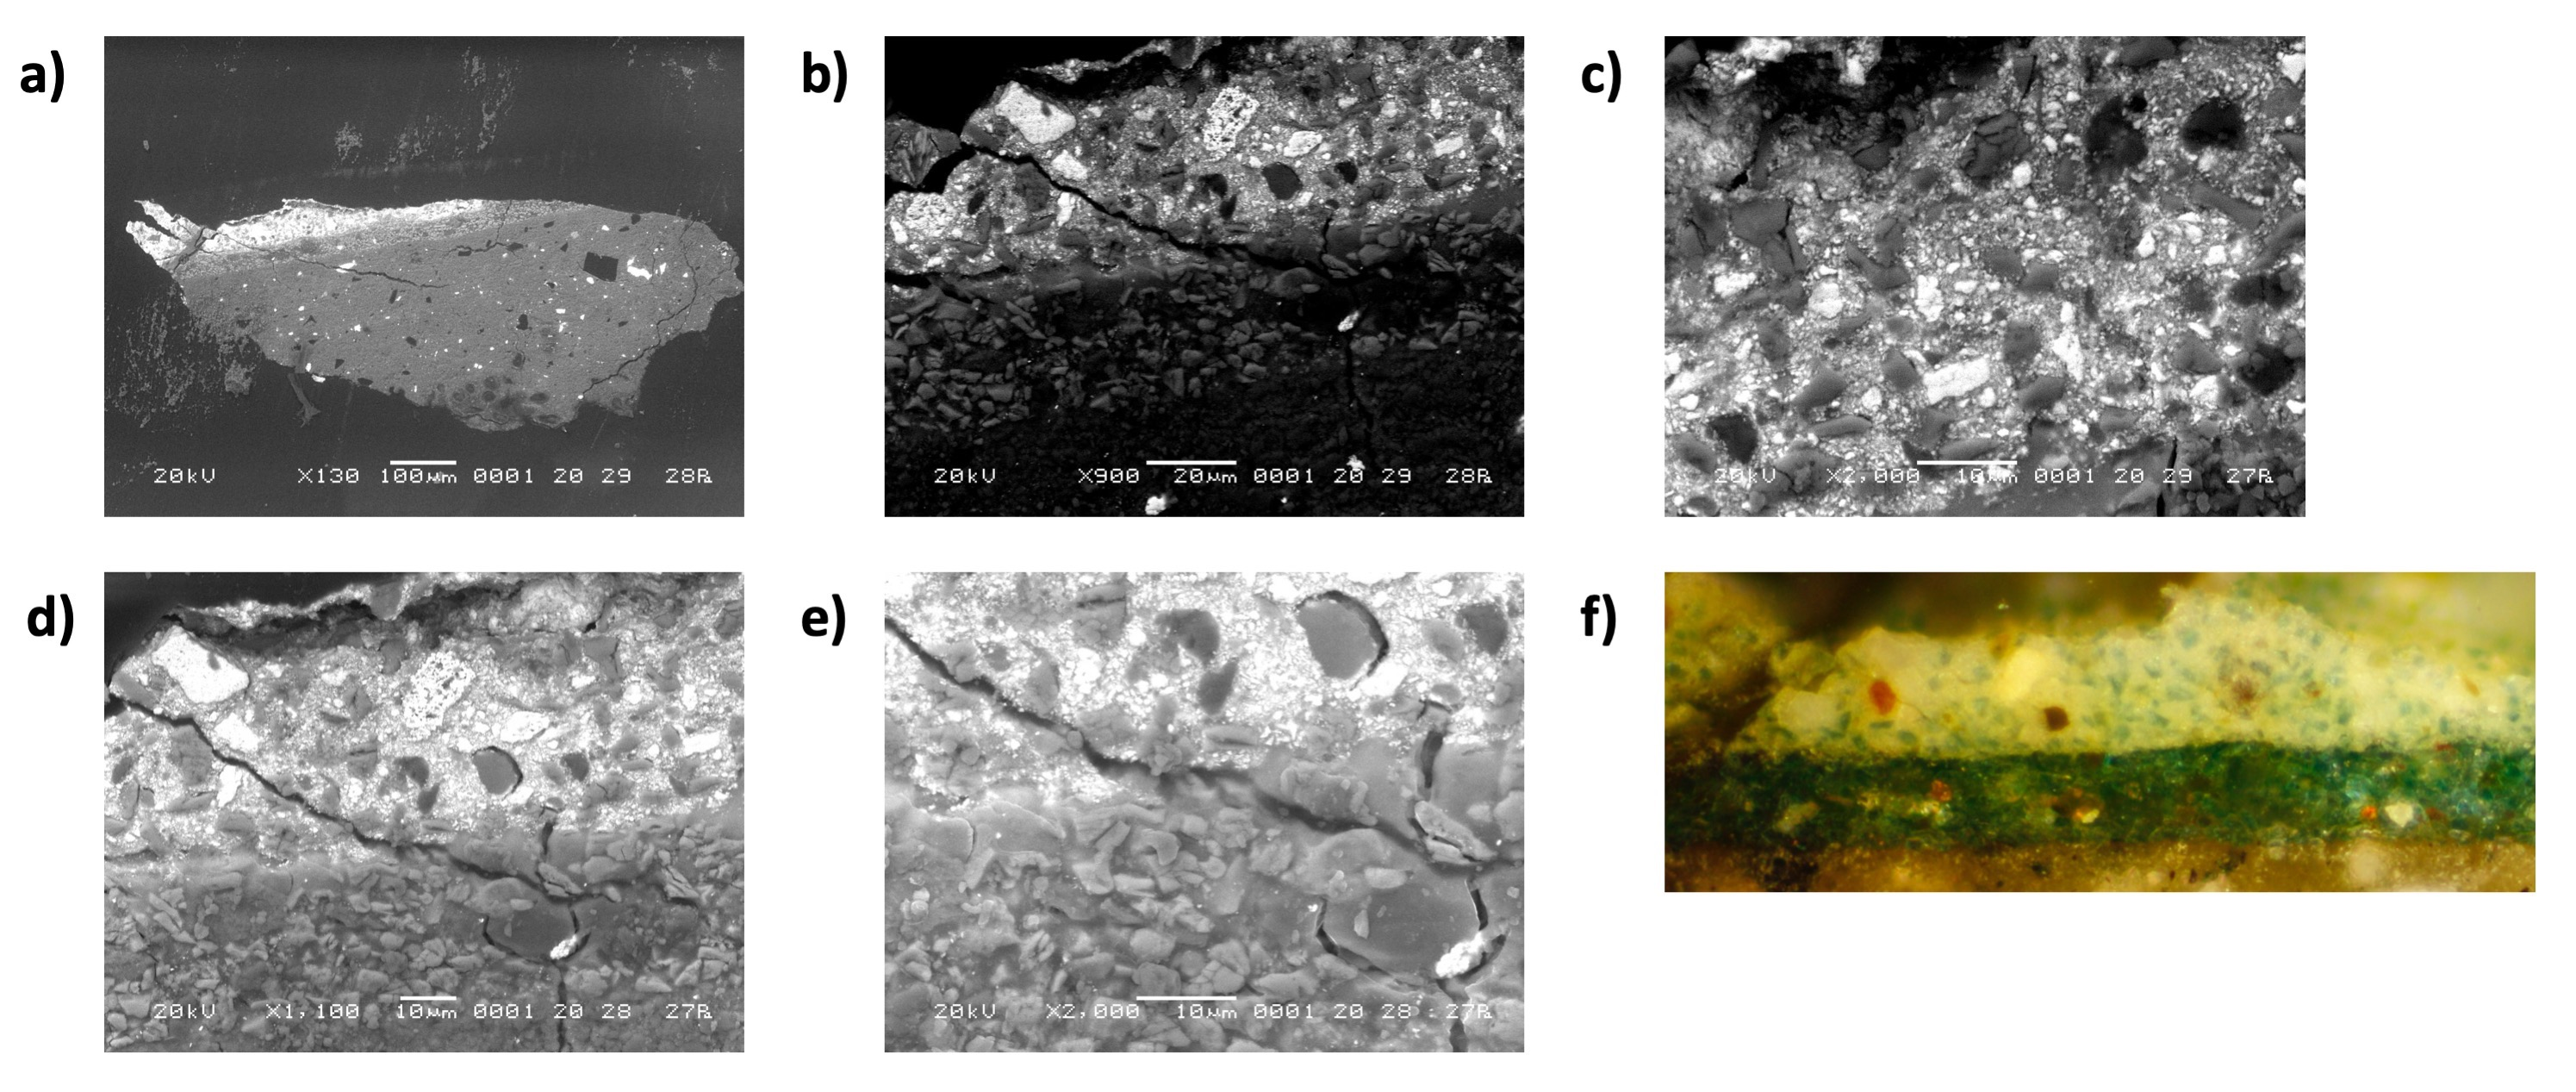
\includegraphics[width=0.8\linewidth]{1259.34_imgs}
\caption[SEM and dark field images of sample 1259.34.]{SEM and dark field images of sample 1259.34: \textbf{a)} 130x magnification showing two distinct layers containing azurite (both original), \textbf{b)} 900x magnification, \textbf{c)} 2000x magnification, \textbf{d)} 1100x magnification, \textbf{e)} 2000x magnification, \textbf{f)} dark field microscope image showing two distinct layers. Dark field microscope images courtesy of Katharine Waldron, HKI.}
\label{fig:1259.34_imgs}
\end{figure}

\begin{figure}[H]
\centering
\begin{minipage}[t]{\linewidth}
  \centering
  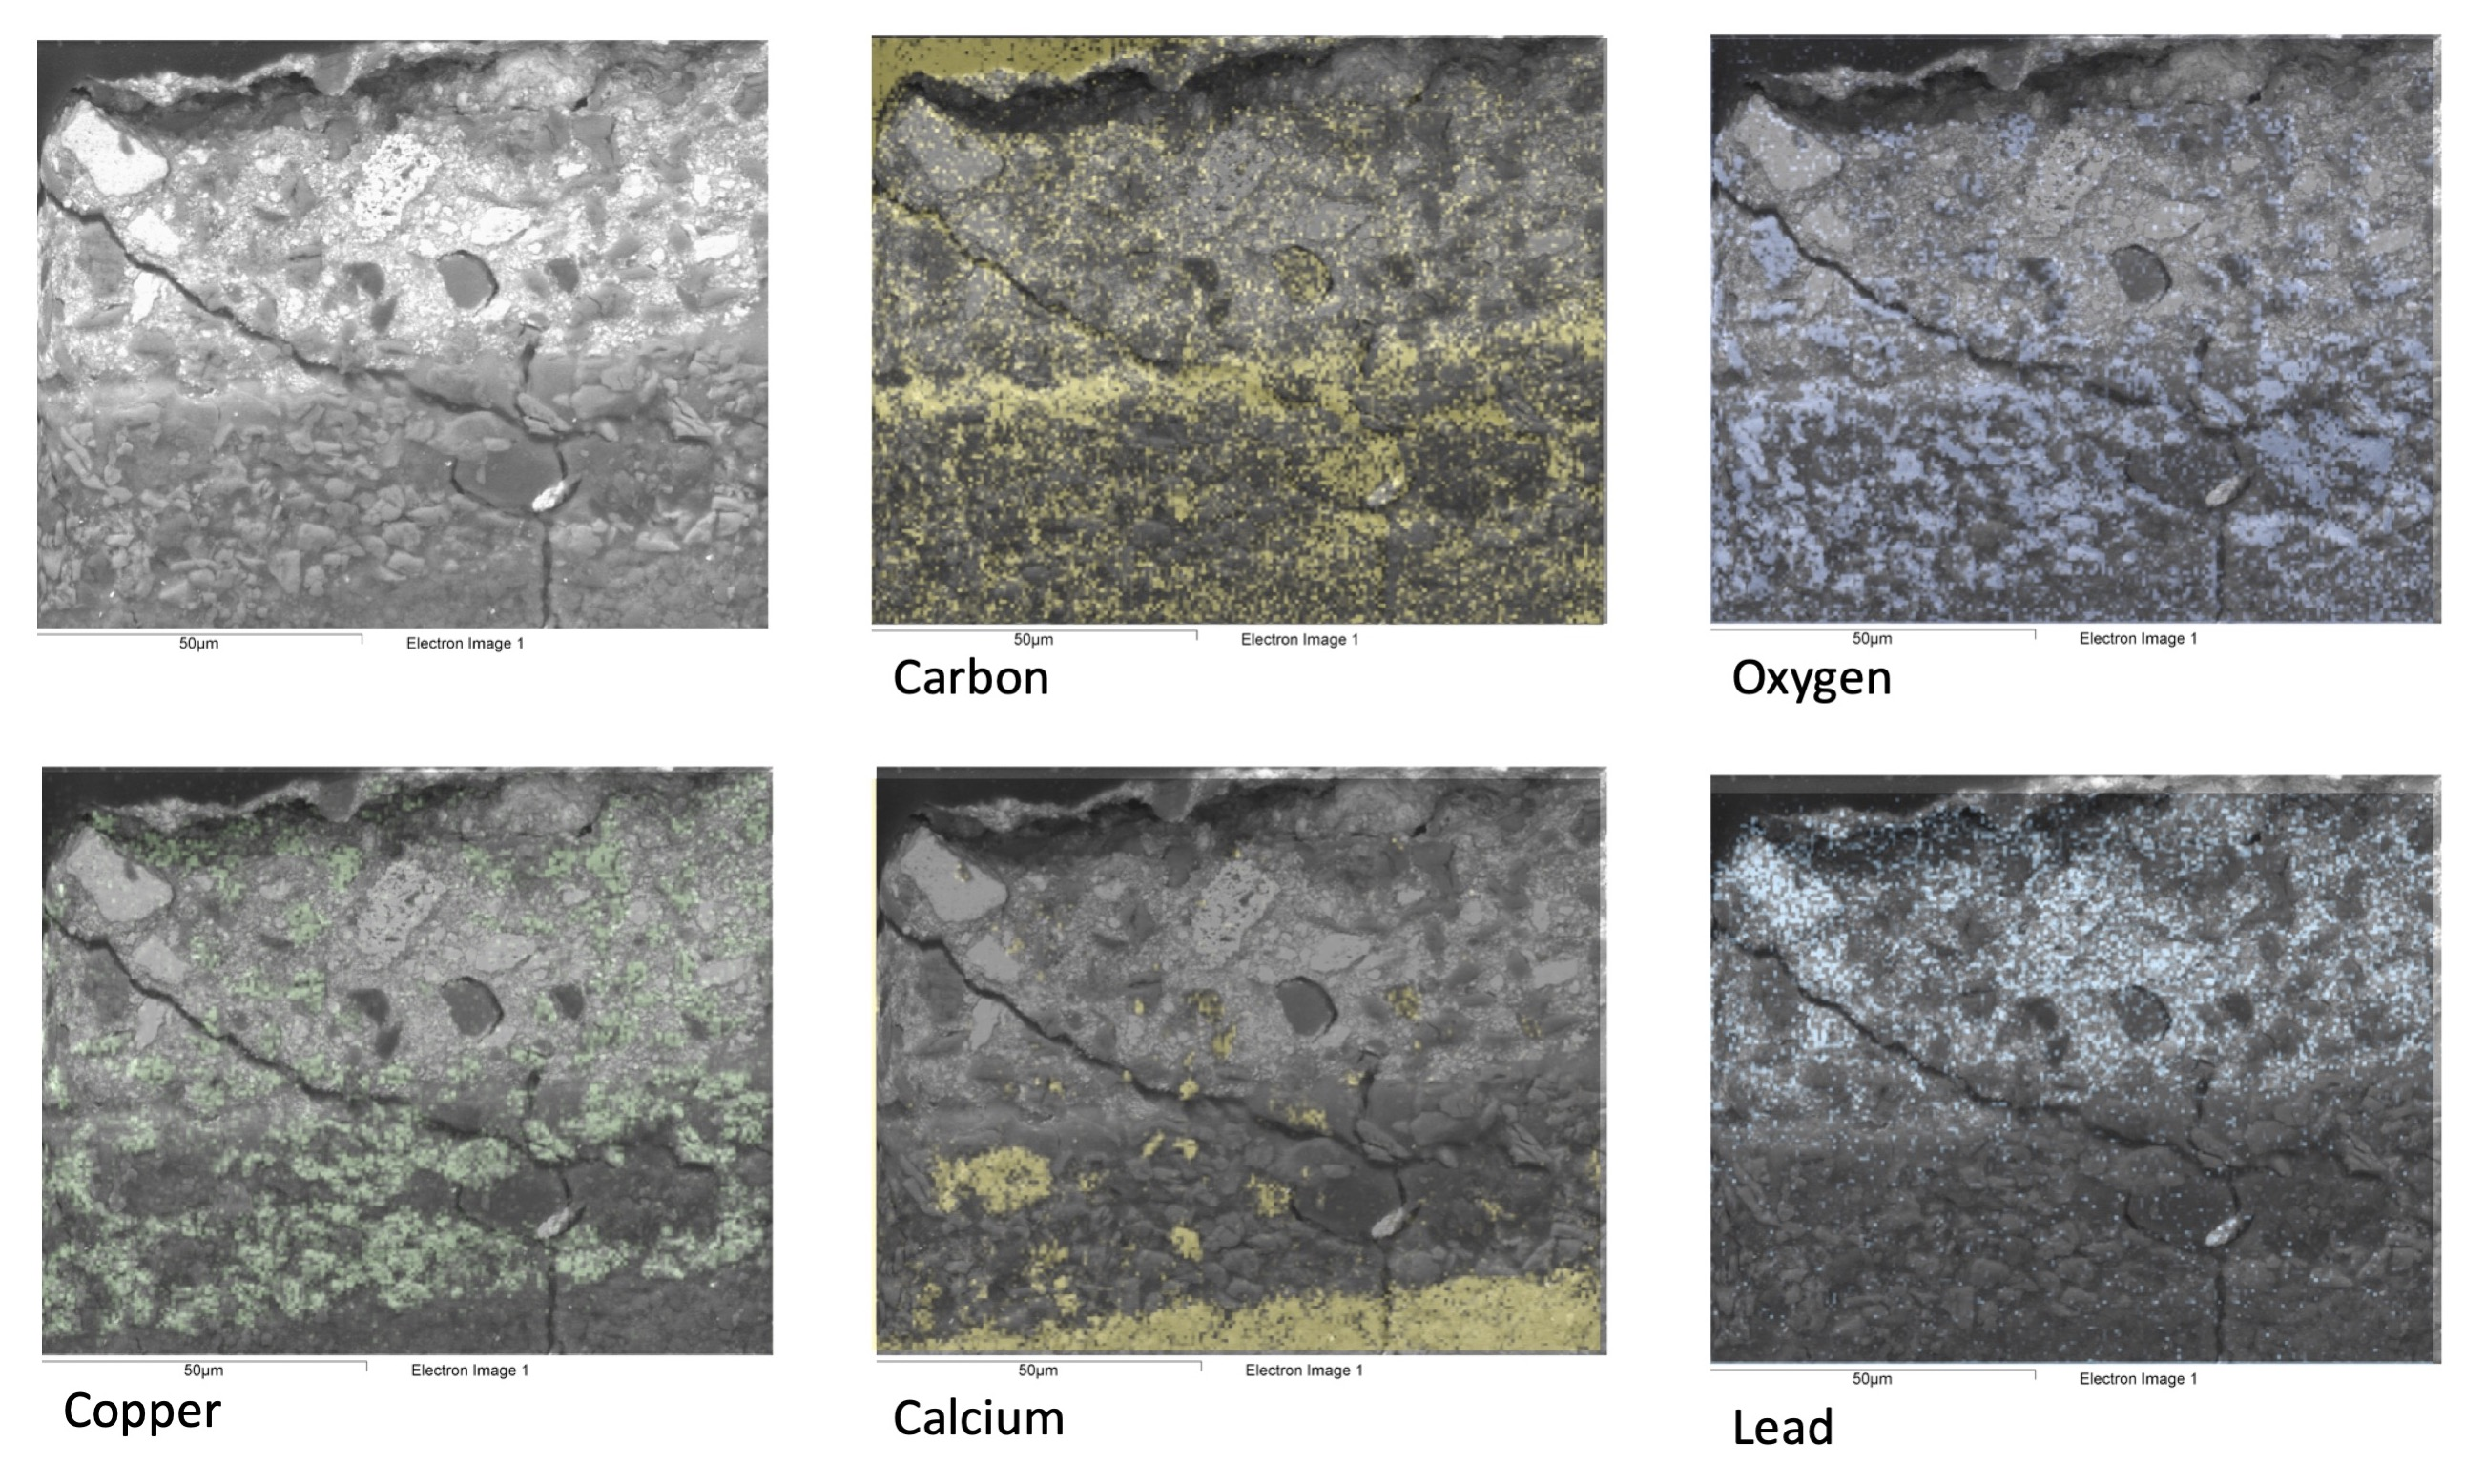
\includegraphics[width=0.9\linewidth]{1259.34_mapdata_1}
\hfill
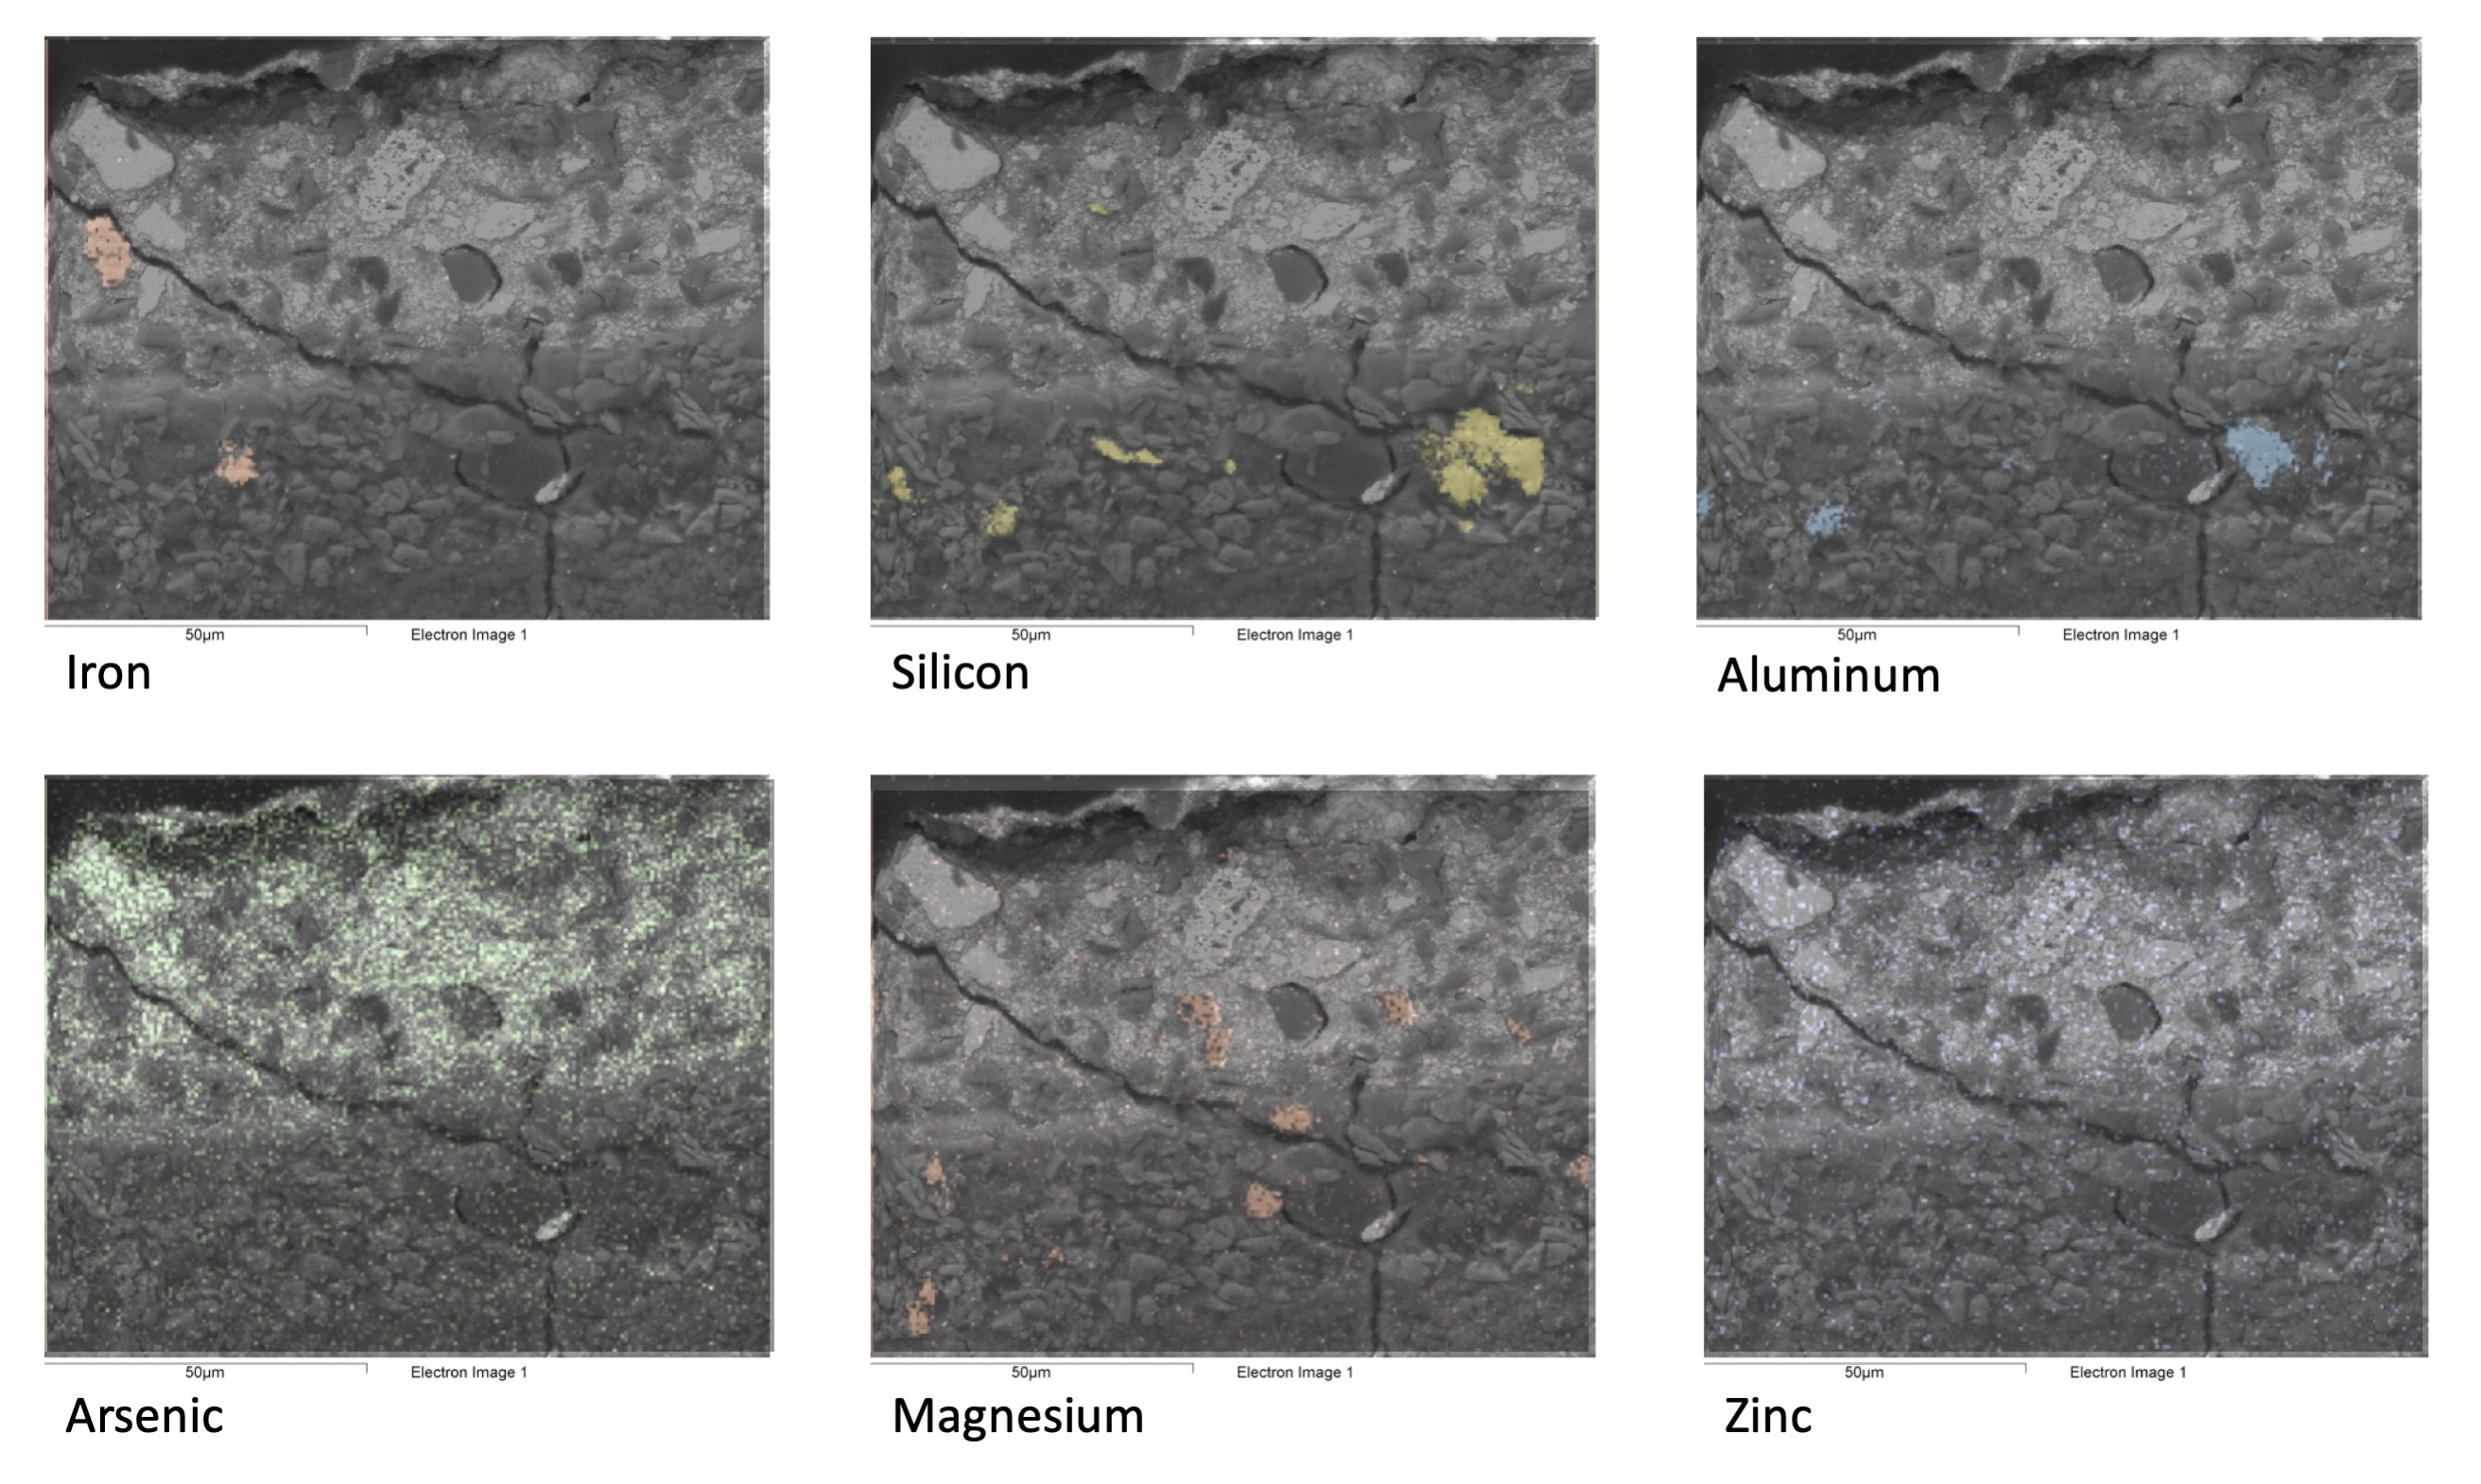
\includegraphics[width=0.9\linewidth]{1259.34_mapdata_2}
\hfill
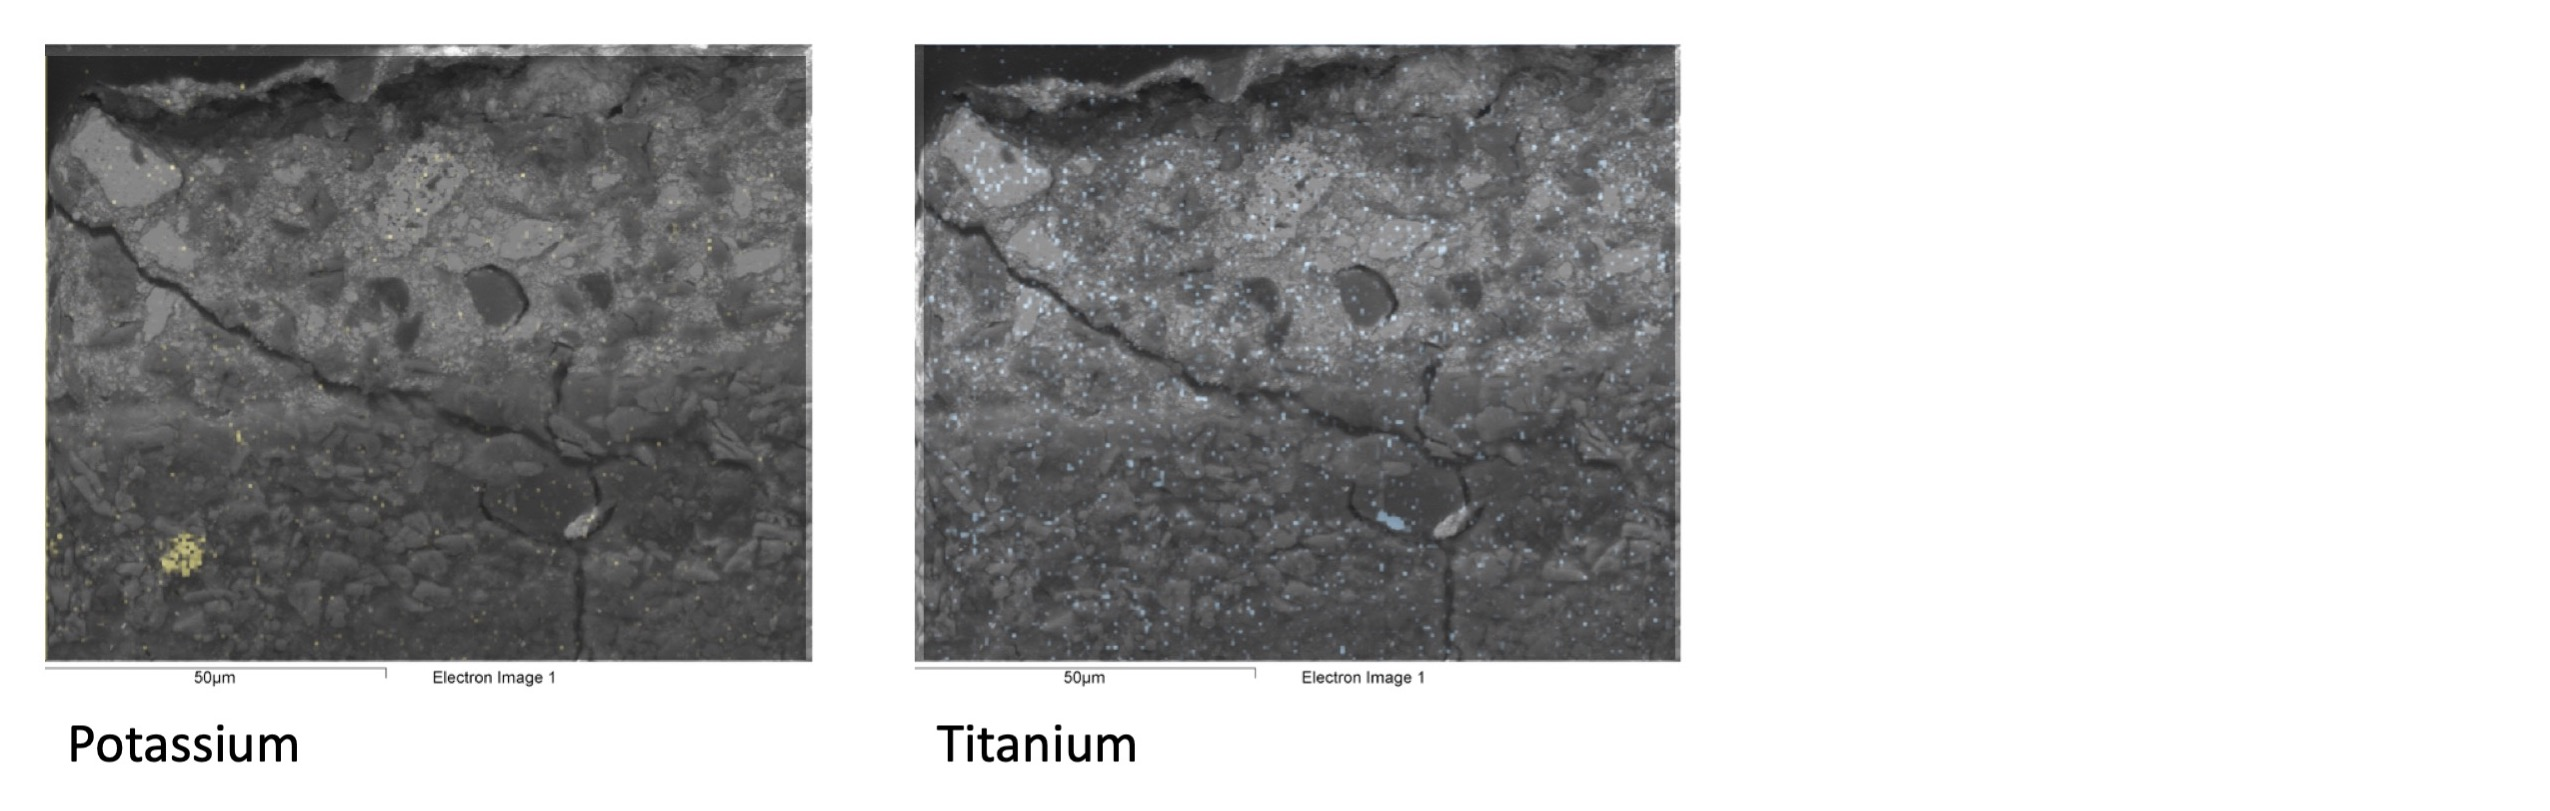
\includegraphics[width=0.9\linewidth]{1259.34_mapdata_3}
\hfill
\end{minipage}
\caption[EDS map data, sample 1259.34.]{EDS map data of sample 1259.34 showing locations of elements in both azurite-containing layers. Elements detected are C, O, Ca, Cu, K, Ti, Zn, P, Fe, Mg, and Pb.}C, O, Cu, Ca, Pb, Fe, Si, Al, As, Mg, Zn, K, Ti.}
\label{fig:1259.34_mapdata}
\end{figure}

\begin{figure}[H]
\centering
  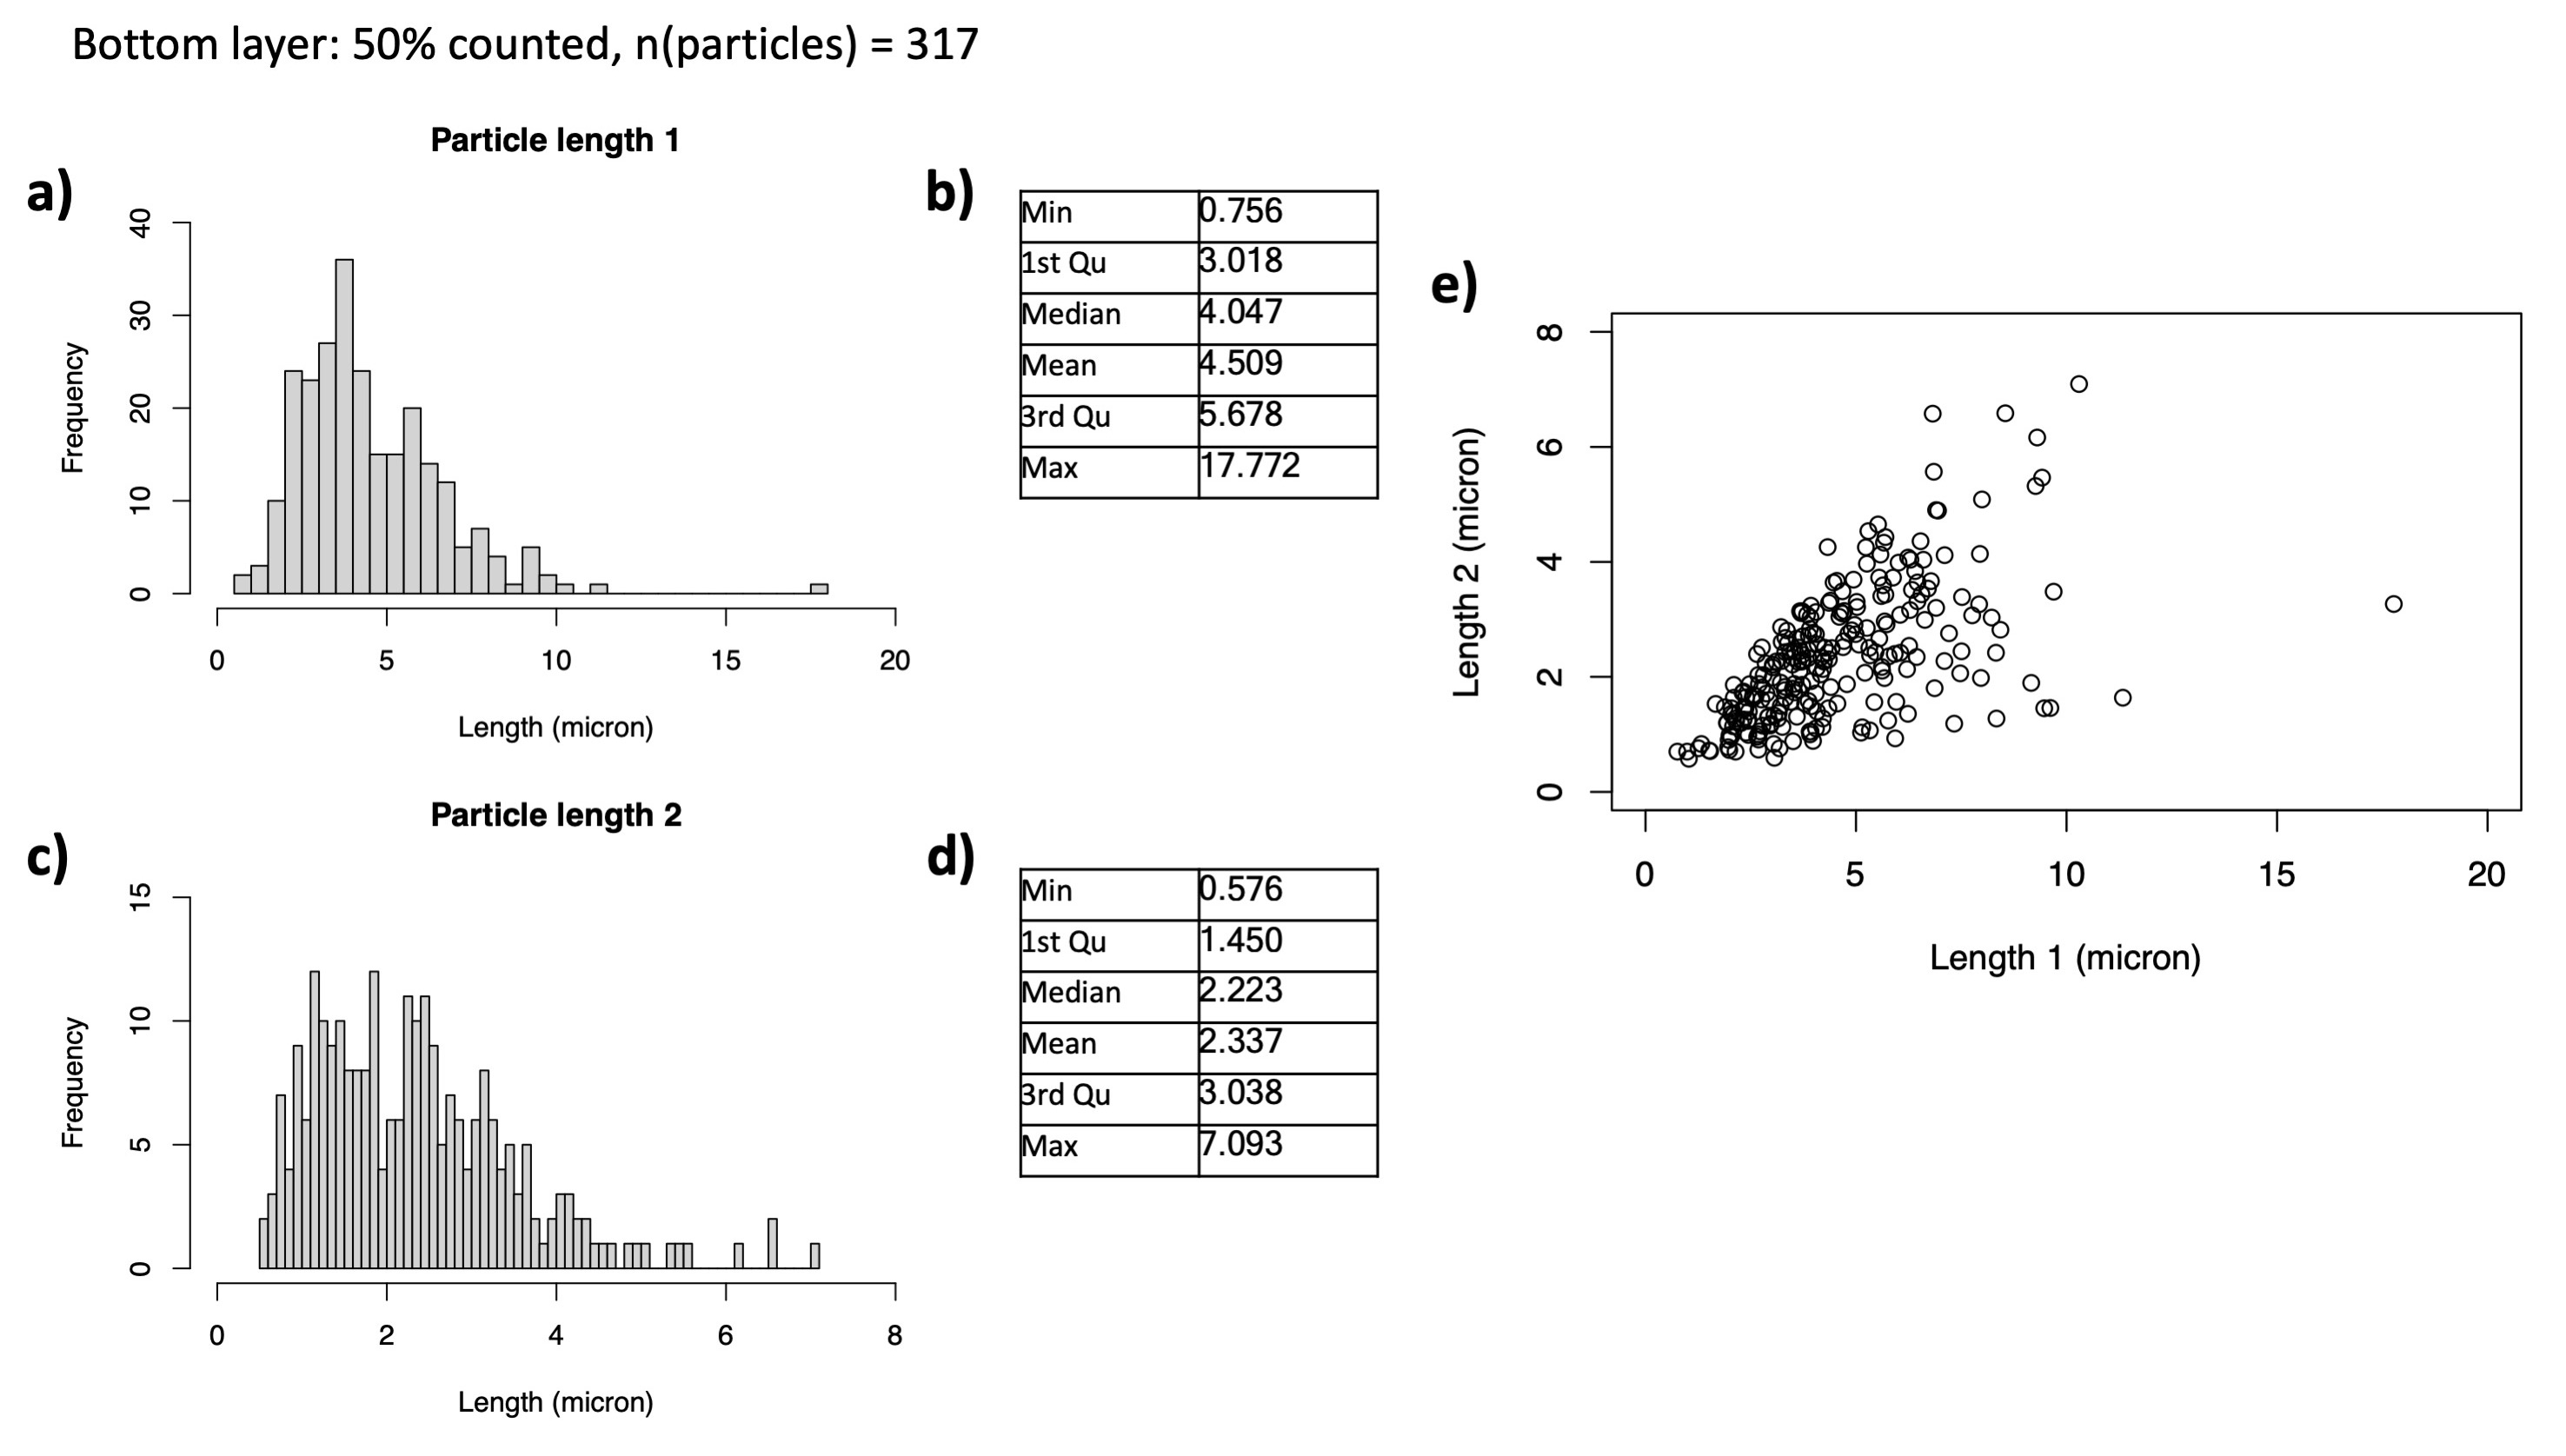
\includegraphics[width=0.8\linewidth]{1259.34_partsize_2}
\caption[Particle size distribution, sample 1259.34, bottom layer.]{Particle size distribution of sample 1259.34, bottom layer: \textbf{a)} Histogram showing distribution of particle length 1 values. \textbf{b)} Descriptive statistics for particle length 1 data. \textbf{c)} Histogram showing distribution of particle length 2 values. \textbf{d)} Descriptive statistics for particle length 2 data. \textbf{e)} Graph of length 1 versus length 2 showing the degree of skew.}
\label{fig:1259.34_partsize_2}
\end{figure}

\begin{figure}[H]
\centering
  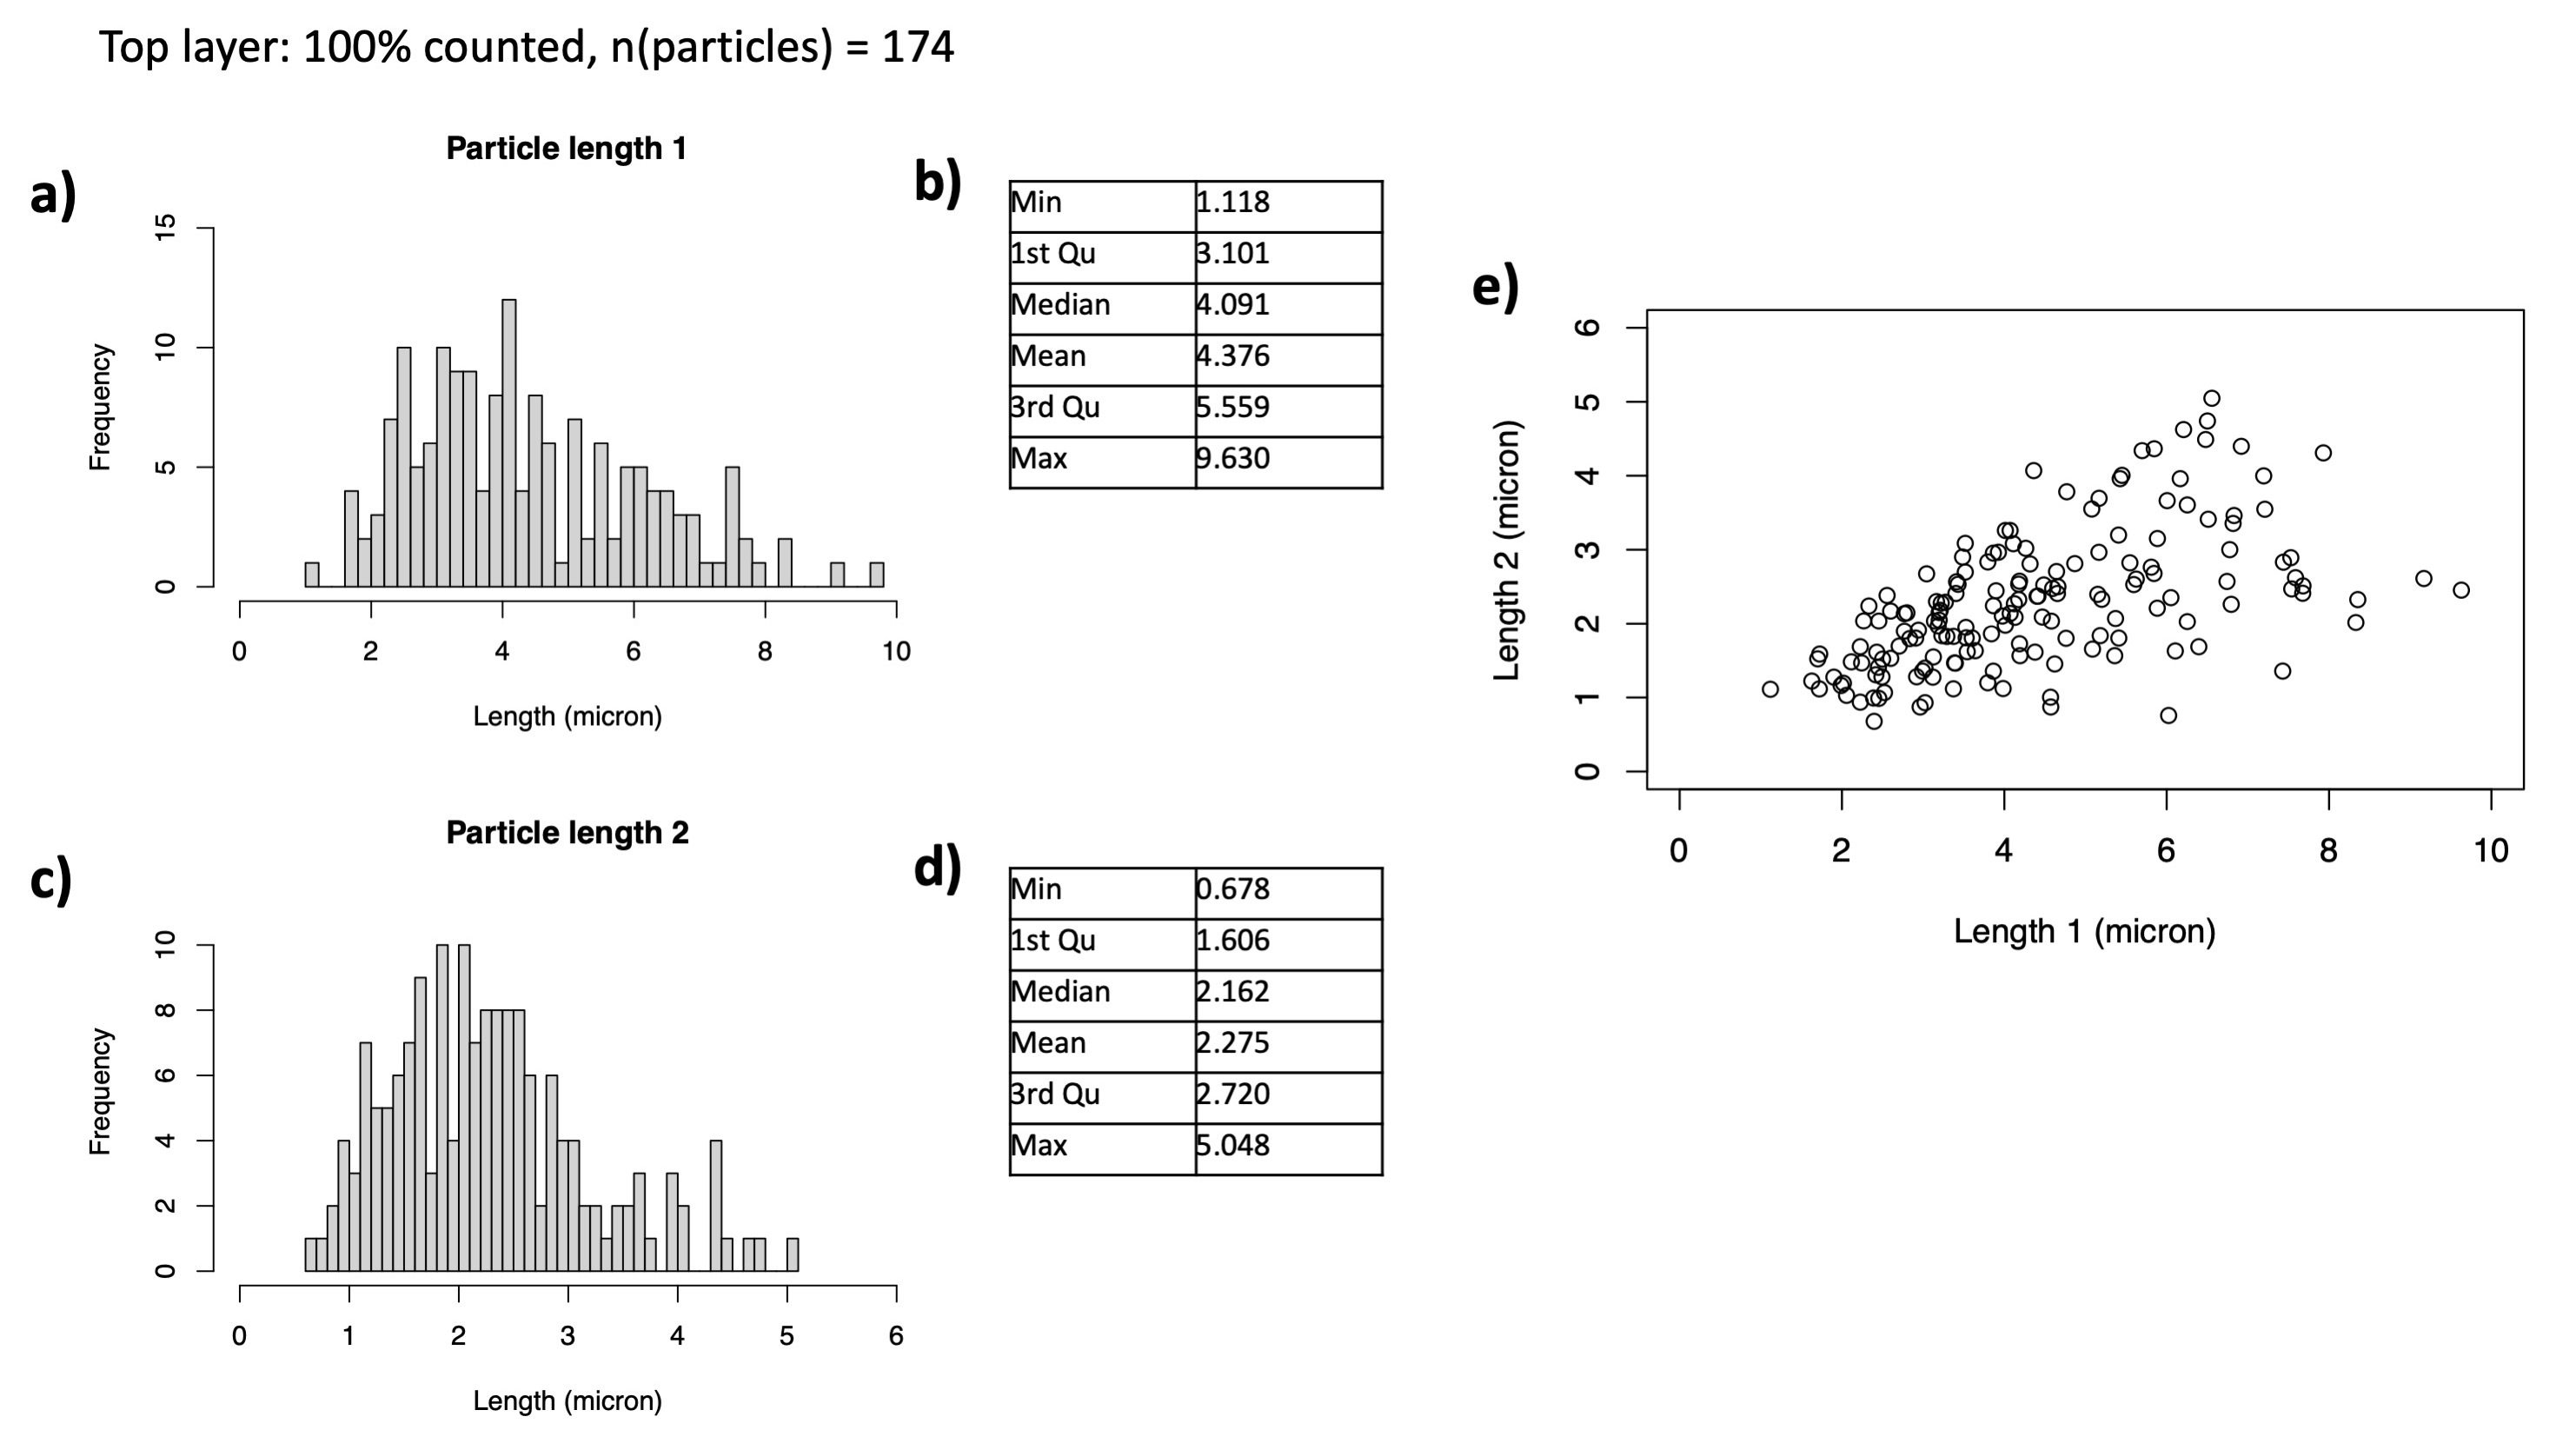
\includegraphics[width=0.8\linewidth]{1259.34_partsize}
\caption[Particle size distribution, sample 1259.34, top layer.]{Particle size distribution of sample 1259.34, top layer: \textbf{a)} Histogram showing distribution of particle length 1 values. \textbf{b)} Descriptive statistics for particle length 1 data. \textbf{c)} Histogram showing distribution of particle length 2 values. \textbf{d)} Descriptive statistics for particle length 2 data. \textbf{e)} Graph of length 1 versus length 2 showing the degree of skew.}
\label{fig:1259.34_partsize_1}
\end{figure}


\section{Sample 1259.49}

\textit{Figures \ref{fig:1259.49_imgs}-\ref{fig:1259.49_partsize}} show SEM and dark field microscope images, EDS maps, and particle size statistics for 1259.49. Imaging of the sample suggests relatively impure azurite pigments, with many inclusions. Mapping data shows azurite as well as aluminosilicates, a small number of iron-based particles, a titanium compound that is likely rutile, and a compound containing lead, sulfur, and arsenic, likely galena. Statistical analysis of particle size/shape shows small particles that are fairly uniform (few outliers) and round rather than skewed.

\begin{figure}[H]
  \centering
  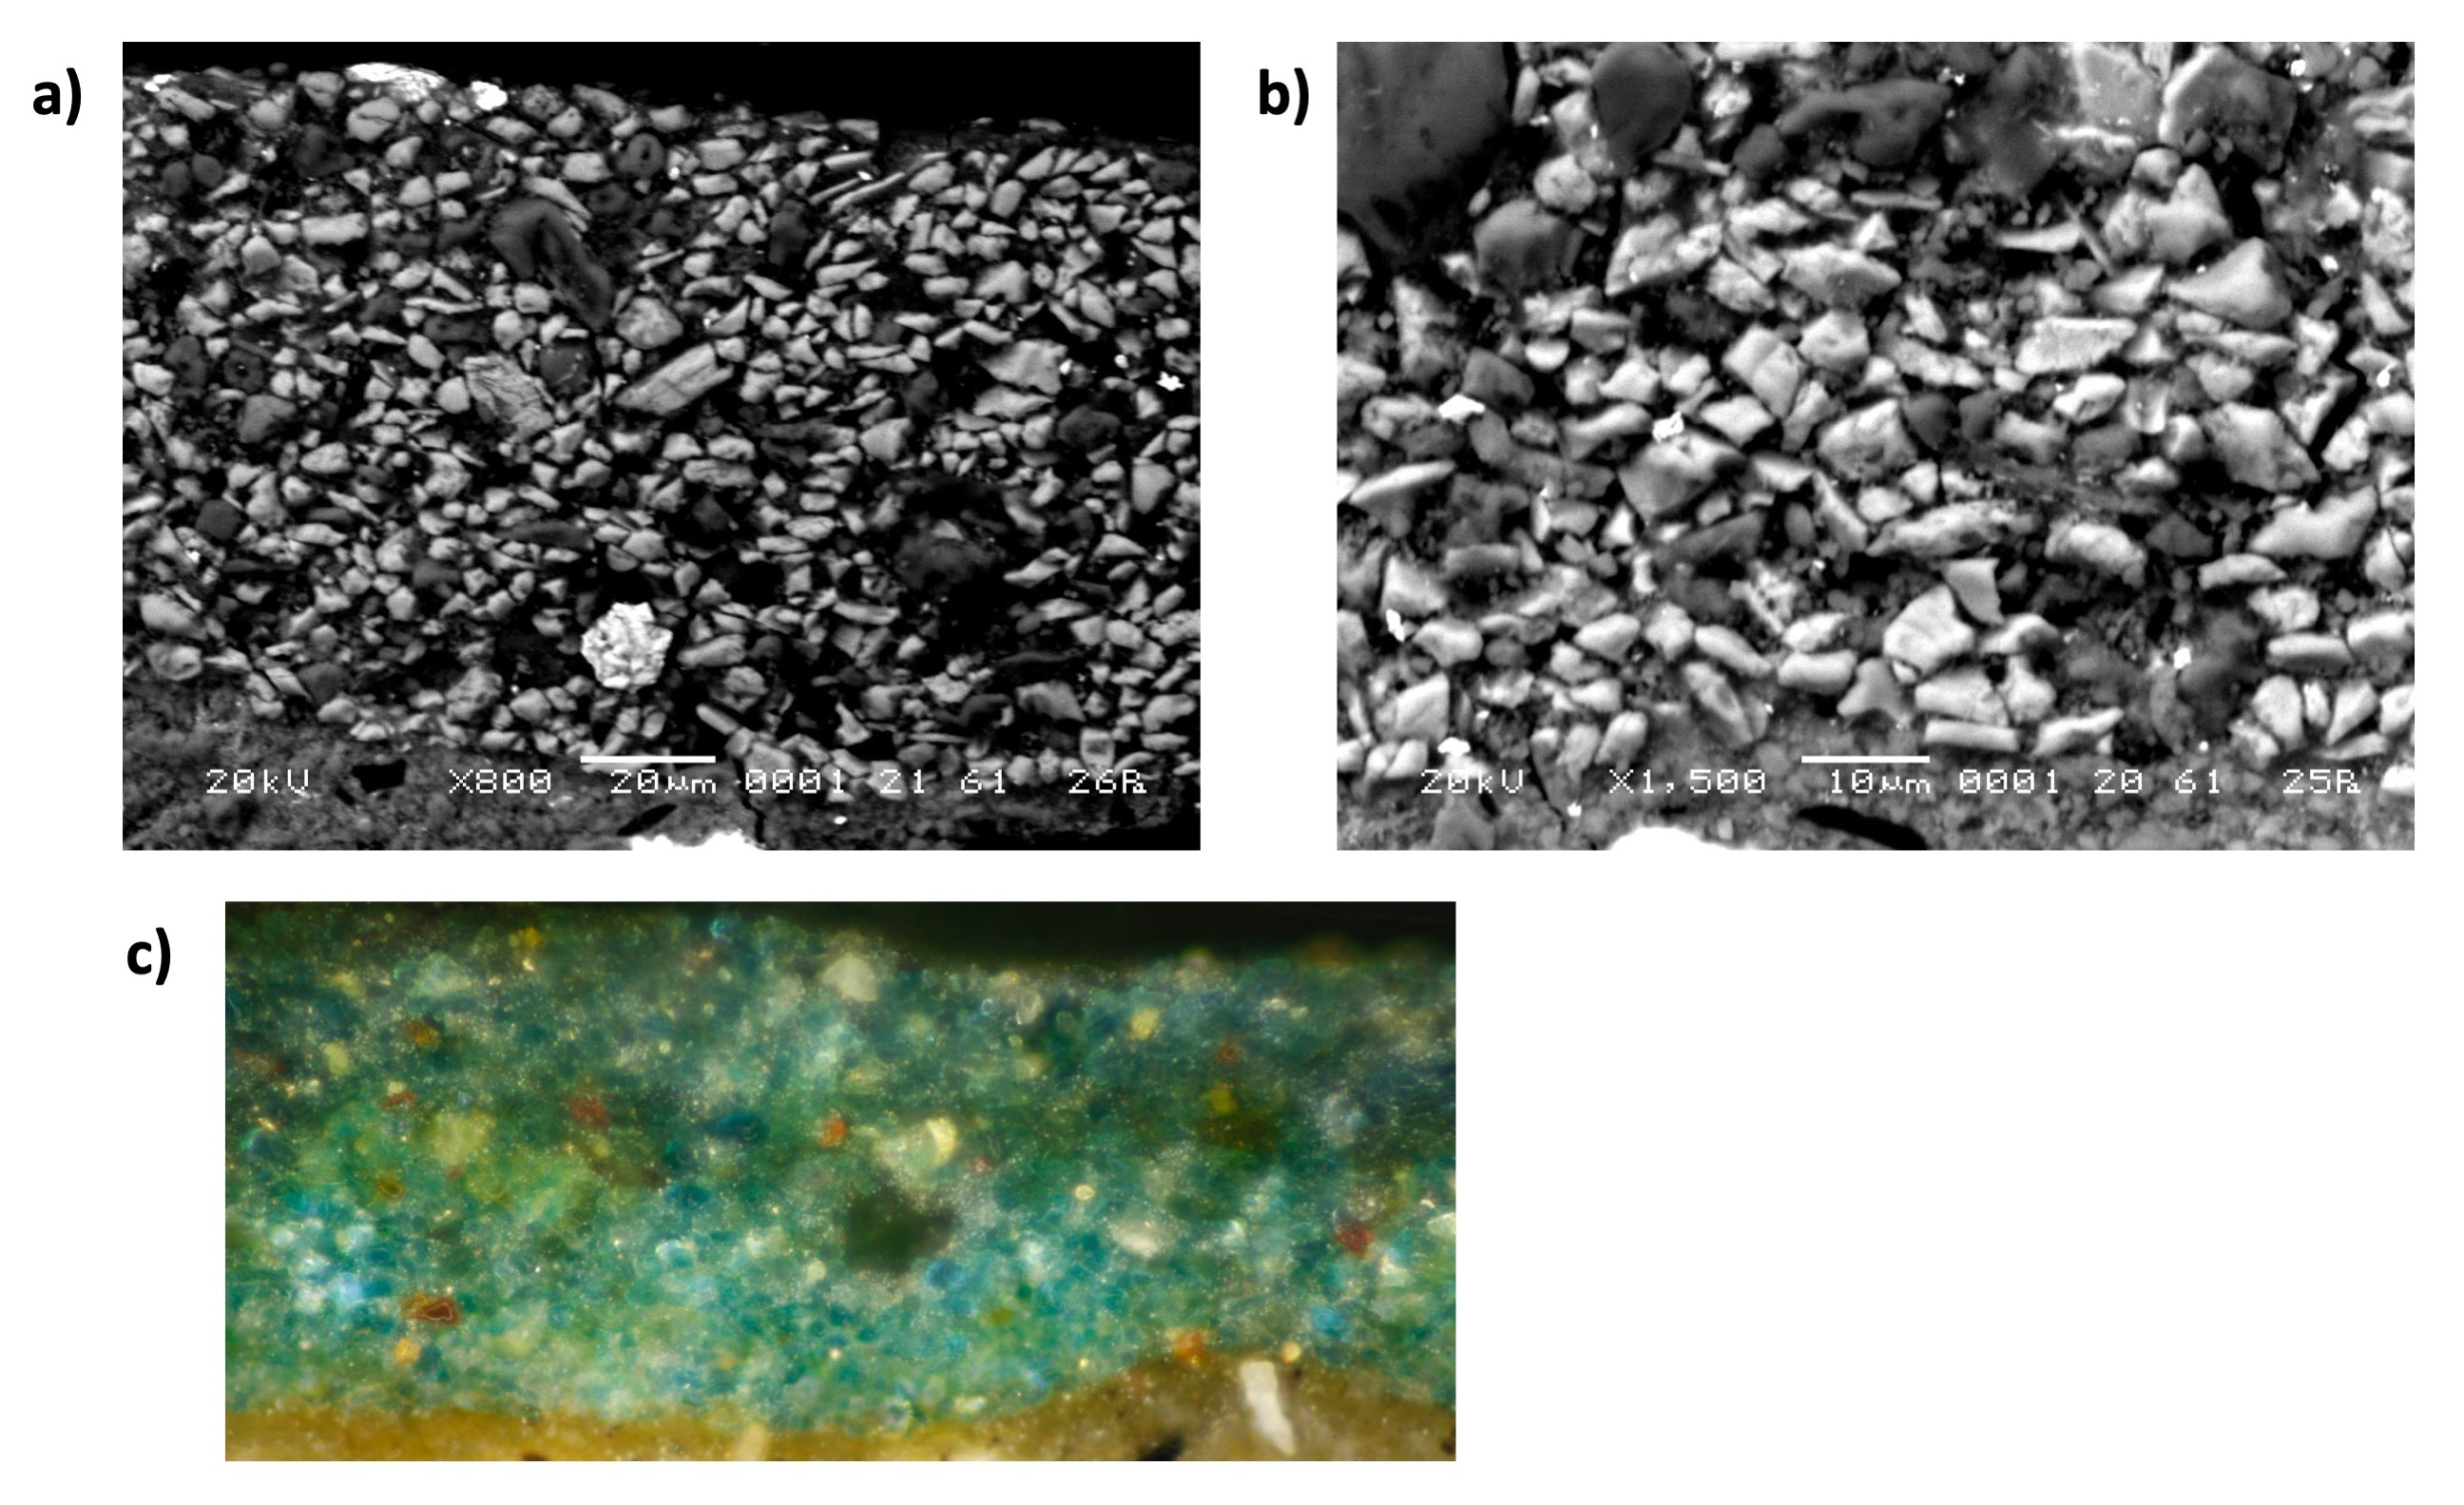
\includegraphics[width=0.8\linewidth]{1259.49_imgs}
\caption[SEM and dark field microscope images of sample 1259.49.]{SEM and dark field microscope images of sample 1259.49: \textbf{a)} 800x magnification, \textbf{b)} 1500x magnification, \textbf{c)} dark field microscope image of sample. Dark field microscope images courtesy of Katharine Waldron, HKI.}
\label{fig:1259.49_imgs}
\end{figure}

\begin{figure}[H]
\centering
\begin{minipage}[t]{\linewidth}
  \centering
  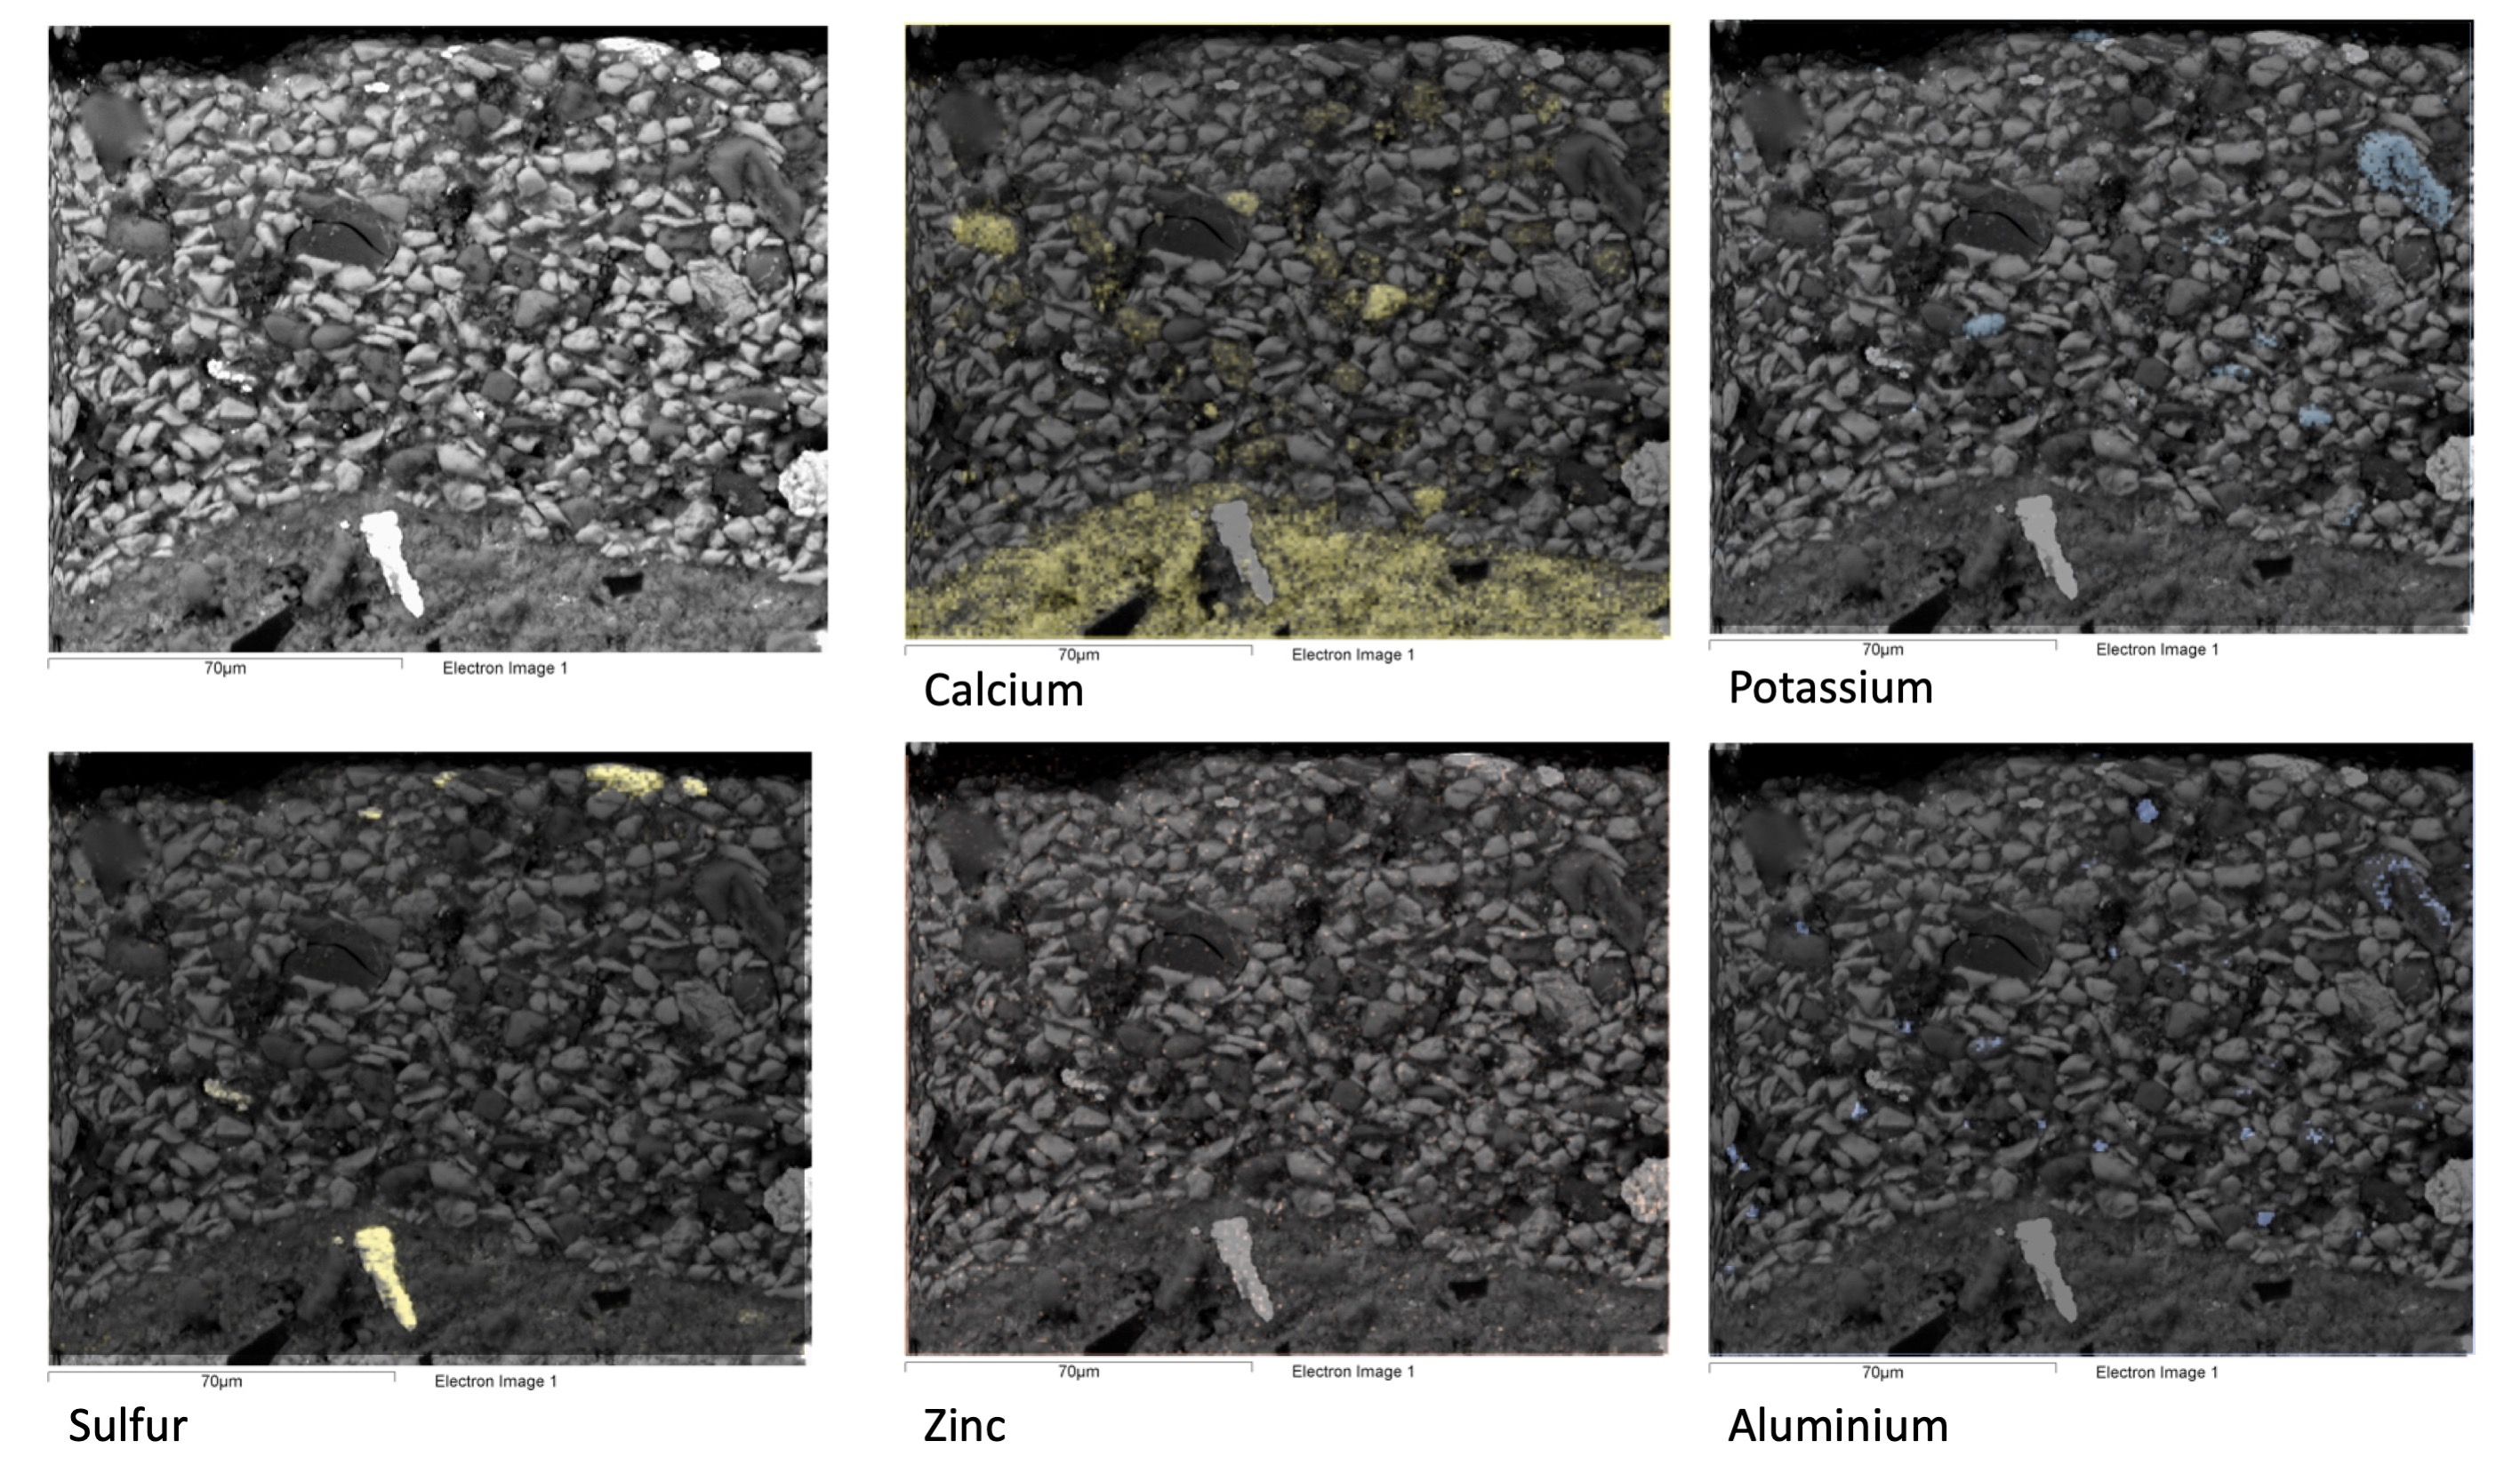
\includegraphics[width=0.9\linewidth]{1259.49_mapdata_1}
\hfill
\includegraphics[width=0.9\linewidth]{1259.49_mapdata_2}
\hfill
\includegraphics[width=0.9\linewidth]{1259.49_mapdata_3}
\hfill
\end{minipage}
\caption[EDS map data, sample 1259.49.]{EDS map data of sample 1259.49 showing locations of elements in an area of the azurite paint layer. Elements detected are Ca, K, S, Zn, Al, Cu, Fe, Ti, Pb, As, Si, and P.}
\label{fig:1259.49_mapdata}
\end{figure}


\begin{figure}[H]
\centering
  \includegraphics[width=0.8\linewidth]{1259.49_partsize}
\caption[Particle size distribution, sample 1259.49.]{Particle size distribution of sample 1259.49: \textbf{a)} Histogram showing distribution of particle length 1 values. \textbf{b)} Descriptive statistics for particle length 1 data. \textbf{c)} Histogram showing distribution of particle length 2 values. \textbf{d)} Descriptive statistics for particle length 2 data. \textbf{e)} Graph of length 1 versus length 2 showing the degree of skew.}
\label{fig:1259.49_partsize}
\end{figure}









\chapter{Future work} % 536 words

Initial work has focused on developing procedures for azurite and verditer sample preparation and analysis by Raman spectroscopy, SEM-EDS, and AFM-IR. The analytic procedures are non-destructive and do not damage samples. Although sample preparation by embedding and polishing is not reversible, only very small amounts of sample material is required for analysis. An initial survey of thirteen loose pigment samples and one historical easel painting cross section established the utility of Raman spectroscopy and SEM-EDS for the identification of mineral components of the samples and the characterisation of their morphology. Particle morphology, size distribution, and trace element analysis are parameters whose use is supported in the discrimination between natural and synthetic pigment samples and mineral sample provenancing. These have shown to be able to be characterised by the combination of analytic methods used here. These preliminary conclusions represent a basis upon which further analysis of historic wall painting samples will build.

Additional samples of natural azurite within geologic formations as well as historic easel painting cross sections containing both natural azurite and synthetic blue verditer pigments will be analysed by the same methods to develop a more complete library of statistically relevant variation in samples depending on their natural or synthetic origins. Significant time has been dedicated to securing these samples, and I must acknowledge the generosity of the Hamilton Kerr Institute and the Sedgwick Museum of Earth Sciences for offering samples for analysis. In the future, wall painting samples will also be supplied in order to address the central research question of the origin of early modern blue pigments used in vernacular wall paintings. 

Initial work also includes the results of a collaborative project with Katherine Waldron at the Hamilton Kerr Institute, addressing the identity and morphology of blue pigments appearing in \textit{Battle of Spurs}, a Tudor-era painting. Twelve cross sections removed from different areas of the work were analysed using SEM-EDS, allowing identification of pigments as well as likely associate minerals. Azurite and smalt were identified as the blue pigments used. The dimensions of azurite particles in each cross section were measured and a statistical analysis of particle size and shape (skew) was carried out. This project is ongoing, and initial results show that it is possible to determine variation in particle size and shape as well as chemical composition in different paint layers and canvas locations. An analysis of the pigment behaviour in binder depending on particle size and shape would be an interesting route to pursue in the future. 

Potential interesting questions about the use of copper carbonates/azurite as pigments remain and may be addressed further into the project. These include attaining a better understanding of the optical effects of pigment size and shape as well as binder interactions which could also affect the reflective index of the paint layer containing azurite particles. These also include a discussion of provenancing of natural azurite, as this work has been limited in the past due to sample sizes available. This will build on existing literature concerning pigment mineral provenancing that has primarily focussed on lapis lazuli (ultramarine) and cinnabar (vermilion). Provenancing work to date has relied upon trace element analysis. SEM-EDS as well as ToF-SIMS would therefore likely be used, depending on sample requirements. 


%Routes of analysis, research questions
%. Will be proceeding with collaborative project with HKI on analysis of wall painting samples containing blue pigments using the analytic methods outlined in this report. The discussed parameters, specifically particle morphology, size distribution, trace element analysis: have shown to be able to be characterized using the combination of analytic methods used here. Additional analysis may involve mass spec (add more specifics) as needed.

%Additional samples of natural azurite (geologic formations) and easel painting cross sections containing both natural azurite and synthetic blue verditer pigments will be added to develope a more complete library of statistically relevant variation in samples depending on natural or synthetic origins.

%2. Analysis of pigment preparation (size/shape distribution) in HKI cross section samples taken from easel paintings and samples prepared using historic grinding and purification procedures in the laboratory: collaborative work with HKI, entailing analysis of particle morphology and size distribution using SEM-EDS and AFM-IR to 1) confirm pigment identifications and 2) characterize a range of samples accoridng to pigment size distributions and morphological variation. Some analysis of pigment behaviour in binder depending on size may also be added.

%3. Potential interesting questions remain and may be addressed further into the project. These include attaining a better understanding of the optical effects of pigment size and shape as well as potentially binder interactions which could also affect the reflective index of the paint layer containing azurite particles. These also include a discussion of provenancing of natural azurite, as this work has been limited in the past due to sample sizes available. This will build on existing literature concerning pigment mineral provenancing that has primarily focussed on lapis lazuli (ultramarine) and cinnabar (vermilion). 

%Samples: 
%Highly collaborative project. 1. Will be acquiring a range of samples from HKI, from existing collections (Andrea Kirkham), from potentially visits to building sites (obiously not discussed ATM due to covid), and from the Sedgwick Museum of Earth Sciences. 

